\documentclass[12pt,table]{book}
\usepackage[a4paper,width=150mm,top=25mm,bottom=25mm,bindingoffset=6mm]{geometry}
\usepackage{fancyhdr}   
\usepackage{lipsum}
\usepackage{pbox}
\usepackage{dcolumn}
\usepackage{graphicx}
\usepackage{xcolor}
\usepackage{etoolbox}
\usepackage{pgf}
\usepackage{subcaption}
\usepackage{mwe}
\usepackage[utf8]{inputenc}
\usepackage[english]{babel}
\graphicspath{ {Images/} }
\usepackage[nodayofweek]{datetime}
\usepackage{natbib}
\usepackage{highlight}
\bibliographystyle{agsm}
\usepackage[normalem]{ulem} 
% \usepackage[sectionbib]{chapterbib}
% \bibliographystyle{agsm}
\setcitestyle{authoryear,open={(},close={)}}
\usepackage{setspace}
\usepackage{url}
\usepackage{enumitem}
\usepackage{filecontents}
\usepackage{minted}
\usepackage{pdflscape}
\usepackage[nottoc,notlof,notlot]{tocbibind} 
\usepackage{booktabs}
\usepackage{microtype}
\usepackage[document]{ragged2e}
\usepackage[font=small]{caption}
\usepackage{amsmath}
\usepackage{tcolorbox}
\usepackage{tabu}
\usepackage{longtable}
\usepackage{siunitx}
\usepackage{tabularx}
\usepackage{supertabular}
\usepackage{subcaption}
\usepackage{lscape}
\usepackage{float}
%\usepackage{subfig}
\usepackage{adjustbox}
\usepackage{rotating}
\usepackage{array}
\usepackage{multirow}
\usepackage{pifont}
\usepackage{tocloft}
\usepackage[justification=centering]{caption}
\usepackage{textcomp}
\usepackage{makecell}
\usepackage{cleveref}
\usepackage{hyperref}
\usepackage[none]{hyphenat}
\usepackage[flushleft]{threeparttable}
\usepackage [autostyle, english = american]{csquotes}
\usepackage{color}

\newcolumntype{L}[1]{>{\raggedright\let\newline\\\arraybackslash\hspace{0pt}}m{#1}}
\newcolumntype{C}[1]{>{\centering\let\newline\\\arraybackslash\hspace{0pt}}m{#1}}
\newcolumntype{R}[1]{>{\raggedleft\let\newline\\\arraybackslash\hspace{0pt}}m{#1}}

\MakeOuterQuote{"}
\captionsetup{singlelinecheck=false}
\newcommand*\rot{\multicolumn{1}{R{90}{1em}}}

\newcommand{\specialcell}[2][c]{%
  \begin{tabular}[#1]{@{}c@{}}#2\end{tabular}}

\nocite{*} 
\renewcommand\cftsecleader{\cftdotfill{\cftdotsep}}

\setlength{\arrayrulewidth}{1mm}
\setlength{\tabcolsep}{18pt}
\renewcommand{\arraystretch}{1.5}

\setcounter{secnumdepth}{3}

% make neat dates
\renewcommand{\today}{\the\day \ \monthname \ \the\year}

% remove headers from book class
\fancyhf{}
\renewcommand\headrulewidth{0pt}
\fancyfoot[C]{\thepage}
\pagestyle{fancy}

\renewcommand{\bibname}{References}


\begin{document}
\frontmatter

\begin{titlepage}
\renewcommand{\today}{\monthname \ \the\year}
\begin{center}
\vspace*{1cm}

\Huge
\textbf{The Tacit Dimension of Open Innovation}\\
\vspace{1cm}

\Large
\textbf{Andrew Terhorst}
\vfill

\Large
A thesis submitted in total fulfilment\\
of the requirements for the Degree of \\
Doctor of Philosophy

\vspace{1cm}


\includegraphics[width=0.5\textwidth]{Images/swinburne_university_of_technology.png} 

\vspace{1cm}

\Large
Centre for Transformative Innovation\\
Faculty of Business and Law\\
\today
\end{center}
\end{titlepage}

\doublespacing

\addcontentsline{toc}{chapter}{Abstract}
\chapter*{Abstract}

This thesis investigates better ways to manage tacit knowledge in open innovation. Business enterprises need to engage in continuous innovation to remain competitive in an increasingly demanding economy. Many business enterprises are turning to open innovation to address this challenge. Open innovation is a "distributed innovation process based on purposefully managed knowledge flows in line with the firm's business model" \citep{chesbrough2014explicating}. Tacit knowledge plays a crucial role in innovation. Such knowledge guides the thought processes that leads to novel ideas. This study of open innovation emphasises the interaction between different ways of knowing in knowledge exchange rather than managing knowledge flows. \medskip

\noindent
Open innovation partnerships are treated as a temporary knowledge network deliberately set up to achieve a specific innovation outcome. Knowledge is a latent resource and only becomes valuable when applied in practice, usually a socially intensive process. A network perspective allows one to use social network analysis to examine the socialisation of knowledge in open innovation partnerships and assess how this is affected by absorptive capacity and skilled brokerage. \medskip

\noindent 
A combination of quantitative and qualitative methods is needed to understand the social mechanisms affecting tacit knowledge sharing in open innovation. Three open innovation partnerships were assessed in this study. Exponential random graph models (ERGMs) and semi-structured interviews were used to examine the microfoundations of tacit and explicit knowledge networks in each partnership from a critical realist perspective. Critical realism allows for the combination of qualitative and quantitative methods using deductive and retroductive reasoning. One set of ERGM models tested propositions about the role of motivation, trust, and power in explicit and tacit knowledge networks, while another set of ERGM models examined the mix of broker roles in explicit and tacit knowledge networks. The semi-structured interviews provided additional insight to support the interpretation of modelling results. \medskip

\noindent 
Results from the first set of ERGM models underscored the importance of tacit knowledge in open innovation. Path closure in a social network reflects a human tendency to form groups. Two of the partnerships had a significant path closure in their tacit knowledge networks. No such effect is evident in the explicit knowledge networks. Tacit knowledge features strongly in group work. A significant receiver effect for autonomous motivation in each partnership's tacit knowledge network indicates that autonomous motivation is a reliable predictor of learning intent or knowledge-seeking behaviour. The second set of model runs indicate that path closure and broker roles can account for virtually all of the observed network configurations. Path closure and brokerage are the dominant social processes in all three open innovation partnerships. \medskip

\noindent 
Analysis of semi-structured interviews provided a deeper understanding of how agency and structure affect tacit knowledge sharing in open innovation. Results indicate that tacit knowledge is often under-valued, which can impact negatively on problem-solving and innovation. Brokers can have a profound effect on the application of knowledge in practice. Partnerships dominated by one individual evidenced tension, attributed to the fact that some partners are wary of a highly central actor dominating the discourse. Trust features strongly in most decisions to share tacit knowledge. Perceived acts of self-interest erode trust and contribute to partner tension. People are less likely to disclose their hard-earned tacit knowledge in low-trust situations. \medskip

\noindent 
Practical contributions of the research include evidence that firms wishing to pursue open innovation need to appreciate the importance of tacit knowledge for innovation. Managers who foster appropriate cultures to support the autonomous motivation of individuals can expect more positive knowledge-sharing behaviours. Promoting the interaction between different ways of knowing through skilled brokerage and trust-building also appears to have positive impact. Neglecting the tacit dimension of open innovation may result in sub-optimal, or even worse, failed innovation outcomes. Skilled brokerage is especially crucial in the early stages of an open innovation project. Not only is it essential for creating an environment that is conducive for problem-solving, but it also builds the absorptive capacity needed to deal with increasingly complex and sticky knowledge. Essentially, the task of the manager is to strengthen ties that are initially weak in their knowledge networks so that knowledge is exchanged, new knowledge is created, and things get done. \medskip

\noindent
Few guidelines exist for doing mixed-method social network analysis. Another contribution of this study will be the development and testing of a more robust framework for mixed-method social network analysis that can be applied in other contexts.

\addcontentsline{toc}{chapter}{Dedication}
\chapter*{Dedication}

This study is dedicated to my late parents. Without their support, I would never have been able to afford to go to university and pursue an interesting career in research and development. I am sad they are not around to see me graduate as a doctor of philosophy. They would have been proud, I am sure.

\addcontentsline{toc}{chapter}{Declaration}
\chapter*{Declaration}

This doctoral thesis:

\begin{enumerate}
    \item Contains no material which has been accepted for the award to the candidate of any other degree or diploma, except where due reference is made in the text of the examinable outcome.
    \item To the best of the candidate’s knowledge contains no materials previously published or written by another person expect where due reference is made in the test of the examinable outcome.
    \item Where the work is based on joint research or publications, discloses the relative contributions of the respective workers or authors.
\end{enumerate} \bigskip

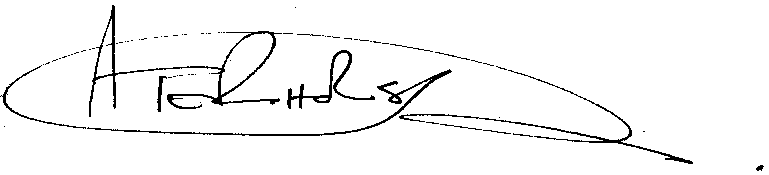
\includegraphics[width = 0.5\textwidth]{Images/Signature.png}\\
Andrew Terhorst\\
\shortdate{\today}

\addcontentsline{toc}{chapter}{Acknowledgements}
\chapter*{Acknowledgements}

This study was funded by the Commonwealth Scientific and Industrial Research Organisation (CSIRO) as part of its contribution to the Australian Research Council's Pathways to Market Industrial Transformation Hub hosted by the University of Tasmania. \medskip

\noindent
The author wishes to acknowledge the CSIRO for their extraordinary support and encouragement to get the job done. He also thanks his supervisors, Professor Dean Lusher, Associate Professor Dianne Bolton, Dr. Ian Elsum and Dr. Peng Wang. Without their input, this thesis would never have been completed. The author also wants to acknowledge fellow doctoral candidates, Bopha Roden and Sarah King, for their friendship and support. Last but not least, the author thanks the Swinburne University of Technology Higher Degree Research office for helping him navigate the rules and procedures of doctoral studies.  

\addcontentsline{toc}{chapter}{Foreword}
\chapter*{Foreword}

One must demonstrate a capacity for independent, critical thinking in a doctoral thesis. Examiners want to see evidence of originality and be presented with logical arguments. They do not want to see careless mistakes that indicate sloppy research \citep{mullins2002its}. My goal in writing this thesis was to present a rigorous and coherent analysis of tacit knowledge sharing in open innovation. It was clear early on that I would need a combination of quantitative and qualitative analysis to address all of my research questions. I learnt that reconciling different ontological and epistemological assumptions can be quite problematic in mixed-method research. This led me to embrace critical realism as my research philosophy. It allows one to consider reality in terms of observed or  measured reality, perceived or unmeasured reality, and actual reality \citep{bhaskar2013realist}. Unpacking these different realities using deductive, inductive and retroductive reasoning has been eye-opening and confidence-building. \medskip

I knew very little about social network analysis at the beginning of my doctoral studies. Because social network analysis is data-intensive, I decided to learn how to program in \texttt{R} to become more proficient at data manipulation. I completed online data science courses offered by John Hopkins University (USA), namely \enquote{Computing for Data Analysis}, \enquote{Getting and Cleaning Data}, \enquote{Exploratory Data Analysis}, and \enquote{The Data Scientist's Toolbox}. Each course took 4 weeks to complete. Having mastered basic \texttt{R} programming, I then did an 8-week online course entitled \enquote{Social Network Analysis} offered by the University of Michigan (USA). This course provided an excellent foundation in social network analysis. To cap things off, I attended a 5-day \enquote{Introduction to Social Network Analysis} course offered by Swinburne University of Technology. This course introduced me to exponential random graph models. I now consider myself a competent social network analyst. \medskip

I did not appreciate how much thought has to go into designing an online survey questionnaire until I completed an online course entitled \enquote{Questionnaire Design for Social Surveys} offered by the University of Maryland (USA). This 4-week course taught me about formulating short and unambiguous questions, avoiding responder fatigue, managing selective recall, and piloting surveys. One component of the course addressed interviewing skills. This component prompted me to explore further the theory and practice of successful interview techniques \citep[e.g.][]{kvale2008doing,seidman2012interviewing}. Coding interview transcripts was particularly challenging for me. Everybody I spoke to approached coding differently. As \citet{saldana2015coding} notes, there is no right or wrong way to go about coding. After many false starts, I managed to find a way to code that worked for me. I still have much to learn about qualitative analysis but think I managed to balance my thesis's quantitative and qualitative paradigms. Academic writing does not come easily to me. Early criticism of my writing was keenly felt. I only started to relax when it dawned upon me that I was becoming a \enquote{subject matter expert} and could communicate with authority. \medskip

There is no doubt that I learned much about open innovation through my research. I discovered the importance of tacit knowledge for problem-solving and now understand how tacit knowledge defines who we are, and what this means in terms of power and trust relations. More importantly, I recognise the importance of skilled brokerage to facilitate tacit knowledge flows in open innovation. 

\newpage
\setcounter{tocdepth}{3}
\tableofcontents

\newpage

\listoffigures

\newpage

\listoftables

\mainmatter

\chapter{Introduction}
 \section{Scope of study}

Innovation encompasses the invention, development, and implementation of new ideas \citep{garud2013perspectives}. Business enterprises are increasingly obliged to engage in continuous innovation in order to remain competitive in an ever-demanding, knowledge-based, economy \citep{lubit2001keys,urbancova2013competitive}. However, business enterprises also struggle to keep pace with technological advances and cannot rely solely upon their internal knowledge assets for innovation \citep{chesbrough2009open,enkel2009open}. Unsurprisingly, many business enterprises are turning to open innovation as a competitive strategy \citep{chesbrough2003open,enkel2009open,stanko2017under}. With open innovation, the innovation process relies heavily on accessing, absorbing, and harnessing knowledge across organisational boundaries \citep{chesbrough2017future}. \medskip

Little is known about the role of tacit knowledge in open innovation, which is remarkable, considering tacit knowledge guides the learning and thought processes that produce novel ideas \citep{leonard1998role}. Knowledge that crosses organisational boundaries is likely to have a tacit component, more so if the knowledge is very complex \citep{seidler2008use}. Despite the importance of tacit knowledge for innovation, it has received scant attention in the open innovation literature (see Figure \ref{fig:biblio}). \medskip

This thesis attempts to fill this gap by examining tacit knowledge sharing in three open innovation partnerships. Because tacit knowledge is something that is usually shared either unwittingly or voluntarily, attention focuses on how human agency and organisational structures affect tacit knowledge sharing. \medskip

\begin{figure}[p]
\centering
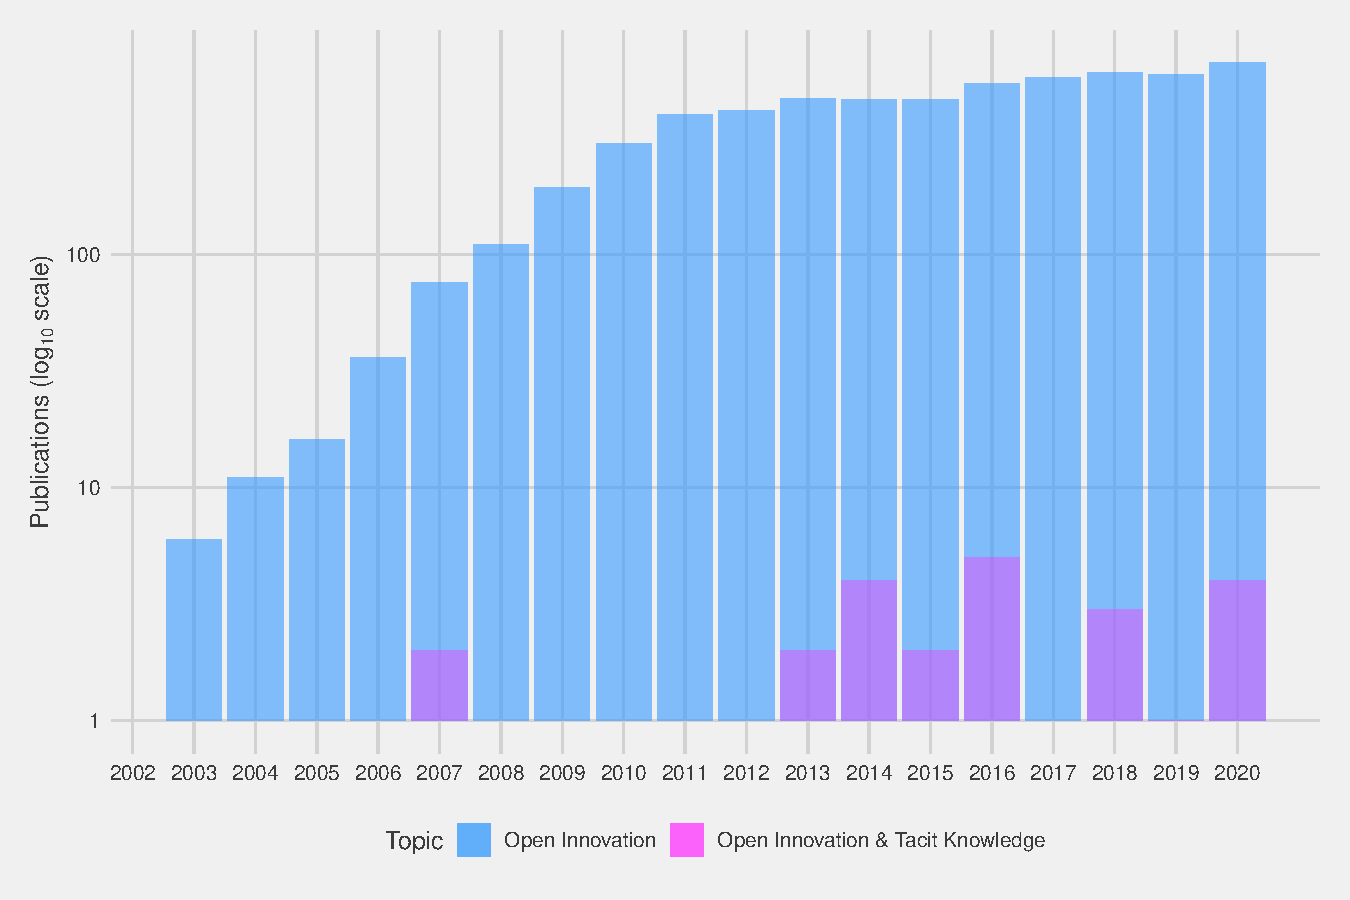
\includegraphics[width=0.9\linewidth]{Images/tk_oi.pdf}
\caption[Articles published each year on open innovation]{Articles published each year on open innovation with the relative proportion of articles referencing tacit knowledge. Few articles address tacit knowledge directly. Data from Scopus (search queries: TITLE-ABS-KEY ("open innovation") and TITLE-ABS-KEY ("tacit knowledge"  AND  "open innovation")).}
\label{fig:biblio}
\end{figure}

\section{Background}

\subsection{Trend towards open innovation} \label{sss:oi}

Proponents of the resource-based view of the firm argue that competitive advantage stems from the application of tangible and intangible resources available to it \citep{wernerfelt1984resource,peteraf1993cornerstones}. To what extent a firm can sustain competitive advantage depends on how valuable, rare, inimitable, and non-substitutable its resources are \citep{barney1991firm}. Because knowledge fuels innovation, it is arguably the most critical resource for a firm competing in a fast-moving and technology-driven economy \citep{grant1996toward,urbancova2013competitive}. However, the proliferation of increasingly sophisticated knowledge means that firms are finding it harder to compete using only their internal knowledge resources \citep{chesbrough2009open,enkel2009open}. Many firms are turning to open innovation as a competitive strategy \citep{chesbrough2003open,enkel2009open,stanko2017under}. \medskip

Open innovation is a distributed innovation process involving purposely managed knowledge flows across organisational boundaries, using mechanisms in line with the firm's business model \citep{chesbrough2014explicating}. The business model helps a firm decide what external knowledge can fuel innovation and which knowledge to release to other organisations \citep{chesbrough2017future}. Key benefits of open innovation include timely access to new knowledge or technology, sharing of risk, reduced costs of development, better customer acceptance of products or services, and enhanced ability to innovate continuously \citep{ye2013exploring}. \medskip
 
 Open innovation can be described in terms of \enquote{inbound}, \enquote{outbound} and \enquote{coupled} innovation processes \citep{gassmann2004towards}. Inbound open innovation enriches a firm's knowledge base through integrating suppliers, customers and other external actors \citep{xu2013inbound}, whereas outbound open innovation refers to the commercial exploitation of knowledge developed in-house \citep{de2016knowledge}. Coupled open innovation focuses on strategic partnerships that encompass both inbound and outbound innovation processes \citep{spithoven2013open}. Figure \ref{fig:oi_funnel} illustrates how these processes may work in practice. \medskip
 
\begin{figure}[p]
\centering
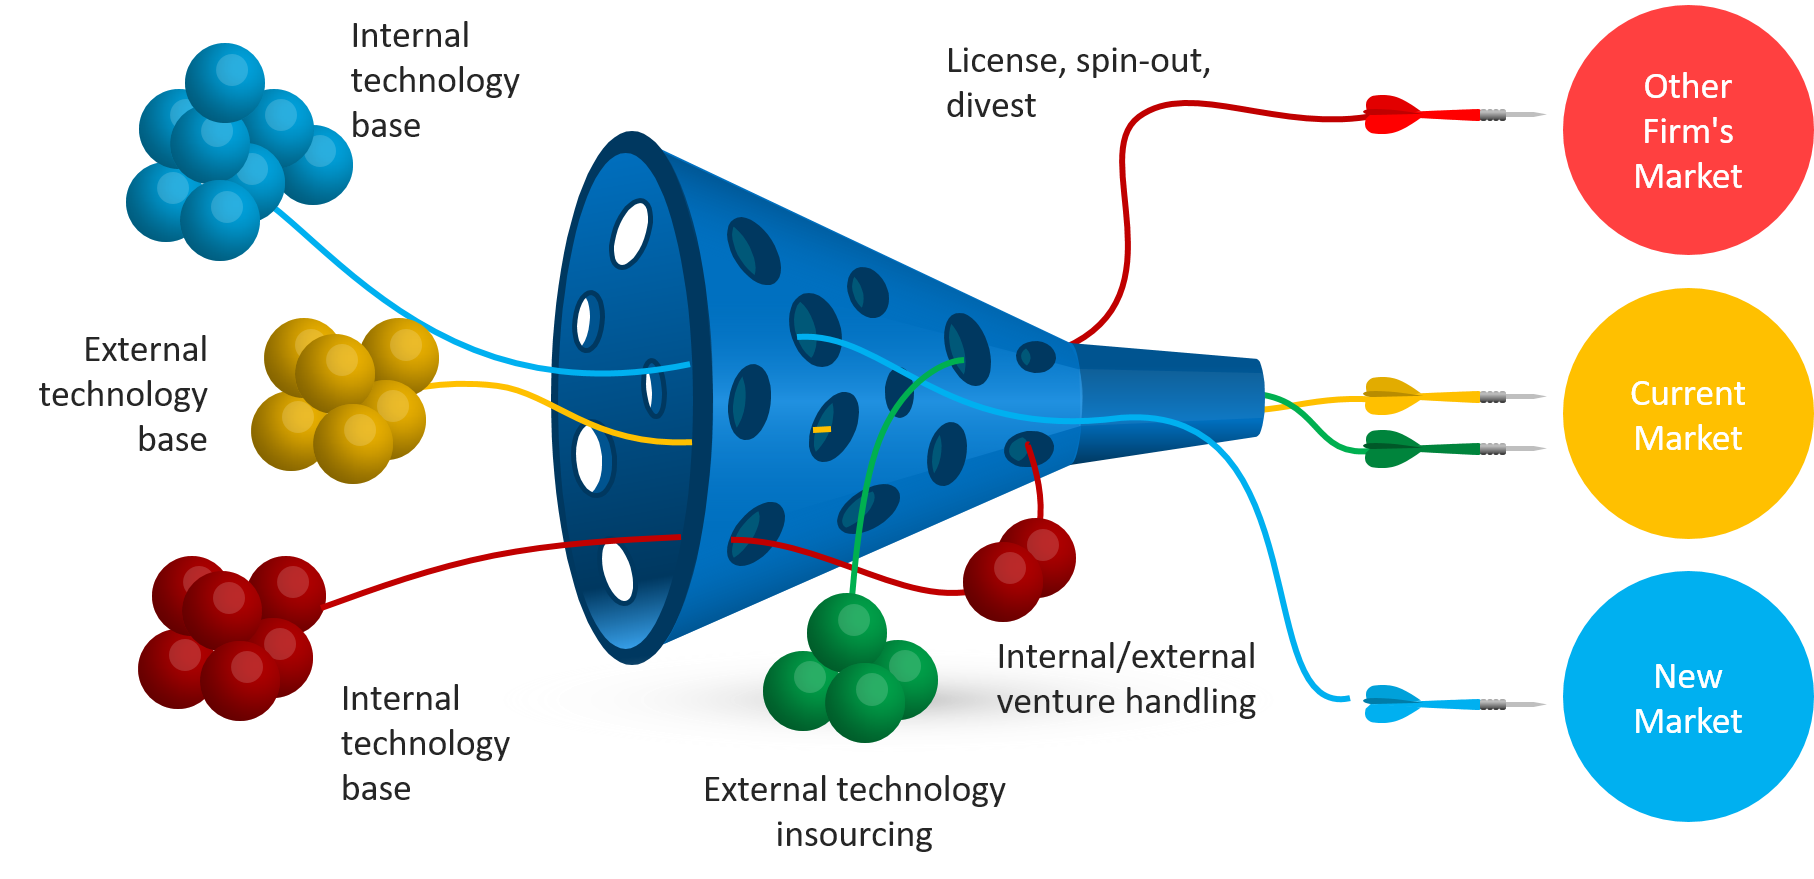
\includegraphics[width=0.9\linewidth]{Images/oi_funnel.png}
\caption[Open innovation funnel]{Open innovation funnel illustrating inbound, outbound, and coupled innovation processes. Open innovation presents multiple pathways for generating value from knowledge. How easily knowledge is able to flow across organisational boundaries depends on the strength of inter-organisational relationships and the absorptive and desorptive capacity of open innovation partner firms \citep{chesbrough2004open,lichtenthaler2010technology}.} 
\label{fig:oi_funnel}
\end{figure}

With open innovation, the locus of knowledge creation does not necessarily correspond to the locus of innovation \citep{gassmann2004towards}. In the case of inbound open innovation, the locus of innovation is inside the firm receiving new external knowledge. With outbound open innovation, the locus of innovation is external to the firm providing knowledge. The locus of innovation with coupled innovation straddles firm boundaries. Likewise, the locus of exploitation (i.e. the application of knowledge for commercial benefit) can also be different to the locus of innovation. A firm may come up with an innovative solution to a problem through inbound open innovation, but use outbound open innovation for commercial exploitation by a third-party \citep{gassmann2004towards}. A good example is Nokia Corporation. The Finnish company was a market leader in mobile telephone handsets but became sidelined when US competitors introduced more capable \textquote{smart phones} into the market. Nokia has pivoted, using its know-how in mobile telephony to provide novel cellular network solutions (e.g. fifth-generation cellular network technology (5G) and services for the Internet of Things (IoT)) to service providers (outbound open innovation). Nokia has a strategic partnership with US-based Bell Laboratories to develop next-generation communications technologies (inbound/coupled open innovation)\footnote{\url{https://www.nokia.com/system/files/2020-03/Nokia\%20Form\%2020F\%202019_0.pdf}}.  
 
\subsection{Key capabilities for open innovation}

Different capabilities are required for inbound, outbound, and coupled open innovation. Firms pursuing inbound open innovation, for instance, need absorptive capacity to make sense of, and exploit, unfamiliar external knowledge  \citep{vanhaverbeke2007connecting}. Relative differences in absorptive capacity between open innovation partners can impede knowledge integration, contribute to power imbalances, and undermine alliance performance, all of which can result in sub-optimal open innovation outcomes \citep{lane1998relative,vanhaverbeke2007connecting,zobel2016benefiting,tell2017managing}. Overcoming relative differences in absorptive capacity is crucial for successful open innovation and requires partners to have a strong learning orientation to help align thinking and reduce differences in understanding between them  \citep{nooteboom2000learning,sun2010examination,de2016knowledge}. \medskip

Firms wanting to exploit their internally developed knowledge through outbound open innovation require \enquote{desorptive capacity} to identify and act on knowledge transfer opportunities \citep{lichtenthaler2010technology}. This includes having appropriate mechanisms for managing and leveraging intellectual property \citep{chesbrough2012open,denford2018absorption}. Absorptive and desorptive capacity can be seen as two sides of the same coin, i.e. they are pull and push factors governing knowledge transfer processes \citep{dell2015absorptive}. \medskip

Another important capability needed for open innovation is the ability to develop and maintain strong and productive inter-organisational networks \citep{chesbrough2012open}. Such an ability requires people who can operate effectively across organisational boundaries \citep{tushman1981boundary,levin2004strength,meyer2010rise}. Effective boundary spanners are not only able to broker new relations that extend or widen existing inter-organisational knowledge networks, but also play a key role in building trust and reducing the cognitive distance between open innovation partners \citep{fleming2007brokerage,goffin2010managing,renzl2008trust,sankowska2013relationships,kucharska2016trust}. 

\subsection{Role of tacit knowledge in open innovation}

\citet{kreutz2014catalyzing} define tacit knowledge as the \enquote{unwritten, unspoken, and hidden vast storehouse of knowledge held by practically every normal human being, based on his or her emotions, experiences, insights, intuition, observations, and internalised information}. They go on to state that \enquote{like the submerged part of an iceberg, tacit knowledge constitutes the bulk of what one knows, and forms the underlying framework that makes explicit knowledge possible}. Tacit knowledge provides important context for making sense of explicit knowledge, especially if such knowledge is highly specialised or complex \citep{von1994sticky,szulanski1996exploring,leonard1998role,seidler2008use}. \medskip

The leading edge of the firm’s learning often is found in the tacit knowledge of its employees \citep{horvath2000working}. Indeed, tacit knowledge is strongly implicated in innovation as it guides the learning and thought processes that produce novel ideas \citep{leonard1998role,amar2008descriptive,leonard2014knowledge}. Tacit knowledge helps bridge cognitive gaps and thus underpins a firm's absorptive capacity. Because tacit knowledge is embodied in people and embedded in the things they create, it helps a firm resist imitation by competitors \citep{horvath2000working}. \medskip

Not only is tacit knowledge deeply rooted in personal experience, it is also inculcated in group practice and culture, usually in the form of unwritten rules and procedures \citep{nonaka1995knowledge,howells1996tacit}. Some argue that tacit knowledge is a defining feature of the various sub-cultures that exist within a firm \citep[e.g.][]{smith2001role,munoz2015tacit}. Mobilising tacit knowledge in open innovation is challenging because individuals or groups are either unaware of the tacit dimension of their knowledge, or are unable to express what they know \citep{polanyi1966tacit}. Many firms do not appreciate the depth of their knowledge base and lack processes to unlock the potential value of tacit knowledge embodied in the minds and actions of employees \citep{nonaka1994dynamic,howells1996tacit,horvath2000working}. \medskip

Moreover, people cannot be coerced to share their tacit knowledge. Agency lies at the heart of tacit knowledge sharing \citep{polanyi1966tacit, emirbayer1994network}. However, finding the right balance between structure and agency is a challenge \citep{davis2010agency}. Too much structure may inhibit participants' willingness to share tacit knowledge or contribute ideas. Conversely, too little structure can make goals less clear, leading to unsatisfactory open innovation outcomes \citep{lam2000tacit}. \medskip

Adding to the challenge is the notion that tacit knowledge is not transferred but rather interpreted within a specific context \citep{nonaka1995knowledge,duguid2005art,marabelli2014knowing,zhang2020extended}. Face-to-face social interaction is key because it allows immediate feedback to confirm understanding and correct any misinterpretations \citep{haldin2000difficulties,gertler2003tacit,koskinen2003tacit}. While advances in information technology (e.g. e-mail, instant messaging, video-conferencing, web-based collaboration platforms, and augmented or virtual reality) make it easier for dispersed team members to communicate with each other, much of this information technology is not that well-suited for tacit knowledge exchange. Limited face-to-face interaction may negatively impact knowledge sharing and idea generation in open innovation \citep{johannessen2001mismanagement}. Neglecting the tacit dimension of inter-organisational knowledge exchanges may result in sub-optimal, or even worse, failed open innovation outcomes. 

\section{Research opportunity}

\subsection{A network perspective of open innovation}

Since open innovation involves multiple organisations exchanging knowledge with one another, this study conceptualises an open innovation partnership as a temporary knowledge network, one that is deliberately set up to achieve a specific innovation outcome within a market-relevant time frame \citep{perez2013temporary,cococcioni2014exploring,terhorst2018tacit}. Knowledge networks represent collections of individuals and teams that come together across organisational, spatial and disciplinary boundaries to create, share or apply a body of knowledge \citep{pugh2013designing}. Though tacit knowledge has a key role to play in transferring specialised or complex knowledge \citep{davenport1998working,sternberg1999tacit,johnson2002all,endres2007tacit,tell2017managing}, the extent to which it helps bridge cognitive gaps and stimulate idea generation is poorly understood. As tacit knowledge exchange is a socially intensive process, there is merit in using social network analysis to assess tacit knowledge flows in open innovation \citep{leonard1998role,busch2000graphically,zhu2007social}. Such analysis can provide useful insights into both endogenous (inherent) and exogenous (environmental) factors that influence tacit knowledge transfer processes \citep{kolleck2013social,tortoriello2015social}. 

\subsection{Exploring motivational factors}

Tacit knowledge requires significantly more effort to communicate than explicit knowledge. It requires commitment to learn from, or to teach, others. In other words, individuals have to be sufficiently motivated to seek out and share tacit knowledge \citep{leonard1998role}. Motivation is a theoretical construct used to explain individual behaviour. More specifically, a motive is what prompts a person to act in a specific way or develop an inclination towards a particular behaviour \citep{pardee1990motivation}. Past studies show a significant and positive relation between an individual's level of intrinsic motivation and the amount of tacit knowledge they share \citep[e.g.][]{osterloh2000motivation,kaser2001knowledge,smith2001role}. Intrinsic motivation is about engaging in activities because these are enjoyable or personally meaningful \citep{ryan2000intrinsic}. Although these studies highlight the importance of personal motivation, the psychosocial processes underpinning tacit knowledge exchange in open innovation are not well understood. Open innovation is unlikely to succeed without highly motivated agents.

\subsection{Unpacking power-relations} 

Though it is often stated that \enquote{knowledge is power}, not much is written about power and power-relations in the knowledge management literature \citep{haugaard2012rethinking}. The current literature on power is dominated by two contrasting views of power, namely \textquote{power as domination}, also referred to as \textquote{power-over}, and \textquote{power as empowerment}, often characterised as \textquote{power-to} \citep{haugaard2012rethinking}.  People accumulate tacit knowledge to empower themselves in their quest for competence or self-efficacy \citep{endres2007tacit}. By sharing their tacit knowledge, individuals are essentially empowering others to perform work more independently and confidently \citep{bordum2002tacit,lin2007share}. Some people may be reluctant to share their hard-earned tacit knowledge if they think this will compromise or dis-empower them. \medskip

The network perspective treats power as inherently relational \citep{ibarra1993power}. As mentioned earlier, knowledge brokers play a vital role in open innovation as they connect individuals, coordinate interactions between partners, and help others make sense of unfamiliar knowledge. By virtue of their network position, they are able to exert considerable influence over knowledge flows. By examining patterns of brokerage in knowledge networks, one may be able to infer how partners exercise power in open innovation. The patterns should reveal who is being empowered through knowledge exchanges and highlight which brokerage mechanisms are the most significant in an open innovation partnership. 

\section{Thesis objectives}

This thesis employs mixed-method social network analysis to explore tacit knowledge sharing in three open innovation partnerships. Mixed-method social network analysis enables the exploration of network structure while not forsaking the qualitative observations about what is going on within a network, e.g. external social forces, mechanisms and structures that shape tacit knowledge sharing relations \citep{crossley2010social}. Using a mixed methods is fraught because of the complex ontological and epistemological issues involved \citep{giddings2006mixed,mcevoy2006critical}. Consequently, this thesis embraces a critical realist worldview to make sense of data collected under different epistemological assumptions \citep{johnson2004mixed,giddings2006mixed,welch2011theorising}. \medskip

As tacit knowledge sharing is primarily an act of volition or free-will, the thesis considers how agency and structure affect tacit knowledge sharing in open innovation. The network analysis investigates the extent to which self-determination influences tacit knowledge sharing, whether tacit knowledge sharing is more or less likely to happen in the presence of other ties, and what patterns of brokerage reveal about partner behaviour in open innovation networks. This analysis is complemented by semi-structured interviews that capture the industrial, organisational, and cultural contexts governing the emergence of collaborative social structures that support tacit knowledge sharing. Four research questions are addressed in this study: \medskip

\begin{enumerate}
\item What does the structure of tacit knowledge networks reveal about knowledge enacted in practice?
\item Does brokerage differ according to the type of knowledge being exchanged?
\item To what extent does self-determination drive tacit knowledge sharing in open innovation?
\item What does the micro-structure of tacit knowledge networks reveal about trust and power-relations in open innovation partnerships?
\end{enumerate}

\section{Research contribution}

This thesis advances knowledge by providing fresh insight into how tacit knowledge sharing facilitates learning in open innovation partnerships. It also breaks new ground by examining how brokerage roles vary according to the amount of tacit knowledge being exchanged and what this means in terms of power-relations. By embracing a social network perspective, this thesis draws attention to key social processes affecting tacit knowledge sharing in open innovation. This should help managers devise more effective strategies for transferring complex or specialised (also referred to as \textquote{sticky}) knowledge across organisational boundaries. Another contribution of this thesis will be the development and testing of a more robust framework for mixed-method social network analysis that others can use. 

\section{Document structure}

The remainder of this document is organised as follows:

\begin{itemize}[leftmargin=0pt]
    \item[] \textbf{Chapter 2} considers the epistemology of knowledge and what this means in terms of absorptive capacity and knowledge brokerage.
    \item[] \textbf{Chapter 3} reviews key literature on motivation, trust, and power relevant to tacit knowledge sharing. \textbf{Chapters 2 and 3} present a number of propositions that inform the subsequent mixed-method analysis. The propositions address key aspects of the four research questions. 
    
    \item[] \textbf{Chapter 4} describes the critical realist research methodology underpinning this study. This includes a justification for using mixed-methods and details the quantitative and qualitative procedures used to collect and analyse data.
    \item[] \textbf{Chapter 5} describes and contrasts the three open innovation partnerships investigated in this study.
    \item[] \textbf{Chapter 6} presents the results of the statistical network analysis that examined the role of motivation, trust, and power in tacit and explicit knowledge exchanges, and the significance of different broker roles in each case.
    \item[] \textbf{Chapter 7} presents the results of the qualitative analysis of the semi-structured interviews.
    \item[] \textbf{Chapter 8} discusses the quantitative and qualitative results from a critical realist perspective. 
    \item[] \textbf{Chapter 9} summarises the main findings of this study and reflects on some key lessons learned as this study unfolded. This includes descriptions of the study's limitations and possible avenues for future research. 
\end{itemize}

\chapter{Knowledge networks}

\section{Introduction}

The previous chapter conceptualised an open innovation partnership as a temporary knowledge network deliberately set up to achieve a specific innovation outcome within a market-relevant time frame. The previous chapter also highlighted the importance of tacit knowledge for open innovation. Tacit knowledge exchange is a socially intensive process and embracing a network perspective offers valuable insights into the endogenous and exogenous factors influencing tacit knowledge transfer processes. \medskip

This chapter considers the nature of knowledge and how this affects absorptive capacity and knowledge brokerage in open innovation. As a reminder, absorptive capacity is the ability of a firm to value, acquire, assimilate, transform, and exploit new external knowledge \citep{cohen1990absorptive}. Knowledge brokerage is about connecting people with knowledge to those who need it. Although there are many aspects to managing knowledge flows across organisational boundaries, this chapter makes the case that open innovation is mainly about facilitating the interaction between know-how (practical knowledge on how to accomplish something) and know-what (factual knowledge) \citep{winter1987knowledge,garud1997distinction}. Other forms of knowledge are know-who (knowing who has relevant know-how), know-why (scientific understanding), and know-when (knowing when to apply know-how) \citep{hulme2014editorial}. \medskip

Theoretical concepts are used to formulate propositions about tacit knowledge sharing in open innovation. This study is exploratory, and the propositions are less about testing specific hypotheses about tacit knowledge sharing as they are about gaining a more in-depth understanding of the social mechanisms that underpin tacit knowledge sharing. 

\section{The nature of knowledge}

Traditionally knowledge is considered a justified true belief \citep{bolisani2018elusive}. For those who embrace a positivist worldview, truthfulness is the main feature of knowledge. They see knowledge as objective, static, and absolute. Others who embrace a constructivist or pragmatic worldview, place more weight on justified beliefs. For them, the utility of knowledge is more important than truthfulness \citep{bolisani2018elusive}. \citet{spender1996organizational} observes that \enquote{knowledge is less about truth and reason and more about the practice of intervening knowledgeably and purposefully in the world}. What matters is not what we know, but knowing how to apply our knowledge \citep{ryle1949concept,orlikowski2002knowing}. \medskip

It is useful to think about how people know things. Two perspectives dominate the theory of knowledge: rationalism and empiricism. Rationalism argues that knowledge is the result of a reasoning process. Knowledge exists in our minds. What is observed or sensed does not constitute knowledge \citep{russell2009human}. Empiricism, on the other hand, argues that knowledge is a product of our sensory interface with the real world \citep{bolisani2018elusive}. \medskip

The distinction between rationalism and empiricism becomes useful when interpreted to mean that humans know in two ways, either through experience or via reasoning. When these two ways of knowing interact, new knowledge is created \citep{spender1996making,bolisani2018elusive}. \citet{cook1999bridging} consider knowledge in terms of the epistemology of possession and the epistemology of practice. The epistemology of possession treats knowledge as something people possess (know-what or know-that), whereas the epistemology of practice refers to knowing how to enact knowledge in practice (know-how). Know-how is the ability to put know-what into practice \citep{cook1999bridging,tsoukas2001organizational}. \medskip

\citet{polanyi1966tacit} states that people often know how to do things by adhering to a set of rules they are unaware of. He refers to this unknown set of rules for skilful action as tacit knowledge (or tacit knowing, to be more precise). People accumulate tacit knowledge through observation, imitation, and repeated interaction. Tacit knowledge is deeply rooted in personal experience \citep{nonaka1995knowledge}. Not only is tacit knowledge embodied in the minds and actions of individuals, but it also manifest in group practice and culture, usually in the form of unwritten rules and procedures \citep{munoz2015tacit}. \medskip

The innovation process is all about transforming ideas into reality \citep{garud2013perspectives}. It involves applying know-how to new or existing knowledge in novel ways \citep{van1986central,quintane2011innovation}. In that case, open innovation is less about managing knowledge flows as it is about bringing know-how and know-what together. Sharing know-how enables others to learn the practice that entails the know-how. Thus, open innovation entails helping others develop the ability to apply knowing and knowledge in new and different contexts \citep{van1986central}. 

\section{Knowledge networks}

A knowledge network connects individual and organisational actors across organisational, spatial, and disciplinary boundaries to create, share, or apply a body of knowledge \citep{pugh2013designing}. Some researchers distinguish between a knowledge network and a social network \citep[e.g.][]{yayavaram2008decomposability,wang2014knowledge,brennecke2017firm}. Such a distinction is warranted if one treats people and knowledge as separable entities. As tacit knowledge is embodied in the minds and actions of people, such a distinction not appropriate for this thesis. Instead, this thesis treats a knowledge network as a social network, where ties represent social interactions between knowledgeable actors. \medskip

The value a firm can extract from its knowledge network depends on the reach of firm's ties to diverse and distant partners, the richness of knowledge embedded in the network, and how easily a firm can harness its network resources \citep{gulati2011networks}. We can describe a firm's reach in terms of its weak knowledge ties \citep{hansen1999search}. Actors connected by strong ties often share similar interests and are privy to the same knowledge. Strong ties tend to make people look inward and be less receptive to external knowledge. Actors connected by weak ties tend to mix in different social circles and are thus more exposed to different knowledge and opportunities \citep{granovetter1973strength}. \medskip

Regarding the richness of knowledge resources, the depth of knowledge and quality of knowledge is of primary importance, as this determines the potential value of the knowledge resource \citep{davenport1998working,kane2005knowledge}. The depth of knowledge reflects its usefulness for problem-solving. Addressing simple problems requires basic know-how. As problems become increasing complex, higher levels of cognition are required. Deeper know-how is required to solve more challenging problems \citep{webb2002depth,bennet2008depth}. The quality of knowledge can be described in terms of its usability, completeness, currency, and accuracy \citep{wixom2005theoretical}. \medskip

How easily open innovation partners can harness knowledge embedded in a network depends on a number of factors. Knowledge that is complex usually has a significant tacit component to it. Transferring complex knowledge is difficult because it involves transferring know-how between partners as well. The human dimension of such knowledge makes it particularly \enquote{sticky} \citep{von1994sticky,szulanski2003sticky}. \medskip

Different levels of openness can lead to a breakdown of trust and loss of enthusiasm between open innovation partners \citep{laursen2014paradox,dragsdahl2019perspective}. How open a firm is in an open innovation partnership is usually determined by its appropriability regime. An appropriability regime refers to the mechanisms put in place by a firm to prevent knowledge being appropriated by imitators \citep{teece1998capturing,hurmelinna2008appropriability}. It is not always clear to other firms in the partnership how this works. One way to resolve this is by making appropriability regimes more explicit from the outset \citep{gama2019managing}. \medskip

Relative differences in absorptive capacity between open innovation partners can also impede efforts to combine or integrate different ways of knowing \citep{vanhaverbeke2007connecting,lichtenthaler2016absorptive}. Spatial proximity is another factor. Achieving interaction between different ways of knowing is difficult when partners are not in close proximity to each other \citep{wineman2009spatial,roper2018knowledge}. \medskip

Focusing on the structure of knowledge networks, a structural hole refers to gaps between disconnected groups of people \citep{burt2000network}. Groups on either side of the structural hole are privy to different knowledge. Members of tightly-knit groups are more likely to work with tacit knowledge in the form of mutually understood, unwritten language and routines to coordinate with one another \citep{burt2007secondhand}. Structural holes present an opportunity to broker knowledge exchanges between otherwise disconnected groups of people. A knowledge network with an abundance of structural holes facilitates innovation by allowing strategically placed actors to access and combine diverse knowledge in novel ways \citep{burt2004structural,sparrowe2011publishing}. \medskip

Because tacit knowledge familiar within groups is likely to be invisible to other groups, it can yield a premium to brokers who can coordinate such knowledge across the groups \citep{burt2007secondhand}. While brokerage across structural holes in a disconnected knowledge network is the source of value, network closure is critical to realising the value buried in structural holes \citep{burt2004structural,rost2011strength}. Network closure refers to a human tendency to form into social groups. More closed networks with fewer structural holes promote trust and reduce opportunism leading to more productive collaboration from the perspective of knowledge sharing \citep{ahuja2000collaboration}. \medskip

In summary, we conceive an open innovation partnership as a temporary knowledge network set up to achieve a specific innovation outcome. Extracting value from a knowledge network depends on network reach, the depth and quality of relevant knowledge embedded in the network, and the ability of partners to leverage knowledge resources. While connections across structural holes is a source of value in a knowledge network, network closure is vital for realising the value buried in structural holes. Hence, \bigskip

\begin{tcolorbox}
\textit{\textbf{Proposition 1a:} Open  innovation  requires  practitioners  to  connect across organisational and disciplinary boundaries so that they can apply their know-how in novel ways. (Research Question 1).}
\end{tcolorbox}

\section{Absorptive capacity} 

Thus far, we have examined how value may be extracted from temporary knowledge networks by bridging structural holes and achieving network closure. Without network closure, interaction between open innovation partners who possess the knowledge and other partners who know how to apply it, is well nigh impossible. However, the ability to generate value through such interaction is contingent on the absorptive capacity of the latter \citep{vanhaverbeke2007connecting,lichtenthaler2009capability,robertson2012managing,xia2016unpacking}. \medskip

Absorptive capacity is the \enquote{ability of a firm to recognise the value of new, external information, assimilate it, and apply it to commercial ends} \citep{cohen1990absorptive}. Despite being the subject of countless studies, the extent to which absorptive capacity contributes to firm performance is still an open issue \citep{omidvar2013revisiting,duchek2013capturing}. Open innovation puts the organisational practices used to source external knowledge into sharp focus. Treating an open innovation partnership as a temporary knowledge network opens new avenues to explore practices that build absorptive capacity \citep{vanhaverbeke2007connecting,xia2016unpacking}. \medskip

What is absorptive capacity exactly? \citet{cohen1990absorptive} embrace a cognitive approach to absorptive capacity by connecting ideas from individual learning to organisations. According to them, the amount of experiential knowledge a firm can accumulate through its employees determines its absorptive capacity. They view the relationship between absorptive capacity and the level of experiential knowledge as a positive feedback loop, where an increase in absorptive capacity improves the level of relevant knowledge, which in turn further increases absorptive capacity. Mediating this feedback loop is the environment the firm operates in \citep{van1999coevolution}. \citet{lane1998relative} suggest that absorptive capacity is more about the ability of a firm to learn from another. This ability is a function of not only the extent to which firms have overlapping knowledge bases but also the extent to which they socially interact \citep{dyer1998relational,nooteboom2000learning}. \medskip

Early studies paid little attention to the processes that build absorptive capacity leading \citet{zahra2002absorptive} to re-conceptualise absorptive capacity as a dynamic capability that integrates internal processes for acquiring, assimilating, transforming, and exploiting external knowledge. They describe knowledge acquisition as the ability of a firm to identify and acquire externally generated knowledge critical to its operation. Knowledge assimilation encompasses the processes used by a firm to make sense of externally sourced knowledge, whereas knowledge transformation refers to the processes used by a firm to integrate assimilated external knowledge with existing internal knowledge. Knowledge exploitation is about the processes used by a firm to enhance existing competencies or create new ones by incorporating acquired and transformed knowledge into its operations. \citet{zahra2002absorptive} distinguish between potential absorptive capacity, namely the capability to acquire and assimilate new external knowledge, and realised absorptive capacity, which is the capability to transform and exploit knowledge. They suggest the ratio of realised absorptive capacity to potential absorptive capacity measures the efficiency of an organisation at leveraging absorbed knowledge. \citet{zahra2002absorptive} also highlight the importance of social mechanisms that connect people who acquire external knowledge with people inside the firm who can apply this knowledge. \citet{jansen2005managing} find coordination capabilities, specifically brokerage, shared decision-making and job rotation, enhance potential absorptive capacity, whereas socialisation capabilities increase realised absorptive capacity. \medskip

\citet{todorova2007absorptive} highlight how different appropriability mechanisms and power relations may influence absorptive capacity.  Firms may employ several mechanisms to protect their knowledge from being appropriated by others. How and when these are applied is often unclear and can create tension between knowledge sharing and knowledge protection practices \citep{gama2019managing}. Firms do not want to leak valuable knowledge as quickly as they absorb it \citep{todorova2007absorptive}. The tension between knowledge sharing and knowledge protection can thwart inter-organisational learning that is needed to overcome relative differences in absorptive capacity \citep{dragsdahl2019perspective,gama2019managing}. Regarding power relations, \citet{todorova2007absorptive} claim power relations inside the firm moderate the assimilation and transformation of knowledge, while power relations between partners moderate the relationship between absorptive capacity and competitive advantage.  \citet{easterby2008absorptive} observe that political acts by brokers affect access to external knowledge, while diffusion of knowledge within a firm depends on the extent to which employees are empowered. \citet{easterby2008absorptive} also highlight the importance of boundaries and how these affect absorptive capacity processes. The permeability of boundaries determines the ease of transferring knowledge. They consider power and boundaries as central features of a process view of absorptive capacity. \medskip

\citet{marabelli2014knowing} interpret a firm's absorptive capacity in terms of the epistemology of possession and the epistemology of practice. They differentiate between knowledge that resides in the minds of people, which can be spread by individuals able to develop a shared understanding with others, and sticky knowledge enacted in practice. The epistemology of practice treats absorptive capacity as a capability that emerges when applying knowledge in practice. \citet{marabelli2014knowing} argue that a practice-based perspective provides a more nuanced perspective of power and how it shapes absorptive capacity. They refer to prohibitive and productive power (also referred to as power-over and power-to, respectively). Prohibitive power focuses on the power of organisational actors to control knowledge and achieve objectives at the expense of others. Productive power, on the other hand, focuses on empowering (or dis-empowering) actors to change knowledge practices. \medskip

\citet {lichtenthaler2016absorptive} argues past studies have overlooked the negative consequences of building absorptive capacity. These include challenges around capturing value from knowledge, overemphasis on prior-related knowledge, and inter-dependencies between internal processes. The challenges around capturing value relate to the capabilities needed to manage increasingly sophisticated knowledge and the rising cost of capability development. \citet{lichtenthaler2016absorptive} claims that firms struggle to capture value from tacit knowledge and prior-related knowledge may be of limited use when it comes to adapting and transforming knowledge for use in new contexts. Firms may not benefit from externally sourced knowledge because it may decay over time. \medskip

Firms pursue open innovation because they cannot develop the know-how or expertise needed to remain competitive fast enough. They require absorptive capacity to capture value from their knowledge networks but building absorptive capacity requires significant social interaction to support learning and the application of knowledge in practice. How partners manage their appropriability regimes may stand in the way of this. Absorptive capacity is also affected by the way power is exercised at both the individual and organisational level. \bigskip

\begin{tcolorbox}
\textit{\textbf{Proposition 1b:} Reducing cognitive distance between open innovation partners  requires  significant  social  interaction  to support learning and the application of knowledge in practice (Research Question 1).}
\end{tcolorbox}

\section{Knowledge brokerage}

Brokerage may be defined as the \enquote{behaviour by which an actor influences, manages, or facilitates interactions between other actors} \citep{obstfeld2014brokerage}. Knowledge brokers make connections between those who need knowledge and those who have it i.e. they apply their know-who to connect people with the relevant know-how \citep{davenport1998working}. From a network perspective, brokers bridge structural holes and are able to use their position to influence access to knowledge resources through their network of weak ties \citep{burt1992structural,hanneman2005introduction,davis2010agency,simpson2011network,stovel2012brokerage}. From a practice perspective, brokers facilitate the integration and synthesis of knowledge provided by others. Both approaches invoke the use of power, but a critical distinction between them is that brokers in open innovation partnerships are less likely to operate only out of self-interest \citep{lingo2010nexus,marabelli2016strategic}. \medskip

\citet{obstfeld2014brokerage} describe three strategic orientations to brokerage: \enquote{conduit}, \enquote{tertius gaudens}, and \enquote{tertius inungens} brokerage. Conduit brokerage is about a third-party who transfers information, knowledge, or resources between two disconnected parties. The broker mediates rather than moderates the relationship between two others and may help them synthesise new knowledge. Tertius gaudens refers to \enquote{the third who enjoys} \citep{simmel1950sociology}. With tertius gaudens brokerage, the broker aims to exploit differences between two parties by either keeping them apart or playing one against another. In contrast, tertius iungens (\enquote{the third who joins}) brokerage is about a third-party who introduces two otherwise disconnected parties to each other and encourages them to collaborate (Table \ref{tab:brokerage}). \medskip


\begin{sidewaystable}
\resizebox{0.9\textwidth}{!}{
\begin{threeparttable}
\footnotesize
\setlength{\tabcolsep}{6pt}
\renewcommand{\arraystretch}{1}
\caption{Brokerage processes \citep{obstfeld2014brokerage}.}
\label{tab:brokerage}
\begin{tabular*}{\textwidth}{>{\raggedright}p{5cm}>{\raggedright\arraybackslash}p{6cm}>{\raggedright\arraybackslash}p{6cm}>{\raggedright\arraybackslash}p{6cm}}
\toprule
& \multicolumn{1}{c}{Conduit} & \multicolumn{1}{c}{Tertius Gaudens} & \multicolumn{1}{c}{Tertius Iungens} \\ 
\midrule
& \begin{minipage}{0.2\textwidth} \centering 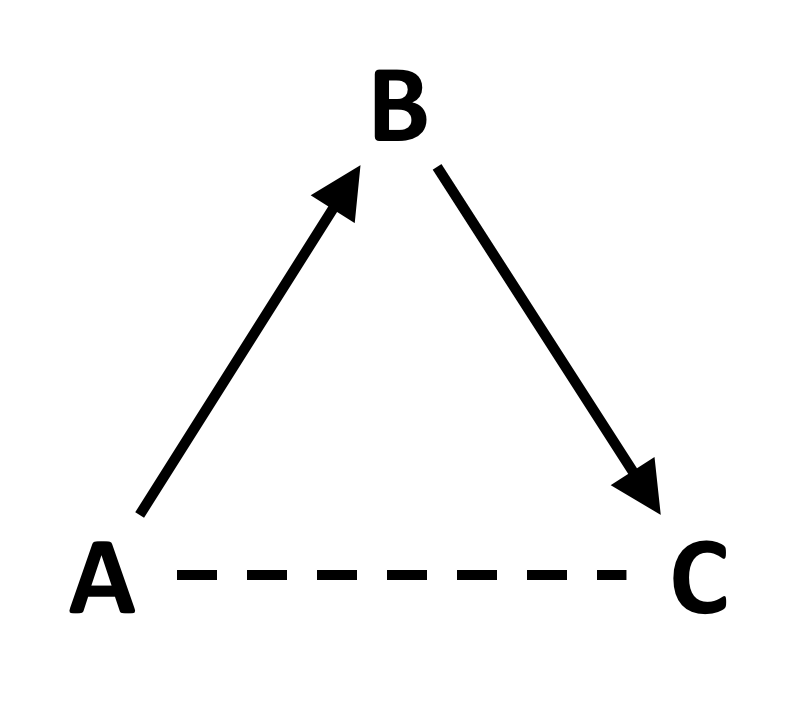
\includegraphics[width=0.7\linewidth]{Images/CDT_brokerage} \end{minipage}  & \begin{minipage}{0.2\textwidth} \centering 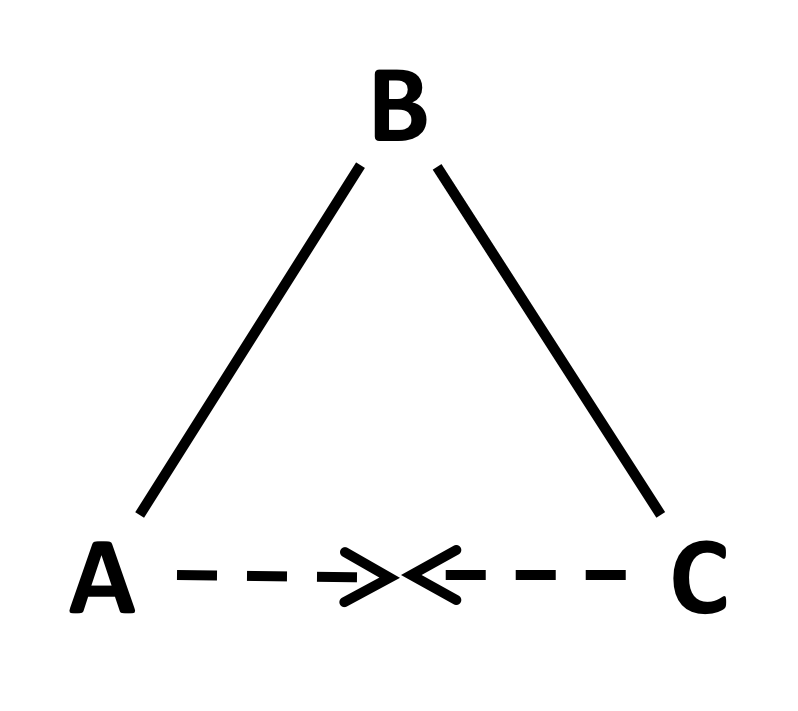
\includegraphics[width=0.7\linewidth]{Images/TG_brokerage_1} \end{minipage}  & \begin{minipage}{0.2\textwidth} \centering 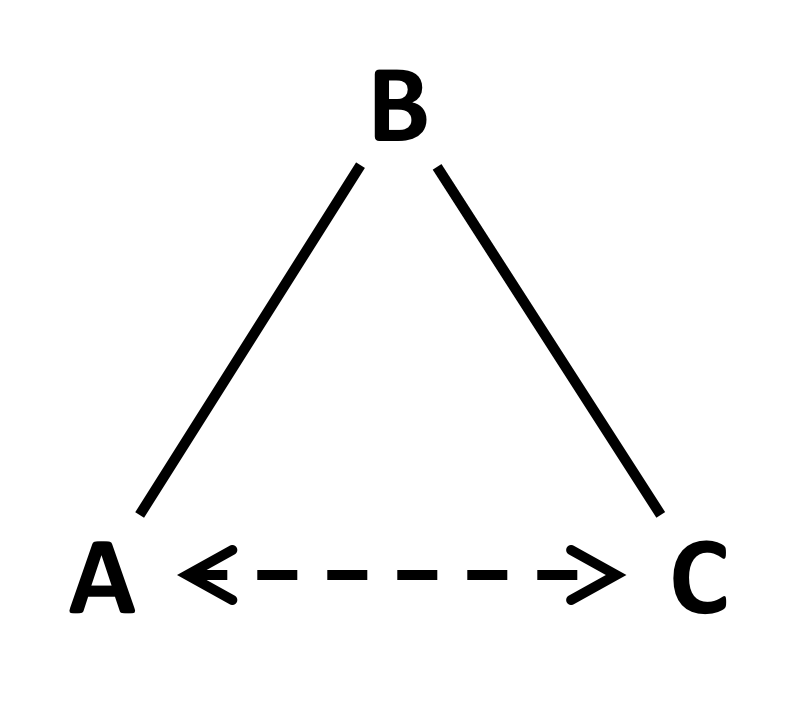
\includegraphics[width=0.7\linewidth]{Images/TI_brokerage} \end{minipage}   \\
&  & \begin{minipage}{0.2\textwidth} \centering 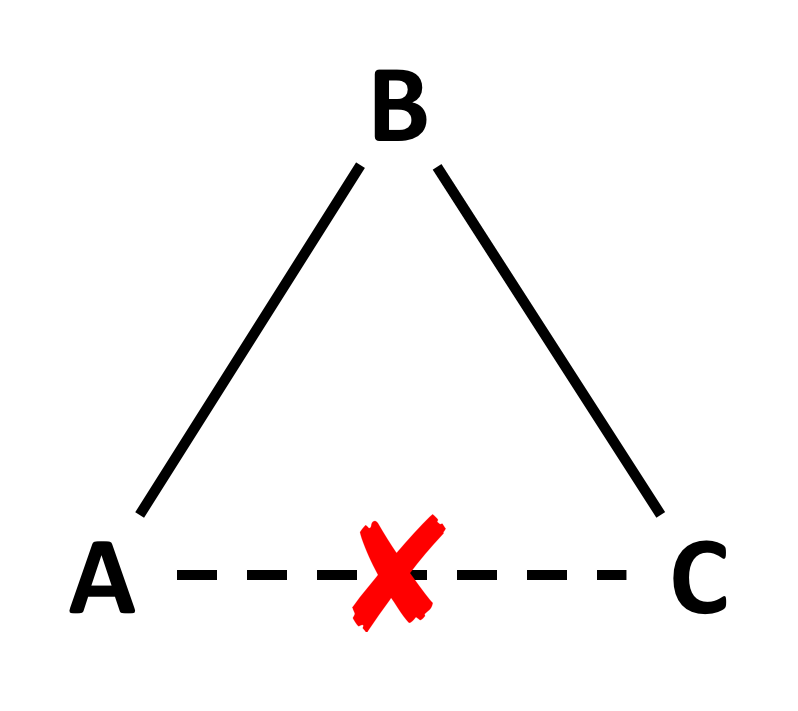
\includegraphics[width=0.7\linewidth]{Images/TG_brokerage_2} \end{minipage}  & \\
\midrule
Open network\\(absence of A-C tie) & B transfers information, knowledge, or other resources between A and C, where A and C have no prospect of meeting. & B plays A and C against one another or keeps A and C apart. & B introduces A and C where A and C have no prior tie. \\
\midrule
Closed Network\\(presence of A-C tie) & B facilitates transfer between A and C and may help synthesise new knowledge. & B cultivates conflict, competition, or separation between A and C (divide et impera) & B coordinates new collaborative action between A and C.  \\ 
\bottomrule
\end{tabular*}
\end{threeparttable}
}
\end{sidewaystable}


Each orientation expresses a different power dynamic. Whereas tertius gaudens brokerage is about exercising power over others, conduit and tertius iungens brokerage are mostly about empowering others \citep{fleming2007collaborative,obstfeld2014brokerage}. Skilled brokerage often involves the selective deployment of these approaches with different actors or for different objectives. Different combinations of tertius iungens and tertius gaudens behaviour are necessary to tailor brokerage strategies to match the situation \citep{lingo2010nexus,obstfeld2014brokerage,quintane2016brokers}. \medskip

Brokerage is also transient. The ability to engage in tertius gaudens brokerage diminishes when other actors engage in balancing operations to avoid or side-step power-dependencies \citep{emerson1962power}. Likewise, once a broker has introduced one actor to another through conduit or tertius iungens brokerage, their job of empowering others is complete \citep{obstfeld2014brokerage}. Brokers who have outlived their usefulness in a particular situation often go on to seek out new brokerage opportunities. In that way, brokers drive the expansion and evolution of existing networks \citep{obstfeld2014brokerage,quintane2016brokers}. \medskip

From an open innovation perspective, tertius iungens brokerage is essential, especially in the early stages of collaboration, when many actors do not know fellow collaborators in partner organisations very well \citep{fleming2007collaborative}. Knowledge held by third parties is also likely to be unfamiliar, and brokers help others make sense of it. Once ties have formed through tertius iungens brokerage, conduit brokerage is needed to sustain trust and help synthesise and transform knowledge into novel ideas \citep{quintane2016brokers}. \medskip 

When actors belong to distinct groups, group membership may be used to categorise brokerage into five social roles. Brokers can operate as internal coordinators, in a liaison role, as a representative, as a gatekeeper, or as a mediator (also referred to as an itinerant broker) depending on their network position \citep{gould1989structures}. Figure \ref{fig:gf_roles} depicts the network configuration of each role. The breakdown of broker roles should provide interesting insights into the character of the open innovation partnership \citep{spiro2013extended}. For example, a partner heavily invested in gatekeeping is likely to be more interested in empowering themselves at the expense of others in the partnership. Alternatively, partners who operate mostly in a representative or liaison broker role are likely to be more invested in the partnership and keen to empower others \citep{spiro2013extended}. \medskip

\begin{figure}
\centering
  \begin{subfigure}[b]{0.25\textwidth}
    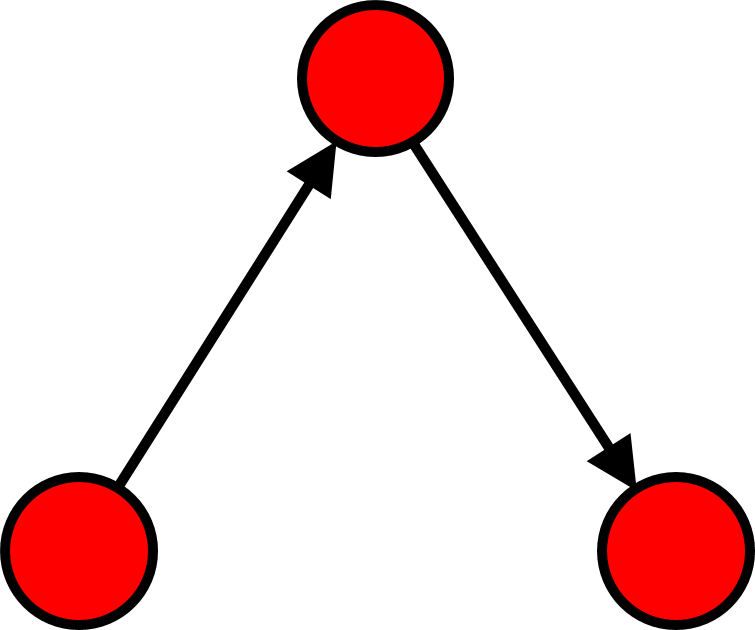
\includegraphics[width=\textwidth]{Images/w_I.png}
    \caption{Coordinator}
    \label{fig:1}
  \end{subfigure}
  \hspace{2em}
  \begin{subfigure}[b]{0.25\textwidth}
    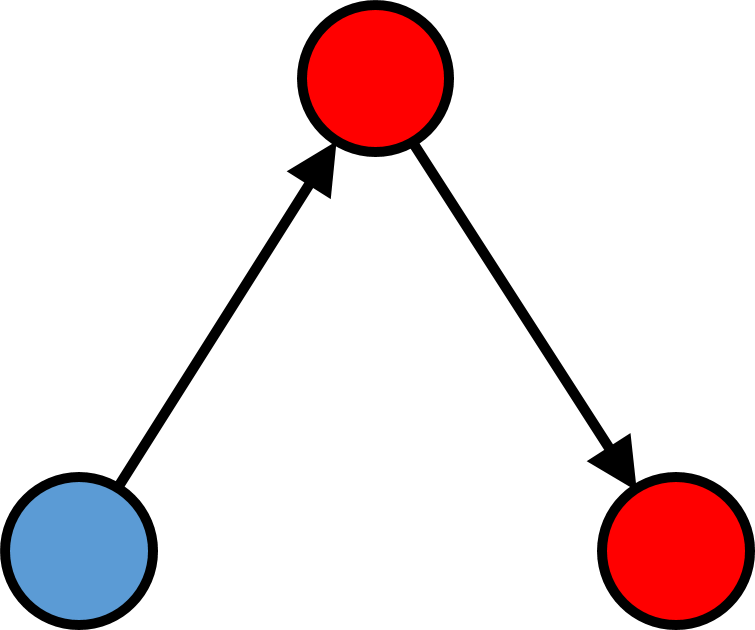
\includegraphics[width=\textwidth]{Images/b_OI.png}
    \caption{Gatekeeper}
    \label{fig:2}
  \end{subfigure}
  \hspace{2em}
  \begin{subfigure}[b]{0.25\textwidth}
    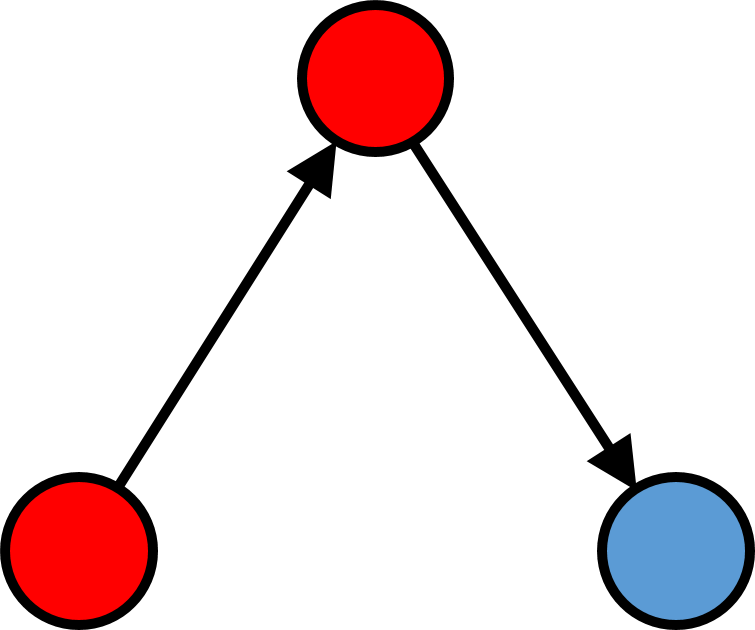
\includegraphics[width=\textwidth]{Images/b_IO.png}
    \caption{Representative}
    \label{fig:3}
  \end{subfigure}
  \par \bigskip
  \begin{subfigure}[b]{0.25\textwidth}
    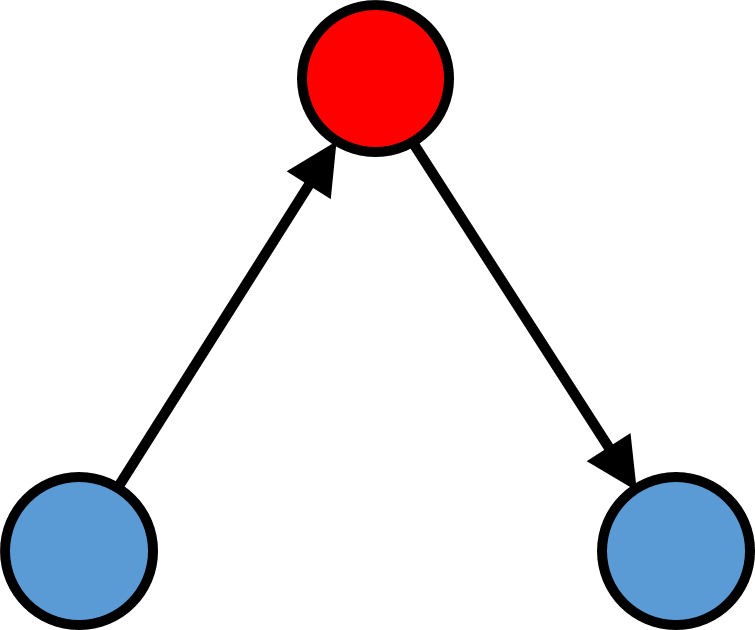
\includegraphics[width=\textwidth]{Images/w_O.png}
    \caption{Mediator}
    \label{fig:4}
  \end{subfigure}
  \hspace{2em}
  \begin{subfigure}[b]{0.25\textwidth}
    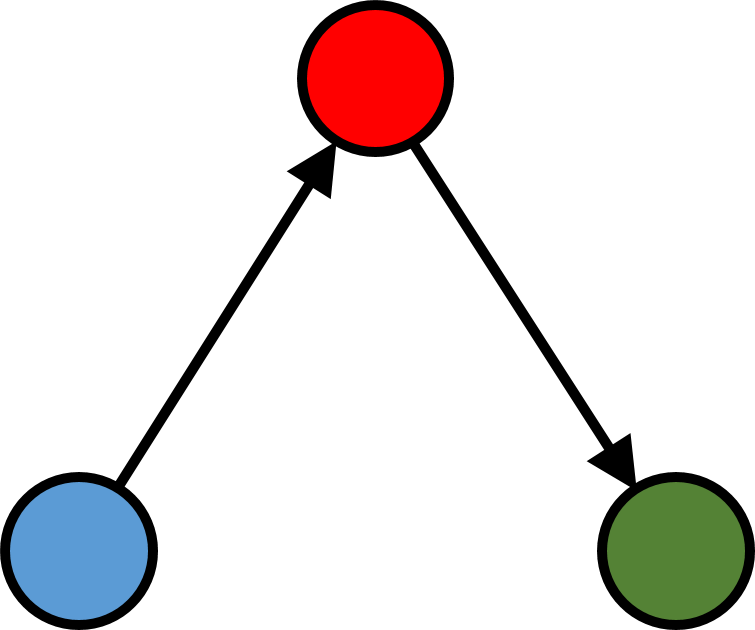
\includegraphics[width=\textwidth]{Images/b_O.png}
    \caption{Liaison}
    \label{fig:5}
  \end{subfigure}
  \caption[Broker roles]{\citet{gould1989structures} broker roles. The broker is the person receiving and sending ties. Colours represent different group affiliations.}%
    \label{fig:gf_roles}%
\end{figure}

Wrapping up, brokers play a vital role in establishing and growing knowledge networks. They are instrumental in identifying valuable sources of knowledge and connecting people who need knowledge with those who have it. Brokers also help others understand unfamiliar knowledge. From a structural perspective, brokers can use their position to their advantage (tertius gaudens brokerage). From a practice perspective, brokers oversee collaborative efforts to integrate and synthesise knowledge to obtain both individual and mutual benefit (tertius inungens and conduit brokerage). Hence, \bigskip  

\begin{tcolorbox}
\textit{\textbf{Proposition 2a:} Successful open innovation requires a combination of skilled brokerage and network closure (Research Question 2).}
\end{tcolorbox}

\section{Summary}

Conceptualising an open innovation partnership as a temporary knowledge network allows one to use social network analysis to assess knowledge sharing practices in meaningful ways. The value that can be extracted from the knowledge network depends on the absorptive capacity of partners. Whereas experiential knowledge is a vital component of absorptive capacity, applying knowing in practice also builds absorptive capacity. Applying knowing in practice requires good quality relationships. Brokers not only facilitate access to diverse sources of knowledge and expertise, they also can help others make sense of unfamiliar knowledge. Brokers occupy powerful positions as they are able to control access to knowledge. However, they also can empower others by giving them access to knowledge. Patterns of brokerage can reveal much about power relations in open innovation partnerships. \medskip

Agency refers to the capacity possessed by people to act of their own volition within an existing social environment   \citep{bandura1989human,emirbayer1998agency}. As agency lies at the heart of tacit knowledge exchange, the next chapter explores how motivation, trust, and power affect agency in open innovation partnerships.

\chapter{Motivation, trust, and power}
\section{Introduction}

This thesis employs a mixed-methods approach based on critical realism to examine the social mechanisms that shape tacit knowledge sharing in three open innovation partnerships. It characterises an open innovation partnership as a temporary knowledge network and assumes that human agency lies at the heart of tacit knowledge sharing. Autonomous motivation, the disposition to trust, and power relations in various social contexts influence an individual's decision to share or seek out tacit knowledge. We can use social network analysis to evaluate the interaction between agency and structure in open innovation partnerships and how this shapes tacit knowledge sharing behaviour. \medskip

This chapter explains the methodology used to assess the propositions developed in Chapter 2 across three open innovation partnerships. It includes justifications for embracing a critical realist worldview and employing a case-based mixed-method research design. The chapter details the quantitative and qualitative procedures used to collect and analyse data and the critical realist process used to interpret the data. 

\section{Research design}

\subsection{Research paradigm}

A research paradigm describes a worldview informed by philosophical assumptions about the nature of reality (ontology -- what do we believe about the nature of reality?), ways of knowing (epistemology -- how do we know what we know?), and ethics and value systems (axiology -- what do we believe is true?). We may treat ontology in terms of one verifiable reality or as multiple socially-constructed realities \citep{chilisa2012selecting}. Epistemology considers the nature of knowledge (versus the nature of reality) and involves asking questions about the sources of knowledge, the reliability of these sources, the extent to which we can we know about something, and how one can know if knowledge is real or not \citep{patton2002qualitative}. Methodology is where assumptions about the nature of reality, nature of knowledge, values, theory, and practice on a given topic come together \citep{chilisa2012selecting}.

\subsubsection{Positivist worldview}

Researchers studying the physical world tend to embrace a positivist paradigm, one that consists of a single tangible reality independent of cognition \citep{van2007engaged}. Positivists consider the scientific method as the only way to verify the existence of an objective reality \citep{creswell2011designing}. They see themselves as detached observers, able to reduce a problem into measurable parts, and demonstrate causality through statistical and mathematical methods \citep{easterby2015management}. Some argue that no matter how faithfully a researcher adheres to the scientific method, research outcomes are neither totally objective nor unquestionably absolute \citep[][p. 40]{crotty1998foundations}. The post-positivist paradigm accounts for bias and uncertainty by establishing causality through deductive falsification, unlike positivism which relies on inductive verification to generalise facts \citep{van2007engaged,chilisa2012selecting}. Efforts to ground social science in empirical investigations has led it to embrace a strongly positivist paradigm. By focusing more on epistemology than on ontology, social science has focused too much on methods and forms of explanation. Insufficient attention has been given to questions about what kind of entities actually exist in the social world and what are they like \citep{archer2016what}. 

\subsubsection{Constructivist worldview}

The constructivist paradigm assumes that reality is what people perceive it to be. Knowledge is considered to be subjective because it is socially constructed and dependent on personal beliefs and values \citep{chilisa2012selecting}. Since meaning is considered to exist within the human experience, the goal of constructivist research is to understand individual experiences. There is no preferred epistemology since discourses vary and are often incommensurable, and the research methodology reflects the assumptions of the researcher in attempting to interpret human experiences \citep{van2007engaged}. 

\subsubsection{Critical realist worldview}

In critical realism, reality is stratified into three ontological levels (see Figure \ref{fig:stratified_reality}). The first is the \enquote{empirical} level, which refers to aspects of reality observed or experienced directly or indirectly otherwise described as the transitive level of reality where events occur \citep{fletcher2017applying}. The second level consists of the \enquote{actual}, which refers to aspects of reality that may exist but are not necessarily observed or experienced \citep{mcevoy2006critical}. Events happen regardless of whether we experience or interpret them. Finally, the third level is the \enquote{real} and refers to the structures and mechanisms that cause or influence events \citep{zachariadis2013methodological}. These structures and mechanisms are beyond the realm of human observation and experience. They cannot be known or perceived and must be inferred through deductive (empirical investigation) and inductive (theory construction) processes \citep{mcevoy2006critical,wynn2012principles}. \medskip

\begin{figure}
\centering
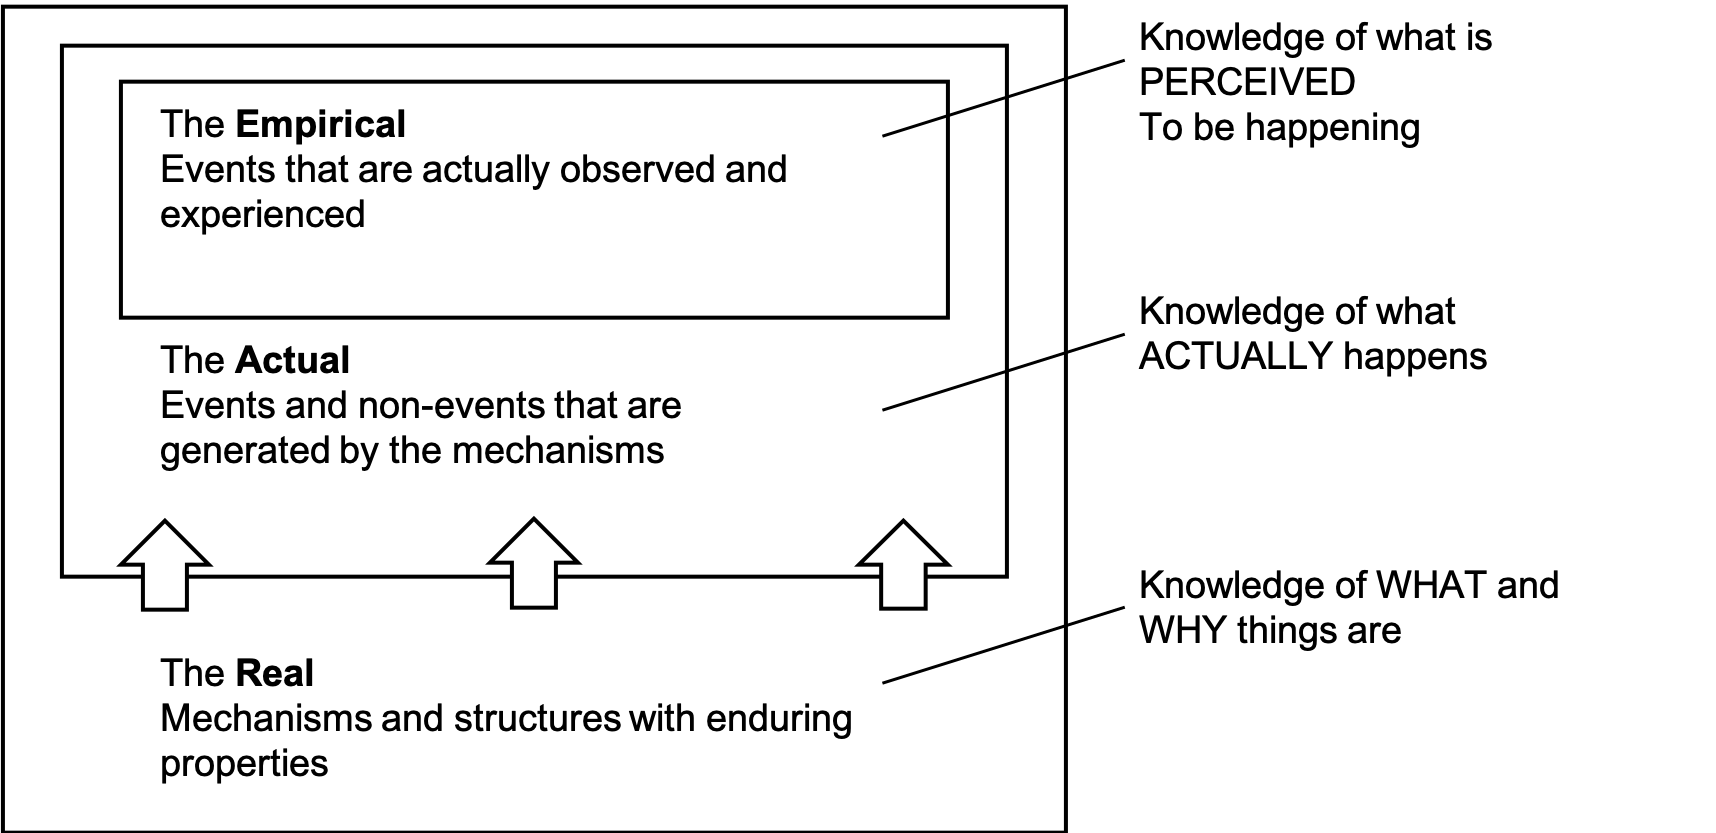
\includegraphics[width=0.9\linewidth]{Images/stratified_reality.png}
\caption[The stratified ontology of critical realism]{The stratified ontology of critical realism \citep{bhaskar2013realist,mingers2006realising}.}
\label{fig:stratified_reality}
\end{figure}

The critical realist uses the logic of retroduction to discover interacting mechanisms and structures that may explain events \citep{sayer1999realism,wynn2012principles}. Retroduction suggests new ideas or explanations, some of which may, after testing by induction, turn out to be true (Figure \ref{fig:retroduction}). These mechanisms or structures can be physical, social, or psychological and may not be directly observable except in terms of their effects (e.g. the configuration of network structures) \citep{mcavoy2018critical}. When dealing with multiple cases, the critical realist uses the logic of retrodiction to highlight differences between cases and merge different causal frameworks to develop a more general explanation of the mechanisms and structures that explain events \citep{welch2011theorising,mcavoy2018critical}.

Essentially, the primary goal of critical realism is to explain events through reference to these structures and mechanisms and the effects they can have across all three levels of reality \citep{wynn2012principles,fletcher2017applying}. \medskip

\begin{figure}[h!]
\centering
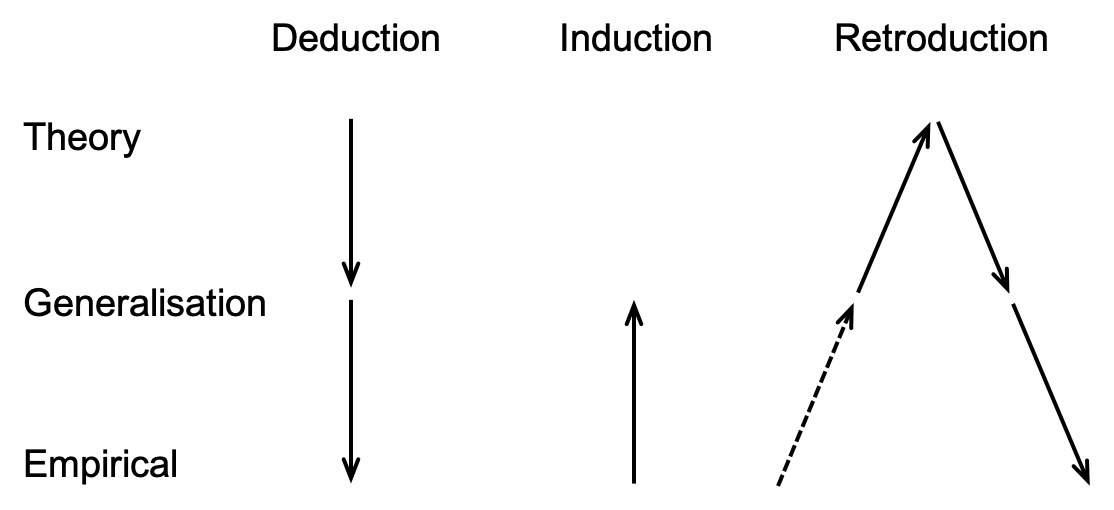
\includegraphics[width=0.7\linewidth]{Images/retroduction.png}
\caption[Logic of deduction, induction and retroduction]{Logic of deduction, induction and retroduction. Deduction is typically used to prove or disprove theory. Induction is used to generalise human experiences. Retroduction combines inductive and deductive reasoning to understand causal mechanisms as objectively as possible \citep{saether1998retroduction}.}
\label{fig:retroduction}
\end{figure}

\subsection{Justification for a critical realist approach}

This thesis aims to investigate mechanisms and structures that affect tacit knowledge sharing in open innovation. Though we can quantify social ties between participants and test hypotheses about tie formation in a positivist manner, this cannot account for external or experiential factors that influence tie formation. We need a combination of quantitative and qualitative methods to obtain a complete understanding of the mechanisms and structures affecting tacit knowledge sharing in open innovation. \medskip

Combining quantitative and qualitative methods is fraught because of the complex ontological and epistemological issues involved \citep{giddings2006mixed,mcevoy2006critical}. Methodological purists tend to be absolutist and argue strongly in favour of their preferred methodology. For them, quantitative and qualitative methods rely on mutually exclusive assumptions and are thus incommensurable \citep{greene2008mixed}. Methodological pragmatists, on the other hand, accept that assumptions can be mutually exclusive but assert that researchers should use whatever methods are needed to obtain useful results, even though this involves alternating between paradigms. The logic of methodological pragmatists is that neither quantitative nor qualitative methods alone are sufficient to develop a complete analysis \citep{mcevoy2006critical,creswell2013research}. Applying a pragmatic approach can be very challenging, especially when attempting to make sense of discordant data collected under different epistemological assumptions \citep{johnson2004mixed,giddings2006mixed}. Any study that involves mixing methods must reconcile ontological and epistemological differences to ensure findings are both credible and valid \citep{zachariadis2013methodological}. \medskip

The stratified ontology of critical realism allows for the \underline{legitimate} combination of qualitative and quantitative methods. Table \ref{tab:mm_critical_realism} lists reasons for mixing methods in critical realism. In the case of this study, the quantitative analysis tested psychosocial theories to explain significant network effects. The quantitative analysis was \underline{complemented} by qualitative analysis of semi-structured interviews, which allowed deeper exploration of the mechanisms and structures affecting tacit knowledge sharing in open innovation partnerships. Applying the logic of retroduction provided a more \underline{complete}, \underline{expansive} and \underline{diverse} picture of the mechanisms and structures affecting tacit knowledge sharing. 

\begin{sidewaystable}[p]
\centering
\resizebox{0.9\textwidth}{!}{%	
\begin{threeparttable}
\footnotesize
\setlength{\tabcolsep}{6pt}
\renewcommand{\arraystretch}{1}
\caption[Reasons for mixing methods in critical realism]{Reasons for mixing methods in critical realism \citep{zachariadis2013methodological}.}
\label{tab:mm_critical_realism}
\begin{tabular}{p{4cm}p{8cm}p{8cm}}
\toprule
\multicolumn{1}{c}{\textbf{Goal}} & \multicolumn{1}{c}{\textbf{Description}} & \multicolumn{1}{c}{\textbf{Critical realist implication}} \\ \midrule
Complementarity & Mixed methods are used in order to gain complementary views about the same phenomena or events & Different levels of abstraction of a multi\hyp{}layered world demand different methods \\
Completeness & Mixed methods research design is used to ensure a complete picture (as detailed as possible) of the phenomenon under study & Requires meta-theoretical considerations \\
Developmental & Inferences of one type of research are being used as questions for another type of research & This being part of the retroductive approach of critical realism, inferences need to hypothesise about the causal mechanisms whose recovery will then inspire additional research \\
Expansion & Mixed methods are being implemented in order to provide explanations or expand the understanding obtained in previous research & Quantitative methods can be used to guide qualitative research which (subject to the context) is more capable of uncovering generative mechanisms \\
Confirmation & Mixed methods are used in order to confirm the findings from another study & Epistemic fallacy occurs when trying to validate qualitative results with quantitative methods \\
Compensation & The weakness of one method can be compensated by the use of another & The weaknesses of different methods are recognised so alternative methods can be used to compensate \\
Diversity & Mixed methods are used in order to obtain divergent views on the same phenomena & Different levels of abstraction of a multi- layered world demand different methods \\ \bottomrule
\end{tabular}\end{threeparttable}
%
}
\end{sidewaystable}

\subsection{Case-based research}

A case study involves detailed examination of a particular case or set of cases within a real-world context \citep{crowe2011case}. It is an established research design used extensively in a wide variety of disciplines. The case study approach lends itself well to capturing information on more explanatory \textquote{how}, \textquote{what} and \textquote{why} questions \citep{crowe2011case}. How one approaches a case study depends on one's epistemological standpoint. For example, \citet{eisenhardt1989building} argues that case studies are a good way to develop social theories. She advocates inductive theory-building research to highlight associations between constructs and variables that can be tested. Her approach seeks to establish regularities rather than the reasons behind them i.e. it emphasises generalisation over context \citep{welch2011theorising}. \citet{yin2009case}, on the other hand, prefers a more deductive approach to case studies. He thinks case studies are well suited to test the validity of existing theories. His approach discounts contextual factors that may affect causal relationships \citep{welch2011theorising}. \citet{stake2005qualitative} argues that generalising the results of case studies is too simplistic and deterministic. He thinks the true value of case studies lies in understanding the uniqueness of each case. For him, it is all about understanding different contexts. \citet{welch2011theorising} argue that a critical realist approach offers a high degree of contextualisation without sacrificing the goal of causal explanation. Contextualised explanations can provide novel theoretical accounts that incorporate rather than deny complexity \citep{ragin2009reflections}. Table \ref{tab:welch_cases} highlights how the different case study approaches differ. \medskip

\begin{sidewaystable}
\centering
\caption[Case study paradigms]{Case study paradigms. After \citet{welch2011theorising}.}
\label{tab:welch_cases}
\resizebox{\textwidth}{!}{%
\begin{tabular}{@{}p{5.5cm}p{5.5cm}p{5.5cm}p{5.5cm}p{5.5cm}@{}}
\toprule
Dimension &
  Inductive theory building &
  Natural experiment &
  Interpretive sense-making &
  Contextualised explanation \\ \midrule
Philosophical orientation &
  Positivist (empiricism) &
  Positivist (falsification) &
  Interpretive/constructionist &
  Critical realist \\
Nature of research process &
  Objective search for generalities &
  Objective search for causes &
  Subjective search for meaning &
  Subjective search for causes \\
Case study outcome &
  Explanation in the form of testable propositions &
  Explanation in the form of cause and effect linkages &
  Understanding of actor's subjective experiences &
  Explanation in the form of causal mechanisms \\
Strength of case study &
  Induction &
  Internal validity &
  Rich description &
  Causes-of-effects explanations \\
Attitude to generalisation &
  Generalisation to population &
  Generalisation to theory (analytic generalisation) &
  Particularisation not generalisation &
  Contingent and limited generalisations \\
Nature of causality &
  Regularity model: proposing associations between events (weak form of causality) &
  Specifying cause effect relationships (strong form of causality) &
  Too simplistic and deterministic a concept &
  Specifying causal mechanisms and the contextual conditions under which they work (strong form of causality) \\
Treatment of context &
  Contextual description a first step only &
  Causal relationships are isolated from the context of the case &
  Contextual description necessary for understanding &
  Context integrated into explanation \\
Primary advocate &
  \citet{eisenhardt1989building} &
  \citet{yin2009case} &
  \citet{stake2005qualitative} &
  \citet{ragin2009reflections,bhaskar2013realist} \\ \bottomrule
\end{tabular}%
}
\end{sidewaystable}

\subsection{Mixed-methods research design}

This thesis uses a case-based mixed-method research design to unpack the social mechanisms and structures that shape tacit knowledge exchange ties in three open innovation partnerships. Figure \ref{fig:mm} outlines the different research stages of this study. The first step identified research gaps in the open innovation literature. These informed the research questions that are the focus of this study. The next step was to apply a critical realist research process to identify critical social mechanisms affecting tacit knowledge exchanges in open innovation partnerships, their impact, and how these are activated \citep{mcavoy2018critical}. \medskip

\begin{figure}[p]
\centering
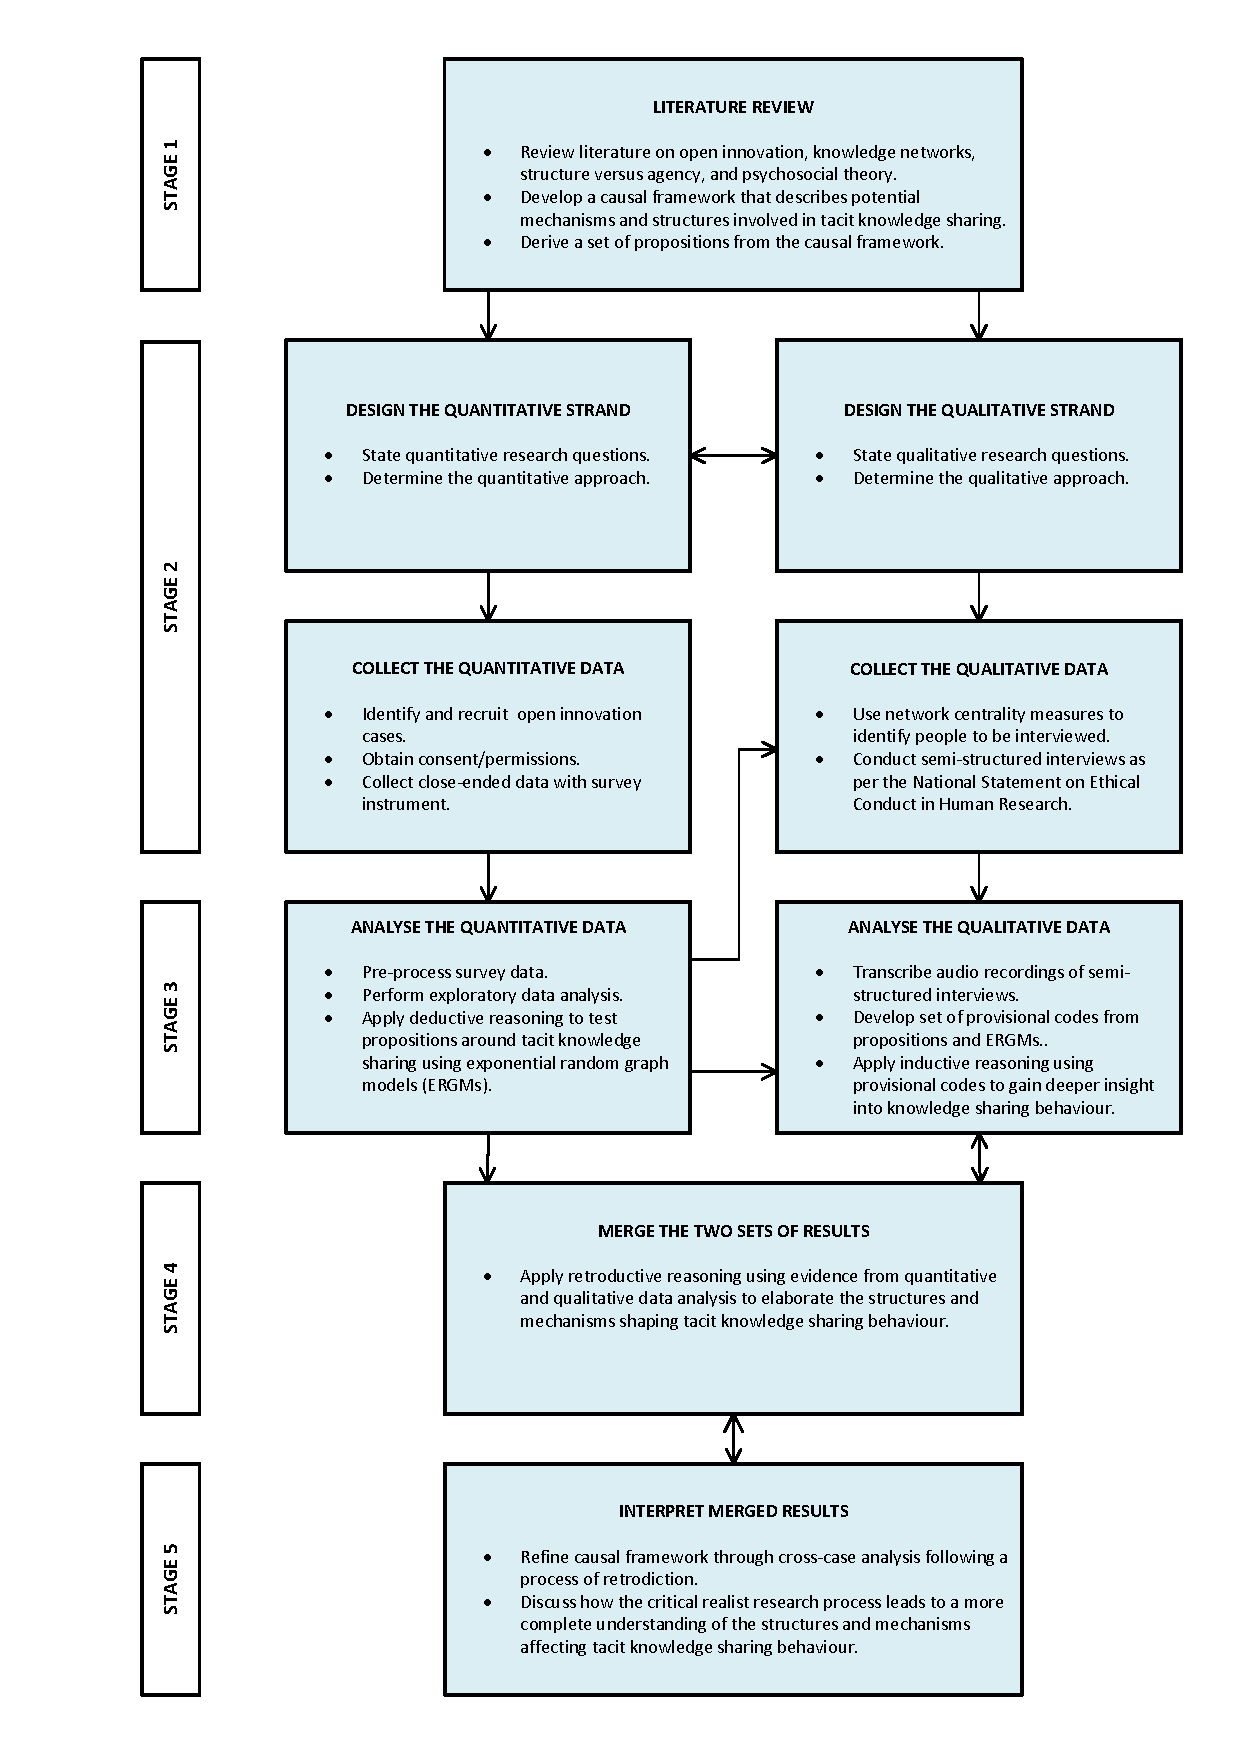
\includegraphics[width = 1.0\textwidth]{Images/mm.pdf}
\caption[Mixed-method research design]{Mixed-method critical realist research design.}
\label{fig:mm}
\end{figure}

Determining causal mechanisms in social network analysis is difficult because of the confounding nature of endogenous and exogenous network effects \citep{rogowski2012estimating,forastiere2018estimating}. Exponential random graph models (ERGMs) are a class of statistical model for social networks that allow simultaneous testing of multiple hypotheses about network structure and tie formation. Models represent an accumulation of local network configurations (also referred to as subgraphs, motifs, or microstructures) that build the global structure of the network \citep{robins2013tutorial}. Network configurations are assumed to represent underlying social processes or mechanisms \citep{lusher2013exponential}. A combination of social and psychological theories was used to predict purely structural network effects (reciprocity, popularity and activity spread, simple as well as multiple connectivity, transitive closure), actor-relation effects (sender/receiver, homophily), and actor-brokerage effects (different broker roles). While such quantitative analysis can disambiguate potentially confounding network effects, it cannot account for unobserved contextual or experiential factors that may affect network structures in open innovation partnerships. Hence, the next step in the critical realist research process is to apply retroduction to develop a more robust causal framework for each case. In the case of this study, the process of retroduction relied on evidence from the exponential random graph models and semi-structured interviews. It is important to note that with cross-sectional studies, such as this one, there is a limit to what one can infer about causal mechanisms. \medskip

The final step in the critical realist research process involves combining the causal frameworks for each case to create a cross\hyp{}case causal framework. Differences between cases are reconciled using retrodiction to create more robust explanations of mechanisms \citep{mcavoy2018critical}. \medskip

\section{Ethics clearance}

As this thesis deals with human participants, it was subject to the ethical guidelines contained in the Australian National Statement on Ethical Conduct in Human Research \citep{national2014national}. Formal ethics approval from both the Commonwealth Scientific and Industrial Research Organisation and Swinburne University of Technology was required before any data could be collected. Approval hinged on individual participants being sufficiently informed to give consent, allowing information about themselves to be used in this study. An application for ethics clearance was submitted to the ethics committees at both organisations. The application included a brief description of this study, a plain language information sheet for participants, a blank consent form, and a list of questions to be included in an online survey. Both committees deemed this study low-risk and allowed the collection and subsequent analysis of data to proceed, subject to standard terms and conditions as per the National Statement on Ethical Conduct in Human Research (the ethics approval may be found in Appendix A). These include alerting both committees to any changes in data collection procedures and reporting any complaints or issues raised by participants. None of the study participants raised any issues with the conduct of this study. 

\section{Research participants}

Finding appropriate candidates for open innovation case studies was challenging. This thesis is part of a broader initiative looking at innovation in the food and agriculture sector. Potential candidates were identified using leads provided by agricultural consultants, university researchers, government agencies, and non-governmental organisations. Most of the firms approached were not that keen on outsiders observing how they went about open innovation. Some firms argued that their inter-organisational relationships were trade-secrets and did not want to risk anyone finding out about their strategic or commercial intentions. Other firms felt this study would consume too much their time or be too disruptive to their operations. Ultimately, the recruitment of cases relied on a combination of perseverance and goodwill. Altogether three cases were recruited for this study. 

\section{Quantitative procedures}

\subsection{Data collection}

Each case followed the same procedure for collecting and analysing quantitative data. For each case, the primary contact person (usually the project instigator) was asked to compile a list of people directly involved in the effort. An online survey was employed to collect quantitative data. The survey captured demographic information about respondents, whom they related to in the collaboration, and how they perceive themselves.\medskip

Any missing data impacts negatively on network studies. Hence this study aimed for a 100\% survey response rate. The primary contact person was asked to strongly encourage everybody on their list to participate in this study. 

\subsubsection{Questionnaire design}

The online survey was kept short as an inducement to complete the survey and to avoid responder fatigue \citep{crawford2001web,evans2005value,van2006conducting}. An informal poll among workplace colleagues at the Commonwealth Scientific Industrial Research Organisation (CSIRO) indicated that an online survey should take no longer than 15 or so minutes to complete. With this limitation in mind, the survey questionnaire was designed with three parts. The first part captured demographic information about the respondent, namely their age, gender, occupation, level and field of education, workplace postcode, relevant work experience, and current job tenure. Relevant work experience is essential as this is the primary source of useful tacit knowledge \citep{nonaka1995knowledge,sternberg1999tacit}. Response options for categorical questions were based on the Australian and New Zealand Standard Classification of Occupations \citep{pink2009anzsco} and the Australian Standard Classification of Education \citep{trewin2000australian}. Respondents were also asked to state their role in the open innovation partnership. \medskip

The second part of the questionnaire captured information about specific social relationships. Respondents were asked to name people in the open innovation collaboration they received knowledge and ideas from, felt they could trust, who they reported to, and have worked with before (see Table \ref{tab:ng} for list of the name-generator and name-interpreter questions). \bigskip

\begin{table}[p]
\centering
\caption[Name-generator/interpreter questions]{Name-generator (NG) and name-interpreter (NI) questions.}
\label{tab:ng}
\begin{tcolorbox}
\begin{itemize}
\item[\textbf{NG 1}] \textit{Name people who provide you with useful knowledge that helps you accomplish your tasks in this collaboration.}
\begin{itemize}
\item[\textbf{NI 1-1}] \textit{How much of the knowledge provided by this person is documented?}
\item[\textbf{NI 1-2}] \textit{How complex is the knowledge provided by this person?}
\item[\textbf{NI 1-3}] \textit{How much time does this person spend demonstrating their knowledge to me?}
\end{itemize}
\item[\textbf{NG 2}] \textit{Name people who help you come up with new ideas or novel solutions to hard problems in this collaboration.}
\item[\textbf{NG 3}] \textit{Name people who help you transform ideas into product, process or service concepts for further development and commercialisation in this collaboration.}
\item[\textbf{NG 4}] \textit{Name people in the collaboration you can share ideas, feelings and hopes with. These are people with whom you have made a considerable emotional investment in your working relationship. You can talk freely with them about the difficulties you are having at work. They will listen and respond in a constructive, caring way. You would share a sense of loss with them if you could no longer work together.}
\item[\textbf{NG 5}] \textit{Name people in the collaboration you consider professional, competent, and dedicated. You can count on them not to make your job harder by careless work. They have the trust and respect of their colleagues, including those who are not friends.} 
\item[\textbf{NG 6}] \textit{Name people you formally report to in this collaboration.}
\item[\textbf{NG 7}] \textit{Name people in this collaboration you have worked and interacted with prior to this collaboration getting underway.}
\end{itemize}
\end{tcolorbox}
\end{table}

Respondents could select names from a drop-down list or add names of people missing from the list. Asking respondents whom they receive knowledge and ideas from, rather than whom they share knowledge or generate ideas with, was a deliberate move to avoid them nominating everybody in the drop\hyp{}down list. Asking respondents to nominate whom they received knowledge and ideas from required them to think more carefully about their response. Respondents also had to indicate how much of the knowledge provided to them was tacit. Tacit knowledge may be characterised in terms of \enquote{complexity}, \enquote{codifiability}, and \enquote{observability} \citep{winter1987knowledge,zander1995knowledge,cavusgil2003tacit}. Any knowledge that is complex, poorly encoded, and mostly acquired through observation is considered to be predominantly tacit. For each knowledge provider, respondents had to rate the complexity of the knowledge provided to them, the extent to which the knowledge was documented, and how much direct observation was required to obtain the knowledge on a 10\hyp{}point scale. \medskip 
The third part of the questionnaire aimed to build a psychological profile of the respondent in terms of personality, self-efficacy, organisational identification, and work motivation. Respondents had to rate their level of agreement with several statements about themselves, using a 10-point scale. Items from an ultra-shortened version of the \enquote{Big Five Inventory} was used to profile personality. The BFI-10 scale uses two items to measure each of the big five personality traits \citep{rammstedt2007measuring}. Only three personality traits positively correlated with knowledge sharing were profiled, namely \enquote{agreeableness}, \enquote{conscientiousness}, and \enquote{openness to experience} \citep{matzler2008personality,matzler2011personality}. While the BFI-10 is reported to be a less reliable scale (agreeableness: $\alpha$ = 0.42, conscientiousness: $\alpha$ = 0.67, emotional stability: $\alpha$ = 0.78, extraversion: $\alpha$ = 0.79, openness: $\alpha$ = 0.50), it is sufficient for research settings with tight time constraints, such as this study \citep{rammstedt2007measuring}. \medskip

This study assessed self-efficacy in terms of how competent a person felt about doing their job, their sense of autonomy, and confidence in their ability to come up with creative ideas or solutions. Job competence and autonomy was profiled using selected statements from the \enquote{Measuring Empowerment Scale} \citep{spreitzer1995psychological}. Reported reliability of this scale is considered good (job competence: $\alpha$ = 0.81, self-determination: $\alpha$ = 0.81). The ability to come up with creative ideas or solutions was profiled using statements from the \enquote{Creative Self\hyp{}Efficacy Scale} \citep{tierney2002creative}. Past studies indicate that this scale is reliable with reported $\alpha$ values between 0.74 and 0.91 \citep{tierney2002creative,gong2009employee,tierney2011creative,mittal2015transformational}. \medskip

The \enquote{Organisational Identification Scale} \citep{mael1992alumni} was used to assess how strongly the respondent identified with his or her work\hyp{}group, employer, and with the open innovation partnership. This scale has proved to be reliable in a variety of study settings with reported $\alpha$ values between 0.73 and 0.89 \citep{mael1992alumni,bergami2000self,knippenberg2000foci,van2008interactive}. Only one of the six items from the scale was used in this survey: \enquote{When someone criticises my organisation, it feels like an insult}. This item has the highest factor loading of all six items \citep{mael1992identifying} and was adapted to address identification with one's workgroup, with one's employer, and with the partnership. Using all six items for each of these cases would have been impractical, given the time constraint in which to complete the survey. \medskip

Work motivation was measured using all 19-items from the \enquote{Multidimensional Work Motivation Scale} \citep{gagne2015multidimensional}. This scale is based on self-determination theory and has sub-scales for amotivation, extrinsic material regulation, extrinsic social regulation, introjected regulation, identified regulation, and intrinsic motivation. Reliability of the English version is good, with reported $\alpha$ values between 0.79 and 0.90. Items in the Multidimensional Work Motivation Scale were modified to suit the study context. For example, the scale has a stem question: \enquote{Why do you or would you put efforts into your current job?}. One response option is: \enquote{Because I personally consider it important to put efforts into this job}. This response was modified to read as thus: \enquote{I put effort into this collaboration because I personally consider it important to do so}. 

\subsubsection{Piloting of the survey}

For quality assurance, the online survey was piloted twice to check if questions were clear and not ambiguous and to establish how long it would take to complete an online survey. Ten people were involved in each pilot (the first pilot involved CSIRO colleagues, the second involved members of the Social Network Research Laboratory at Swinburne University of Technology). Apart from one question about trust, everybody in the first pilot reported no issues with clarity or ambiguity. One person felt the question asking respondents to name people in the partnership they trust was too judgemental. The question was subsequently modified to be less judgemental. Everybody involved in the second pilot was comfortable with the survey, although one person felt the invitation email was too long. Most of the people in each pilot completed the survey within 20 minutes. The only exceptions were people who took their time making detailed notes as they went through the survey. Table \ref{tab:self-report} in Appendix B lists the 59 items used in the online survey, together with associated response options and references.

\subsubsection{Survey procedure}

The list of people involved in each open innovation partnership also included their email addresses. Everybody on the list received an email invite to complete the web-based survey questionnaire. The email provided information about the study and included a unique link to the survey website (\url{http://www.onasurveys.com}). People could either ignore the email invitation or agree to take part in the survey by clicking on the URL link provided. Clicking on the URL link directed them to the survey website where they were asked to give consent to allow their responses to be used in this study. They could not progress with the online survey until consent was given.

\subsection{Social network analysis}

\subsubsection{Key concepts}

A social network is a way to conceptualise a social system in terms of the structure of relationships among social actors. Typically, a social network is represented as a mathematical graph with vertices and edges. Vertices represent actors (also referred to as nodes) and edges the ties (social connections or relations) between them (Figure \ref{fig:examples}). \medskip

\begin{figure}
    \centering
    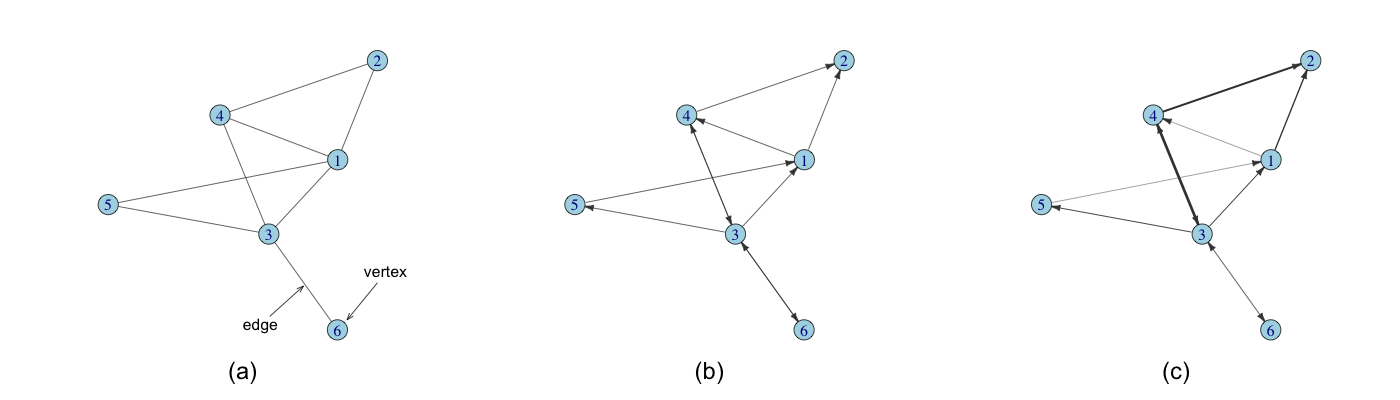
\includegraphics[width=1.0\linewidth]{Images/example_networks.png}
    \caption[Example networks]{Example network with (a) undirected binary ties, (b) directed binary ties, and (c) valued ties (edges are weighted according to some value).}
    \label{fig:examples}
\end{figure}

Actors may be distinguished using any combination of binary, categorical or continuous attributes. For example, consider an individual actor classified as female (binary attribute), who works for a particular organisation (categorical attribute), with a specific number of years of work experience (continuous attribute). Ties between actors can be measured as directed or undirected, and as binary or valued. Deciding whether to measure a tie as directed or undirected depends on the nature of the tie. For instance, ties indicating organisational affiliation are usually undirected, whereas authority is inherently directed \citep{borgatti2013analyzing}. \medskip
 
 A similarity tie is a type of continuous tie that shows a relation between two actors who share something in common (e.g. work at the same location, are affiliated to the same body, participate in the same event, or share a common attribute). Actors can have many different kinds of social relations, e.g. friendship, knowledge sharing, advice seeking, and reporting ties. Relational ties can also be affective (like or dislike another actor) or perceptual (belief about the other actor). Discrete ties refer to ties defined by specific social interactions (e.g. a transaction of some kind, attendance at the same event) and flows (e.g. communication or knowledge flows). \medskip

Ties are often interdependent insofar as the presence of one tie affects the presence of others. Without some form of dependence among ties, it is often difficult to explain the existence of specific social relations \citep{lusher2013exponential}. An example is a friendship tie, which usually develops in the presence of a pre-existing similarity tie and vice versa (e.g. both actors share a common interest or work at the same place) or via an interaction tie (e.g. actors were introduced to each other at a specific event or worked together on a particular project). \medskip

\begin{figure}
    \centering
    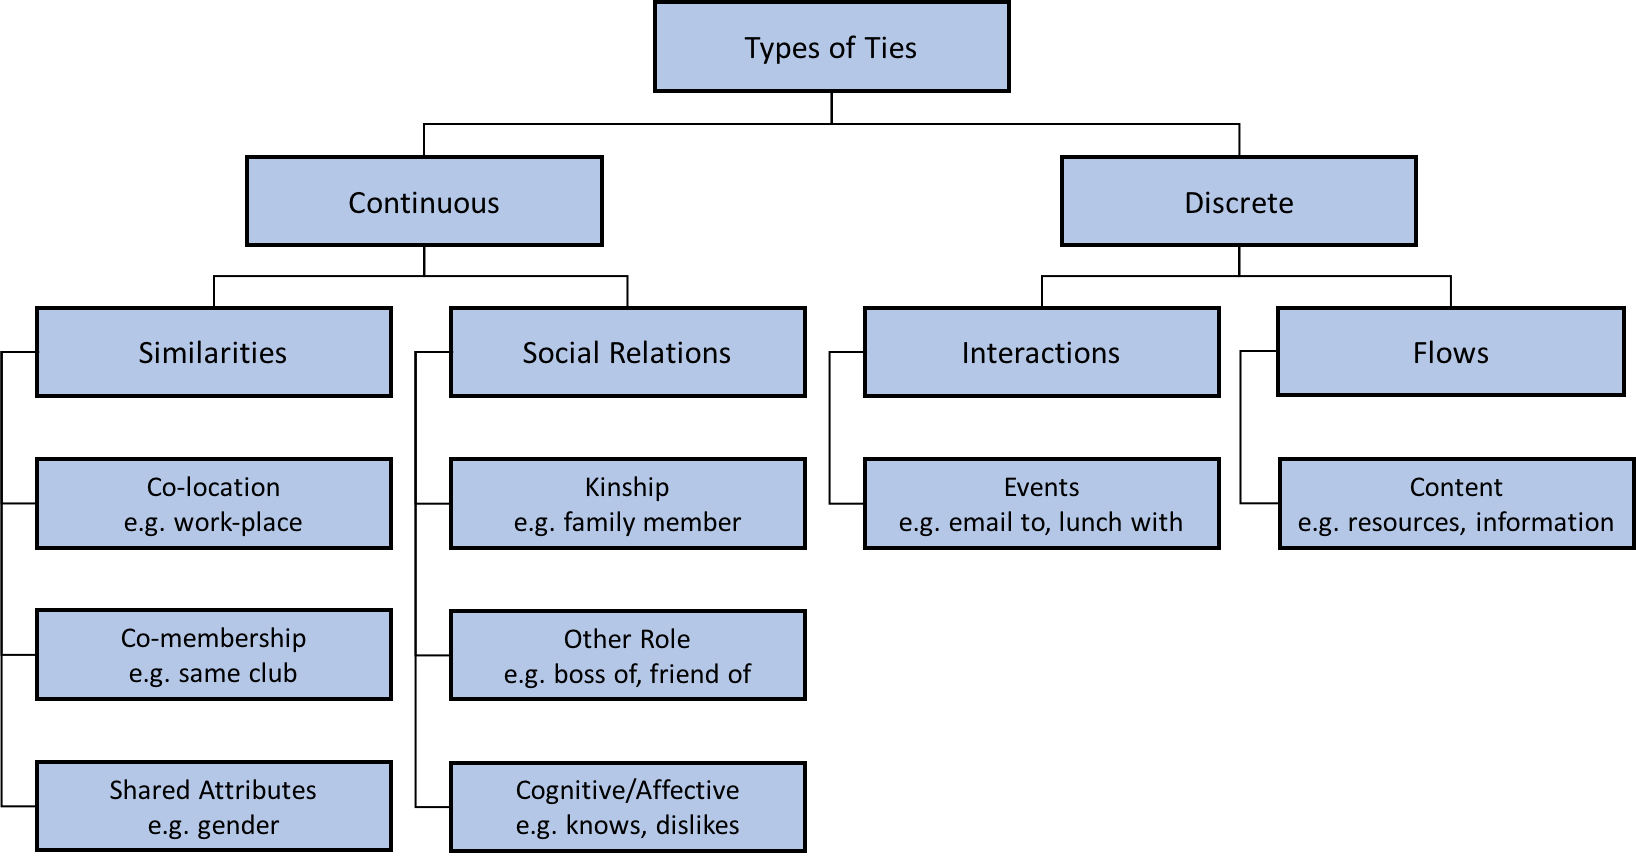
\includegraphics[width=0.9\linewidth]{tie_type}
    \caption[Different types of social ties]{Different types of social ties \citep{borgatti2013analyzing}.}
    \label{fig:tie_type}
\end{figure}

\subsubsection{Network data structures}

Edge lists and adjacency matrices are the most commonly used data structures for social networks. With an edge list, an edge between two actors $i$ and $j$ is denoted as $(i,j)$, so that a complete network with $n$ actors can be specified by giving the value $n$ and a list of edges. The edge list for the undirected binary network depicted in Figure \ref{fig:examples} would have $n = 6$ actors and edges (1,2), (1,3), (1,4), (1,5), (2,4), (3,4), (3,5), (3,6). A directed network has twice the number of total possible edges than an undirected network (directed network edges can be bi-directional). Thus, the edge list for the directed binary network depicted in Figure \ref{fig:examples} would have $n = 6$ actors and edges (1,2), (1,4), (3,1), (3,4), (3,5), (3,6), (4,2), (4,3), (5,1), (6,3). Although edge lists are an efficient way to represent networks, they are too cumbersome for computational operations \citep{newman2010networks}. \medskip

An adjacency matrix is a more efficient way to represent and manipulate social network data \citep{hummon1990computational}. For a social network, $X$, the adjacency matrix would be a $n \times n$ matrix with elements $X_{ij}$ representing how actor $i$ is tied to actor $j$. In the case of a binary network, the adjacency matrix is expressed as follows: 
\[
X_{ij} =
\begin{cases}
    1 & \text{if  } i \rightarrow j \\
    0 & \text{otherwise}
\end{cases}
\]
For an undirected network, $X_{ij}$ and $X_{ji}$ are equal. With a directed network, $X_{ij}$ and $X_{ji}$ are treated as different variables, either with the same or different values. For a directed binary network, values = 1 in the $i$th row of an adjacency matrix represent ties sent by actor $i$, and the values = 1 in the $j$th column of an adjacency matrix represent ties received by actor $j$. The adjacency matrix representing both the directed and undirected binary networks depicted in Figure \ref{fig:examples} would be expressed as: \bigskip
$$
X_{ij} =
\left \{
  \begin{tabular}{cccccc}
    0 & 1 & 0 & 1 & 0 & 0 \\
    0 & 0 & 0 & 0 & 0 & 0 \\
    1 & 0 & 0 & 1 & 1 & 1 \\
    0 & 1 & 1 & 0 & 0 & 0 \\
    1 & 0 & 0 & 0 & 0 & 0 \\
    0 & 0 & 1 & 0 & 0 & 0
  \end{tabular}
\right \}
$$ \medskip

In the case of non-binary or valued networks, the presence of a tie is indicated by some value (usually a real number, not equal to 0) that describes a property of the tie, e.g. geographic proximity.

\subsubsection{Types of social network analysis}

Social network analysis aims to detect and interpret patterns of social ties between actors \citep{de2011exploratory}. According to \citet{knoke2008social}, three assumptions about patterned relations and their effects underpin social network analysis. First, structural relations are often more important than actor attributes for understanding social behaviour. For instance, an actor may be well-qualified to perform a specific task, but unable to do the task because the requisite relationships are not in place (i.e. the absence of of structure inhibits agency). Second, social networks shape and are shaped by the perceptions, beliefs, and actions of actors. Third, network structures are dynamic and continually evolving \citep{knoke2008social}. Social network analysis can be either egocentric or sociocentric. Egocentric network analysis focuses on the structure of an actor's immediate network (the ego's network) and what this means for that actor \citep{chung2005exploring}. In contrast, sociocentric network analysis considers patterns of social interaction between all the actors in a predefined and bounded population \citep{provan2007interorganizational}. \medskip

This thesis used both descriptive and statistical network analysis techniques to analyse the sociocentric network structure of the three open innovation partnerships. The descriptive network analysis measured the centrality of actors and their brokerage roles in each open innovation partnership. This information was used to identify a subset of actors for follow-up semi-structured interviews (the subset included highly central as well as peripheral actors). The statistical network analysis used exponential random graph models (ERGMs) to examine the interdependence of knowledge sharing ties.

\subsubsection{Brief history of ERGMs}

Traditional methods for analysing social networks are primarily descriptive and not statistical in the sense of modelling random variation in how ties are formed among actors in a network \citep{harris2013introduction}. \citet{erdos1959random} formulated a simple random graph in which the proportion of observed ties out of all possible ties determines the probability of a tie forming between two actors. Simple random graphs are not very good at capturing observed network structures as they do not account for the social forces that influence tie formation \citep{harris2013introduction}. This led \citet{holland1981exponential} to introduce a random graph model for directed graphs, where the probability of tie formation varies among actors according to their propensity to extend ties to other actors, and the propensity to have ties extended to them by other actors (referred to as a $p_1$ model). \medskip

While this was an improvement over simple random graphs, $p^1$ models do not reflect the interdependence among network ties or attributes of nodes (e.g. homophily and transitivity effects). Consequently, \citet{frank1986markov} introduced a new generation of random graph model that assumes a form of dyadic dependence when ties do have actors in common (the Markov dependence assumption). Although it incorporated more of the structural characteristics found in observed networks, the model introduced by \citet{frank1986markov} does not include node attributes as covariates. \medskip

A major breakthrough came when \citet{wasserman1996logit} introduced a new model that assumes a more general conditional dependence among ties. Essentially, this model assumes the likelihood of any two ties existing at the same time is different from the combined likelihood of each tie being present. Their model allows for multiple dependence assumptions at both dyadic and node level(hence these models are referred to as $p^*$ models). \medskip

Statistically, an ERGM represents a probability distribution of graphs for a given set, where the probability of observing a graph is dependent on the presence of the various network configurations expressed by the model. Importantly, the unit of analysis in an ERGM is not the number of nodes, but the number of possible ties between all actors in the network ($n(n-1)$ possible ties for directed, and half of that for non-directed networks). Even with a small number of actors, an ERGM has sufficient statistical power to make inferences about how ties are formed \citep{lusher2013exponential}. \medskip

For a binary network, the probability of observing specific network configurations for a given set of actors \(n\) can be expressed as follows: $$ P(X = x) = \frac{\exp \left \{ \theta'z(x)  \right \}}{\kappa (\theta )} $$ where $P(x)$ indicates the probability of a given network, $\theta$ indicates a vector of model parameters, $z(x)$ is a vector of network statistics, and $\kappa$ is a normalising function to ensure a proper probability distribution across a set of random networks \citep{shumate2010exponential}. Network statistics $z(x)$ are counts of local configurations in the network, or some function of those counts. The probability of the network depends on how many of those configurations are present and the parameters indicate the importance of each configuration \citep{lusher2013exponential}. Large positive parameters suggest that more configurations of that type are observed in the network than expected by chance alone \citep{robins2009closure}. \medskip

ERGMs are theory-driven in that their use requires the researcher to consider the complex, intersecting, and often competing theoretical reasons why particular social ties in the observed network exist \citep{lusher2020advances}. For instance, does a given network structure occur due to processes of homophily, reciprocity, transitivity, or through a combination of these? By including such parameters together in one model, a researcher can test certain hypotheses or propositions about tie formation relating to theory \citep{robins2007recent}. ERGMs can distinguish between ties formed due to actor attributes or whether an actor’s centrality is the result of being embedded within other purely structural network structures \citep{lusher2020advances}. Purely structural effects reflect self-organising or endogenous processes where ties form due to the presence or absence of other ties, e.g. reciprocity and transitive closure. Actor-relation effects refer to ties that form due to actor attributes. Homophily is an example of an actor-relation effect. Dyadic covariate effects refer to ties in one network being affected by ties in another network or other dyadic measurements. A good example is the geographic separation between actors, which may affect the formation of relationships between them. Another example is advice seeking, which is more likely to occur in the presence of an existing friendship tie. \medskip

Alternative methods used to assess the effect of actor attributes on network structures, such as linear regression, are unable to make such distinctions and are thus more limited regarding the conclusions such methods can draw. One limitation of ERGMs is that the algorithms used to estimate model parameters may fail to converge, especially for large networks (i.e. are unable to produce a stable set of parameter estimates that can capture the various graph statistics included in the model). For the cases presented in this thesis, all findings are based on converged ERGMs that provided adequate fit to the observed network data.

\subsubsection{Data pre-processing}

The first step was to retrieve survey responses for each case from the \texttt{ONASurveys} website. Each case had its own Microsoft Excel\texttrademark\ workbook with two worksheets. The first worksheet contained demographic information about each respondent and their responses to the personality, self-efficacy, organisational identification, and work motivation scale items. The second worksheet listed for each respondent their nominated sources of knowledge and ideas, people they work with to realise ideas, trusted others, line or project managers, and individuals with whom they have previously worked. \medskip

Various \texttt{R} packages were used to pre-process data for social network analysis, generate network diagrams, and perform descriptive network analysis. These are listed in Appendix C (Table \ref{tab:r_scripts}). \texttt{R} is a popular cross-platform open-source software system for statistical computing \citep{core2018r}. Readers can access the \texttt{R} scripts used to pre-process, analyse and visualise data at \url{http://github.com/aterhorst/phd_scripts}. The exponential random graph modelling was done using \texttt{MPNet}, a Microsoft Windows\texttrademark\ application for statistical network analysis \citep{wang2014mpnet}. \medskip

Survey responses were loaded into \texttt{RStudio}, a free and open-source integrated development environment (IDE) for \texttt{R}, as two separate tabular data sets (i.e. a node table listing personal information about each respondent, and an edge table listing the different ways respondents relate to each other). The first step in the data tidying process involved fixing minor data-entry errors in the node table. Once data-entry errors were eliminated, the next step involved aggregating the personality, self-efficacy, organisational identification, and work motivation scale items. Aggregated scale items were re-scaled to be a fractional number between 0 and 1. \medskip

Respondents had to qualify the type of knowledge provided to them in terms of its complexity, observability, and level of encoding \citep{winter1987knowledge,zander1995knowledge,cavusgil2003tacit}. Knowledge sharing relations were valued on a scale of 0 to 1 by aggregating and re-scaling the three criteria to come up with a measure of knowledge tacitness. This allowed knowledge sharing relations to be split into two types, i.e. predominantly tacit and predominantly explicit knowledge sharing relations. Predominantly tacit knowledge (tacitness $> 0.5$) lacks documentation, is likely to be complex, and is mostly acquired through observation. Predominantly explicit knowledge (tacitness $< 0.5$), on the other hand, tends to be well-documented, is not particularly complex, and requires little demonstration to be communicated. Although the edges of the predominantly tacit and a predominantly explicit knowledge network do not overlap, this thesis does not treat knowledge as a binary construct (as either completely tacit or totally explicit knowledge). This thesis assumes all knowledge has a tacit component. It uses a simple majority rule to differentiate knowledge according to its level of tacitness. In other words, the tacit and and explicit knowledge networks do not overlap. \medskip

A multilayer network object was generated from the cleaned node and edge data. Each layer in the network object represents a different set of relationships (tacit and explicit knowledge provider, idea contributor, cognition-based trust, affect-based trust, reporting, and historical relations). Given that the survey asked respondents to name people in the partnership who (a) provided them with useful knowledge, and (b) contributed ideas to help them solve problems, the edges in both the knowledge provider and idea contributor layers were reversed to indicate the flow of knowledge and ideas. \medskip

The survey questionnaire asked respondents to enter their workplace postcodes. Geographic coordinates (longitude and latitude) were derived for each postcode using the \texttt{ggmap} package (the \texttt{geocode} function uses the Google Maps\texttrademark\ application programming interface (API) to do this). The spherical (also known as the \enquote{great circle}) distance between all survey respondents could then be calculated using the \texttt{geosphere} package (distances were expressed in kilometres). This information was added as dyadic covariate (or edge attribute) in each network layer. \medskip

Adjacency matrices and corresponding node attributes were extracted from the multilayer network object and saved as ASCII text files for exponential random graph modelling in \texttt{MPNet}. Apart from the valued adjacency matrix representing geographic separation between nodes (values = $log_e(\text{spherical distance(km)} + 1)$ between nodes), the adjacency matrices were binary in nature (0 = no edge between nodes, 1 = edge between nodes). Using the natural log of the distance mad sense because we were dealing with a vast range of distances in each case. 

\subsubsection{Exploratory data analysis}

The first thing to do with any survey data set is to get to know it. Not only does this allow one to become familiar with the data, it also helps reduce the workload during analysis \citep{cox2017translating}. Exploratory data analysis is about finding trends in the data, not so much about the strength of the evidence \citep{morgenthaler2009exploratory}. Usually, this involves applying various data visualisation techniques to explore the content and structure of the survey data. Insights gained from exploratory data analysis can help refine research questions, strengthen hypotheses, and improve model specifications \citep{jebb2017exploratory}. \medskip

Exploratory data analysis was used to assess responses to the survey scale items, check for significant correlations between survey items, profile the demographics of each case, and highlight central actors who provide and receive tacit and explicit knowledge as well as ideas in each case. Checking for a significant correlation between survey items involved combining the node tables for all three cases (to get a reasonable sample size). A correlation matrix was generated for the aggregated scale items using the \texttt{cor} function in the base \texttt{R} package. Significant correlations were visualised using the \texttt{corrplot} package in R \citep{wei2017corrplot}. Apart from highlighting interesting correlations between aggregated scale items, results from the correlation analysis helped guide the selection of actor attributes for the exponential random graph models. The graphical data analysis focused on the demographics of each case. This analysis included generating box-plots of age, job tenure, and work experience of actors (continuous variables) and rose-diagrams showing their level and field of education (categorical variables) using the \texttt{ggplot2} package in \texttt{R} \citep{wickham2016ggplot2}. Network diagrams depicting the predominantly tacit and predominantly explicit networks were generated using the \texttt{ggraph} package in \texttt{R} \citep{pedersen2019ggraph}. Nodes were sized according to their respective \enquote{Everett-Valente} brokerage scores \citep[][see explanation of this score below]{everett2016bridging}. Edges were weighted according to the geographic distance or shortest path between connected node pairs (expressed as $log_e(\text{spherical distance(km)} + 1)$). 

\subsubsection{Descriptive network analysis} \label{sss:descriptive_network_analysis}

The descriptive network analysis measured various centrality measures, namely in-degree, out-degree, and betweenness centrality for each actor in the tacit and explicit knowledge provider networks \citep{freeman1979centrality}. Note the Everett-Valente brokerage score for each actor is a modified version of betweenness centrality that accounts for network size  \citep{everett2016bridging}. The descriptive network analysis also measured the frequency of the five \citet{gould1989structures} broker roles in each network. \medskip 

In-degree centrality measures the number of ties directed towards an actor whereas out-degree centrality measures the number of ties directed away from an actor. Given the adjacency matrix of a directed network has the element $X_{ij} = 1$ for an edge from $j$ to $i$, in- and out-degrees can be expressed as: $$CD_i^{in} = \sum_{j = 1}^nX_{ij}, \,\,\,\,\,\, CD_j^{out} = \sum_{i = 1}^nX_{ij}$$ \noindent Put differently, in-degree centrality is the sum of column $j$ and out\hyp{}degree centrality is the sum of row $i$ in adjacency matrix $X_{ij}$ \citep{newman2010networks}. In-degree centrality is an indicator of an actor's ability to acquire knowledge, whereas out-degree centrality is an indicator of an actor's knowledge sharing activity. Betweenness centrality measures the extent to which an actor lies on paths between other actors: $$ CB_i=\sum_{i < k}\frac{g_{jik}}{g_{jk}} $$ where $b_i$ is the betweenness centrality for actor $i$, $g_{jik}$ is the number of shortest paths connecting $j$ and $k$ through $i$, and $g_{jk}$ is the total number of shortest paths connecting $j$ and $k$ \citep{freeman1979centrality}. Actors with high betweenness centrality are well-positioned to control the flow of information or resources in a network \citep{everett2016bridging}. However, network size moderates the ability of actors to control information and resource flows (larger and denser networks offer more alternative paths, limiting the control of actors). Hence, this study uses a modified betweenness centrality measure known as the \enquote{Everett-Valente} brokerage score that accounts for network size and isolated nodes \citep{everett2016bridging}. In the case of a directed network, as long as $CB_i \neq 0$, the incoming and outgoing Everett-Valente brokerage scores are calculated as follows: \medskip

$$\textit{in-EV-brokerage}_i = \frac{CB_i + j}{CD_i^{in}},  \,\,\,\,\,\, \textit{out-EV-brokerage}_i = \frac{CB_i + k}{CD_i^{out}} $$ \medskip

\noindent where $j$ is the number of vertices that can reach vertex $i$, and $k$ is the number vertices that $i$ can reach. Nodes depicted in the network diagrams were sized using the average of the incoming and outgoing brokerage measures: \medskip

$$ \textit{EV-Brokerage}_i = \frac{\textit{in-EV-Brokerage}_i + \textit{out-EV-Brokerage}_i}{2} $$ \medskip

The \enquote{Everett-Valente} brokerage score was implemented in \texttt{R} using the \texttt{tidygraph} package. Results were checked against those presented in \citet{everett2016bridging} to ensure the \texttt{R} code was working properly. The Everett-Valente brokerage score is a purely structural measure. \citet{gould1989structures} consider brokerage in terms of group membership and describe five broker roles based on which group a member of an open triad belongs to, namely internal coordinator ($w_I$), liaison role ($b_O$), gatekeeper ($b_{OI}$, representative broker ($b_{IO}$) and itinerant broker ($w_O$). In our case group membership referred to employer organisation. To compute \citet{gould1989structures} broker roles, the tacit and explicit knowledge networks were extracted from the multilayer network object and saved as a separate \texttt{network} objects \citep{butts2008network} using the \texttt{intergraph} package \citep{bojanowski2015intergraph}. The \texttt{brokerage} function in the R \texttt{sna} package \citep{butts2016sna} was then used to tally broker roles in each network. 

\subsubsection{Statistical network analysis} \label{sec:stat_networks}

Each case involved two sets of ERGMs. One set of ERGMs tested propositions about the role of motivation, trust, and power in tacit and explicit knowledge exchanges, while the other set examined the significance of different broker roles in each case. The propositions and exploratory analysis guided choosing which actor-relation effects to include in the first set of ERGMs. In addition to modelling each case separately, the cases were modelled together in one single ERGM. Modelling the cases in a single ERGM assumes the same endogenous and exogenous processes apply in all cases \citep{kalish2013brain}. Because the cases are unrelated to each other, the single ERGM used \enquote{structural zeros} to ensure that only between-case ties and not within-case ties were modelled \citep{lusher2012trust}. Structural zeros indicate there are no ties in these parts of the combined network -- there cannot be because there are no connections between cases (see Figure \ref{tab:combined}). Modelling each case separately and then together in one combined network allows one to obtain a more nuanced view of processes operating in each case and how these deviate from the more general perspective. \medskip

\begin{figure}[h]
\begin{subtable}[h]{\textwidth}
\centering
\fontsize{16}{28} \selectfont
\resizebox{0.6\textwidth}{!}{
\begin{tabular}{
>{\columncolor[HTML]{EFEFEF}}l 
>{\columncolor[HTML]{EFEFEF}}l 
>{\columncolor[HTML]{EFEFEF}}l 
>{\columncolor[HTML]{EFEFEF}}l 
>{\columncolor[HTML]{EFEFEF}}l 
>{\columncolor[HTML]{EFEFEF}}l 
>{\columncolor[HTML]{EFEFEF}}l 
>{\columncolor[HTML]{EFEFEF}}l 
>{\columncolor[HTML]{EFEFEF}}l 
>{\columncolor[HTML]{EFEFEF}}l 
>{\columncolor[HTML]{EFEFEF}}l 
>{\columncolor[HTML]{EFEFEF}}l 
>{\columncolor[HTML]{EFEFEF}}l 
>{\columncolor[HTML]{EFEFEF}}l 
>{\columncolor[HTML]{EFEFEF}}l 
>{\columncolor[HTML]{EFEFEF}}l 
>{\columncolor[HTML]{EFEFEF}}l 
>{\columncolor[HTML]{EFEFEF}}l 
>{\columncolor[HTML]{EFEFEF}}l 
>{\columncolor[HTML]{EFEFEF}}l 
>{\columncolor[HTML]{EFEFEF}}l 
>{\columncolor[HTML]{EFEFEF}}l 
>{\columncolor[HTML]{EFEFEF}}l 
>{\columncolor[HTML]{EFEFEF}}l }
\cellcolor[HTML]{FD6864}0 & \cellcolor[HTML]{FD6864}0 & \cellcolor[HTML]{FD6864}0 & \cellcolor[HTML]{FD6864}1 & \cellcolor[HTML]{FD6864}1 & \cellcolor[HTML]{FD6864}0 & \cellcolor[HTML]{FD6864}1 & \cellcolor[HTML]{FD6864}0 & 0 & 0 & 0 & 0 & 0 & 0 & 0 & 0 & 0 & 0 & 0 & 0 & 0 & 0 & 0 & 0 \\
\cellcolor[HTML]{FD6864}0 & \cellcolor[HTML]{FD6864}0 & \cellcolor[HTML]{FD6864}1 & \cellcolor[HTML]{FD6864}0 & \cellcolor[HTML]{FD6864}0 & \cellcolor[HTML]{FD6864}0 & \cellcolor[HTML]{FD6864}1 & \cellcolor[HTML]{FD6864}0 & 0 & 0 & 0 & 0 & 0 & 0 & 0 & 0 & 0 & 0 & 0 & 0 & 0 & 0 & 0 & 0 \\
\cellcolor[HTML]{FD6864}0 & \cellcolor[HTML]{FD6864}0 & \cellcolor[HTML]{FD6864}0 & \cellcolor[HTML]{FD6864}0 & \cellcolor[HTML]{FD6864}0 & \cellcolor[HTML]{FD6864}0 & \cellcolor[HTML]{FD6864}0 & \cellcolor[HTML]{FD6864}1 & 0 & 0 & 0 & 0 & 0 & 0 & 0 & 0 & 0 & 0 & 0 & 0 & 0 & 0 & 0 & 0 \\
\cellcolor[HTML]{FD6864}0 & \cellcolor[HTML]{FD6864}0 & \cellcolor[HTML]{FD6864}1 & \cellcolor[HTML]{FD6864}0 & \cellcolor[HTML]{FD6864}1 & \cellcolor[HTML]{FD6864}1 & \cellcolor[HTML]{FD6864}0 & \cellcolor[HTML]{FD6864}1 & 0 & 0 & 0 & 0 & 0 & 0 & 0 & 0 & 0 & 0 & 0 & 0 & 0 & 0 & 0 & 0 \\
\cellcolor[HTML]{FD6864}1 & \cellcolor[HTML]{FD6864}0 & \cellcolor[HTML]{FD6864}1 & \cellcolor[HTML]{FD6864}0 & \cellcolor[HTML]{FD6864}0 & \cellcolor[HTML]{FD6864}1 & \cellcolor[HTML]{FD6864}1 & \cellcolor[HTML]{FD6864}1 & 0 & 0 & 0 & 0 & 0 & 0 & 0 & 0 & 0 & 0 & 0 & 0 & 0 & 0 & 0 & 0 \\
\cellcolor[HTML]{FD6864}1 & \cellcolor[HTML]{FD6864}0 & \cellcolor[HTML]{FD6864}1 & \cellcolor[HTML]{FD6864}0 & \cellcolor[HTML]{FD6864}1 & \cellcolor[HTML]{FD6864}0 & \cellcolor[HTML]{FD6864}0 & \cellcolor[HTML]{FD6864}0 & 0 & 0 & 0 & 0 & 0 & 0 & 0 & 0 & 0 & 0 & 0 & 0 & 0 & 0 & 0 & 0 \\
\cellcolor[HTML]{FD6864}0 & \cellcolor[HTML]{FD6864}0 & \cellcolor[HTML]{FD6864}1 & \cellcolor[HTML]{FD6864}0 & \cellcolor[HTML]{FD6864}0 & \cellcolor[HTML]{FD6864}0 & \cellcolor[HTML]{FD6864}0 & \cellcolor[HTML]{FD6864}0 & 0 & 0 & 0 & 0 & 0 & 0 & 0 & 0 & 0 & 0 & 0 & 0 & 0 & 0 & 0 & 0 \\
\cellcolor[HTML]{FD6864}0 & \cellcolor[HTML]{FD6864}0 & \cellcolor[HTML]{FD6864}1 & \cellcolor[HTML]{FD6864}0 & \cellcolor[HTML]{FD6864}0 & \cellcolor[HTML]{FD6864}1 & \cellcolor[HTML]{FD6864}0 & \cellcolor[HTML]{FD6864}0 & 0 & 0 & 0 & 0 & 0 & 0 & 0 & 0 & 0 & 0 & 0 & 0 & 0 & 0 & 0 & 0 \\
0 & 0 & 0 & 0 & 0 & 0 & 0 & 0 & \cellcolor[HTML]{32CB00}0 & \cellcolor[HTML]{32CB00}1 & \cellcolor[HTML]{32CB00}1 & \cellcolor[HTML]{32CB00}1 & 0 & 0 & 0 & 0 & 0 & 0 & 0 & 0 & 0 & 0 & 0 & 0 \\
0 & 0 & 0 & 0 & 0 & 0 & 0 & 0 & \cellcolor[HTML]{32CB00}0 & \cellcolor[HTML]{32CB00}0 & \cellcolor[HTML]{32CB00}0 & \cellcolor[HTML]{32CB00}1 & 0 & 0 & 0 & 0 & 0 & 0 & 0 & 0 & 0 & 0 & 0 & 0 \\
0 & 0 & 0 & 0 & 0 & 0 & 0 & 0 & \cellcolor[HTML]{32CB00}1 & \cellcolor[HTML]{32CB00}1 & \cellcolor[HTML]{32CB00}0 & \cellcolor[HTML]{32CB00}0 & 0 & 0 & 0 & 0 & 0 & 0 & 0 & 0 & 0 & 0 & 0 & 0 \\
0 & 0 & 0 & 0 & 0 & 0 & 0 & 0 & \cellcolor[HTML]{32CB00}0 & \cellcolor[HTML]{32CB00}0 & \cellcolor[HTML]{32CB00}0 & \cellcolor[HTML]{32CB00}0 & 0 & 0 & 0 & 0 & 0 & 0 & 0 & 0 & 0 & 0 & 0 & 0 \\
0 & 0 & 0 & 0 & 0 & 0 & 0 & 0 & 0 & 0 & 0 & 0 & \cellcolor[HTML]{3166FF}0 & \cellcolor[HTML]{3166FF}0 & \cellcolor[HTML]{3166FF}0 & \cellcolor[HTML]{3166FF}1 & \cellcolor[HTML]{3166FF}1 & \cellcolor[HTML]{3166FF}0 & \cellcolor[HTML]{3166FF}0 & \cellcolor[HTML]{3166FF}0 & \cellcolor[HTML]{3166FF}0 & \cellcolor[HTML]{3166FF}0 & \cellcolor[HTML]{3166FF}0 & \cellcolor[HTML]{3166FF}0 \\
0 & 0 & 0 & 0 & 0 & 0 & 0 & 0 & 0 & 0 & 0 & 0 & \cellcolor[HTML]{3166FF}1 & \cellcolor[HTML]{3166FF}0 & \cellcolor[HTML]{3166FF}0 & \cellcolor[HTML]{3166FF}1 & \cellcolor[HTML]{3166FF}0 & \cellcolor[HTML]{3166FF}0 & \cellcolor[HTML]{3166FF}0 & \cellcolor[HTML]{3166FF}0 & \cellcolor[HTML]{3166FF}0 & \cellcolor[HTML]{3166FF}0 & \cellcolor[HTML]{3166FF}0 & \cellcolor[HTML]{3166FF}0 \\
0 & 0 & 0 & 0 & 0 & 0 & 0 & 0 & 0 & 0 & 0 & 0 & \cellcolor[HTML]{3166FF}1 & \cellcolor[HTML]{3166FF}0 & \cellcolor[HTML]{3166FF}0 & \cellcolor[HTML]{3166FF}0 & \cellcolor[HTML]{3166FF}0 & \cellcolor[HTML]{3166FF}1 & \cellcolor[HTML]{3166FF}0 & \cellcolor[HTML]{3166FF}0 & \cellcolor[HTML]{3166FF}0 & \cellcolor[HTML]{3166FF}0 & \cellcolor[HTML]{3166FF}0 & \cellcolor[HTML]{3166FF}1 \\
0 & 0 & 0 & 0 & 0 & 0 & 0 & 0 & 0 & 0 & 0 & 0 & \cellcolor[HTML]{3166FF}0 & \cellcolor[HTML]{3166FF}0 & \cellcolor[HTML]{3166FF}0 & \cellcolor[HTML]{3166FF}0 & \cellcolor[HTML]{3166FF}1 & \cellcolor[HTML]{3166FF}1 & \cellcolor[HTML]{3166FF}0 & \cellcolor[HTML]{3166FF}0 & \cellcolor[HTML]{3166FF}0 & \cellcolor[HTML]{3166FF}0 & \cellcolor[HTML]{3166FF}0 & \cellcolor[HTML]{3166FF}0 \\
0 & 0 & 0 & 0 & 0 & 0 & 0 & 0 & 0 & 0 & 0 & 0 & \cellcolor[HTML]{3166FF}0 & \cellcolor[HTML]{3166FF}0 & \cellcolor[HTML]{3166FF}0 & \cellcolor[HTML]{3166FF}0 & \cellcolor[HTML]{3166FF}0 & \cellcolor[HTML]{3166FF}0 & \cellcolor[HTML]{3166FF}0 & \cellcolor[HTML]{3166FF}0 & \cellcolor[HTML]{3166FF}0 & \cellcolor[HTML]{3166FF}0 & \cellcolor[HTML]{3166FF}0 & \cellcolor[HTML]{3166FF}0 \\
0 & 0 & 0 & 0 & 0 & 0 & 0 & 0 & 0 & 0 & 0 & 0 & \cellcolor[HTML]{3166FF}0 & \cellcolor[HTML]{3166FF}0 & \cellcolor[HTML]{3166FF}0 & \cellcolor[HTML]{3166FF}0 & \cellcolor[HTML]{3166FF}0 & \cellcolor[HTML]{3166FF}0 & \cellcolor[HTML]{3166FF}1 & \cellcolor[HTML]{3166FF}0 & \cellcolor[HTML]{3166FF}0 & \cellcolor[HTML]{3166FF}0 & \cellcolor[HTML]{3166FF}0 & \cellcolor[HTML]{3166FF}0 \\
0 & 0 & 0 & 0 & 0 & 0 & 0 & 0 & 0 & 0 & 0 & 0 & \cellcolor[HTML]{3166FF}0 & \cellcolor[HTML]{3166FF}0 & \cellcolor[HTML]{3166FF}0 & \cellcolor[HTML]{3166FF}0 & \cellcolor[HTML]{3166FF}0 & \cellcolor[HTML]{3166FF}0 & \cellcolor[HTML]{3166FF}0 & \cellcolor[HTML]{3166FF}0 & \cellcolor[HTML]{3166FF}0 & \cellcolor[HTML]{3166FF}0 & \cellcolor[HTML]{3166FF}0 & \cellcolor[HTML]{3166FF}1 \\
0 & 0 & 0 & 0 & 0 & 0 & 0 & 0 & 0 & 0 & 0 & 0 & \cellcolor[HTML]{3166FF}0 & \cellcolor[HTML]{3166FF}0 & \cellcolor[HTML]{3166FF}1 & \cellcolor[HTML]{3166FF}0 & \cellcolor[HTML]{3166FF}1 & \cellcolor[HTML]{3166FF}1 & \cellcolor[HTML]{3166FF}0 & \cellcolor[HTML]{3166FF}0 & \cellcolor[HTML]{3166FF}1 & \cellcolor[HTML]{3166FF}0 & \cellcolor[HTML]{3166FF}0 & \cellcolor[HTML]{3166FF}0 \\
0 & 0 & 0 & 0 & 0 & 0 & 0 & 0 & 0 & 0 & 0 & 0 & \cellcolor[HTML]{3166FF}0 & \cellcolor[HTML]{3166FF}0 & \cellcolor[HTML]{3166FF}0 & \cellcolor[HTML]{3166FF}0 & \cellcolor[HTML]{3166FF}0 & \cellcolor[HTML]{3166FF}0 & \cellcolor[HTML]{3166FF}0 & \cellcolor[HTML]{3166FF}0 & \cellcolor[HTML]{3166FF}0 & \cellcolor[HTML]{3166FF}1 & \cellcolor[HTML]{3166FF}0 & \cellcolor[HTML]{3166FF}1 \\
0 & 0 & 0 & 0 & 0 & 0 & 0 & 0 & 0 & 0 & 0 & 0 & \cellcolor[HTML]{3166FF}1 & \cellcolor[HTML]{3166FF}0 & \cellcolor[HTML]{3166FF}1 & \cellcolor[HTML]{3166FF}0 & \cellcolor[HTML]{3166FF}0 & \cellcolor[HTML]{3166FF}0 & \cellcolor[HTML]{3166FF}0 & \cellcolor[HTML]{3166FF}1 & \cellcolor[HTML]{3166FF}0 & \cellcolor[HTML]{3166FF}0 & \cellcolor[HTML]{3166FF}0 & \cellcolor[HTML]{3166FF}0 \\
0 & 0 & 0 & 0 & 0 & 0 & 0 & 0 & 0 & 0 & 0 & 0 & \cellcolor[HTML]{3166FF}0 & \cellcolor[HTML]{3166FF}0 & \cellcolor[HTML]{3166FF}0 & \cellcolor[HTML]{3166FF}0 & \cellcolor[HTML]{3166FF}1 & \cellcolor[HTML]{3166FF}0 & \cellcolor[HTML]{3166FF}1 & \cellcolor[HTML]{3166FF}0 & \cellcolor[HTML]{3166FF}0 & \cellcolor[HTML]{3166FF}0 & \cellcolor[HTML]{3166FF}0 & \cellcolor[HTML]{3166FF}0 \\
0 & 0 & 0 & 0 & 0 & 0 & 0 & 0 & 0 & 0 & 0 & 0 & \cellcolor[HTML]{3166FF}0 & \cellcolor[HTML]{3166FF}0 & \cellcolor[HTML]{3166FF}0 & \cellcolor[HTML]{3166FF}0 & \cellcolor[HTML]{3166FF}1 & \cellcolor[HTML]{3166FF}0 & \cellcolor[HTML]{3166FF}0 & \cellcolor[HTML]{3166FF}0 & \cellcolor[HTML]{3166FF}1 & \cellcolor[HTML]{3166FF}0 & \cellcolor[HTML]{3166FF}0 & \cellcolor[HTML]{3166FF}0
\end{tabular}
}
\caption{Combined network adjacency matrix.}
\label{tab:combined}
\end{subtable}
\newline
\vspace*{0.5 cm}
\begin{subtable}[h]{\textwidth}
\centering
\fontsize{16}{28} \selectfont
\resizebox{0.6\textwidth}{!}{
\begin{tabular}{
>{\columncolor[HTML]{EFEFEF}}l 
>{\columncolor[HTML]{EFEFEF}}l 
>{\columncolor[HTML]{EFEFEF}}l 
>{\columncolor[HTML]{EFEFEF}}l 
>{\columncolor[HTML]{EFEFEF}}l 
>{\columncolor[HTML]{EFEFEF}}l 
>{\columncolor[HTML]{EFEFEF}}l 
>{\columncolor[HTML]{EFEFEF}}l 
>{\columncolor[HTML]{EFEFEF}}l 
>{\columncolor[HTML]{EFEFEF}}l 
>{\columncolor[HTML]{EFEFEF}}l 
>{\columncolor[HTML]{EFEFEF}}l 
>{\columncolor[HTML]{EFEFEF}}l 
>{\columncolor[HTML]{EFEFEF}}l 
>{\columncolor[HTML]{EFEFEF}}l 
>{\columncolor[HTML]{EFEFEF}}l 
>{\columncolor[HTML]{EFEFEF}}l 
>{\columncolor[HTML]{EFEFEF}}l 
>{\columncolor[HTML]{EFEFEF}}l 
>{\columncolor[HTML]{EFEFEF}}l 
>{\columncolor[HTML]{EFEFEF}}l 
>{\columncolor[HTML]{EFEFEF}}l 
>{\columncolor[HTML]{EFEFEF}}l 
>{\columncolor[HTML]{EFEFEF}}l }
\cellcolor[HTML]{FD6864}1 & \cellcolor[HTML]{FD6864}1 & \cellcolor[HTML]{FD6864}1 & \cellcolor[HTML]{FD6864}1 & \cellcolor[HTML]{FD6864}1 & \cellcolor[HTML]{FD6864}1 & \cellcolor[HTML]{FD6864}1 & \cellcolor[HTML]{FD6864}1 & 0 & 0 & 0 & 0 & 0 & 0 & 0 & 0 & 0 & 0 & 0 & 0 & 0 & 0 & 0 & 0 \\
\cellcolor[HTML]{FD6864}1 & \cellcolor[HTML]{FD6864}1 & \cellcolor[HTML]{FD6864}1 & \cellcolor[HTML]{FD6864}1 & \cellcolor[HTML]{FD6864}1 & \cellcolor[HTML]{FD6864}1 & \cellcolor[HTML]{FD6864}1 & \cellcolor[HTML]{FD6864}1 & 0 & 0 & 0 & 0 & 0 & 0 & 0 & 0 & 0 & 0 & 0 & 0 & 0 & 0 & 0 & 0 \\
\cellcolor[HTML]{FD6864}1 & \cellcolor[HTML]{FD6864}1 & \cellcolor[HTML]{FD6864}1 & \cellcolor[HTML]{FD6864}1 & \cellcolor[HTML]{FD6864}1 & \cellcolor[HTML]{FD6864}1 & \cellcolor[HTML]{FD6864}1 & \cellcolor[HTML]{FD6864}1 & 0 & 0 & 0 & 0 & 0 & 0 & 0 & 0 & 0 & 0 & 0 & 0 & 0 & 0 & 0 & 0 \\
\cellcolor[HTML]{FD6864}1 & \cellcolor[HTML]{FD6864}1 & \cellcolor[HTML]{FD6864}1 & \cellcolor[HTML]{FD6864}1 & \cellcolor[HTML]{FD6864}1 & \cellcolor[HTML]{FD6864}1 & \cellcolor[HTML]{FD6864}1 & \cellcolor[HTML]{FD6864}1 & 0 & 0 & 0 & 0 & 0 & 0 & 0 & 0 & 0 & 0 & 0 & 0 & 0 & 0 & 0 & 0 \\
\cellcolor[HTML]{FD6864}1 & \cellcolor[HTML]{FD6864}1 & \cellcolor[HTML]{FD6864}1 & \cellcolor[HTML]{FD6864}1 & \cellcolor[HTML]{FD6864}1 & \cellcolor[HTML]{FD6864}1 & \cellcolor[HTML]{FD6864}1 & \cellcolor[HTML]{FD6864}1 & 0 & 0 & 0 & 0 & 0 & 0 & 0 & 0 & 0 & 0 & 0 & 0 & 0 & 0 & 0 & 0 \\
\cellcolor[HTML]{FD6864}1 & \cellcolor[HTML]{FD6864}1 & \cellcolor[HTML]{FD6864}1 & \cellcolor[HTML]{FD6864}1 & \cellcolor[HTML]{FD6864}1 & \cellcolor[HTML]{FD6864}1 & \cellcolor[HTML]{FD6864}1 & \cellcolor[HTML]{FD6864}1 & 0 & 0 & 0 & 0 & 0 & 0 & 0 & 0 & 0 & 0 & 0 & 0 & 0 & 0 & 0 & 0 \\
\cellcolor[HTML]{FD6864}1 & \cellcolor[HTML]{FD6864}1 & \cellcolor[HTML]{FD6864}1 & \cellcolor[HTML]{FD6864}1 & \cellcolor[HTML]{FD6864}1 & \cellcolor[HTML]{FD6864}1 & \cellcolor[HTML]{FD6864}1 & \cellcolor[HTML]{FD6864}1 & 0 & 0 & 0 & 0 & 0 & 0 & 0 & 0 & 0 & 0 & 0 & 0 & 0 & 0 & 0 & 0 \\
\cellcolor[HTML]{FD6864}1 & \cellcolor[HTML]{FD6864}1 & \cellcolor[HTML]{FD6864}1 & \cellcolor[HTML]{FD6864}1 & \cellcolor[HTML]{FD6864}1 & \cellcolor[HTML]{FD6864}1 & \cellcolor[HTML]{FD6864}1 & \cellcolor[HTML]{FD6864}1 & 0 & 0 & 0 & 0 & 0 & 0 & 0 & 0 & 0 & 0 & 0 & 0 & 0 & 0 & 0 & 0 \\
0 & 0 & 0 & 0 & 0 & 0 & 0 & 0 & \cellcolor[HTML]{32CB00}1 & \cellcolor[HTML]{32CB00}1 & \cellcolor[HTML]{32CB00}1 & \cellcolor[HTML]{32CB00}1 & 0 & 0 & 0 & 0 & 0 & 0 & 0 & 0 & 0 & 0 & 0 & 0 \\
0 & 0 & 0 & 0 & 0 & 0 & 0 & 0 & \cellcolor[HTML]{32CB00}1 & \cellcolor[HTML]{32CB00}1 & \cellcolor[HTML]{32CB00}1 & \cellcolor[HTML]{32CB00}1 & 0 & 0 & 0 & 0 & 0 & 0 & 0 & 0 & 0 & 0 & 0 & 0 \\
0 & 0 & 0 & 0 & 0 & 0 & 0 & 0 & \cellcolor[HTML]{32CB00}1 & \cellcolor[HTML]{32CB00}1 & \cellcolor[HTML]{32CB00}1 & \cellcolor[HTML]{32CB00}1 & 0 & 0 & 0 & 0 & 0 & 0 & 0 & 0 & 0 & 0 & 0 & 0 \\
0 & 0 & 0 & 0 & 0 & 0 & 0 & 0 & \cellcolor[HTML]{32CB00}1 & \cellcolor[HTML]{32CB00}1 & \cellcolor[HTML]{32CB00}1 & \cellcolor[HTML]{32CB00}1 & 0 & 0 & 0 & 0 & 0 & 0 & 0 & 0 & 0 & 0 & 0 & 0 \\
0 & 0 & 0 & 0 & 0 & 0 & 0 & 0 & 0 & 0 & 0 & 0 & \cellcolor[HTML]{3166FF}1 & \cellcolor[HTML]{3166FF}1 & \cellcolor[HTML]{3166FF}1 & \cellcolor[HTML]{3166FF}1 & \cellcolor[HTML]{3166FF}1 & \cellcolor[HTML]{3166FF}1 & \cellcolor[HTML]{3166FF}1 & \cellcolor[HTML]{3166FF}1 & \cellcolor[HTML]{3166FF}1 & \cellcolor[HTML]{3166FF}1 & \cellcolor[HTML]{3166FF}1 & \cellcolor[HTML]{3166FF}1 \\
0 & 0 & 0 & 0 & 0 & 0 & 0 & 0 & 0 & 0 & 0 & 0 & \cellcolor[HTML]{3166FF}1 & \cellcolor[HTML]{3166FF}1 & \cellcolor[HTML]{3166FF}1 & \cellcolor[HTML]{3166FF}1 & \cellcolor[HTML]{3166FF}1 & \cellcolor[HTML]{3166FF}1 & \cellcolor[HTML]{3166FF}1 & \cellcolor[HTML]{3166FF}1 & \cellcolor[HTML]{3166FF}1 & \cellcolor[HTML]{3166FF}1 & \cellcolor[HTML]{3166FF}1 & \cellcolor[HTML]{3166FF}1 \\
0 & 0 & 0 & 0 & 0 & 0 & 0 & 0 & 0 & 0 & 0 & 0 & \cellcolor[HTML]{3166FF}1 & \cellcolor[HTML]{3166FF}1 & \cellcolor[HTML]{3166FF}1 & \cellcolor[HTML]{3166FF}1 & \cellcolor[HTML]{3166FF}1 & \cellcolor[HTML]{3166FF}1 & \cellcolor[HTML]{3166FF}1 & \cellcolor[HTML]{3166FF}1 & \cellcolor[HTML]{3166FF}1 & \cellcolor[HTML]{3166FF}1 & \cellcolor[HTML]{3166FF}1 & \cellcolor[HTML]{3166FF}1 \\
0 & 0 & 0 & 0 & 0 & 0 & 0 & 0 & 0 & 0 & 0 & 0 & \cellcolor[HTML]{3166FF}1 & \cellcolor[HTML]{3166FF}1 & \cellcolor[HTML]{3166FF}1 & \cellcolor[HTML]{3166FF}1 & \cellcolor[HTML]{3166FF}1 & \cellcolor[HTML]{3166FF}1 & \cellcolor[HTML]{3166FF}1 & \cellcolor[HTML]{3166FF}1 & \cellcolor[HTML]{3166FF}1 & \cellcolor[HTML]{3166FF}1 & \cellcolor[HTML]{3166FF}1 & \cellcolor[HTML]{3166FF}1 \\
0 & 0 & 0 & 0 & 0 & 0 & 0 & 0 & 0 & 0 & 0 & 0 & \cellcolor[HTML]{3166FF}1 & \cellcolor[HTML]{3166FF}1 & \cellcolor[HTML]{3166FF}1 & \cellcolor[HTML]{3166FF}1 & \cellcolor[HTML]{3166FF}1 & \cellcolor[HTML]{3166FF}1 & \cellcolor[HTML]{3166FF}1 & \cellcolor[HTML]{3166FF}1 & \cellcolor[HTML]{3166FF}1 & \cellcolor[HTML]{3166FF}1 & \cellcolor[HTML]{3166FF}1 & \cellcolor[HTML]{3166FF}1 \\
0 & 0 & 0 & 0 & 0 & 0 & 0 & 0 & 0 & 0 & 0 & 0 & \cellcolor[HTML]{3166FF}1 & \cellcolor[HTML]{3166FF}1 & \cellcolor[HTML]{3166FF}1 & \cellcolor[HTML]{3166FF}1 & \cellcolor[HTML]{3166FF}1 & \cellcolor[HTML]{3166FF}1 & \cellcolor[HTML]{3166FF}1 & \cellcolor[HTML]{3166FF}1 & \cellcolor[HTML]{3166FF}1 & \cellcolor[HTML]{3166FF}1 & \cellcolor[HTML]{3166FF}1 & \cellcolor[HTML]{3166FF}1 \\
0 & 0 & 0 & 0 & 0 & 0 & 0 & 0 & 0 & 0 & 0 & 0 & \cellcolor[HTML]{3166FF}1 & \cellcolor[HTML]{3166FF}1 & \cellcolor[HTML]{3166FF}1 & \cellcolor[HTML]{3166FF}1 & \cellcolor[HTML]{3166FF}1 & \cellcolor[HTML]{3166FF}1 & \cellcolor[HTML]{3166FF}1 & \cellcolor[HTML]{3166FF}1 & \cellcolor[HTML]{3166FF}1 & \cellcolor[HTML]{3166FF}1 & \cellcolor[HTML]{3166FF}1 & \cellcolor[HTML]{3166FF}1 \\
0 & 0 & 0 & 0 & 0 & 0 & 0 & 0 & 0 & 0 & 0 & 0 & \cellcolor[HTML]{3166FF}1 & \cellcolor[HTML]{3166FF}1 & \cellcolor[HTML]{3166FF}1 & \cellcolor[HTML]{3166FF}1 & \cellcolor[HTML]{3166FF}1 & \cellcolor[HTML]{3166FF}1 & \cellcolor[HTML]{3166FF}1 & \cellcolor[HTML]{3166FF}1 & \cellcolor[HTML]{3166FF}1 & \cellcolor[HTML]{3166FF}1 & \cellcolor[HTML]{3166FF}1 & \cellcolor[HTML]{3166FF}1 \\
0 & 0 & 0 & 0 & 0 & 0 & 0 & 0 & 0 & 0 & 0 & 0 & \cellcolor[HTML]{3166FF}1 & \cellcolor[HTML]{3166FF}1 & \cellcolor[HTML]{3166FF}1 & \cellcolor[HTML]{3166FF}1 & \cellcolor[HTML]{3166FF}1 & \cellcolor[HTML]{3166FF}1 & \cellcolor[HTML]{3166FF}1 & \cellcolor[HTML]{3166FF}1 & \cellcolor[HTML]{3166FF}1 & \cellcolor[HTML]{3166FF}1 & \cellcolor[HTML]{3166FF}1 & \cellcolor[HTML]{3166FF}1 \\
0 & 0 & 0 & 0 & 0 & 0 & 0 & 0 & 0 & 0 & 0 & 0 & \cellcolor[HTML]{3166FF}1 & \cellcolor[HTML]{3166FF}1 & \cellcolor[HTML]{3166FF}1 & \cellcolor[HTML]{3166FF}1 & \cellcolor[HTML]{3166FF}1 & \cellcolor[HTML]{3166FF}1 & \cellcolor[HTML]{3166FF}1 & \cellcolor[HTML]{3166FF}1 & \cellcolor[HTML]{3166FF}1 & \cellcolor[HTML]{3166FF}1 & \cellcolor[HTML]{3166FF}1 & \cellcolor[HTML]{3166FF}1 \\
0 & 0 & 0 & 0 & 0 & 0 & 0 & 0 & 0 & 0 & 0 & 0 & \cellcolor[HTML]{3166FF}1 & \cellcolor[HTML]{3166FF}1 & \cellcolor[HTML]{3166FF}1 & \cellcolor[HTML]{3166FF}1 & \cellcolor[HTML]{3166FF}1 & \cellcolor[HTML]{3166FF}1 & \cellcolor[HTML]{3166FF}1 & \cellcolor[HTML]{3166FF}1 & \cellcolor[HTML]{3166FF}1 & \cellcolor[HTML]{3166FF}1 & \cellcolor[HTML]{3166FF}1 & \cellcolor[HTML]{3166FF}1 \\
0 & 0 & 0 & 0 & 0 & 0 & 0 & 0 & 0 & 0 & 0 & 0 & \cellcolor[HTML]{3166FF}1 & \cellcolor[HTML]{3166FF}1 & \cellcolor[HTML]{3166FF}1 & \cellcolor[HTML]{3166FF}1 & \cellcolor[HTML]{3166FF}1 & \cellcolor[HTML]{3166FF}1 & \cellcolor[HTML]{3166FF}1 & \cellcolor[HTML]{3166FF}1 & \cellcolor[HTML]{3166FF}1 & \cellcolor[HTML]{3166FF}1 & \cellcolor[HTML]{3166FF}1 & \cellcolor[HTML]{3166FF}1 \\ 
\end{tabular}
}
\caption{Structural zero adjacency matrix.}
\label{tab:zeros}
\end{subtable}
\caption{Example combined network adjacency matrix with associated structural zeros adjacency matrix. Non-overlapping networks representing different cases are shaded red, green and blue. Structural zeros ensure we only model within-case ties and not between-case ties.}
\label{tab:struct_zero}
\end{figure}

% \begin{figure}
% \centering
% 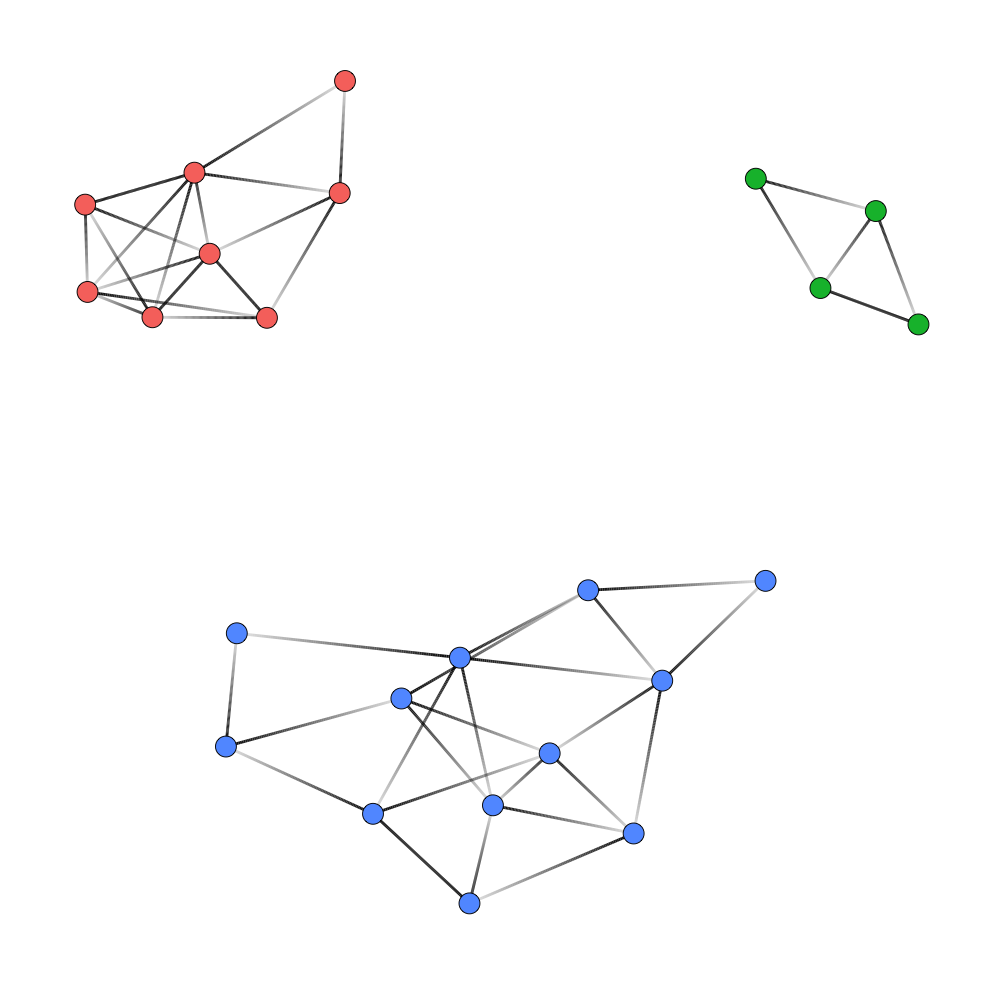
\includegraphics[width = 0.7\textwidth]{Images/struc_zero_nets.png}
% \caption[Directed network diagram generated from the example big network adjacency matrix]{Network diagram generated from the example combined network adjacency matrix depicted in Figure \ref{tab:combined}. None of the networks overlap.}
% \label{fig:struc_zero_nets}
% \end{figure}

\citet{gould1989structures} estimated the statistical significance of their five broker roles using a simple $p^1$ model. Their approach does not account for other possible network effects and tie dependencies that are likely to produce distorted results. Modifications were made to \texttt{MPNet} to allow the statistical significance of the different broker roles to be estimated more accurately. Parameter estimates based on a simple $p^1$ model were compared with those produced by the \texttt{sna} package \citep{butts2016sna} to check the modifications to \texttt{MPNet} were in agreement with \citet{gould1989structures}. The modified software was used in the second set of model estimations to characterise the three open innovation partnerships in terms of the mix of significant broker roles. Table \ref{tab:ergm_params} lists the model parameters used in this study. Appendix \ref{app:formulae} lists the statistical formulae for these parameters. \medskip

\begin{table}[!htbp]
\centering
\resizebox{\textwidth}{!}{%	
\begin{threeparttable}
\footnotesize
\setlength{\tabcolsep}{6pt}
\renewcommand{\arraystretch}{1}
\caption[Exponential random graph model parameters]{Exponential random graph model parameters used in this study*.}
\label{tab:ergm_params}
\begin{tabular}{lcl}
\toprule
\textbf{Parameter} & \textbf{Graphic} & \textbf{Explanation}  \\ \midrule
\textbf{Purely structural effects} & & \\
Arc (edge) & \begin{minipage}{.2\textwidth} \centering 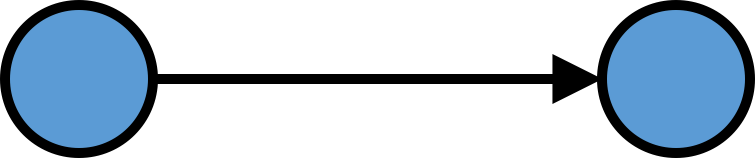
\includegraphics[width=0.4\linewidth]{Images/Arc} \end{minipage} & \begin{tabular}[c]{l}Baseline tendency for a tie to form\\ effects.\end{tabular} \\ \\
Reciprocity (mutuality)	& \begin{minipage}{.2\textwidth} \centering 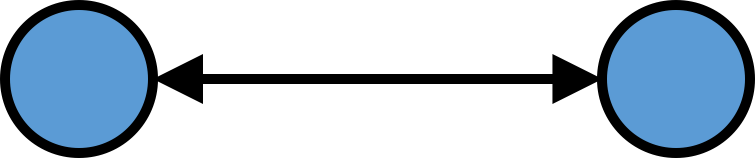
\includegraphics[width=0.4\linewidth]{Images/Reciprocity} \end{minipage} & \begin{tabular}[c]{l}Tendency for a tie from one actor to a second when there\\ is already a tie from the second to the first.\end{tabular} \\ \\ TwoPath (simple connectivity) & \begin{minipage}{.2\textwidth} \centering 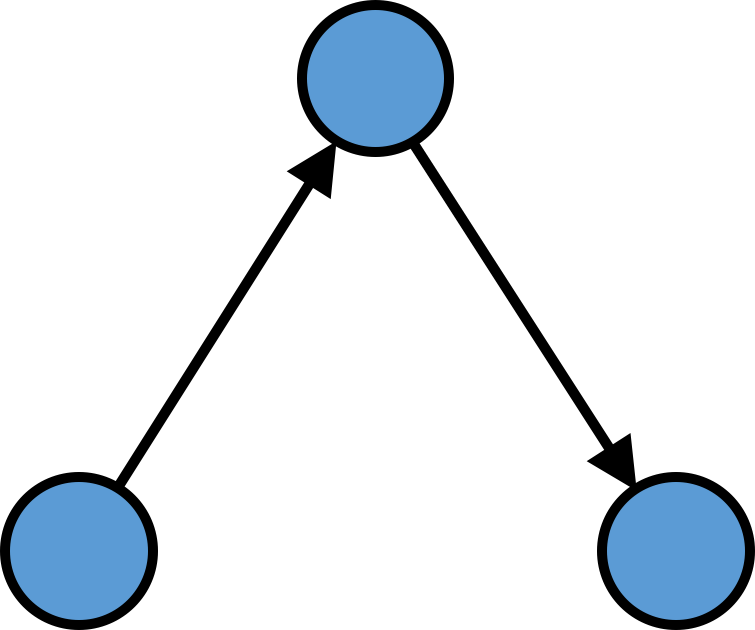
\includegraphics[width=0.4\linewidth]{Images/TwoPath} \end{minipage} & \begin{tabular}[c]{l}Tendency for ties to form as part of simple path formations. \end{tabular} \\ \\
AinS (popularity spread) & \begin{minipage}{.2\textwidth} \centering 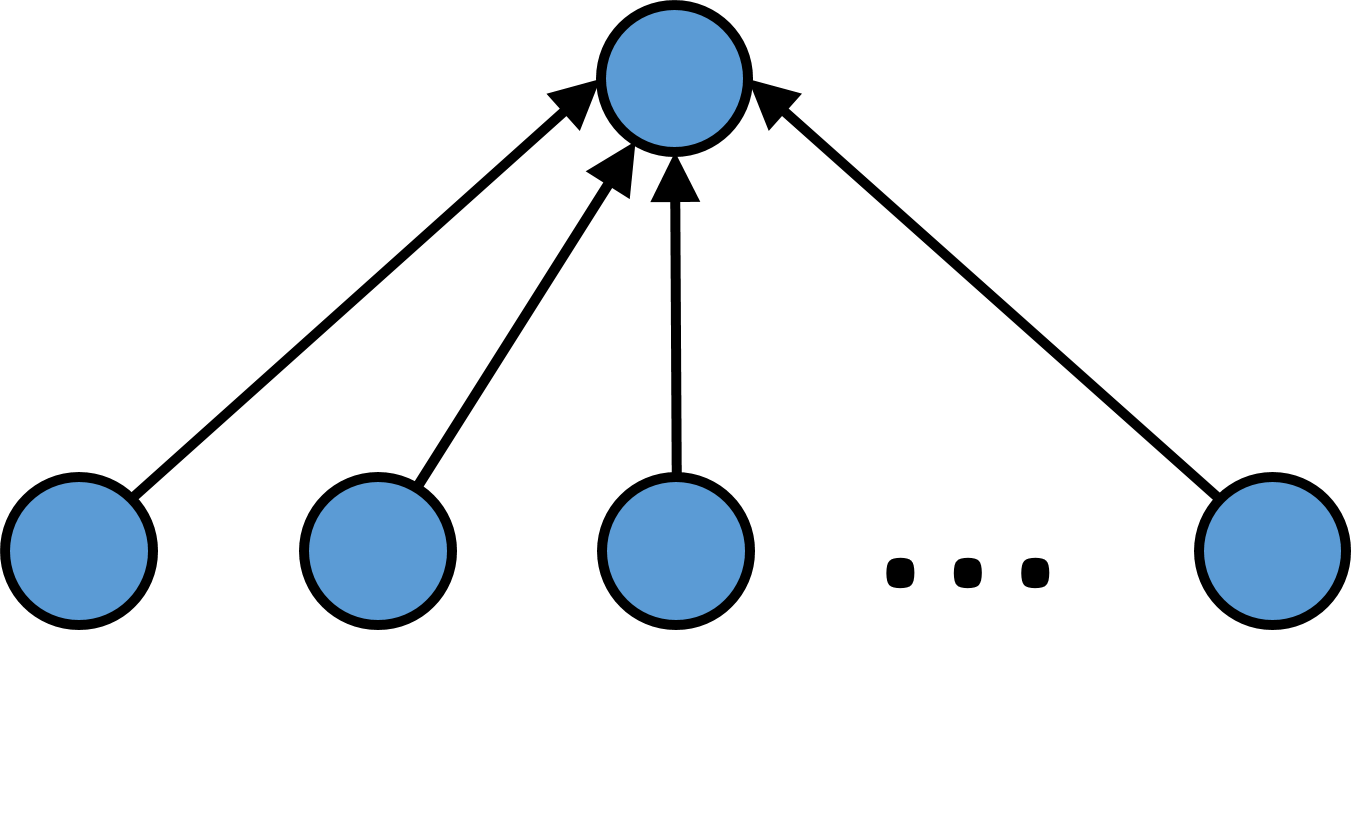
\includegraphics[width=0.6\linewidth]{Images/AinS} \end{minipage} & \begin{tabular}[c]{l}Propensity for dispersion in the in-degree distribution,\\ indicating there are a few highly popular actors. \end{tabular} \\ \\
AoutS (activity spread) & \begin{minipage}{.2\textwidth} \centering 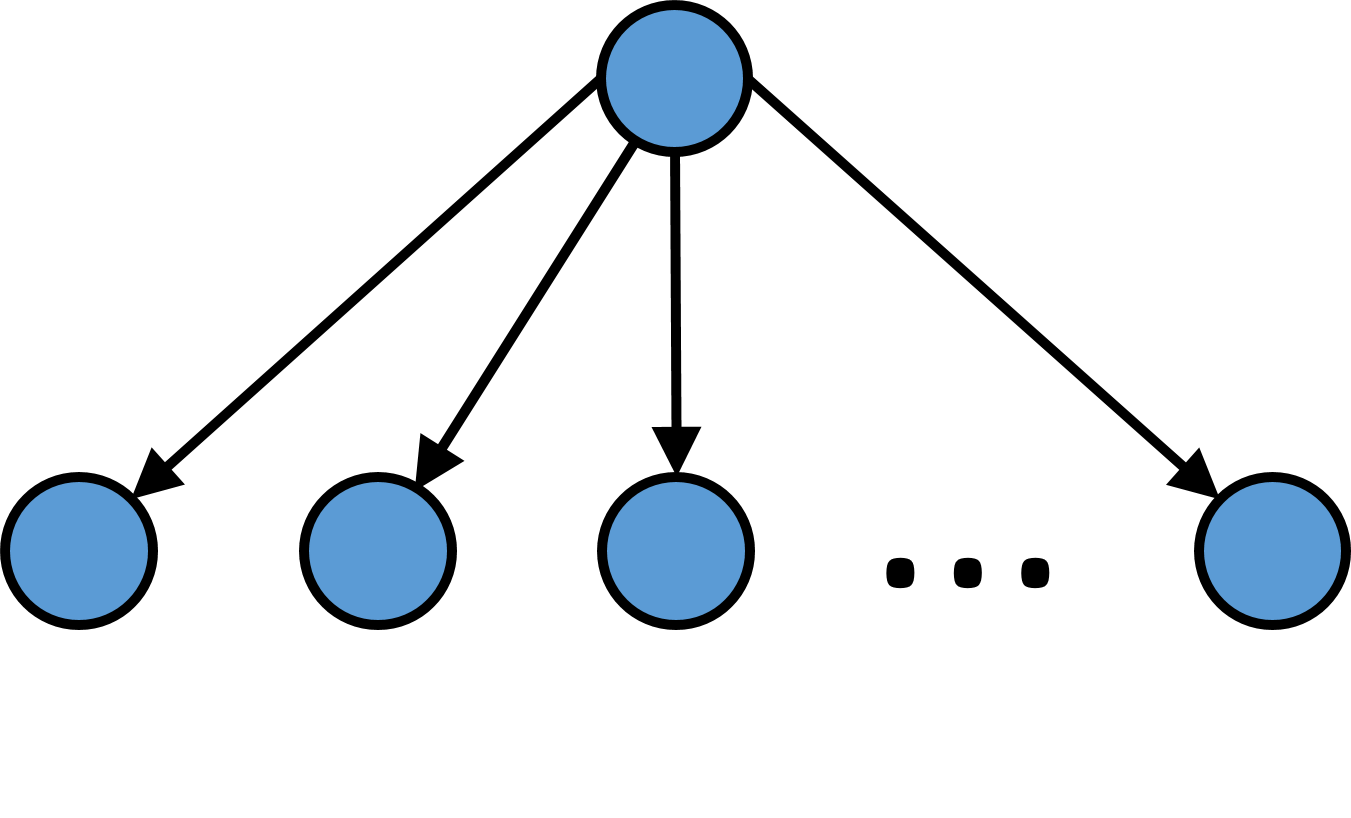
\includegraphics[width=0.6\linewidth]{Images/AoutS} \end{minipage} & \begin{tabular}[c]{l}Propensity for dispersion in the out-degree distribution,\\ indicating there are a few highly active actors. \end{tabular}  \\ \\
AT-T (path closure) & \begin{minipage}{.2\textwidth} \centering 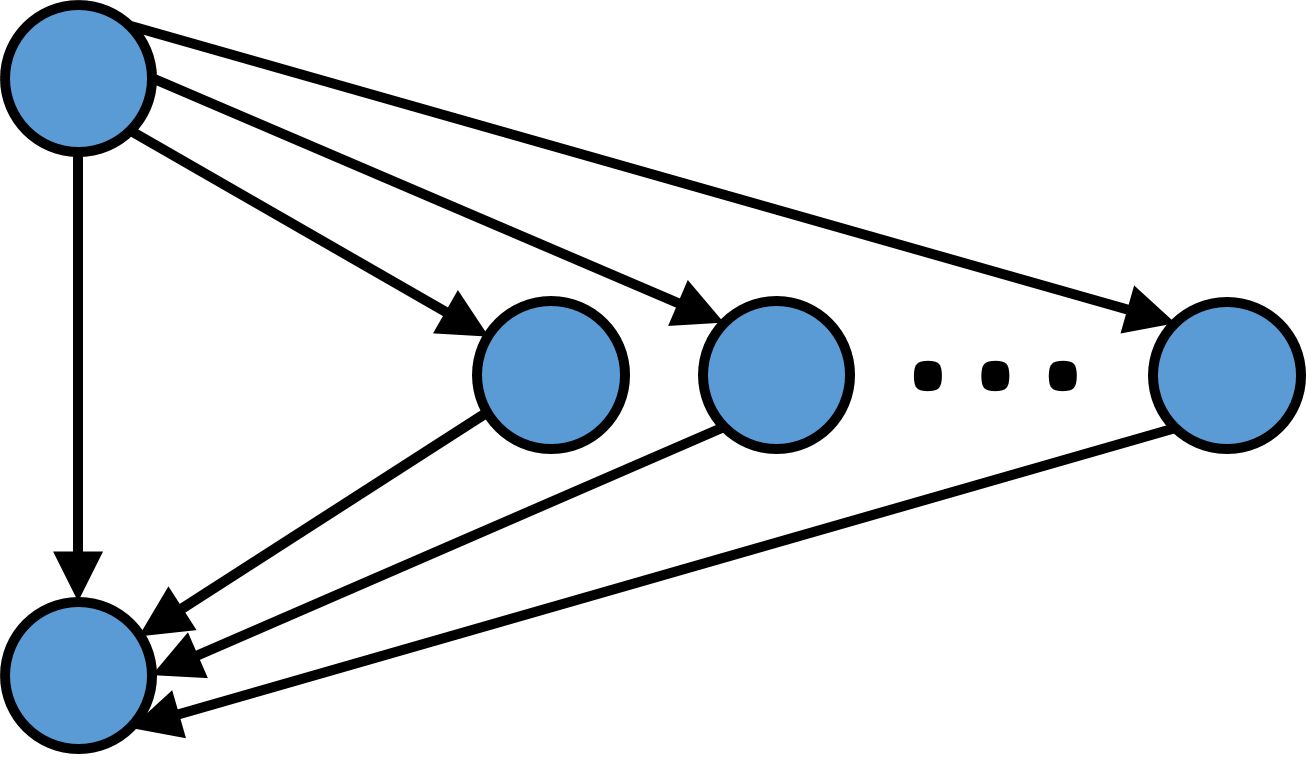
\includegraphics[width=0.6\linewidth]{Images/AT-T} \end{minipage} & \begin{tabular}[c]{l}Propensity for ties to form as part of transitive triad or a\\ multiple transitive configuration. \end{tabular} \\ \\
A2P (multiple connectivity) & \begin{minipage}{.2\textwidth} \centering 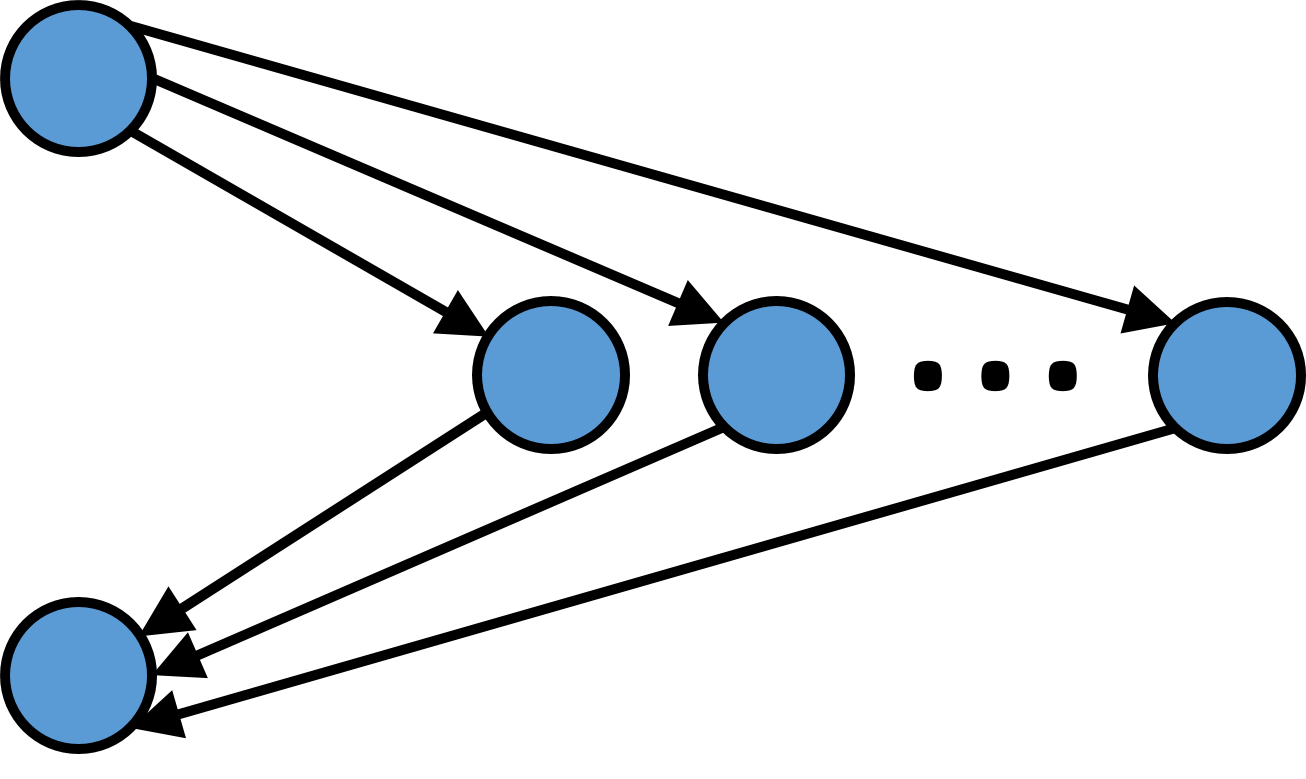
\includegraphics[width=0.6\linewidth]{Images/A2P} \end{minipage} & \begin{tabular}[c]{l}Propensity for ties to form as part of formations involving\\ multiple short paths between actors. \end{tabular} \\ \\
\textbf{Actor-relation effects} & & \\
Attribute sender & \begin{minipage}{.2\textwidth} \centering 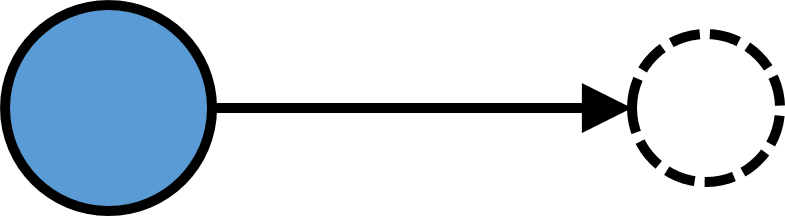
\includegraphics[width=0.4\linewidth]{Images/Sender} \end{minipage}	& \begin{tabular}[c]{l}Propensity for a tie to be directed from an actor with a\\ particular attribute. \end{tabular} \\ \\
Attribute receiver & \begin{minipage}{.2\textwidth} \centering 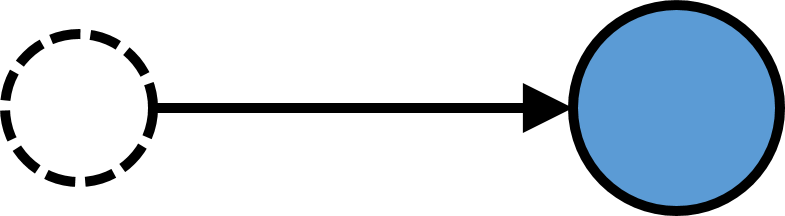
\includegraphics[width=0.4\linewidth]{Images/Receiver} \end{minipage} & \begin{tabular}[c]{l}Propensity for a tie to be directed toward an actor with a\\ particular attribute. \end{tabular} \\ \\
Attribute difference & \begin{minipage}{.2\textwidth} \centering 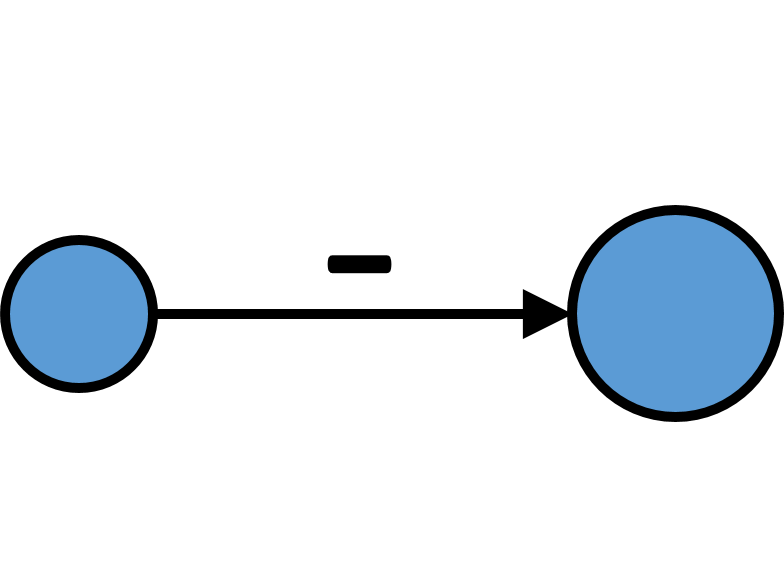
\includegraphics[width=0.4\linewidth]{Images/Difference} \end{minipage} & \begin{tabular}[c]{l}Propensity for a tie to form between actors with a similar\\ continuous attribute. \end{tabular} \\ \\
Attribute match & \begin{minipage}{.2\textwidth} \centering 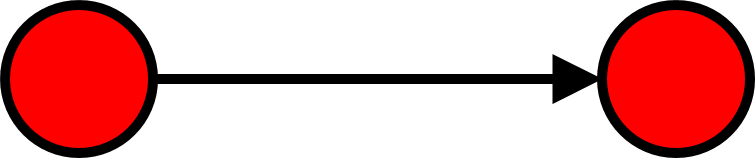
\includegraphics[width=0.4\linewidth]{Images/Match} \end{minipage} & \begin{tabular}[c]{l}Propensity for a tie to form between actors with the same\\ categorical attribute.\end{tabular} \\ \\
Attribute mismatch reciprocity & \begin{minipage}{.2\textwidth} \centering 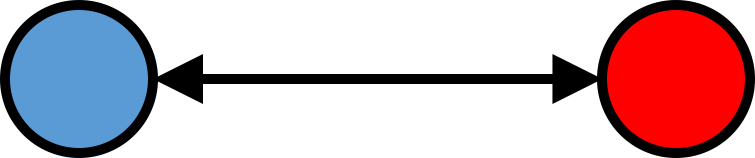
\includegraphics[width=0.4\linewidth]{Images/MisMatchReciprocity} \end{minipage} & \begin{tabular}[c]{l}Propensity for a tie to form between actors with a\\ non-matching categorical attribute.\end{tabular} \\ \\
b\textsubscript{O} (liaison role) & \begin{minipage}{.2\textwidth} \centering 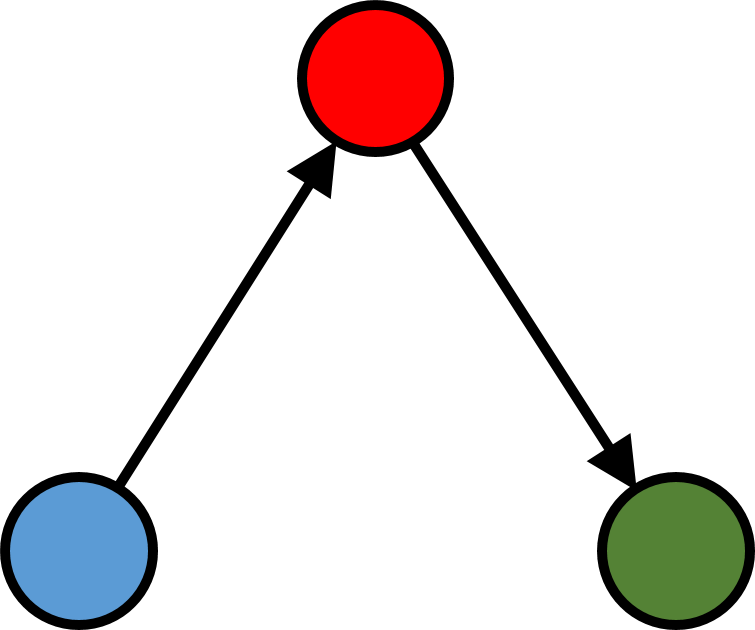
\includegraphics[width=0.4\linewidth]{Images/b_O} \end{minipage} & \begin{tabular}[c]{l}Propensity to have brokers who mediate communication\\ between two individuals from different groups, neither of\\ which they belong to.\end{tabular}\\ \\
b\textsubscript{IO} (representative role) & \begin{minipage}{.2\textwidth} \centering 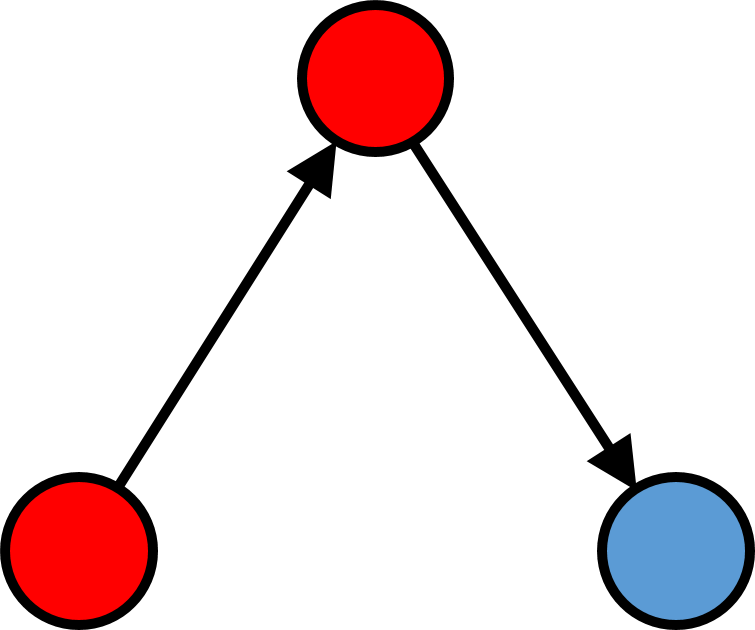
\includegraphics[width=0.4\linewidth]{Images/b_IO} \end{minipage} & \begin{tabular}[c]{l}Propensity to have brokers who mediate communication\\ from in-group members to out-group members. \end{tabular}\\ \\
b\textsubscript{OI} (gatekeeper role) & \begin{minipage}{.2\textwidth} \centering 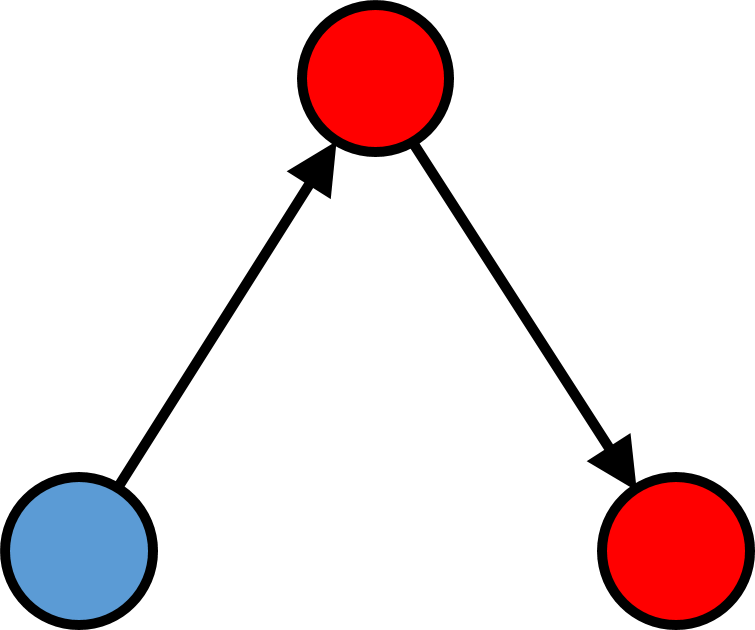
\includegraphics[width=0.4\linewidth]{Images/b_OI} \end{minipage} & \begin{tabular}[c]{l}Propensity to have brokers who mediate communication\\ from out-group members to in-group members. \end{tabular}\\ \\
w\textsubscript{O} (itinerant broker) & \begin{minipage}{.2\textwidth} \centering 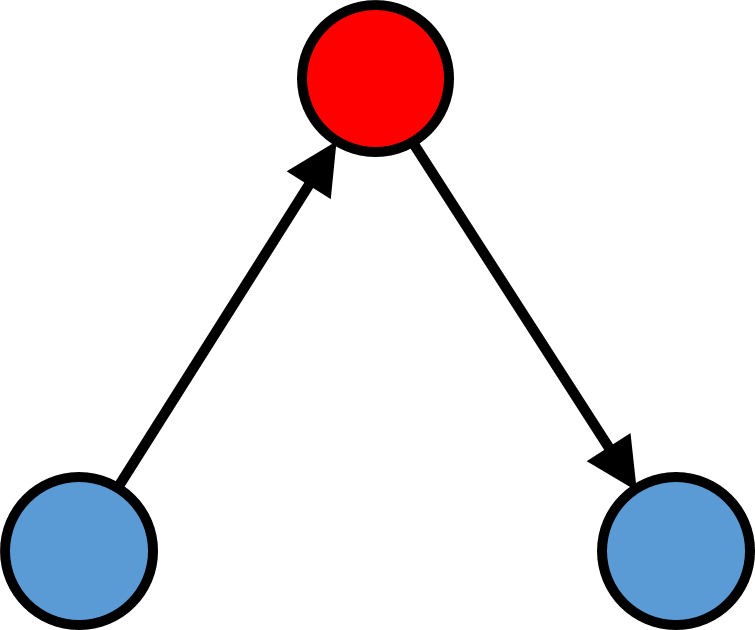
\includegraphics[width=0.4\linewidth]{Images/w_O} \end{minipage} & \begin{tabular}[c]{l}Propensity to have brokers who mediate communication\\ between two individuals from a single group to which they\\ do not belong. \end{tabular}\\ 
w\textsubscript{I} (coordination role) & \begin{minipage}{.2\textwidth} \centering 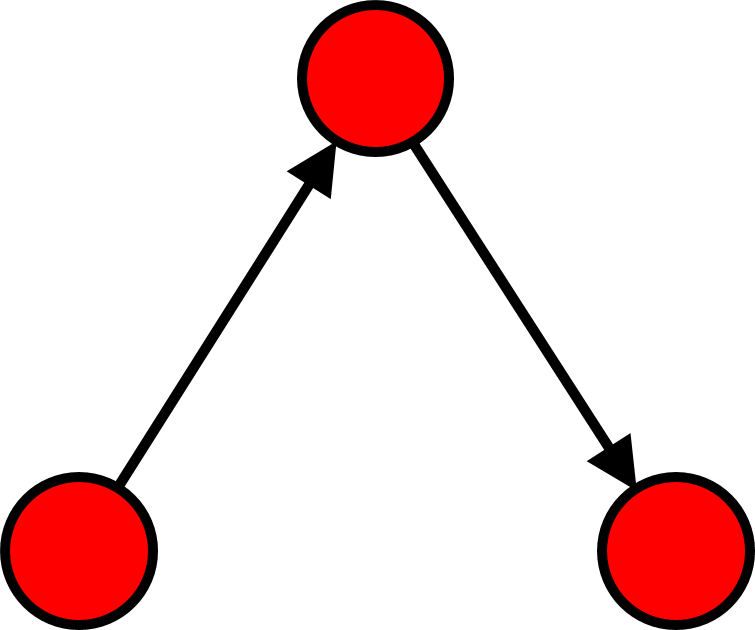
\includegraphics[width=0.4\linewidth]{Images/w_I} \end{minipage} & \begin{tabular}[c]{l}Propensity to have brokers who mediate communication\\ between two individuals from his or her own group. \end{tabular}\\ \\	
\textbf{Network covariate effects} & & \\
Dyadic covariate & \begin{minipage}{.2\textwidth} \centering 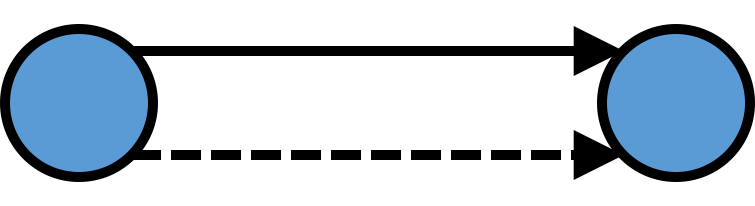
\includegraphics[width=0.4\linewidth]{Images/DyadicCovariate} \end{minipage} & \begin{tabular}[c]{l}Propensity for a tie of one type to form from one actor to\\ another if a tie of another type is already present, though\\ the covariate network is fixed (i.e. exogenous) in the\\ model, and so cannot vary. \end{tabular} \\\bottomrule
\end{tabular}

\begin{tablenotes}
\footnotesize
\item[*] Refer to Appendix \ref{app:formulae} for each parameter's network statistic.
\end{tablenotes}
\end{threeparttable}
}%
\end{table}

\section{Qualitative procedures}

\subsection{Data collection}

Follow-up interviews with a subset of survey participants make up the qualitative component of this study. Results from the exploratory data analysis of survey data were used to identify potential interviewees. Two criteria were used to identify which participants to interview, namely their network position and availability or willingness to be interviewed. Network position refers to the centrality of actors in the [tacit + explicit] knowledge provider network. The aim was to identify central and peripheral actors in the network, i.e. both powerful and less powerful actors. Some of the more central participants were unavailable to be interviewed because of pressing work commitments. Others were not comfortable being interviewed in English. The interviews covered 33\% of Case 1 participants, 32\% of Case 2 participants, and 17.5\% of Case 3 participants. Most of the participants interviewed reside in Australia. Of the 21 interviews conducted, 13 were face-to-face, and the rest were done via video-link. Two participants who live abroad were interviewed face-to-face while visiting Australia. \medskip

\subsubsection{Semi-structured interview questions}

The semi-structured interview questions were designed to explore the following constructs identified from the network data and relevant literature: industry context, partner history, the chronology of key events, the strength of the partnership, organisational culture, power relations, attitudes towards knowledge sharing and innovation, levels of motivation and trust, governance structures, and organisational learning capacity. Refer to Table \ref{tab:interview} in Appendix C for the list of questions used in the interviews. Interviews were designed to be completed in under an hour. The administration of semi-structured interviews was subject to ethics approval. 

\subsubsection{Interview protocol}

All the interviews were done by the author, either face-to-face or via video conference (using Skype\texttrademark). Each interview was recorded (using a digital memo recorder in the case of face-to-face interviews and a third-party plug-in recorder for Skype\texttrademark\ interviews). At the beginning of each interview, participants were asked to sign a consent form, permitting the use of the interview transcript in this study. Only then could recording start. \medskip

The number of questions asked in each interview varied according to the individual circumstances. Each interviewee was asked to comment on network diagrams depicting knowledge sharing, idea generation, and trust relations in their specific open innovation partnership. Showing network diagrams helped maintain a strong focus on partner behaviour and to solicit useful contextual information. \medskip

After each interview, interviewees were thanked and told they would receive a copy of the transcribed interview via email. They could withdraw their consent for the use of transcribed data if they felt uncomfortable with the contents thereof. 

\subsection{Data processing}

\subsubsection{Transcription of audio recordings}

The audio recordings of each interview were saved as MP3 files. Unfortunately, one Skype\texttrademark\ interview could not be transcribed as it failed to record correctly. The audio quality of another Skype\texttrademark\ recording was too poor for accurate transcription. Usable audio files were uploaded to a third-party transcription service (\url{http://www.transcriberonline.com/}). This service used manual transcribing that yielded very accurate transcriptions. The turnaround time for completing audio transcriptions was around three days. Transcriptions were provided as Microsoft Word\texttrademark\ documents. Each interviewee was allowed to comment on their interview transcription before qualitative analysis. None of the interviewees reported any issues. 

\subsubsection{Qualitative data analysis software}

Transcriptions were analysed using NVivo\texttrademark, a qualitative data analysis software (QDAS) package. This package facilitates manual coding of qualitative data and subsequent organisation and analysis of coded data \citep{bazeley2013qualitative}. NVivo\texttrademark\ allows one to work directly with the text, selecting passages, and doing coding onscreen. The same passage of text can have multiple codes. It is easy to insert annotations, comments, or analytic memos related to a specific code. Not only is it possible to immediately review coded text, one can easily combine, assemble, and re-arrange codes into new categories or themes in the process of \enquote{coding\hyp{}on} \citep{richards2012readme}. NVivo\texttrademark\ supports complex data queries, offers different ways to visualise coded data, and provides various analytical reports \citep{bazeley2013qualitative}. 

\subsubsection{Critical realist analytical framework} \label{sss:cr_framewk}

A code in qualitative data analysis is usually a word or short phrase that captures a meaningful attribute for a portion of text-based or visual data \citep{saldana2015coding}. There are many ways to code, but all share a common goal, namely extracting meaning from messy and unstructured qualitative data \citep{richards2012readme}. The process of coding involves assigning labels to individual words or chunks of text, sorting labels into different categories, grouping categories into broad themes, and then figuring out what these themes reveal about a given context. \medskip

Unfortunately, the literature on how to code qualitative data from a critical realist perspective is quite scant \citep{fletcher2017applying}. A key objective in critical realism is to look for patterns in empirical data that contribute to the generation of broad propositions or specific hypotheses about causal mechanisms \citep{zachariadis2013methodological}. This study uses a critical realist analytical framework developed by \cite{bygstad2016identifying} and further refined by \citet{mcavoy2018critical}. Figure \ref{fig:cr_steps} outlines the three main steps of this analytical framework. \medskip
 
\begin{figure}[hbt!]
\centering
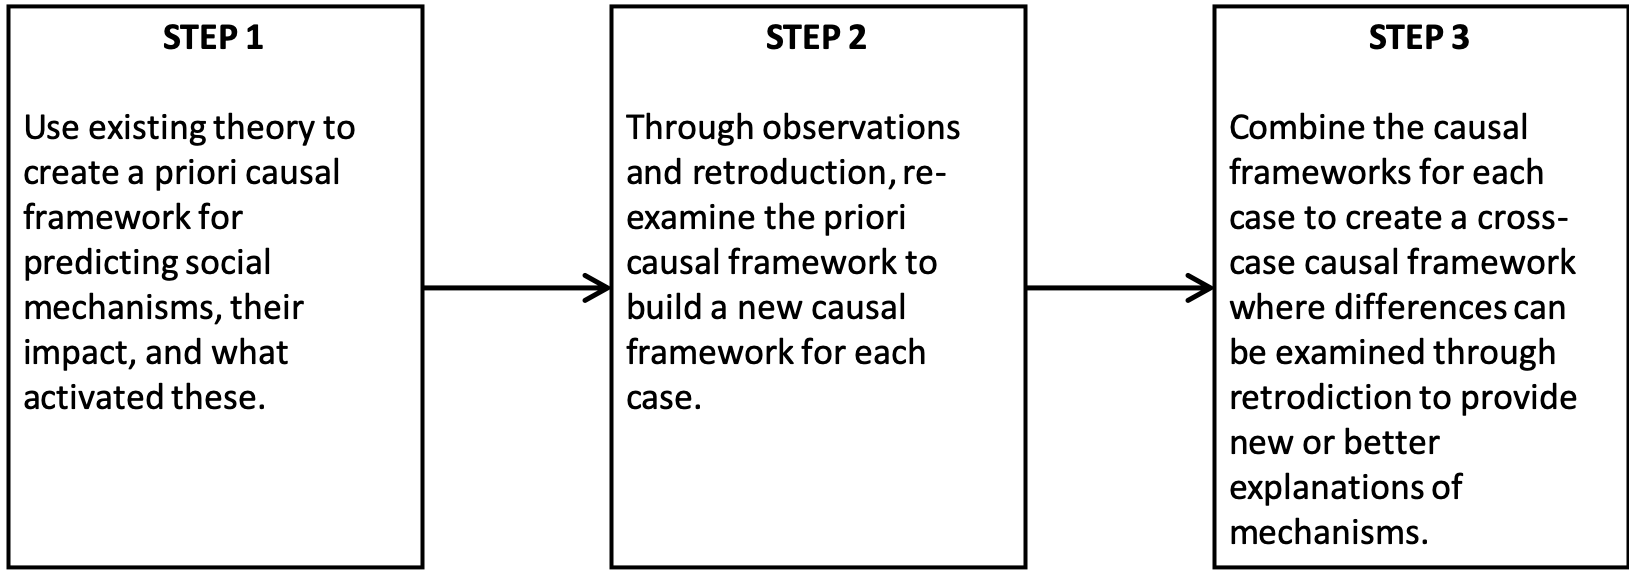
\includegraphics[width = 0.9\textwidth,
height = 0.7\textheight, keepaspectratio]{Images/cr_steps.png}
\caption[Critical realist analytical process]{Critical realist analytical process (after \cite{mcavoy2018critical})}
\label{fig:cr_steps}
\end{figure}

This study argues that agency lies at the heart of tacit knowledge sharing. It embraces \citeauthor{parsons1937structure}'s \citeyearpar{parsons1937structure} idea that individuals act to satisfy innate needs and that existing conditions and available means moderate their actions \citep{loyal2001agency}. The first step of our critical realist approach assumes that individuals choose to share or seek out tacit knowledge to satisfy an innate need for self-determination and adhere to subjective norms. Tempering the decision to share or seek tacit knowledge are external factors such as the presence of boundaries (e.g. organisational, disciplinary, or cultural boundaries), rules of engagement (e.g. contractual arrangements, appropriability regimes), trust (i.e. interpersonal and inter-organisational trust), and power relations (e.g.power-over versus power-to). We argue that skilled brokerage plays a crucial role in helping individuals overcome boundaries, build trust, and manage power relations. Figure \ref{fig:agency_structure2} represents the prior causal framework based on \citeauthor{loyal2001agency}'s \citeyearpar{loyal2001agency} refinement of \citeauthor{parsons1937structure}'s \citeyearpar{parsons1937structure} idea. We use the theories of self-determination \citep{ryan2000self}, planned behaviour \citep{ajzen1985intentions}, social exchange \citep{blau1964exchange}, power relations \citep{emerson1962power}, and brokerage \citep{marsden1982brokerage,burt2005brokerage,obstfeld2014brokerage} to elaborate the framework through a set of propositions, which serve as a starting point for our critical realist analysis (the first step of analysis). \medskip

\begin{figure}[hbt!]
    \centering
    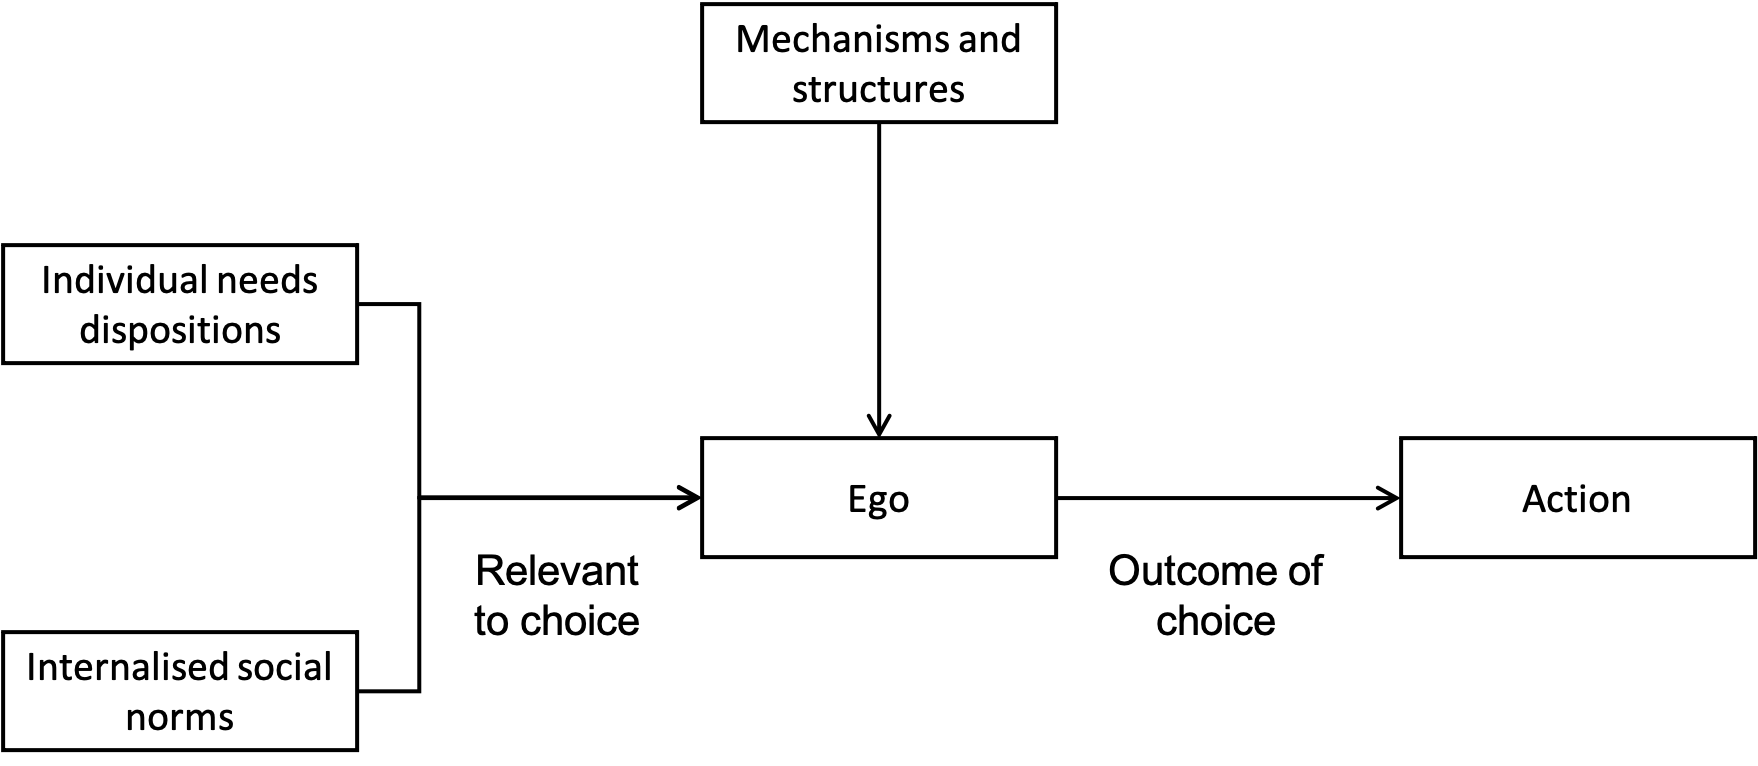
\includegraphics[width = \textwidth]{Images/agency_structure_loyal.png}
    \caption[]{Critical realist perspective of agency versus structure. Agency is about making intentional choices. Choices may be tempered by internalised social norms and social reality more broadly \citep{loyal2001agency}.}
    \label{fig:agency_structure2}
\end{figure}

The second step combines the results of the social network analysis with the coding of the semi-structured interviews. We derived a set of provisional codes from the theoretical propositions developed in Chapters 2 and 3. The provisional codes were expanded upon through inductive coding of interview transcripts. Expanded codes were then grouped into category codes. The category codes refer to the main elements of \citeauthor{loyal2001agency}'s \citeyearpar{loyal2001agency} agency mode (Figure \ref{fig:agency_structure2}). Coded segments of interview transcripts describe the initial constructs in context, draw attention to hidden constructs, and provide a foundation for inductively forming higher-level categories of codes \citep{saldana2015coding}. Efforts to discover unobserved mechanisms and interacting structures also help expose potential researcher bias with initial constructs. The codes were prioritised according to frequency of mention for the next stage of analysis. \medskip

In the final third and final step, we use the logic of retroduction to develop a causal framework for each case and then the logic of retrodiction to combine the causal frameworks for each case, allowing us to provide new or better explanations of tacit knowledge sharing mechanisms \citep{mcavoy2018critical}. This approach delivers an updated set of propositions that can account for what is happening in practice and what is driving practice. Figure \ref{fig:coding_process} summarises the critical realist coding process used in this study. Codes from each case were recorded into a universal codebook (a codebook is a compilation of all the codes, their content descriptions, and a brief data example for reference) \citep{guest2011applied}. 

\begin{sidewaysfigure}
\centering
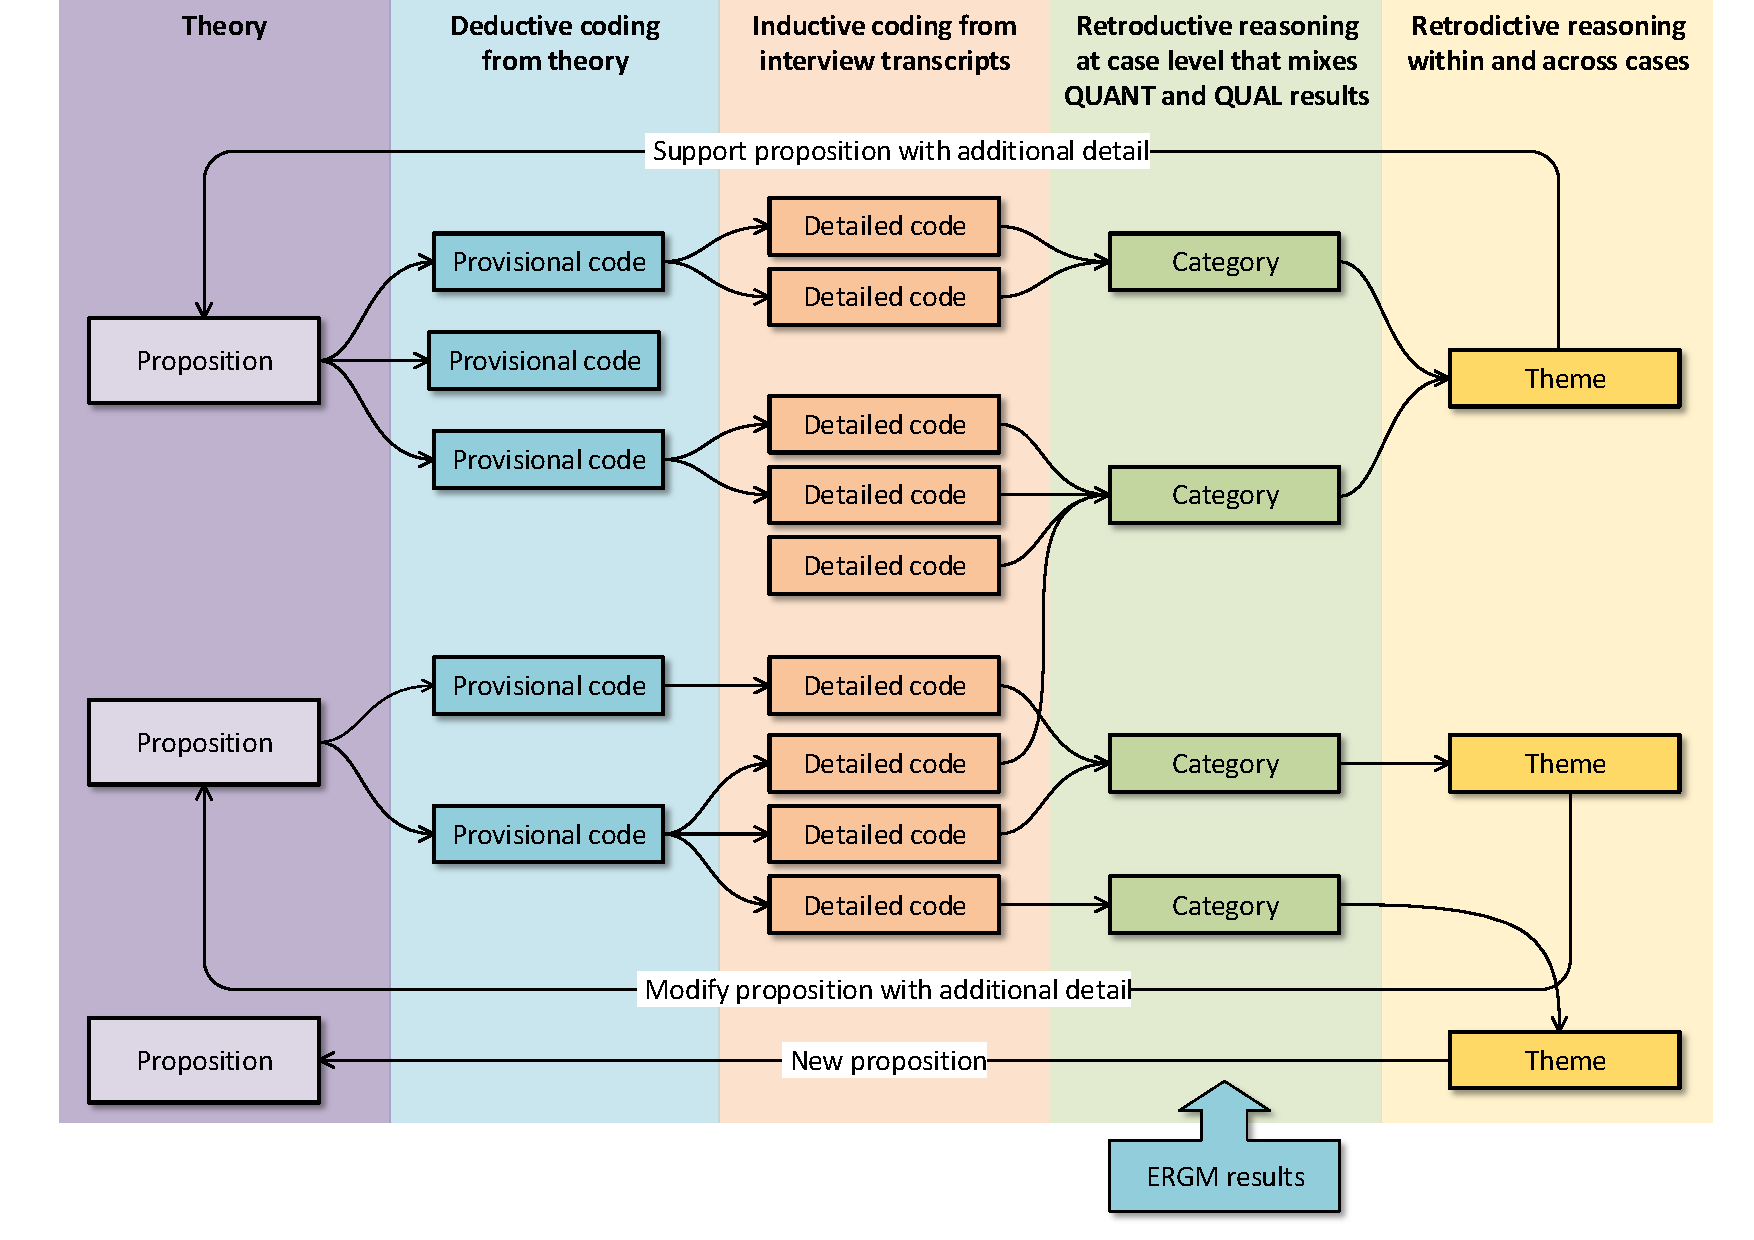
\includegraphics[width = 0.9\textwidth,
height = 0.7\textheight, keepaspectratio]{Images/CR.pdf}
\caption[Critical realist coding process]{Critical realist coding process.}
\label{fig:coding_process}
\end{sidewaysfigure}

\section{Summary}

This thesis employs a mixed-methods approach to examine the social mechanisms that shape tacit knowledge sharing in three open innovation partnerships. An online survey was used to gather data about individual participants in each partnership and their social relations with fellow participants. Survey data were analysed using a combination of descriptive and statistical social network analysis techniques. The descriptive analysis measured actor centrality and two-path brokerage whereas the statistical analysis used ERGMs to assess the relative abundance or absence of specific network configurations. Semi-structured interviews involving a subset of the survey participants complemented the social network analysis. Mixing quantitative network and qualitative interview data can be fraught due to the complex ontological and epistemological issues involved. For this reason, a critical realist perspective was used to interpret quantitative and qualitative results. This thesis breaks new ground in applying a critical realist approach to mixed-method social network analysis. \medskip

The next chapter (Chapter \ref{chp:case_overview}) details the innovation challenge in each of the three open innovation cases recruited. Each case is quite different looking at their industrial context, the stage they are at, participant numbers, their demographic features, spatial proximity to one another, and patterns of social interaction. 

\chapter{Methodology}
\section{Introduction}

Recapping, this thesis characterises an open innovation partnership as a temporary knowledge network. We can use social network analysis to evaluate knowledge sharing practices in open innovation partnerships. The last chapter argued human agency lies at the heart of tacit knowledge sharing and suggested autonomous motivation, the disposition to trust, and power-relations in various social contexts influence an individual's decision to share or seek out tacit knowledge. Table \ref{tab:propos} lists the seven propositions developed in Chapters 2 and 3 and how these relate to the four research questions stated in Chapter 1. The propositions serve as an analytical framework for mixed-method inquiry, not as testable hypotheses. \medskip

This chapter explains the methodology used to assess the propositions across three open innovation partnerships. It includes justifications for embracing a critical realist worldview and employing a case-based mixed-method research design. The chapter details the quantitative and qualitative procedures used to collect and analyse data and the critical realist process used to interpret the data. 

\begin{sidewaystable}[p]
\centering
\caption[Research questions and related propositions]{Research questions and related propositions.}
\label{tab:propos}
\renewcommand{\arraystretch}{1.2}
\resizebox{0.9\textwidth}{!}{%	
\begin{tabular}{lcl}
\toprule
 \multicolumn{1}{c}{Research question} &&  \multicolumn{1}{c}{Related proposition(s)} \\ \midrule
 
\begin{minipage}{0.35\linewidth}\renewcommand{\theenumi}{\arabic{enumi}} \begin{enumerate} \setcounter{enumi}{0} \item What does the structure of tacit knowledge networks reveal about knowledge enacted in practice? \end{enumerate}\end{minipage} && \begin{minipage}{0.55\linewidth} \renewcommand{\theenumi}{\alph{enumi}} \begin{enumerate}
    \item Open innovation is about connecting practitioners across organisational and disciplinary boundaries so that they can apply their know-how in novel ways.
    \item Relative differences in absorptive capacity limit the potential value of inter-organisational knowledge networks. Reducing the cognitive distance between open innovation partners requires significant social interaction to support learning and the application of knowledge in practice.
\end{enumerate} \end{minipage} \\ \midrule
 
\begin{minipage}{0.35\linewidth}\renewcommand{\theenumi}{\arabic{enumi}} \begin{enumerate} \setcounter{enumi}{1} \item Does brokerage differ according to the type of knowledge being exchanged? \end{enumerate}\end{minipage} && \begin{minipage}{0.55\linewidth} \renewcommand{\theenumi}{\alph{enumi}} \begin{enumerate} \item Successful open innovation requires a combination of skilled brokerage and network closure. \end{enumerate} \end{minipage} \\ \midrule

\begin{minipage}{0.35\linewidth}\renewcommand{\theenumi}{\arabic{enumi}} \begin{enumerate} \setcounter{enumi}{2} \item To what extent does self-determination drive tacit knowledge sharing in open innovation? \end{enumerate} \end{minipage} && \begin{minipage}{0.55\linewidth}\renewcommand{\theenumi}{\alph{enumi}}\begin{enumerate}
\item Since agency lies at the heart of tacit knowledge sharing, too much formal structure will inhibit tacit knowledge exchange in open innovation partnerships. 
\item Significant effort is required to socialise tacit knowledge. Subjective norms and other external forces may moderate individual willingness to seek out or share tacit knowledge. \end{enumerate} \end{minipage} \\ \midrule

\begin{minipage}{0.35\linewidth} \renewcommand{\theenumi}{\arabic{enumi}} \begin{enumerate} \setcounter{enumi}{3} \item What does the micro-structure of tacit knowledge networks reveal about trust and power-relations in open innovation partnerships? \end{enumerate} \end{minipage} && \begin{minipage}{0.55\linewidth}\renewcommand{\theenumi}{\alph{enumi}}\begin{enumerate}
\item People are more likely to exchange tacit knowledge with others they trust. Reciprocity and closure in tacit knowledge exchange networks indicate high levels of trust in open innovation partnerships. It is an indicator of swift trust when observed in relatively new partnerships. 
\item People share their tacit knowledge to empower themselves and others. Whom they choose to share their tacit knowledge with depends on how much they trust the receiver to use their knowledge in mutually beneficial ways. \end{enumerate} \end{minipage}\\ \bottomrule
\end{tabular}
}
\end{sidewaystable}

\section{Research design}

\subsection{Research paradigm}

A research paradigm describes a worldview informed by philosophical assumptions about the nature of reality (ontology - what do we believe about the nature of reality?), ways of knowing (epistemology - how do we know what we know?), and ethics and value systems (axiology - what do we believe is true?). We may treat ontology in terms of one verifiable reality or as multiple socially-constructed realities \citep{chilisa2012selecting}. Epistemology considers the nature of knowledge (versus the nature of reality) and involves asking questions about the sources of knowledge, the reliability of these sources, to what extent can we know about something, and how one can know if knowledge is real or not \citep{patton2002qualitative}. Methodology is where assumptions about the nature of reality, nature of knowledge, values, theory, and practice on a given topic come together \citep{chilisa2012selecting}. 

\subsubsection{Positivist worldview}

Researchers studying the physical world tend to embrace a positivist paradigm, one that consists of a single tangible reality independent of cognition \citep{van2007engaged}. Positivists consider the scientific method as the only way to verify the existence of an objective reality \citep{creswell2011designing}. They see themselves as detached observers, able to reduce a problem into measurable parts, and demonstrate causality through statistical and mathematical methods \citep{easterby2015management}. Some argue that no matter how faithfully a researcher adheres to the scientific method, research outcomes are neither totally objective nor unquestionably absolute \citep[][p. 40]{crotty1998foundations}. The post-positivist paradigm accounts for bias and uncertainty by establishing causality through deductive falsification, unlike positivism which relies on inductive verification to generalise facts \citep{van2007engaged,chilisa2012selecting}. Efforts to ground social science in empirical investigations has led it to embrace a strongly positivist paradigm. By focusing more on epistemology than on ontology, social science has focused too much on methods and forms of explanation. Insufficient attention has been given to questions about what kind of entities actually exist in the social world and what are they like \citep{archer2016what}. 

\subsubsection{Constructivist worldview}

The constructivist paradigm assumes that reality is what people perceive it to be. Knowledge is considered to be subjective because it is socially constructed and dependent on personal beliefs and values \citep{chilisa2012selecting}. Since meaning is considered to exist within the human experience, the goal of constructivist research is to understand individual experiences. There is no preferred epistemology since discourses vary and are often incommensurable, and the research methodology reflects the assumptions of the researcher in attempting to interpret human experiences \citep{van2007engaged}. 

\subsubsection{Critical realist worldview}

In critical realism, reality is stratified into three ontological levels (see Figure \ref{fig:stratified_reality}). The first is the \textit{empirical} level, which refers to aspects of reality observed or experienced directly or indirectly otherwise described as the transitive level of reality where events occur \citep{fletcher2017applying}. The second level consists of the \textit{actual}, which refers to aspects of reality that may exist but are not necessarily observed or experienced \citep{mcevoy2006critical}. Events happen regardless of whether we experience or interpret them. Finally, the third level is the \textit{real} and refers to the structures and mechanisms that cause or influence events \citep{zachariadis2013methodological}. These structures and mechanisms are beyond the realm of human observation and experience. They cannot be known or perceived and must be inferred through deductive (empirical investigation) and inductive (theory construction) processes \citep{mcevoy2006critical,wynn2012principles}. \medskip

\begin{figure}
\centering
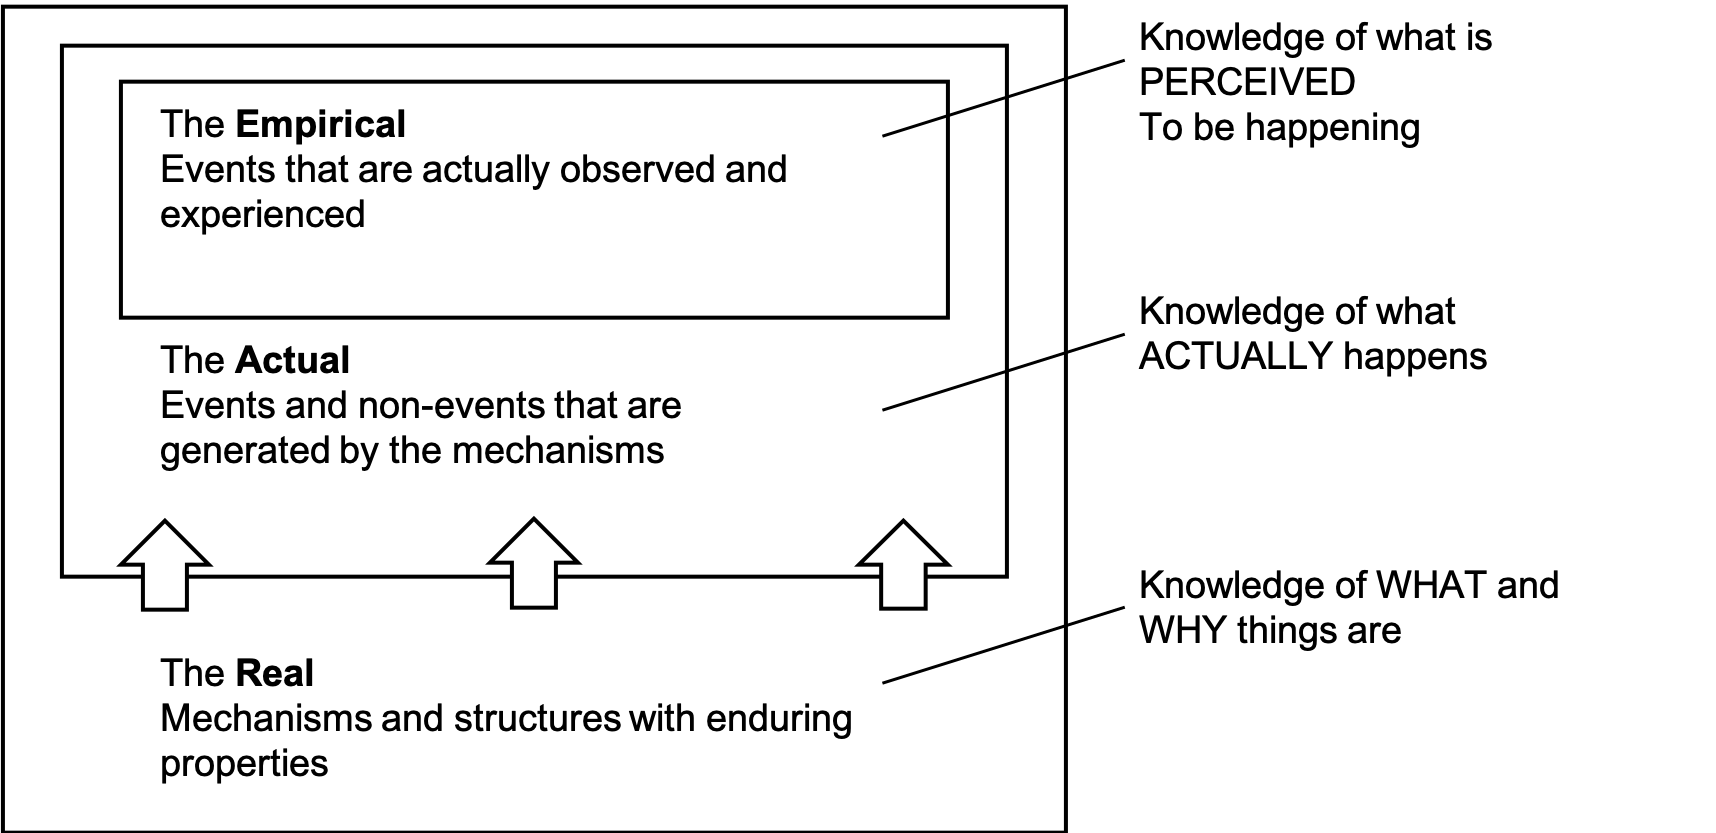
\includegraphics[width=0.9\linewidth]{Images/stratified_reality.png}
\caption[The stratified ontology of critical realism]{The stratified ontology of critical realism \citep{bhaskar2013realist,mingers2006realising}.}
\label{fig:stratified_reality}
\end{figure}

The critical realist applies the logic of retroduction to discover the interacting mechanisms and structures that may explain events \citep{sayer1999realism,wynn2012principles}. Retroduction suggests new ideas or explanations, some of which may, after testing by induction, turn out to be true (Figure \ref{fig:retroduction}). These mechanisms or structures can be physical, social, or psychological, and may not be directly observable except in terms of their effects (e.g. the configuration of network structures) \citep{mcavoy2018critical}. The primary goal of critical realism is to explain events through reference to these structures and mechanisms and the effects they can have across all three levels of reality \citep{wynn2012principles,fletcher2017applying}. \medskip

\begin{figure}[h!]
\centering
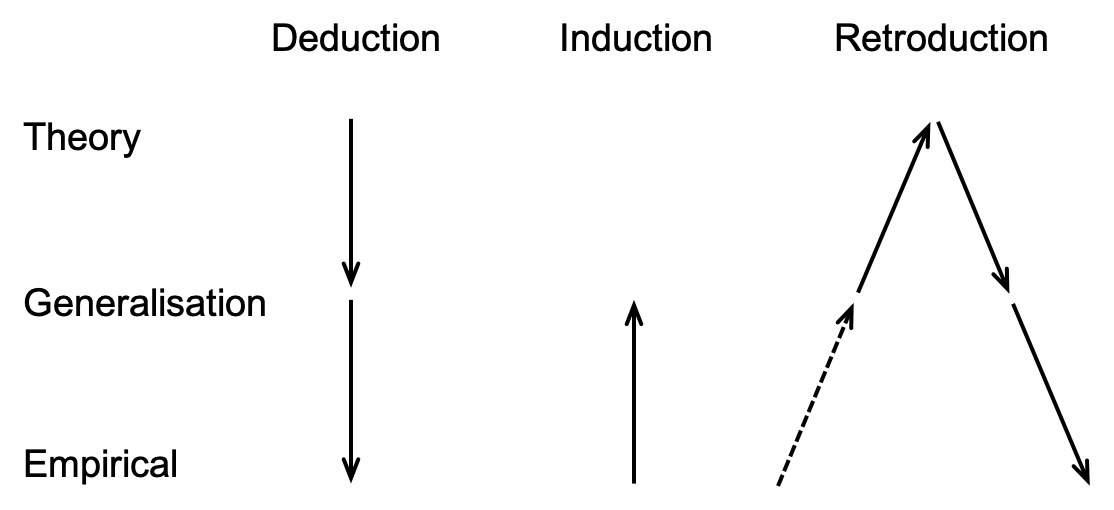
\includegraphics[width=0.7\linewidth]{Images/retroduction.png}
\caption[Logic of deduction, induction and retroduction]{Logic of deduction, induction and retroduction. Deduction is typically used to prove or disprove theory. Induction is used to generalise human experiences. Retroduction combines inductive and deductive reasoning to understand causal mechanisms as objectively as possible \citep{saether1998retroduction}.}
\label{fig:retroduction}
\end{figure}

\subsection{Justification for a critical realist approach}

This thesis aims to investigate mechanisms and structures that affect tacit knowledge sharing in open innovation. Though we can quantify social ties between participants and test hypotheses about tie formation in a positivist manner, this cannot account for external or experiential factors that influence tie formation. We need a combination of quantitative and qualitative methods to obtain a complete understanding of the mechanisms and structures affecting tacit knowledge sharing in open innovation. \medskip

Combining quantitative and qualitative methods is fraught because of the complex ontological and epistemological issues involved \citep{giddings2006mixed,mcevoy2006critical}. Methodological purists tend to be absolutist and argue strongly in favour of their preferred methodology. For them, quantitative and qualitative methods rely on mutually exclusive assumptions and are thus incommensurable \citep{greene2008mixed}. Methodological pragmatists, on the other hand, accept that assumptions can be mutually exclusive but assert that researchers should use whatever methods are needed to obtain useful results, even though this involves alternating between paradigms. The logic of methodological pragmatists is that neither quantitative nor qualitative methods alone are sufficient to develop a complete analysis \citep{mcevoy2006critical,creswell2013research}. Applying a pragmatic approach can be very challenging, especially when attempting to make sense of discordant data collected under different epistemological assumptions \citep{johnson2004mixed,giddings2006mixed}. Any study that involves mixing methods must reconcile ontological and epistemological differences to ensure findings are both credible and valid \citep{zachariadis2013methodological}. \medskip

The stratified ontology of critical realism allows for the \enquote{legitimate} combination of qualitative and quantitative methods. Table \ref{tab:mm_critical_realism} lists reasons for mixing methods in critical realism. In the case of this study, the quantitative analysis tested psychosocial theories to explain significant network effects. The quantitative analysis was \textit{complimented} by qualitative analysis of semi-structured interviews that allowed deeper exploration of the mechanisms and structures affecting tacit knowledge sharing in open innovation partnerships. Applying the logic of retroduction provided a more \textit{complete}, \textit{expansive} and \textit{diverse} picture of the mechanisms and structures affecting tacit knowledge sharing. \medskip

\begin{sidewaystable}[p]
\centering
\resizebox{0.9\textwidth}{!}{%	
\begin{threeparttable}
\footnotesize
\setlength{\tabcolsep}{6pt}
\renewcommand{\arraystretch}{1}
\caption[Reasons for mixing methods in critical realism]{Reasons for mixing methods in critical realism \citep{zachariadis2013methodological}.}
\label{tab:mm_critical_realism}
\begin{tabular}{p{4cm}p{8cm}p{8cm}}
\toprule
\multicolumn{1}{c}{\textbf{Goal}} & \multicolumn{1}{c}{\textbf{Description}} & \multicolumn{1}{c}{\textbf{Critical realist implication}} \\ \midrule
Complementarity & Mixed methods are used in order to gain complementary views about the same phenomena or events & Different levels of abstraction of a multi\hyp{}layered world demand different methods \\
Completeness & Mixed methods research design is used to ensure a complete picture (as detailed as possible) of the phenomenon under study & Requires meta-theoretical considerations \\
Developmental & Inferences of one type of research are being used as questions for another type of research & This being part of the retroductive approach of critical realism, inferences need to hypothesise about the causal mechanisms whose recovery will then inspire additional research \\
Expansion & Mixed methods are being implemented in order to provide explanations or expand the understanding obtained in previous research & Quantitative methods can be used to guide qualitative research which (subject to the context) is more capable of uncovering generative mechanisms \\
Confirmation & Mixed methods are used in order to confirm the findings from another study & Epistemic fallacy occurs when trying to validate qualitative results with quantitative methods \\
Compensation & The weakness of one method can be compensated by the use of another & The weaknesses of different methods are recognised so alternative methods can be used to compensate \\
Diversity & Mixed methods are used in order to obtain divergent views on the same phenomena & Different levels of abstraction of a multi- layered world demand different methods \\ \bottomrule
\end{tabular}\end{threeparttable}
%
}
\end{sidewaystable}

\subsection{Case-based research}

A case study involves detailed examination of a particular case or set of cases within a real-world context \citep{crowe2011case}. It is an established research design used extensively in a wide variety of disciplines. The case study approach lends itself well to capturing information on more explanatory \textquote{how}, \textquote{what} and \textquote{why} questions \citep{crowe2011case}. How one approaches a case study depends on one's epistemological standpoint. For example, \citet{eisenhardt1989building} argues that case studies are a good way to develop social theories. She advocates inductive theory-building research to highlight associations between constructs and variables that can be tested. Her approach seeks to establish regularities rather than the reasons behind them i.e. it emphasises generalisation over context \citep{welch2011theorising}. \citet{yin2009case}, on the other hand, prefers a more deductive approach to case studies. He thinks case studies are well-suited to test the validity of existing theories. His approach discounts contextual factors that may affect causal relationships \citep{welch2011theorising}. \citet{stake2005qualitative} argues that generalising the results of case studies is too simplistic and deterministic. He thinks the true value of case studies lies in understanding the uniqueness of each case. For him, it is all about understanding different contexts. \citet{welch2011theorising} argue that a critical realist approach offers a high degree of contextualisation without sacrificing the goal of causal explanation. Contextualised explanations can provide novel theoretical accounts that incorporate rather than deny complexity \citep{ragin2009reflections}. \medskip

\subsection{Mixed-methods research design}

This thesis uses a case-based mixed-method research design to unpack the social mechanisms and structures that shape tacit knowledge exchange ties in three open innovation partnerships. Figure \ref{fig:mm} outlines the different research stages of this study. The first step identified research gaps in the open innovation literature. These informed the research questions that are the focus of this study. The next step was to apply a critical realist research process to identify critical social mechanisms affecting tacit knowledge exchanges in open innovation partnerships, their impact, and how these are activated \citep{mcavoy2018critical}. \medskip

\begin{figure}[p]
\centering
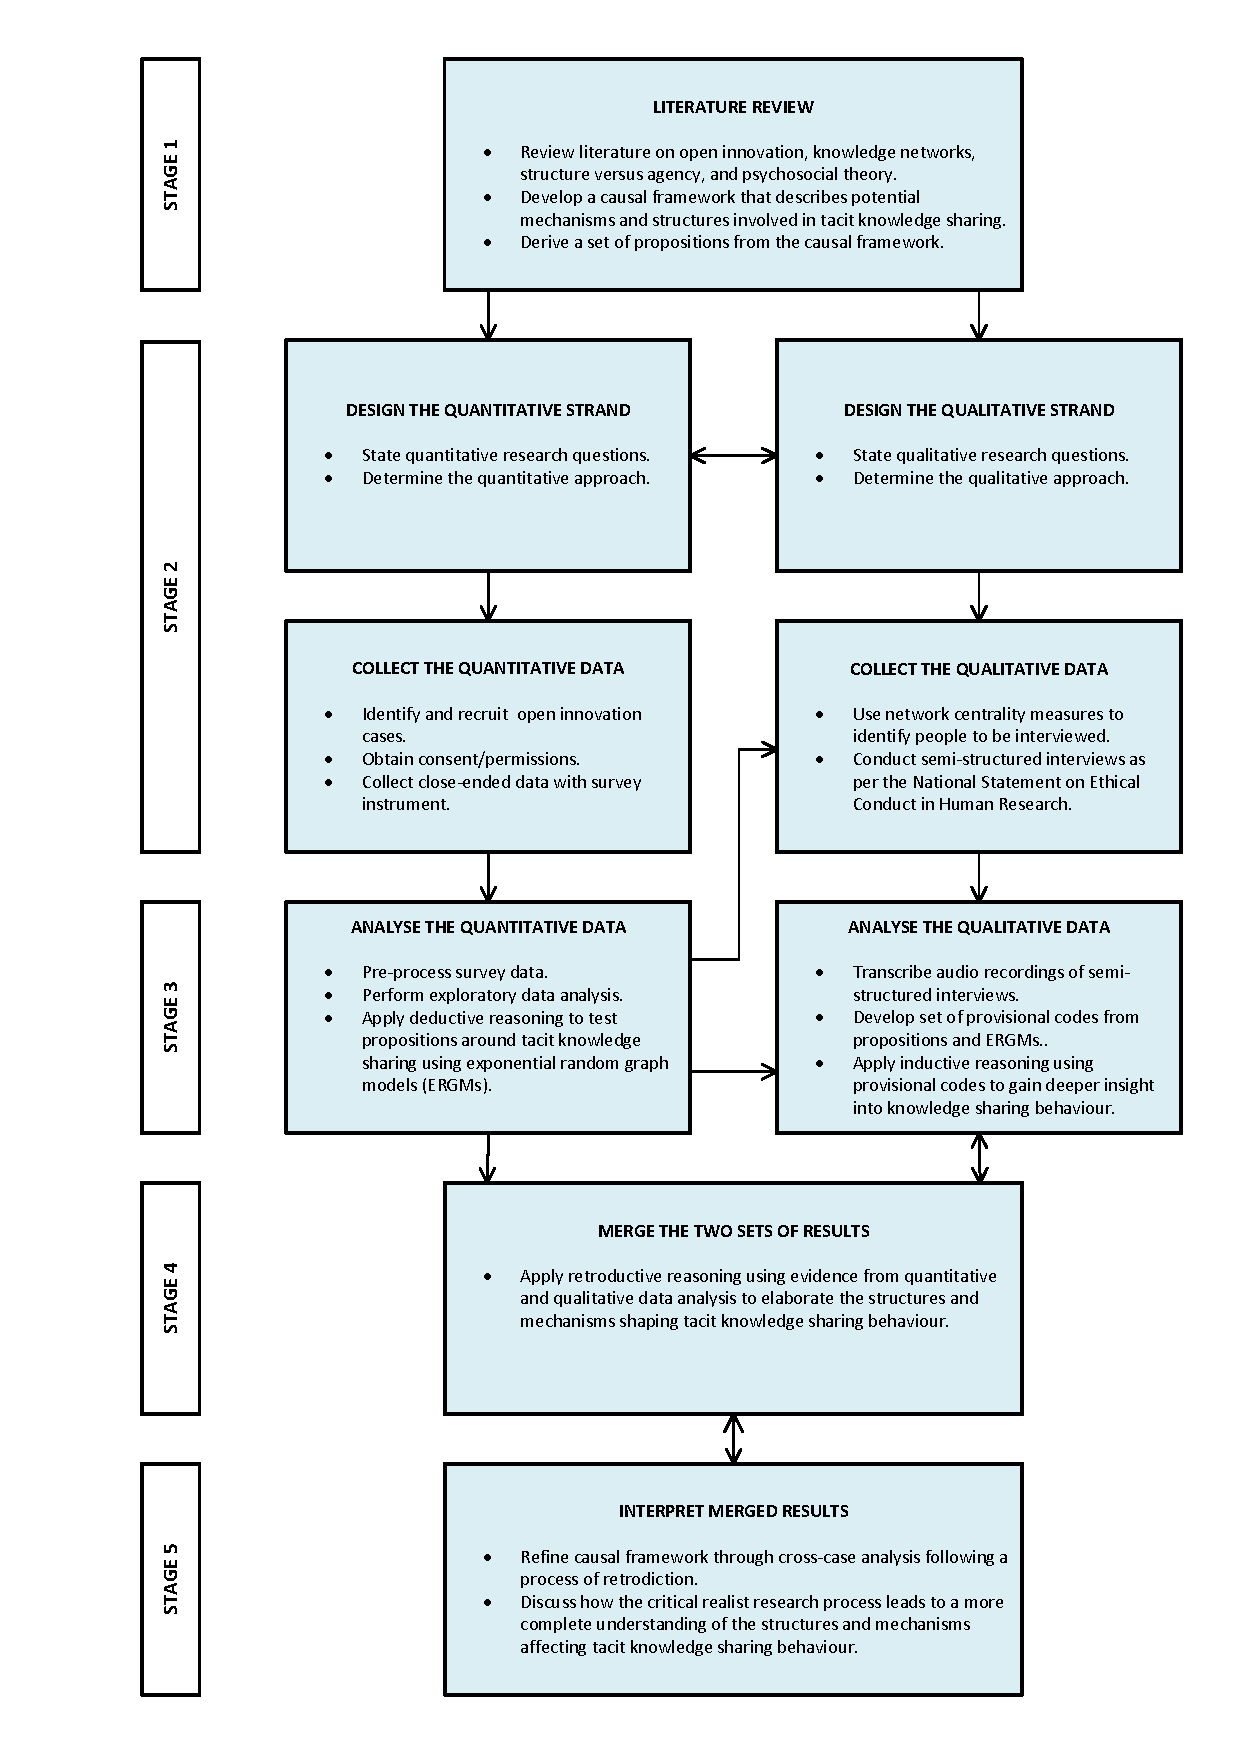
\includegraphics[width = 1.0\textwidth]{Images/mm.pdf}
\caption[Mixed method research design]{Mixed method critical realist research design.}
\label{fig:mm}
\end{figure}

Determining causal mechanisms in social network analysis is difficult because of the confounding nature of endogenous and exogenous network effects \citep{rogowski2012estimating,forastiere2018estimating}. Exponential random graph models (ERGMs) are a class of statistical model for social networks that allow simultaneous testing of multiple hypotheses about network structure and tie formation. Models represent an accumulation of local network configurations (also referred to as subgraphs, motifs, or microstructures) that build the global structure of the network \citep{robins2013tutorial}. Network configurations are assumed to represent underlying social processes or mechanisms \citep{lusher2013exponential}. A combination of social and psychological theories was used to predict purely structural network effects (reciprocity, popularity and activity spread, simple as well as multiple connectivity, transitive closure), actor-relation effects (sender/receiver, homophily), and actor-brokerage effects (different broker roles). While such quantitative analysis can disambiguate potentially confounding network effects, it cannot account for unobserved contextual or experiential factors that may affect network structures in open innovation partnerships. Hence, the next step in the critical realist research process is to apply retroduction to develop a more robust causal framework for each case. In the case of this study, the process of retroduction relied on evidence from the exponential random graph models and semi-structured interviews. It is important to note that with cross-sectional studies, such as this one, there is a limit to what one can infer about causal mechanisms. \medskip

The final step in the critical realist research process involves combining the causal frameworks for each case to create a cross\hyp{}case causal framework. Differences between cases are reconciled using retrodiction to create more robust explanations of mechanisms \citep{mcavoy2018critical}. \medskip

\begin{sidewaystable}
\centering
\caption{}
\label{tab:welch_cases}
\resizebox{\textwidth}{!}{%
\begin{tabular}{@{}lllll@{}}
\toprule
Dimension &
  Inductive theory building &
  Natural experiment &
  Interpretive sense-making &
  Contextualised explanation \\ \midrule
Philosophical orientation &
  Positivist (empiricism) &
  Positivist (falsification) &
  Interpretive/ constructionist &
  Critical realist \\
Nature of research process &
  Objective search for generalities &
  Objective search for causes &
  Subjective search for meaning &
  Subjective search for causes \\
Case study outcome &
  Explanation in the form of testable propositions &
  Explanation in the form of cause-effect linkages &
  Understanding of actor's subjective experiences &
  Explanation in the form of causal mechanisms \\
Strength of case study &
  Induction &
  Internal validity &
  Rich description &
  Causes-of-effects explanations \\
Attitude to generalisation &
  Generalisation to population &
  Generalisation to theory (analytic generalisation) &
  Particularisation not generalisation &
  Contingent and limited generalisations \\
Nature of causality &
  Regularity model: proposing associations between events (weak form of causality) &
  Specifying cause effect relationships (strong form of causality) &
  Too simplistic and deterministic a concept &
  Specifying causal mechanisms and the contextual conditions under which they work (strong form of causality) \\
Role of context &
  Contextual description a first step  only &
  Causal relationships are isolated from the context of the case &
  Contextual description necessary for understanding &
  Context integrated into  explanation \\
Main advocate &
  \citet{eisenhardt1989building} &
  \citet{yin2009case} &
  \citet{stake2005qualitative} &
  \citet{ragin2009reflections,bhaskar2013realist} \\ \bottomrule
\end{tabular}%
}
\end{sidewaystable}[]

\section{Ethics clearance}

As this thesis deals with human participants, it was subject to the ethical guidelines contained in the Australian National Statement on Ethical Conduct in Human Research \citep{national2007national}. Formal ethics approval from both the Commonwealth Scientific and Industrial Research Organisation and Swinburne University of Technology was required before any data could be collected. Approval hinged on individual participants being sufficiently informed to give consent, allowing information about themselves to be used in this study. An application for ethics clearance was submitted to the ethics committees at both organisations. The application included a brief description of this study, a plain language information sheet for participants, a blank consent form, and a list of questions to be included in an online survey. Both committees deemed this study low-risk and allowed the collection and subsequent analysis of data to proceed, subject to standard terms and conditions as per the National Statement on Ethical Conduct in Human Research (the ethics approval may be found in Appendix A). These include alerting both committees to any changes in data collection procedures and reporting any complaints or issues raised by participants. None of the study participants raised any issues with the conduct of this study. 

\section{Research participants}

Finding appropriate candidates for open innovation case studies was challenging. This thesis is part of a broader initiative looking at innovation in the food and agriculture sector. Potential candidates were identified using leads provided by agricultural consultants, university researchers, government agencies, and non-governmental organisations. Most of the firms approached were not that keen on outsiders observing how they went about open innovation. Some firms argued their inter-organisational relationships were a trade-secret and did not want to risk anyone finding out about their strategic or commercial intentions. Other firms felt this study would consume too much their time or be too disruptive to their operations. Ultimately, the recruitment of cases relied on a combination of perseverance and goodwill. Altogether three cases were recruited for this study. 

\section{Quantitative procedures}

\subsection{Data collection}

Each case followed the same procedure for collecting and analysing quantitative data. For each case, the primary contact person (usually the project instigator) was asked to compile a list of people directly involved in the effort. An online survey was employed to collect quantitative data. The survey captured demographic information about respondents, whom they related to in the collaboration, and how they perceive themselves.\medskip

Any missing data impacts negatively on network studies. Hence this study aimed for a 100\% survey response rate. The primary contact person was asked to strongly encourage everybody on their list to participate in this study. 

\subsubsection{Questionnaire design}

The online survey was kept short as an inducement to complete the survey and to avoid responder fatigue \citep{crawford2001web,evans2005value,van2006conducting}. An informal poll among workplace colleagues at the Commonwealth Scientific Industrial Research Organisation (CSIRO) indicated that an online survey should take no longer than 15 or so minutes to complete. With this limitation in mind, the survey questionnaire was designed having three parts. The first part captured demographic information about the respondent, namely their age, gender, occupation, level and field of education, workplace postcode, relevant work experience, and current job tenure. Relevant work experience is essential as this is the primary source of useful tacit knowledge \citep{nonaka1995knowledge,sternberg1999tacit}. Response options for categorical questions were based on the Australian and New Zealand Standard Classification of Occupations \citep{pink2009anzsco} and the Australian Standard Classification of Education \citep{trewin2000australian}. Respondents were also asked to state their role in the open innovation partnership. \medskip

The second part of the questionnaire captured information about specific social relationships. Respondents were asked to name people in the open innovation collaboration they received knowledge and ideas from, felt they could trust, they reported to, and have worked with before (see Figure \ref{ng} for list of the name-generator and name-interpreter questions). \bigskip

\begin{figure}[p]
\centering
\label{ng}
\caption[Name-generator/interpreter questions]{Name-generator (NG) and name-interpreter (NI) questions.}
\begin{tcolorbox}
\begin{itemize}
    \item[\textbf{NG 1}] \textit{Name people who provide you with useful knowledge that helps you accomplish your tasks in this collaboration.}
    \begin{itemize}
        \item[\textbf{NI 1-1}] \textit{How much of the knowledge provided by this person is documented?}
        \item[\textbf{NI 1-2}] \textit{How complex is the knowledge provided by this person?}
        \item[\textbf{NI 1-3}] \textit{How much time does this person spend demonstrating their knowledge to me?}
    \end{itemize}
    \item[\textbf{NG 2}] \textit{Name people who help you come up with new ideas or novel solutions to hard problems in this collaboration.}
    \item[\textbf{NG 3}] \textit{Name people who help you transform ideas into product, process or service concepts for further development and commercialisation in this collaboration.}
    \item[\textbf{NG 4}] \textit{Name people in the collaboration you can share ideas, feelings and hopes with. These are people with whom you have made a considerable emotional investment in your working relationship. You can talk freely with them about the difficulties you are having at work. They will listen and respond in a constructive, caring way. You would share a sense of loss with them if you could no longer work together.}
    \item[\textbf{NG 5}] \textit{Name people in the collaboration you consider professional, competent, and dedicated. You can count on them not to make your job harder by careless work. They have the trust and respect of their colleagues, including those who are not friends.} 
    \item[\textbf{NG 6}] \textit{Name people you formally report to in this collaboration.}
    \item[\textbf{NG 7}] \textit{Name people in this collaboration you have worked and interacted with prior to this collaboration getting underway.}
\end{itemize}
\end{tcolorbox}
\end{figure}

Respondents could select names from a drop-down list or add names of people missing from the list. Asking respondents whom they receive knowledge and ideas from, rather than whom they share knowledge or generate ideas with, was a deliberate move to avoid them nominating everybody in the drop\hyp{}down list. By asking respondents to nominate whom they received knowledge and ideas from required them to think more carefully about their response. Respondents also had to indicate how much of the knowledge provided to them was tacit. Tacit knowledge may be characterised in terms of \enquote{complexity}, \enquote{codifiability}, and \enquote{observability} \citep{winter1987knowledge,zander1995knowledge,cavusgil2003tacit}. Any knowledge that is complex, poorly encoded, and mostly acquired through observation is considered to be predominantly tacit. For each knowledge provider, respondents had to rate how complex was the knowledge provided to them, to what extent was the knowledge documented, and how much direct observation was required to obtain the knowledge on a 10\hyp{}point scale. \medskip 

The third part of the questionnaire aimed to build a psychological profile of the respondent in terms of personality, self-efficacy, organisational identification, and work motivation. Respondents had to rate their level of agreement with several statements about themselves,  using a 10-point scale. Items from an ultra-shortened version of the \enquote{Big Five Inventory} was used to profile personality. The BFI-10 scale uses two items to measure each of the big five personality traits \citep{rammstedt2007measuring}. Only three personality traits positively correlated with knowledge sharing were profiled, namely \enquote{agreeableness}, \enquote{conscientiousness}, and \enquote{openness to experience} \citep{matzler2008personality,matzler2011personality}. While the BFI-10 is reported to be a less reliable scale (agreeableness: $\alpha$ = 0.42, conscientiousness: $\alpha$ = 0.67, emotional stability: $\alpha$ = 0.78, extraversion: $\alpha$ = 0.79, openness: $\alpha$ = 0.50), it is sufficient for research settings with tight time-constraints \citep{rammstedt2007measuring}.\medskip

This study assessed self-efficacy in terms of how competent a person felt about doing their job, their sense of autonomy, and confidence in their ability to come up with creative ideas or solutions. Job competence and autonomy was profiled using statements from the \enquote{Measuring Empowerment Scale} \citep{spreitzer1995psychological}. Reported reliability of this scale is considered good (job competence: $\alpha$ = 0.81, self-determination: $\alpha$ = 0.81). The ability to come up with creative ideas or solutions was profiled using statements from the \enquote{Creative Self\hyp{}Efficacy Scale} \citep{tierney2002creative}. Past studies indicate this scale is reliable with reported $\alpha$ values between 0.74 and 0.91 \citep{tierney2002creative,gong2009employee,tierney2011creative,mittal2015transformational}.\medskip

The \enquote{Organisational Identification Scale} \citep{mael1992alumni} was used to assess how strongly the respondent identified with his or her work\hyp{}group, employer, and with the open innovation partnership. This scale has proved to be reliable in a variety of study settings with reported $\alpha$ values between 0.73 and 0.89 \citep{mael1992alumni,bergami2000self,knippenberg2000foci,van2008interactive}. Only one of the six items from the scale was used in this survey: \enquote{When someone criticises my organisation, it feels like an insult}. This item has the highest factor loading of all six items \citep{mael1992identifying} and was adapted to address identification with one's work-group, with one's employer, and with the partnership. Using all six items for each of these cases would have been impractical, given the time constraint in which to complete the survey. \medskip

Work motivation was measured using the 19-item \enquote{Multidimensional Work Motivation Scale} \citep{gagne2015multidimensional}. This scale is based on self-determination theory and has sub-scales for amotivation, extrinsic material regulation, extrinsic social regulation, introjected regulation, identified regulation, and intrinsic motivation. Reliability of the English version is good, with reported $\alpha$ values between 0.79 and 0.90. Items in the Multidimensional Work Motivation Scale were modified to suit the study context. For example, the scale has a stem question: \enquote{Why do you or would you put efforts into your current job?}. One response option is: \enquote{Because I personally consider it important to put efforts into this job}. This response was modified to read as thus: \enquote{I put effort into this collaboration because I personally consider it important to do so}. 

\subsubsection{Piloting of the survey}

For quality assurance, the online survey was piloted twice to check if questions were clear and not ambiguous and to establish how long it would take to complete an online survey. Ten people were involved in each pilot (the first pilot involved CSIRO colleagues, the second involved members of the Social Network Research Laboratory at Swinburne University of Technology). Apart from one question about trust, everybody in the first pilot reported no issues with clarity or ambiguity. One person felt the question asking respondents to name people in the partnership they trust was too judgemental. The question was subsequently modified to be less judgemental. Everybody involved in the second pilot was comfortable with the survey, although one person felt the invitation email was too long. Most of the people in each pilot completed the survey within 20 minutes. The only exceptions were people who took their time making detailed notes as they went through the survey. Table \ref{tab:self-report} in Appendix B lists the 59 items used in the online survey, together with associated response options and references.

\subsubsection{Survey procedure}

The list of people involved in each open innovation partnership also included their email addresses. Everybody on the list received an email invite to complete the web-based survey questionnaire. The email provided information about the study and included a unique link to the survey website (\url{http://www.onasurveys.com}). People could either ignore the email invitation or agree to take part in the survey by clicking on the URL link provided. Clicking on the URL link directed them to the survey website where they were asked to give consent to allow their responses to be used in this study. They could not progress with the online survey until consent was given.

\subsection{Social network analysis}

\subsubsection{Key concepts}

A social network is a way to conceptualise a social system in terms of the structure of relationships among social actors. Typically, a social network is represented as a mathematical graph with vertices and edges. Vertices represent actors (also referred to as nodes) and edges the ties (social connections or relations) between them (Figure \ref{fig:examples}). \medskip

\begin{figure}
    \centering
    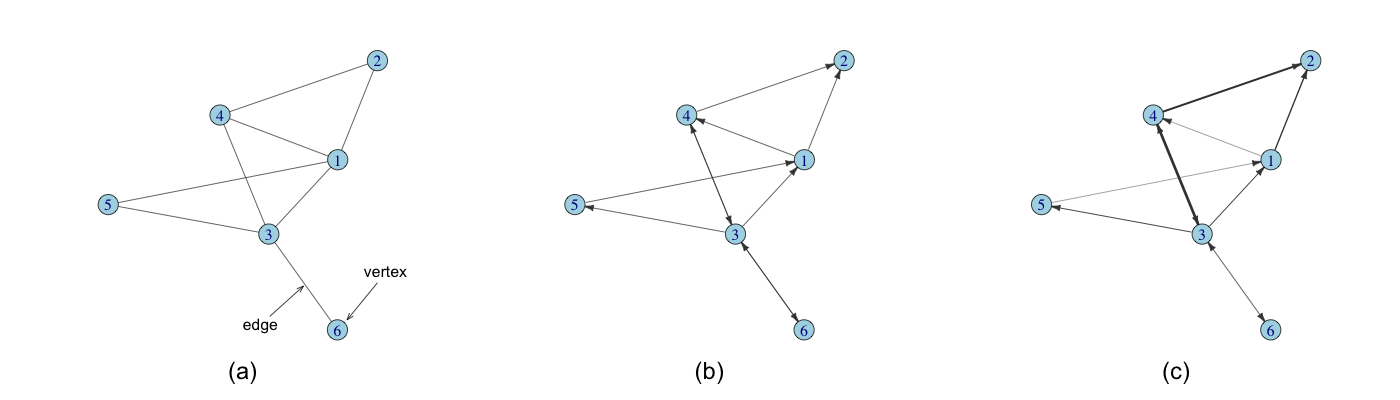
\includegraphics[width=1.0\linewidth]{Images/example_networks.png}
    \caption[Example networks]{Example network with (a) undirected binary ties, (b) directed binary ties, and (c) valued ties (edges are weighted according to some value).}
    \label{fig:examples}
\end{figure}

Actors may be distinguished using any combination of binary, categorical or continuous attributes. For example, consider an individual actor classified as female (binary attribute), who works for a particular organisation (categorical attribute), with a specific number of years of work experience (continuous attribute). Ties between actors can be measured as directed or undirected, and as binary or valued. Deciding whether to measure a tie as directed or undirected depends on the nature of the tie. For instance, ties indicating organisational affiliation are usually undirected, whereas authority is inherently directed \citep{borgatti2013analyzing}. \medskip
 
 A similarity tie is a type of continuous tie that shows a relation between two actors who share something in common (e.g. work at the same location, are affiliated to the same body, participate in the same event, or share a common attribute). Actors can have many different kinds of social relations, e.g. friendship, knowledge sharing, advice seeking, and reporting ties. Relational ties can also be affective (like or dislike another actor) or perceptual (belief about the other actor). Discrete ties refer to ties defined by specific social interactions (e.g. a transaction of some kind, attendance at the same event) and flows (e.g. communication or knowledge flows). \medskip

Ties are often interdependent insofar as the presence of one tie affects the presence of others. Without some form of dependence among ties, it is often difficult to explain the existence of specific social relations \citep{lusher2013exponential}. An example is a friendship tie, which usually develops in the presence of a pre-existing similarity tie (e.g. both actors share a common interest or work at the same place) or via an interaction tie (e.g. actors were introduced to each other at a specific event or worked together on a particular project). \medskip

\begin{figure}
    \centering
    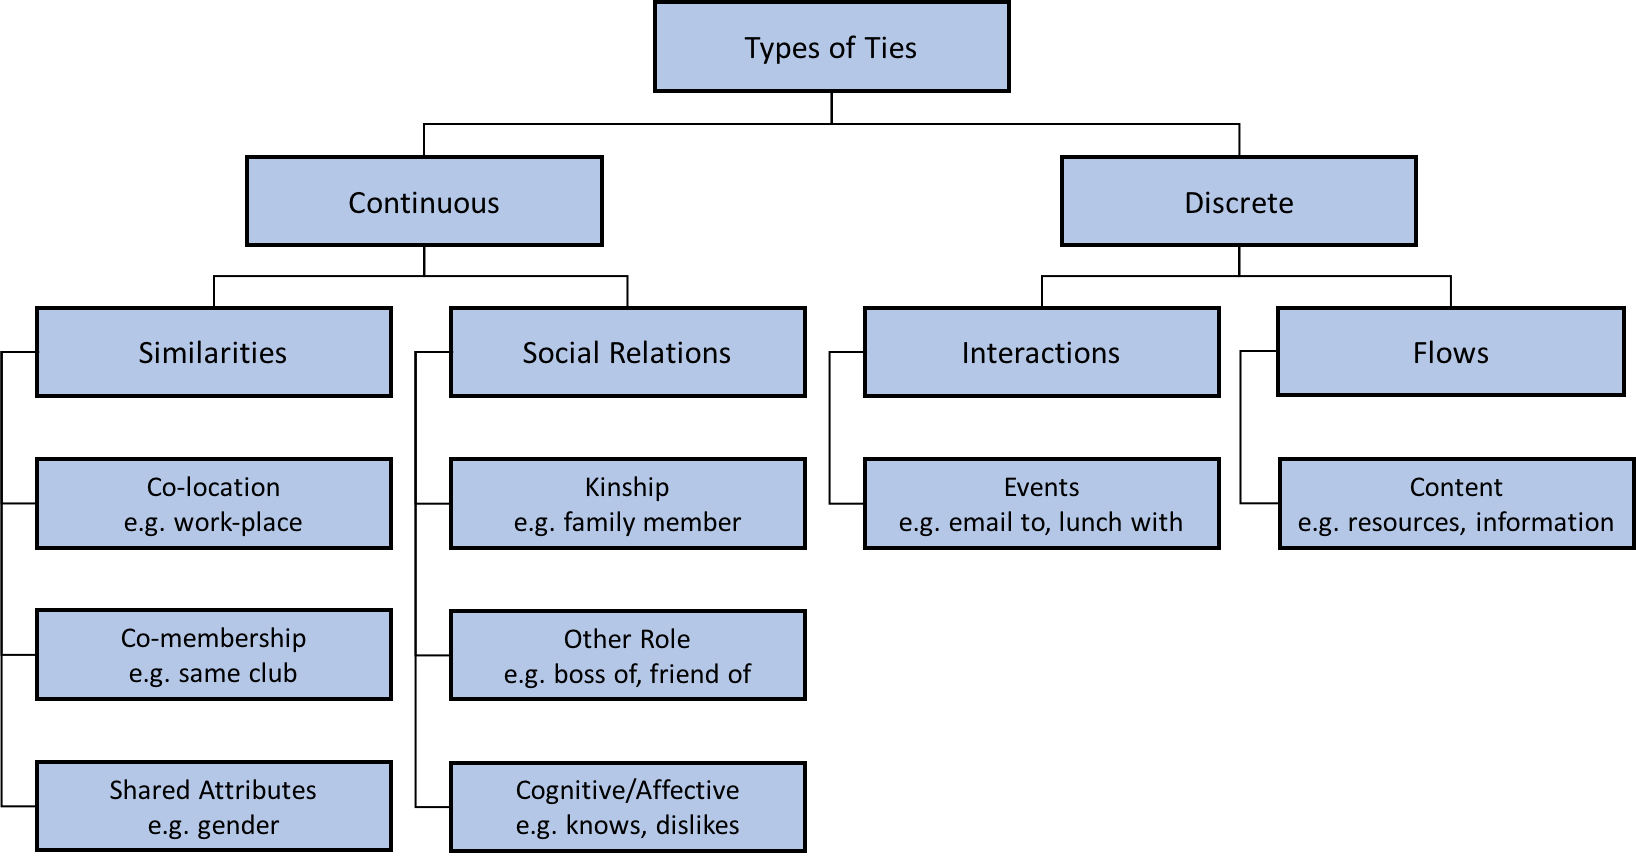
\includegraphics[width=0.9\linewidth]{tie_type}
    \caption[Different types of social ties]{Different types of social ties \citep{borgatti2013analyzing}.}
    \label{fig:tie_type}
\end{figure}

\subsubsection{Network data structures}

Edge lists and adjacency matrices are the most commonly used data structures for social networks. With an edge list, an edge between two actors $i$ and $j$ is denoted as $(i,j)$, so that a complete network with $n$ actors can be specified by giving the value $n$ and a list of edges. The edge list for the undirected binary network depicted in Figure \ref{fig:examples} would have $n = 6$ actors and edges $(1,2),(1,3),(1,4),(1,5),(2,4),(3,4),(3,5),(3,6)$. A directed network has twice the number of total possible edges than an undirected network (directed network edges can be bi-directional). Thus, the edge list for the directed binary network depicted in Figure \ref{fig:examples} would have $n = 6$ actors and edges $(1,2),(1,4),(3,1),(3,4),(3,5),(3,6),(4,2),(4,3),(5,1),(6,3)$. Although edge lists are an efficient way to represent networks, they are too cumbersome for computational operations \citep{newman2010networks}.

An adjacency matrix is a more efficient way to represent and manipulate social network data \citep{hummon1990computational}. For a social network, $X$, the adjacency matrix would be a $n \times n$ matrix with elements $X_{ij}$ representing how actor $i$ is tied to actor $j$. In the case of a binary network, the adjacency matrix is expressed as follows: 
\[
X_{ij} =
\begin{cases}
    1 & \text{if  } i \rightarrow j \\
    0 & \text{otherwise}
\end{cases}
\]
For an undirected network, $X_{ij}$ and $X_{ji}$ are equal. With a directed network, $X_{ij}$ and $X_{ji}$ are treated as different variables, either with the same or different values. For a directed binary network, values = 1 in the $i$th row of an adjacency matrix represent ties sent by actor $i$, and the values = 1 in the $j$th column of an adjacency matrix represent ties received by actor $j$. The adjacency matrix representing both the directed and undirected binary networks depicted in Figure \ref{fig:examples} would be expressed as: \bigskip
$$
X_{ij} =
\left \{
  \begin{tabular}{cccccc}
    0 & 1 & 0 & 1 & 0 & 0 \\
    0 & 0 & 0 & 0 & 0 & 0 \\
    1 & 0 & 0 & 1 & 1 & 1 \\
    0 & 1 & 1 & 0 & 0 & 0 \\
    1 & 0 & 0 & 0 & 0 & 0 \\
    0 & 0 & 1 & 0 & 0 & 0
  \end{tabular}
\right \}
$$ \medskip

In the case of non-binary or valued networks, the presence of a tie is indicated by some value (usually a real number, not equal to 0) that describes a property of the tie e.g. geographic proximity.

\subsubsection{Types of social network analysis}

Social network analysis aims to detect and interpret patterns of social ties between actors \citep{de2011exploratory}. Three core assumptions about patterned relations and their effects underpin social network analysis. First, structural relations are more important than actor attributes for understanding behaviour. For instance, an actor may be well-qualified to perform a specific task but is unable to do the task because the requisite relationships are not in place. Second, social networks shape and are shaped by the perceptions, beliefs, and actions of actors. Third, network structures are dynamic and continually evolving \citep{knoke2008social}. \medskip

Social network analysis can be either egocentric or socio-centric. Egocentric network analysis focuses on the structure of an actor's immediate network (the ego's network) and what this means for that actor \citep{chung2005exploring}. In contrast, socio-centric network analysis considers patterns of social interaction between all the actors in a predefined and bounded population \citep{provan2007interorganizational}. \medskip

This thesis used both descriptive and statistical network analysis techniques to analyse the socio-centric network structure of the three open innovation partnerships. The descriptive network analysis measured the centrality of actors and their brokerage roles in each open innovation partnership. This information was used to identify a subset of actors for follow-up semi-structured interviews (the subset included highly central as well as peripheral actors). The statistical network analysis used exponential random graph models (ERGMs) to examine the interdependence of knowledge sharing ties.

\subsubsection{Brief history of ERGMs}

Traditional methods for analysing social networks are primarily descriptive and not statistical in the sense of modelling random variation in how ties are formed among actors in a network \citep{harris2013introduction}. \citet{erdos1959random} formulated a simple random graph in which the proportion of observed ties out of all possible ties determines the probability of a tie forming between two actors. Simple random graphs are not very good at capturing observed network structures as they do not account for the social forces that influence tie formation \citep{harris2013introduction}. This led  \citet{holland1981exponential} to introduce a random graph model for directed graphs, where the probability of tie formation varies among actors according to their propensity to extend ties to other actors, and the propensity to have ties extended to them by other actors (referred to as a $p_1$ model). \medskip

While this was an improvement over simple random graphs, $p_1$ models do not reflect the interdependence among nodes (e.g. homophily and transitivity effects). Consequently,  \citet{frank1986markov} introduced a new generation of random graph model that assumes a form of dyadic dependence when ties do have actors in common (the Markov dependence assumption). Although it incorporated more of the structural characteristics found in observed networks, the model introduced by \citet{frank1986markov} does not include node attributes as covariates. \medskip

A major breakthrough came when \citet{wasserman1996logit} introduced a new model that assumes a more general conditional dependence between ties. Essentially, this model assumes the likelihood of any two ties existing at the same time is different from the combined likelihood of each tie being present. Their model allows for multiple dependence assumptions at both dyadic and node level(hence these models are referred to as $p^*$ models). \medskip

Statistically, an ERGM represents a probability distribution of graphs for a given set, where the probability of observing a graph is dependent on the presence of the various network configurations expressed by the model. Importantly, the unit of analysis in an ERGM is not the number of nodes, but the number of possible ties between all actors in the network ($n(n-1)$). Even with a small number of actors, an ERGM has sufficient statistical power to make inferences about how ties are formed \citep{lusher2013exponential}. \medskip

For a binary network, the probability of observing specific network configurations for a given set of actors \(n\) can be expressed as follows: $$ P(X = x) = \frac{\exp \left \{ \theta'z(x)  \right \}}{\kappa (\theta )} $$ where $P(x)$ indicates the probability of a given network, $\theta$ indicates a vector of model parameters, $z(x)$ is a vector of network statistics, and $\kappa$ is a normalising function to ensure a proper probability distribution across a set of random networks \citep{shumate2010exponential}. Network statistics $z(x)$ are counts of the estimated number of configurations in the network, or some function of those counts. The probability of the network depends on how many of those configurations are present and the parameters indicate the importance of each configuration \citep{lusher2013exponential}. Large positive parameters suggest that more configurations of that type are observed in the network than expected by chance alone \citep{robins2009closure}. \medskip

ERGMs are theory-driven in that their use requires the researcher to consider the complex, intersecting, and often competing theoretical reasons why particular social ties in the observed network exist \citep{lusher2013exponential}. For instance, does a given network structure occur due to processes of homophily, reciprocity, transitivity, or through a combination of these? By including such parameters together in one model, a researcher can test certain hypotheses or propositions about tie formation relating to theory \citep{robins2007recent}. ERGMs can distinguish between ties formed due to actor attributes or whether an actor’s centrality is the result of being embedded within other purely structural network structures \citep{lusher2013exponential}. Purely structural effects reflect self-organising or endogenous processes where ties form due to the presence or absence of other ties, e.g. reciprocity and transitive closure. Actor-relation effects refer to ties that form due to actor attributes. Homophily is an example of an actor-relation effect. Dyadic covariate effects refer to ties in one network being affected by ties in another network. A good example is the geographic separation between actors, which may affect the formation of relationships between them. Another example is advice seeking, which is more likely to occur in the presence of an existing friendship tie. \medskip

Alternative methods used to assess the effect of actor attributes on network structures, such as linear regression, are unable to make such distinctions and are thus more limited regarding the conclusions such methods can draw. One limitation of ERGMs is that the algorithms used to estimate model parameters often fail to converge (i.e. are unable to produce a stable set of parameter estimates). For this reason, ERGMs tend to be parsimonious, including only the most important configurations needed to answer specific research questions \citep{mcallister2017balancing,silk2017application}. 

\subsubsection{Data pre-processing}

The first step was to retrieve survey responses for each case from the \texttt{ONASurveys} website. Each case had its own Microsoft Excel\texttrademark\ workbook with two worksheets. The first worksheet contained demographic information about each respondent and their responses to the personality, self-efficacy, organisational identification, and work motivation scale items. The second worksheet listed for each respondent their nominated sources of knowledge and ideas, people they work with to realise ideas, trusted others, line or project managers, and individuals with whom they have previously worked. \medskip

Various \texttt{R} packages were used to pre-process data for social network analysis, generate network diagrams, and perform descriptive network analysis. These are listed in Appendix C (Table \ref{tab:r_packages}). \texttt{R} is a popular cross-platform open-source software system for statistical computing \citep{core2018r}. Readers can access the \texttt{R} scripts used to pre-process, analyse and visualise data at \url{http://github.com/aterhorst/phd}. The exponential random graph modelling was done using \texttt{MPNet}, a Microsoft Windows\texttrademark\ application for statistical network analysis \citep{wang2014mpnet}. \medskip

Survey responses were loaded into \texttt{RStudio}, a free and open-source integrated development environment (IDE) for \texttt{R}, as two separate tabular data sets (i.e. a node table listing personal information about each respondent, and an edge table listing the different ways respondents relate to each other). The first step in the data tidying process involved fixing minor data-entry errors in the node table. Once data-entry errors were eliminated, the next step involved aggregating the personality, self-efficacy, organisational identification, and work motivation scale items. Aggregated scale items were re-scaled to be a fractional number between 0 and 1. \medskip

Respondents had to qualify the type of knowledge provided to them in terms of its complexity, observability, and level of encoding \citep{winter1987knowledge,zander1995knowledge,cavusgil2003tacit}. Knowledge sharing relations were valued on a scale of 0 to 1 by aggregating and re-scaling the three criteria to come up with a measure of knowledge tacitness. This allowed knowledge sharing relations to be split into two types, i.e. predominantly tacit and predominantly explicit knowledge sharing relations. Predominantly tacit knowledge (tacitness $> 0.5$) lacks documentation, is likely to be complex, and mostly acquired through observation. Predominantly explicit knowledge (tacitness $< 0.5$), on the other hand, tends to be well-documented, is not particularly complex, and requires little demonstration to be communicated. Although the edges of the predominantly tacit and a predominantly explicit knowledge network do not overlap, this thesis does not treat knowledge as a binary construct (as either completely tacit or totally explicit knowledge). This thesis assumes all knowledge has a tacit component. It uses a simple majority rule to differentiate knowledge according to its level of tacitness. \medskip

A multilayer network object was generated from the tidied node and edge data. Each layer in the network object represents a different set of relationships (tacit and explicit knowledge provider, idea contributor, cognition-based trust, affect-based trust, reporting, and historical relations). Given the survey asked respondents to name people in the partnership who (a) provided them with useful knowledge, and (b) contributed ideas to help them solve problems, the edges in both the knowledge provider and idea contributor layers were reversed to indicate the flow of knowledge and ideas. \medskip

The survey questionnaire asked respondents to enter their workplace postcodes. Geographic coordinates (longitude and latitude) were derived for each postcode using the \texttt{ggmap} package (the \texttt{geocode} function uses the Google Maps\texttrademark\ application programming interface (API) to do this). The spherical (also known as the \enquote{great circle}) distance between all survey respondents could then be calculated using the \texttt{geosphere} package (distances were expressed in kilometres). This information was added as an edge attribute in each network layer. \medskip

Adjacency matrices and corresponding node attributes were extracted from the multi-layer network object and saved as ASCII text files for exponential random graph modelling in \texttt{MPNet}. Apart from the valued adjacency matrix representing geographic separation between nodes (values = $log_e(\text{spherical distance(km)} + 1)$ between nodes), the adjacency matrices were binary in nature (0 = no edge between nodes, 1 = edge between nodes). 

\subsubsection{Exploratory data analysis}

The first thing to do with any survey data set is to get to know it. Not only does this allow one to become familiar with the data, it also helps reduce the workload during analysis \citep{cox2017translating}. Exploratory data analysis is about finding trends in the data, not so much about the strength of the evidence \citep{morgenthaler2009exploratory}. Usually, this involves applying various data visualisation techniques to explore the content and structure of the survey data. Insights gained from exploratory data analysis can help refine research questions, strengthen hypotheses, and improve model specifications \citep{jebb2017exploratory}. \medskip

Exploratory data analysis was used to assess responses to the survey scale items, check for significant correlations between survey items, profile the demographics of each case, and highlight central actors who provide and receive tacit and explicit knowledge as well as ideas in each case. Checking for a significant correlation between survey items involved combining the node tables for all three cases (to get a reasonable sample size). A correlation matrix was generated for the aggregated scale items using the \texttt{cor} function in the base \texttt{R} package. Significant correlations were visualised using the \texttt{corrplot} package in R \citep{wei2017corrplot}. Apart from highlighting interesting correlations between aggregated scale items, results from the correlation analysis helped guide the selection of actor attributes for the exponential random graph models. The graphical data analysis focused on the demographics of each case. This analysis included generating box-plots of age, job tenure, and work experience of actors (continuous variables) and rose-diagrams showing their level and field of education (categorical variables) using the \texttt{ggplot2} package in \texttt{R} \citep{wickham2016ggplot2}. Network diagrams depicting the predominantly tacit and predominantly explicit networks were generated using the \texttt{ggraph} package in \texttt{R} \citep{pedersen2019ggraph}. Nodes were sized according to their respective \enquote{Everett-Valente} brokerage scores \citep{everett2016bridging}. Edges were weighted according to the geographic distance between connected node pairs (expressed as $log_e(\text{spherical distance(km)} + 1)$). 

\subsubsection{Descriptive network analysis} \label{sss:descriptive_network_analysis}

The descriptive network analysis measured various centrality measures, namely in-degree, out-degree, and betweenness centrality for each actor in the tacit and explicit knowledge provider networks \citep{freeman1979centrality}. Also measured was the Everett-Valente brokerage score for each actor \citep{everett2016bridging}. The descriptive network analysis also measured the frequency of the five \citet{gould1989structures} broker roles in each network. \medskip 

In-degree centrality measures the number of ties directed towards an actor whereas out-degree centrality measures the number of ties directed away from an actor. Given the adjacency matrix of a directed network has the element $A_{ij} = 1$ for an edge from $j$ to $i$, in- and out-degrees can be expressed as: $$CD_i^{in} = \sum_{j = 1}^nA_{ij}, \,\,\,\,\,\, CD_j^{out} = \sum_{i = 1}^nA_{ij}$$ \noindent Put differently, in-degree centrality is the sum of column $j$ and out\hyp{}degree centrality is the sum of row $i$ in adjacency matrix $A_{ij}$ \citep{newman2010networks}. In-degree centrality is an indicator of an actor's ability to acquire knowledge, whereas out-degree centrality is an indicator of an actor's knowledge sharing activity. Betweenness centrality measures the extent to which an actor lies on paths between other actors: $$ CB_i=\sum_{i < k}\frac{g_{jik}}{g_{jk}} $$ where $b_i$ is the betweenness centrality for actor $i$, $g_{jik}$ is the number of shortest paths connecting $j$ and $k$ through $i$, and $g_{jk}$ is the total number of shortest paths connecting $j$ and $k$ \citep{freeman1979centrality}. Actors with high betweenness centrality are well\hyp{}positioned to control the flow of information or resources in a network \citep{everett2016bridging}. However, network size moderates the ability of actors to control information and resource flows (larger networks offer more alternative paths, limiting the control of actors). Hence, this study uses a modified betweenness centrality measure known as the \enquote{Everett-Valente} brokerage score that accounts for network size and isolated nodes \citep{everett2016bridging}. In the case of a directed network, as long as $CB_i \neq 0$, the incoming and outgoing Everett-Valente brokerage scores are calculated as follows: \medskip

$$\textit{in-EV-brokerage}_i = \frac{CB_i + j}{CD_i^{in}},  \,\,\,\,\,\, \textit{out-EV-brokerage}_i = \frac{CB_i + k}{CD_i^{out}} $$ \medskip

\noindent where $j$ is the number of vertices that can reach vertex $i$, and $k$ is the number vertices that $i$ can reach. Nodes depicted in the network diagrams were sized using the average of the incoming and outgoing brokerage measures: \medskip

$$ \textit{EV-Brokerage}_i = \frac{\textit{in-EV-Brokerage}_i + \textit{out-EV-Brokerage}_i}{2} $$ \medskip

To compute \citet{gould1989structures} broker roles, the tacit and explicit knowledge networks were extracted from the multi-layer network object and saved as a separate \texttt{network} objects \citep{butts2008network} using the \texttt{intergraph} package \citep{bojanowski2015intergraph}. The \texttt{brokerage} function in the R \texttt{sna} package \citep{butts2016sna} was then used to tally broker roles in each network. 

\subsubsection{Statistical network analysis}

The statistical analysis comprised two sets of ERGM estimations per case. One set of estimations tested propositions about the role of motivation, trust, and power in tacit and explicit knowledge exchanges, while the other set of estimations examined the significance of different broker roles in each case. The choice of which actor\hyp{}relation effects to include in the first set of models was guided by the propositions and exploratory analysis. \citet{gould1989structures} estimated the statistical significance of their five broker roles using a simple $p_1$ model. Their approach does not account for other possible network effects and tie dependencies that are likely to produce distorted results. Modifications were made to \texttt{MPNet} to allow the statistical significance of the different broker roles to be estimated more accurately. The modified software was used in the second set of model estimations to characterise the three open innovation partnerships in terms of the mix of significant broker roles. Table \ref{tab:ergm_params} lists the model parameters used in this study. \medskip

\begin{table}[!htbp]
\centering
\resizebox{\textwidth}{!}{%	
\begin{threeparttable}
\footnotesize
\setlength{\tabcolsep}{6pt}
\renewcommand{\arraystretch}{1}
\caption[Exponential random graph model parameters]{Exponential random graph model parameters used in this study.}
\label{tab:ergm_params}
\begin{tabular}{lcl}
\toprule
\textbf{Parameter} & \textbf{Graphic} & \textbf{Explanation}  \\ \midrule
\textbf{Purely structural effects} & & \\
Arc (edge) & \begin{minipage}{.2\textwidth} \centering 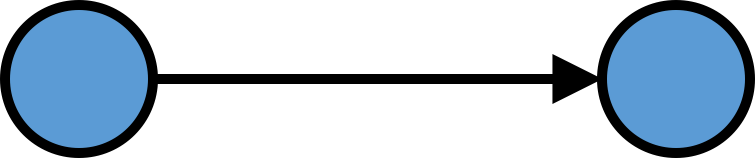
\includegraphics[width=0.4\linewidth]{Images/Arc} \end{minipage} & \begin{tabular}[c]{l}Baseline tendency for a tie to form\\ effects.\end{tabular} \\ \\
Reciprocity (mutuality)	& \begin{minipage}{.2\textwidth} \centering 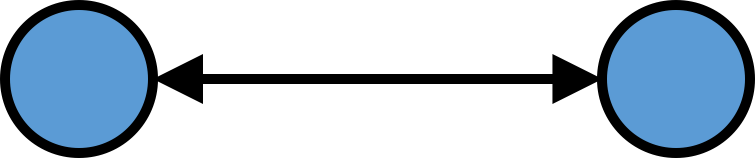
\includegraphics[width=0.4\linewidth]{Images/Reciprocity} \end{minipage} & \begin{tabular}[c]{l}Tendency for a tie from one actor to a second when there\\ is already a tie from the second to the first.\end{tabular} \\ \\ TwoPath (simple connectivity) & \begin{minipage}{.2\textwidth} \centering 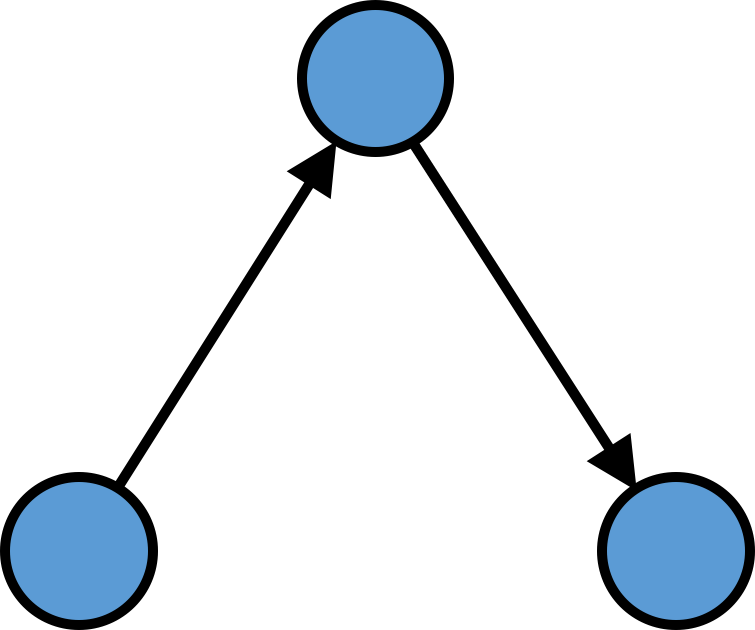
\includegraphics[width=0.4\linewidth]{Images/TwoPath} \end{minipage} & \begin{tabular}[c]{l}Tendency for ties to form as part of simple path formations. \end{tabular} \\ \\
AinS (popularity spread) & \begin{minipage}{.2\textwidth} \centering 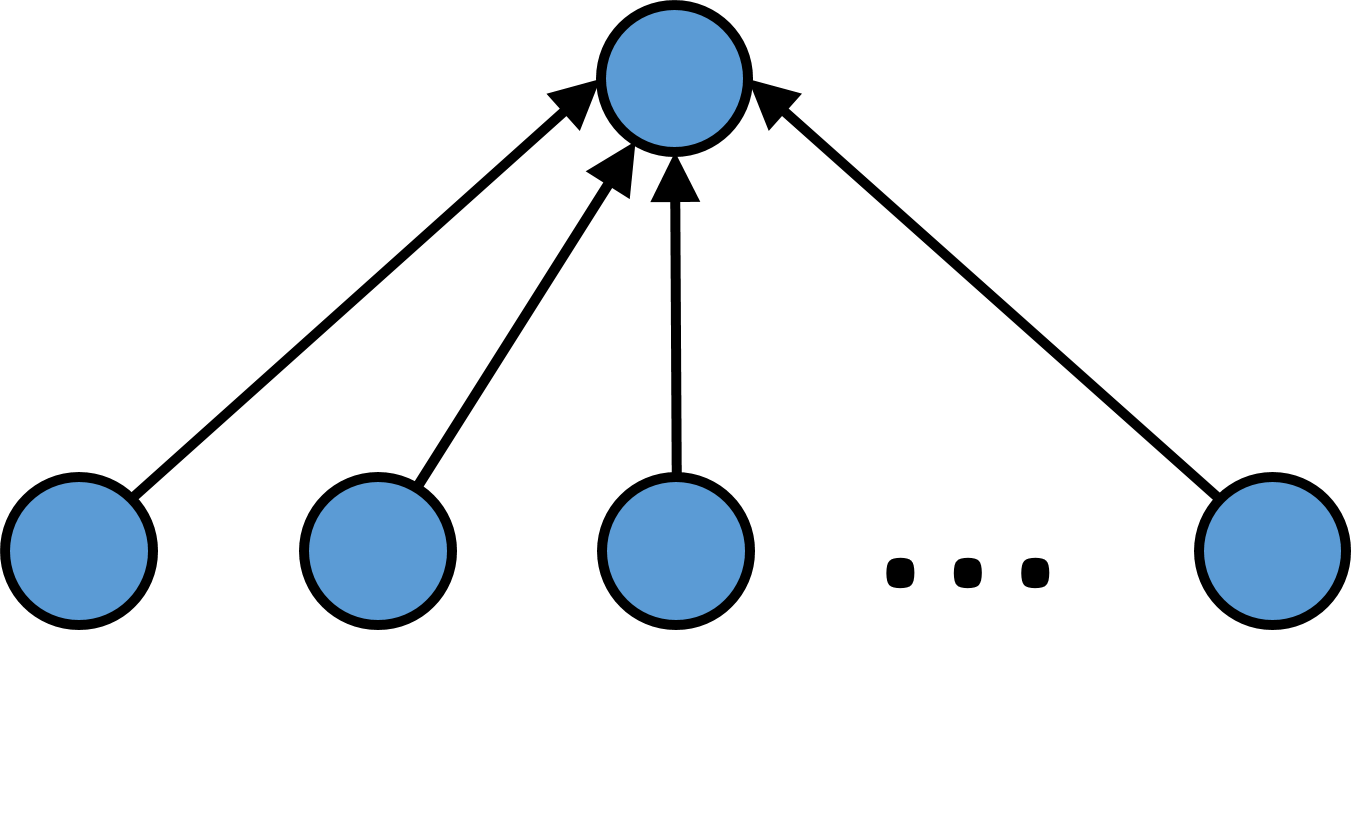
\includegraphics[width=0.6\linewidth]{Images/AinS} \end{minipage} & \begin{tabular}[c]{l}Propensity for dispersion in the in-degree distribution,\\ indicating there are a few highly popular actors. \end{tabular} \\ \\
AoutS (activity spread) & \begin{minipage}{.2\textwidth} \centering 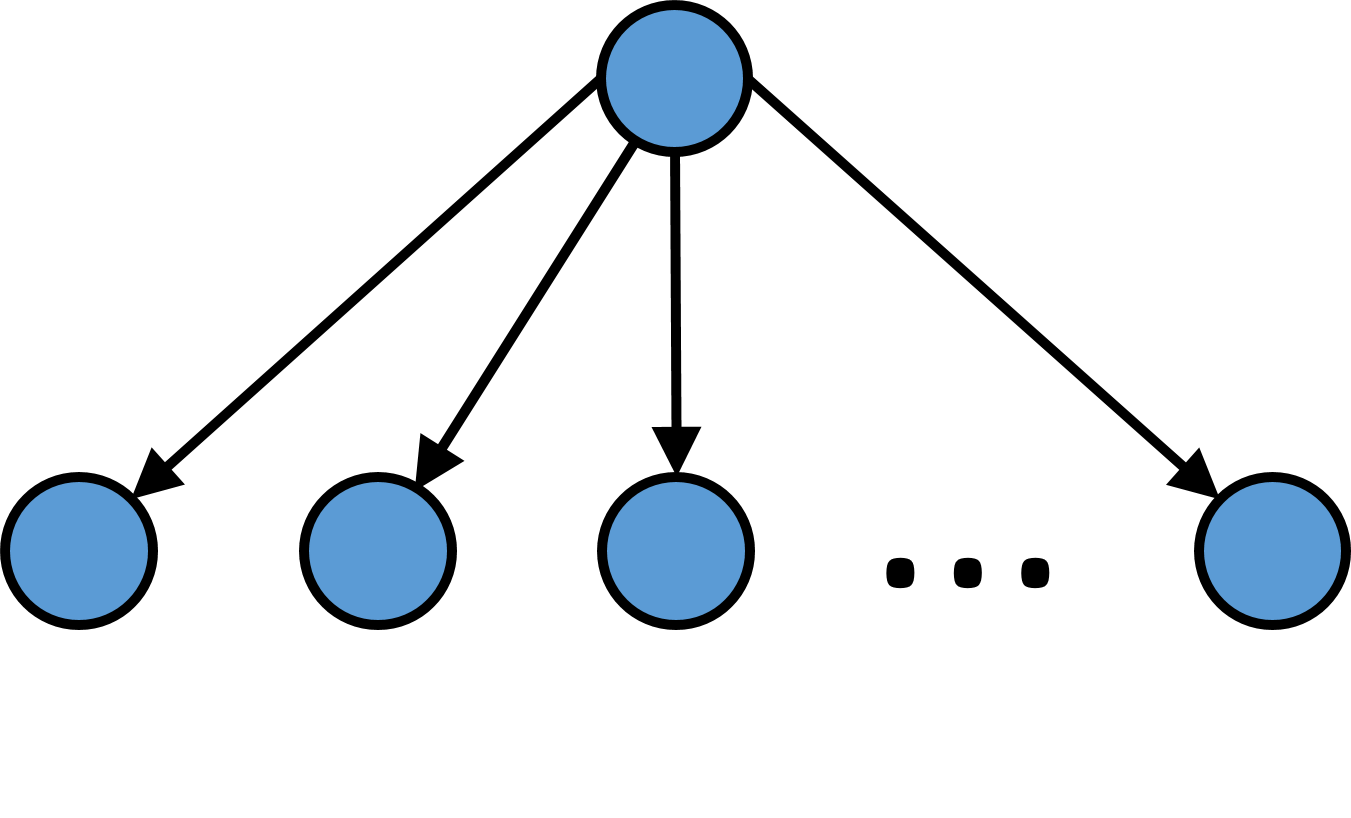
\includegraphics[width=0.6\linewidth]{Images/AoutS} \end{minipage} & \begin{tabular}[c]{l}Propensity for dispersion in the out-degree distribution,\\ indicating there are a few highly active actors. \end{tabular}  \\ \\
AT-T (path closure) & \begin{minipage}{.2\textwidth} \centering \includegraphics[width=0.6\linewidth]{Images/AT-T} \end{minipage} & \begin{tabular}[c]{l}Propensity for ties to form as part of transitive triad or a\\ multiple transitive configuration. \end{tabular} \\ \\
A2P (multiple connectivity) & \begin{minipage}{.2\textwidth} \centering \includegraphics[width=0.6\linewidth]{Images/A2P} \end{minipage} & \begin{tabular}[c]{l}Propensity for ties to form as part of formations involving\\ multiple short paths between actors. \end{tabular} \\ \\
\textbf{Actor-relation effects} & & \\
Attribute sender & \begin{minipage}{.2\textwidth} \centering \includegraphics[width=0.4\linewidth]{Images/Sender} \end{minipage}	& \begin{tabular}[c]{l}Propensity for a tie to be directed from an actor with a\\ particular attribute. \end{tabular} \\ \\
Attribute receiver & \begin{minipage}{.2\textwidth} \centering \includegraphics[width=0.4\linewidth]{Images/Receiver} \end{minipage} & \begin{tabular}[c]{l}Propensity for a tie to be directed toward an actor with a\\ particular attribute. \end{tabular} \\ \\
Attribute difference & \begin{minipage}{.2\textwidth} \centering \includegraphics[width=0.4\linewidth]{Images/Difference} \end{minipage} & \begin{tabular}[c]{l}Propensity for a tie to form between actors with a similar\\ continuous attribute. \end{tabular} \\ \\
Attribute match & \begin{minipage}{.2\textwidth} \centering \includegraphics[width=0.4\linewidth]{Images/Match} \end{minipage} & \begin{tabular}[c]{l}Propensity for a tie to form between actors with the same\\ categorical attribute.\end{tabular} \\ \\
Attribute mismatch reciprocity & \begin{minipage}{.2\textwidth} \centering \includegraphics[width=0.4\linewidth]{Images/MisMatchReciprocity} \end{minipage} & \begin{tabular}[c]{l}Propensity for a tie to form between actors with a\\ non-matching categorical attribute.\end{tabular} \\ \\
\textbf{Actor-brokerage effects} & & \\
b\textsubscript{O} (liaison role) & \begin{minipage}{.2\textwidth} \centering \includegraphics[width=0.4\linewidth]{Images/b_O} \end{minipage} & \begin{tabular}[c]{l}Propensity to have brokers who mediate communication\\ between two individuals from different groups, neither of\\ which they belong to.\end{tabular}\\ \\
b\textsubscript{IO} (representative role) & \begin{minipage}{.2\textwidth} \centering \includegraphics[width=0.4\linewidth]{Images/b_IO} \end{minipage} & \begin{tabular}[c]{l}Propensity to have brokers who mediate communication\\ from in-group members to out-group members. \end{tabular}\\ \\
b\textsubscript{OI} (gatekeeper role) & \begin{minipage}{.2\textwidth} \centering \includegraphics[width=0.4\linewidth]{Images/b_OI} \end{minipage} & \begin{tabular}[c]{l}Propensity to have brokers who mediate communication\\ from out-group members to in-group members. \end{tabular}\\ \\
w\textsubscript{O} (itinerant broker) & \begin{minipage}{.2\textwidth} \centering \includegraphics[width=0.4\linewidth]{Images/w_O} \end{minipage} & \begin{tabular}[c]{l}Propensity to have brokers who mediate communication\\ between two individuals from a single group to which they\\ do not belong. \end{tabular}\\ 
w\textsubscript{I} (coordination role) & \begin{minipage}{.2\textwidth} \centering \includegraphics[width=0.4\linewidth]{Images/w_I} \end{minipage} & \begin{tabular}[c]{l}Propensity to have brokers who mediate communication\\ between two individuals from his or her own group. \end{tabular}\\ \\	
\textbf{Network covariate effects} & & \\
Dyadic covariate & \begin{minipage}{.2\textwidth} \centering \includegraphics[width=0.4\linewidth]{Images/DyadicCovariate} \end{minipage} & \begin{tabular}[c]{l}Propensity for a tie of one type to form from one actor to\\ another if a tie of another type is already present, though\\ the covariate network is fixed (i.e. exogenous) in the\\ model, and so cannot vary. \end{tabular} \\\bottomrule
\end{tabular}
\end{threeparttable}
%
}
\end{table}

\section{Qualitative procedures}

\subsection{Data collection}

Follow-up interviews with a subset of survey participants make up the qualitative component of this study. Results from the exploratory data analysis of survey data was used to identify potential interviewees. Two criteria were used to identify which participants to interview, namely their network position and availability or willingness to be interviewed. Network position refers to the centrality of actors in the [tacit + explicit] knowledge provider network. The aim was to identify central and peripheral actors in the network, i.e. both powerful and less powerful actors. Some of the more central participants were unavailable to be interviewed because of pressing work commitments. Others were not comfortable being interviewed in English. 

\subsubsection{Semi-structured interview questions}

The semi-structured interview questions were designed to explore the following constructs: industry context, partner history, the chronology of key events, the strength of the partnership, organisational culture, power relations, attitudes towards knowledge sharing and innovation, levels of motivation and trust, governance structures, and organisational learning capacity. Refer to Table \ref{tab:interview} in Appendix C for the list of questions used in the interviews. Interviews were designed to be completed in under an hour. The administration of semi-structured interviews was subject to ethics approval. 

\subsubsection{Interview protocol}

All the interviews were done by the author, either face-to-face or via video conference (using Skype\texttrademark). Each interview was recorded (using a digital memo recorder in the case of face-to-face interviews and a third-party plug-in recorder for Skype\texttrademark\ interviews). At the beginning of each interview, participants were asked to sign a consent form, permitting the use of the interview transcript in this study. Only then could recording start. Before each interview, participants had the opportunity to discuss their psychological profile based on their online survey responses. This was done for two reasons. Firstly, to make interviewees feel comfortable, and secondly, to check if their responses to the online survey made any sense. \medskip

The number of questions asked in each interview varied according to the individual circumstances. Some interviewees were not well-placed to comment on event chronology, partner history, or formal governance mechanisms. Consequently, some questions were skipped over. Each interviewee was asked to comment on network diagrams depicting knowledge sharing, idea generation, and trust relations in their specific open innovation partnership. Showing network diagrams helped maintain a strong focus on partner behaviour and to solicit useful contextual information. \medskip

After each interview, interviewees were thanked and told they would receive via email a copy of the transcribed interview. They could withdraw their consent for the use of transcribed data if they felt uncomfortable with the contents thereof. 

\subsection{Data processing}

\subsubsection{Transcription of audio recordings}

The audio recordings of each interview were saved as MP3 files. Unfortunately, one Skype\texttrademark\ interview could not be transcribed as it failed to record correctly. The audio quality of another Skype\texttrademark\ recording was too poor for accurate transcription. Usable audio files were uploaded to a third-party transcription service (\url{http://www.transcriberonline.com/}). This service used manual transcribing that yielded very accurate transcriptions. The turnaround time for completing audio transcriptions was around three days. Transcriptions were provided as a Microsoft Word\texttrademark\ documents. Each interviewee was allowed to comment on their interview transcription before qualitative analysis. None of the interviewees reported any issues. 

\subsubsection{Qualitative data analysis software}

Transcriptions were analysed using NVivo\texttrademark, a qualitative data analysis software (QDAS) package. This package facilitates manual coding of qualitative data and subsequent organisation and analysis of coded data \citep{bazeley2013qualitative}. NVivo\texttrademark\ allows one to work directly with the text, selecting passages, and doing coding onscreen. The same passage of text can have multiple codes. It is easy to insert annotations, comments, or analytic memos related to a specific code. Not only is it possible to immediately review coded text, one can easily combine, assemble, and re-arrange codes into new categories or themes in the process of \enquote{coding\hyp{}on} \citep{richards2012readme}. NVivo\texttrademark\ supports complex data queries, offers different ways to visualise coded data, and provides various analytical reports \citep{bazeley2013qualitative}. 

\subsubsection{Critical realist analytical framework} \label{sss:cr_framewk}

A code in qualitative data analysis is usually a word or short phrase that captures a meaningful attribute for a portion of text-based or visual data \citep{saldana2015coding}. There are many ways to code, but all share a common goal, namely extracting meaning from messy and unstructured qualitative data \citep{richards2012readme}. The process of coding involves assigning labels to individual words or chunks of text, sorting labels into different categories, grouping categories into broad themes, and then figuring out what these themes reveal about a given context. \medskip

Unfortunately, the literature on how to code qualitative data from a critical realist perspective is quite scant \citep{fletcher2017applying}. A key objective in critical realism is to look for patterns in empirical data that contribute to the generation of broad propositions or specific hypotheses about causal mechanisms \citep{zachariadis2013methodological}. This study uses a critical realist analytical framework developed by \cite{bygstad2016identifying} and further refined by \citet{mcavoy2018critical}. Figure \ref{fig:cr_steps} outlines the three main steps of this analytical framework. \medskip
 
\begin{figure}
\centering
\includegraphics[width = 0.9\textwidth,
height = 0.7\textheight, keepaspectratio]{Images/cr_steps.png}
\caption[Critical realist analytical process]{Critical realist analytical process (after \cite{mcavoy2018critical})}
\label{fig:cr_steps}
\end{figure}

This study argues that agency lies at the heart of tacit knowledge sharing. It embraces \citet{parsons1937structure}'s idea that individuals act to satisfy innate needs and that existing conditions and available means moderate their actions \citep{loyal2001agency}. The first step of our critical realist approach assumes that individuals choose to share or seek out tacit knowledge to satisfy an innate need for self-determination and adhere to subjective norms. Tempering the decision to share or seek tacit knowledge are external factors such as the presence of boundaries (e.g. organisational, disciplinary, or cultural boundaries), rules of engagement (e.g. contractual arrangements, appropriability regimes), trust (i.e. interpersonal and inter-organisational trust), and power relations (e.g.power-over versus power-to). We argue that skilled brokerage plays a crucial role in helping individuals overcome boundaries, build trust, and manage power relations. Figure \ref{fig:agency_structure} represents the prior causal framework based on \citet{loyal2001agency}'s refinement of \citet{parsons1937structure}'s idea. We use the theories of self-determination \citep{ryan2000self}, planned behaviour \citep{ajzen1985intentions}, social exchange \citep{blau1964exchange}, power-relations \citep{emerson1962power}, and brokerage \citep{marsden1982brokerage,burt2005brokerage,obstfeld2014brokerage} to elaborate the framework through a set of propositions, which serve as a starting point for our critical realist analysis (the first step of analysis). \medskip

The second step combines the results of the social network analysis with the coding of semi-structured interviews. We derived a set of provisional codes from the theoretical propositions developed in Chapters 2 and 3. The provisional codes were expanded upon through inductive coding of interview transcripts. Expanded codes were then grouped into category codes. Coded segments of interview transcripts describe the initial constructs in context, draw attention to hidden constructs, and provide a foundation for inductively forming higher-level categories of codes \citep{saldana2015coding}. Efforts to discover unobserved mechanisms and interacting structures also help expose potential researcher bias with initial constructs. \medskip

In the final third step, we use the logic of retroduction to develop a causal framework for each case and then the logic of retrodiction to combine the causal frameworks for each case, allowing us to provide new or better explanations of tacit knowledge sharing mechanisms \citep{mcavoy2018critical}. We end up with an updated set of propositions that can account for what is happening in practice and what is driving practice. Figure \ref{fig:coding_process} summarises the critical realist process used in this study. Codes from each case were recorded into a universal codebook (a codebook is a compilation of all the codes, their content descriptions, and a brief data example for reference) \citep{guest2011applied}. 

% point to appendix.

\begin{sidewaysfigure}
\centering
\includegraphics[width = 0.9\textwidth,
height = 0.7\textheight, keepaspectratio]{Images/CR.pdf}
\caption[Critical realist coding process]{Critical realist coding process.}
\label{fig:coding_process}
\end{sidewaysfigure}

\section{Summary}

This thesis employs a mixed-methods approach to examine the social mechanisms that shape tacit knowledge sharing in three open innovation partnerships. An online survey was used to gather data about individual participants in each partnership and their social relations with fellow participants. Survey data were analysed using a combination of descriptive and statistical social network analysis techniques. The descriptive analysis measured actor centrality and two-path brokerage whereas the statistical analysis used ERGMs to assess the relative abundance or absence of specific network configurations. Semi-structured interviews involving a subset of the survey participants complemented the social network analysis. Mixing quantitative network and qualitative interview data can be fraught due to the complex ontological and epistemological issues involved. For this reason, a critical realist perspective was used to interpret quantitative and qualitative results. This thesis breaks new ground in applying a critical realist approach to mixed-method social network analysis. \medskip

The next chapter details the innovation challenge in each of the three open innovation cases recruited. Each case is quite different looking at their industrial context, the stage they are at, participant numbers, their demographic features, spatial proximity to one another, and patterns of social interaction. 

\chapter{Case descriptions}
\section{Introduction}

Chapter \ref{chp:case_overview} described each of the three cases and contrasted these in terms of their maturity, type of open innovation, demographics, and different knowledge provider ties. The three cases are quite different in terms of the nature of open innovation (vis-\`a-vis inbound, outbound, and coupled open innovation), their maturity, geographic spread of participants, and extent of tacit and explicit knowledge exchanges. \medskip

This chapter presents the results of our exponential random graph modelling. Recall from Chapter \ref{chp:methodology} that mixing quantitative and qualitative methods is challenging because of the complex ontological and epistemological issues involved. The stratified ontology of critical realism allows for the legitimate combination of qualitative and quantitative methods. From a critical realist perspective, the exponential random graph models address observed or experienced reality, i.e. the knowledge sharing events in each case. The modelling identifies which network configurations can explain the global structure of observed networks. It targets social processes or mechanisms referred to in the seven propositions developed in Chapter \ref{chp:lit_review}. \medskip

Two sets of modelling were done. The first set examined the role of motivation, trust, and power in tacit and explicit knowledge exchanges in each case and across all three cases (see Section \ref{sec:motivation} for the rationale for this). Our second set of models examined the significance of different broker roles in each case (refer to Section \ref{sec:brokerage} for a description of these roles). Recall that the online survey asked respondents to name others who provided them with valuable and relevant knowledge. As explained in the section on data pre-processing in Chapter \ref{chp:methodology}, ties were reversed to depict named knowledge providers as senders of knowledge. Reversing the ties ensures we portray the actual direction of knowledge flows. \medskip

\begin{sidewaystable}[]
\tiny
\centering
\caption[Rationale for ERGM parameters]{Rationale for ERGM parameters used in this study. Refer to Table \ref{tab:tab:ergm_stats} for parameter statistics.}
\label{tab:prop_pars}
\resizebox{\textwidth}{!}{%
\begin{tabular}{p{0.5cm} p{6cm} p{6cm} p{8cm}}
\toprule
\multicolumn{1}{c}{Proposition} & \multicolumn{1}{c}{Statement} & \multicolumn{1}{c}{Model parameter} & \multicolumn{1}{c}{Rationale} \\ \midrule
\multirow[t]{8}{=}{1a} & \multirow[t]{8}{=}{Open innovation requires practitioners to connect across organisational and disciplinary boundaries so that they can transfer and apply their know-how and know-what in novel ways.} & Reciprocity (mutuality) & Participants are expected to exchange knowledge in a collaboration. \\
& & AT-T (path closure) & Network closure indicates knowledge is being assimilated and applied in practice within local groups. \\
& & Employer (match) & A significant and positive match effect indicates much of the knowledge is being shared internally. \\
& & Employer (mismatch reciprocity) & A significant mismatch reciprocity effect indicates knowledge sharing is reciprocated across organisational boundaries. \\
& & $b_{IO}$ (representative broker) & An indicator of knowledge outflows across organisational boundaries. \\
& & $b_{OI}$ (gatekeeper) & An indicator of knowledge inflows across organisational boundaries. \\
& & $b_O$ (liaison role) & Brokers are ensuring knowledge is passed onto two third parties. \\
& & $w_O$ (itinerant broker) & Brokers facilitate knowledge sharing between disconnected actors from the same organisation. \\ \midrule
\multirow[t]{4}{=}{1b} & \multirow[t]{4}{=}{Reducing cognitive distance between open innovation partners requires significant social interaction to support learning and the application of knowledge in practice.} & AT-T (path closure) & Network closure indicates knowledge is being assimilated and applied in practice within local groups. \\
& & Reciprocity (mutuality) & Participants are engaged in mutual learning. \\
& & AinS (popularity spread) & Participants are gravitating to knowledgeable people in the partnership. \\
& & AoutS (activity spread) & Knowledgeable participants are sharing their knowledge widely. \\ \midrule
\multirow[t]{6}{=}{2} & \multirow[t]{6}{=}{Successful open innovation requires deliberate brokerage actions that lead to network closure.} & A2P-T (multiple connectivity) & A small number of actors are helping connect multiple disconnected actors (possible evidence of tertius iungens and conduit brokerage). \\
& & $b_{OI}$ (gatekeeper) & Partners are benefiting from knowledge inflows. \\
& & $b_{IO}$ (representative broker) & Partners are sharing knowledge with other partners. \\
& & $b_O$ (liaison role) & Partners ensure other parties benefit from knowledge sharing. \\
& & $w_O$ (itinerant broker) & External partner is helping resolve internal disconnects. \\
& & $w_I$ (internal coordinator) & Knowledge is being socialised internally. \\ \midrule
3a & Formal structures inhibit tacit knowledge exchange in open innovation partnerships. & Reporting hierarchy (dyadic covariate) & Knowledge flows aligned with formal reporting structures. \\ \midrule
\multirow[t]{6}{=}{3b} & \multirow[t]{6}{=}{Innate needs and subjective norms moderate individual willingness to seek out or share tacit knowledge.} &
Autonomous motivation (sender) & Participants enjoy sharing their knowledge with others. \\
& & Autonomous motivation (receiver) & Participants develop their competence or sense of self-efficacy by seeking knowledge from others. \\
& & Controlled motivation (sender) & Participants feel obliged to share their knowledge. \\
& & Controlled motivation (receiver) & Participants feel obliged to obtain knowledge from others. \\
& & Identification with group (sender) & Participants who identify strongly with their group are less inclined to share their knowledge with third-parties. \\
& & Identification with group (receiver) & Participants who identify strongly with their group are less likely to receive knowledge from third-parties. \\ \midrule
\multirow[t]{3}{=}{4a} & \multirow[t]{3}{=}{Reciprocity and closure in tacit knowledge exchange networks indicate high levels of trust in open innovation partnerships.} & Reciprocity (mutuality) & Participants are unlikely to exchange knowledge with each other in a low-trust setting. \\
& & AT-T (path closure) & Network closure indicates knowledge is being exchanged in close-knit groups. \\
& & Employer (mismatch reciprocity) & One expects knowledge sharing to be reciprocated between partners in a high-trust setting. \\ \midrule
4b & Who people choose to empower with their know-how depends on how much they trust the receiver to use their know-how in mutually beneficial ways. & Cognition-based trust (dyadic covariate) & People are more likely to share knowledge with people they trust. \\ \bottomrule
\end{tabular}%
}
\end{sidewaystable}

\section{Models exploring motivation, trust and power}

The first set of models examined how autonomous motivation, cognition-based trust, and reporting hierarchy shape tacit and explicit knowledge sharing ties. Apart from modelling each case separately, the different network layers from each case were combined and modelled as one big network. As explained in Chapter \ref{chp:methodology} (Section \ref{sec:stat_networks}), the case-specific networks are non-overlapping and are separated by structural zeros. Only within-case ties, and not between-case ties, are modelled \citep{lusher2012trust}. The assumption is that the same endogenous and exogenous processes operate across all three cases \citep{kalish2013brain}. Modelling all the networks together in one ERGM allows us to identify which social processes stand out more generally. \medskip

Parameters used in the first set of models included controlled and autonomous sender/receiver effects (to determine to what extent the two types of motivation predict knowledge sharing) and cognition-based trust and reporting hierarchy dyadic covariate effects (to check to what extent knowledge sharing ties align with cognition-based trust ties and reporting hierarchy ties). Other parameters controlled for network structure (reciprocity, simple and multiple connectivity, popularity and activity spread, and transitive closure), homophily (age and education level difference, employer match), personality (openness to experience sender/receiver), social identity (identification with group sender/receiver), reciprocal exchanges across organisational boundaries (employer mismatch reciprocity), and geographic proximity (log of kilometre distance). Table \ref{tab:prop_pars} shows how specific parameters relate to the propositions. The choice of actor-relation effects to include in the first set of models was guided by a correlation analysis of survey response items. Figure \ref{fig:corr_analysis} is a correlation matrix showing which survey response items are positively or negatively correlated with each other. Care was taken not to include highly correlated items in the models. For example, identification with the collaboration, one's employer organisation, or team are highly correlated. Hence, only identification with team (group) was included as a model parameter. The six items from the work motivation scale were aggregated into controlled and autonomous motivation to mitigate item correlation. Results for each case are presented side-by-side in Table \ref{tab:ergm_1}. Table \ref{tab:ergm_2} presents the results of the combined network analysis. \medskip

\begin{figure}
    \centering
    \includegraphics[width = \textwidth]{Images/corr_plot.pdf}
    \caption[Correlation between survey response items]{Correlation between survey response items. Crossed-out values mark non-significant correlation effects.}
    \label{fig:corr_analysis}
\end{figure}

\begin{sidewaystable}[p]
\centering
\resizebox{0.9\textwidth}{!}{%	
\begin{threeparttable}
\footnotesize
\setlength{\tabcolsep}{6pt}
\renewcommand{\arraystretch}{1}
\caption[Parameter estimates for the first set of ERGMs]{ERGM parameter estimates for models exploring motivation, trust and power in tacit and explicit knowledge provider networks. Refer to Table \ref{tab:ergm_params} for an explanation of network parameters.}
\label{tab:ergm_1}
\begin{tabular}{@{}lrrcrrcrr@{}}
\toprule
& \multicolumn{2}{c}{Case 1} &  & \multicolumn{2}{c}{Case 2} &  & \multicolumn{2}{c}{Case 3} \\ \cmidrule(lr){2-3} \cmidrule(lr){5-6} \cmidrule(l){8-9} \multicolumn{1}{c}{} & \multicolumn{1}{c}{Tacit} & \multicolumn{1}{c}{Explicit} & \multicolumn{1}{c}{} & \multicolumn{1}{c}{Tacit} & \multicolumn{1}{c}	{Explicit} & \multicolumn{1}{c}{} & \multicolumn{1}{c}{Tacit} & \multicolumn{1}{c}{Explicit} \\
\cmidrule(lr){2-3} \cmidrule(lr){5-6} \cmidrule(l){8-9} 
\textbf{Purely structural effects (endogenous)} & \multicolumn{1}{l}{} & \multicolumn{1}{l}{} &  & \multicolumn{1}{l}{} & \multicolumn{1}{l}{} &  & \multicolumn{1}{l}{} & \multicolumn{1}{l}{} \\
Arc (edge) & -16.13 (4.39)* & 9.41 (7.03)\phantom{*} &  & -4.59 (1.4)* & -3.73 (1.94)\phantom{*} &  & -7.33 (1.47)* & -2.41 (1.21)\phantom{*} \\
Reciprocity (mutuality) & -1.76 (1.29)\phantom{*} & -2.04 (1.19)\phantom{*} &  & -0.3 (0.65)\phantom{*} & -0.16 (0.93)\phantom{*} &  & -0.45 (0.62)\phantom{*} & -0.75 (0.46)\phantom{*} \\
TwoPath (simple connectivity) & -2.63 (1.60)\phantom{*} & -0.25 (0.24)\phantom{*} &  & -0.01 (0.03)\phantom{*} & 0.08 (0.07)\phantom{*} &  & -0.24 (0.13)\phantom{*} & -0.26 (0.13)* \\
AinS (popularity spread) & -0.87 (0.73)\phantom{*} & 1.82 (0.65)* &  & 0.02 (0.42)\phantom{*} & 0.67 (0.38)\phantom{*} &  & 0.57 (0.34)\phantom{*} & 0.45 (0.29)\phantom{*} \\
AoutS (activity spread) & 0.21 (0.57)\phantom{*} & -5.96 (2.79)* &  & 0.71 (0.40)\phantom{*} & -0.74 (0.80)\phantom{*} &  & 0.89 (0.37)* & 0.36 (0.31)\phantom{*} \\
AT-T (path closure) & 1.93 (0.73)* & 0.50 (0.37)\phantom{*} &  & 0.73 (0.23)* & 0.14 (0.20)\phantom{*} &  & 0.49 (0.26)\phantom{*} & 0.49 (0.25)\phantom{*} \\
A2P-T (multiple connectivity) & 2.58 (1.61)\phantom{*} & 0.37 (0.28)\phantom{*} &  & -0.22 (0.06)* & -0.06 (0.1)\phantom{*} &  & 0.35 (0.13)* & 0.36 (0.14)* \\ \\
\textbf{Actor-relation effects (exogenous)} & \multicolumn{1}{l}{} & \multicolumn{1}{l}{} &  & \multicolumn{1}{l}{} & \multicolumn{1}{l}{} &  & \multicolumn{1}{l}{} & \multicolumn{1}{l}{} \\
Age (difference) & 0.03 (0.04)\phantom{*} & -0.01 (0.02)\phantom{*} &  & 0.00 (0.01)\phantom{*} & 0.00 (0.01)\phantom{*} &  & -0.01 (0.02)\phantom{*} & -0.04 (0.01)* \\
Education level (difference) & -0.34 (0.23)\phantom{*} & 0.18 (0.13)\phantom{*} &  & 0.08 (0.07)\phantom{*} & -0.07 (0.08)\phantom{*} &  & -0.12 (0.11)\phantom{*} & -0.12 (0.11)\phantom{*} \\
Work experience (sender) & 0.00 (0.05)\phantom{*} & -0.12 (0.08)\phantom{*} &  & 0.02 (0.01)* & 0.02 (0.02)\phantom{*} &  & -0.02 (0.02)\phantom{*} & -0.05 (0.02)* \\
Job tenure (sender) & 0.06 (0.06)\phantom{*} & 0.18 (0.09)* &  & 0.00 (0.01)\phantom{*} & -0.01 (0.02)\phantom{*} &  & 0.04 (0.02)\phantom{*} & 0.07 (0.03)* \\
Openness (sender) & 1.19 (2.29)\phantom{*} & -3.92 (3.85)\phantom{*} &  & -0.35 (0.47)\phantom{*} & 0.13 (0.92)\phantom{*} &  & 0.06 (0.63)\phantom{*} & -0.46 (0.68)\phantom{*} \\
Openness (receiver) & 6.19 (2.58)* & -0.66 (1.29)\phantom{*} &  & -0.18 (0.67)\phantom{*} & 0.2 (0.69)\phantom{*} &  & -1.08 (0.64)\phantom{*} & 0.61 (0.59)\phantom{*} \\
Controlled motivation (sender) & -0.89 (1.88)\phantom{*} & -12.22 (4.84)* &  & 0.56 (0.68)\phantom{*} & 2.16 (1.34)\phantom{*} &  & 2.84 (1.01)* & 1.25 (0.85)\phantom{*} \\
Controlled motivation (receiver) & -2.44 (2.90)\phantom{*} & 1.61 (1.42)\phantom{*} &  & -1.53 (0.84)\phantom{*} & -1.23 (0.93)\phantom{*} &  & -2.69 (0.94)* & 0.67 (0.71)\phantom{*} \\
Autonomous motivation (sender) & 1.80 (2.12)\phantom{*} & -0.67 (2.32)\phantom{*} &  & 0.21 (0.52)\phantom{*} & -1.93 (1.11)\phantom{*} &  & -0.24 (0.88)\phantom{*} & -1.08 (0.7)\phantom{*} \\
Autonomous motivation (receiver) & 9.35 (3.03)* & -1.22 (1.12)\phantom{*} &  & 1.53 (0.75)* & 1.61 (0.90)\phantom{*} &  & 3.62 (1.12)* & -0.15 (0.69)\phantom{*} \\
Identification with group (sender) & 0.13 (1.13)\phantom{*} & -0.36 (1.54)\phantom{*} &  & 0.00 (0.33)\phantom{*} & 1.77 (0.79)* &  & -1.19 (0.48)* & -0.1 (0.42)\phantom{*} \\
Identification with group (receiver) & 2.05 (1.62)\phantom{*} & -0.91 (0.77)\phantom{*} &  & 0.02 (0.47)\phantom{*} & -0.08 (0.38)\phantom{*} &  & -0.08 (0.42)\phantom{*} & -0.11 (0.39)\phantom{*} \\
Employer (match) & 0.07 (0.86)\phantom{*} & 2.36 (0.89)* &  & 0.77 (0.32)* & 0.64 (1.05)\phantom{*} &  & 0.61 (0.35)\phantom{*} & 0.46 (0.31)\phantom{*} \\
Employer (mismatch reciprocity) & -8.74 (22.83)\phantom{*} & 3.79 (1.32)* &  & 0.71 (0.68)\phantom{*} & 0.48 (0.26)\phantom{*} &  & 1.92 (0.83)* & -0.42 (1.21)\phantom{*} \\ \\
\textbf{Dyadic covariate effects (exogenous)} & \multicolumn{1}{l}{} & \multicolumn{1}{l}{} &  & \multicolumn{1}{l}{} & \multicolumn{1}{l}{} &  & \multicolumn{1}{l}{} & \multicolumn{1}{l}{} \\
Cognition-based tust & 2.75 (0.79)* & 2.53 (0.56)* &  & 0.78 (0.21)* & 0.96 (0.40)* &  & 1.47 (0.33)* & 0.34 (0.28)\phantom{*} \\
Reporting hierarchy & 0.47 (0.81)\phantom{*} & 0.31 (0.68)\phantom{*} &  & -1.02 (0.48)* & -0.01 (0.05)\phantom{*} &  & 0.62 (0.50)\phantom{*} & 0.84 (0.4)* \\
Geographic proximity & -0.26 (0.13)* & 0.08 (0.09)\phantom{*} &  & 0.00 (0.04)\phantom{*} & 0.00 (0.00)\phantom{*} &  & -0.08 (0.05)\phantom{*} & -0.22 (0.05)* \\ \bottomrule
\end{tabular}

\begin{tablenotes}
\footnotesize
\item[a] Estimates are significant (*) when the absolute value of the parameter estimate is more than twice the magnitude of the estimated standard error.
\item[b] Goodness of fit scores for non-explicitly modelled statistics were less than 2 in all models, a, and less than 0.1 for all explicitly modelled effects, indicating the models provide adequate fit to most aspects of the social structure.

\end{tablenotes}

\end{threeparttable}
%
}
\end{sidewaystable}

\subsection{Case 1}

Looking at the results for Case 1, parameter estimates for the tacit knowledge provider network show significant and positive effects for path closure (AT-T = 1.93), openness to experience (receiver = 6.19), autonomous motivation (receiver = 9.35), and cognition-based trust (dyadic covariate = 2.75). These effects suggest participants prefer to share their tacit knowledge with others they have strong ties with. The significant and positive receiver effects reflect a strong learning orientation, i.e. participants who are open to experience or autonomously motivated are more likely to seek out tacit knowledge. The significant and negative effect observed for geographic proximity (dyadic covariate = -0.26) indicates that tacit knowledge is more likely to be exchanged with others who are nearby. The negative parameter estimate represents less distance between network actors. \medskip

As to the explicit knowledge provider network, parameter estimates show significant and positive effects for popularity spread (AinS = 1.82), job tenure (sender = 0.18), employer (match = 2.36 and mismatch reciprocity = 3.79), and cognition-based trust (dyadic covariate = 2.53). The popularity spread effect indicates that participants are more likely to direct explicit knowledge to a few actors only. Explicit knowledge tends to be provided by participants who have been in their current job for some time (significant and positive job tenure (sender) effect). The employer (match) effect indicates a tendency to direct explicit knowledge to others from the same organisation. That there is also a significant two-way exchange of explicit knowledge across organisational boundaries (employer (mismatch reciprocity)) is a sign of good collaboration. The significant and negative effect for activity spread suggests explicit knowledge is being evenly distributed and not provided to a few select individuals. Moreover, the significant and negative controlled motivation (sender) effect (-12.22) suggests that controlled motivation leads to significant less explicit knowledge sharing. Formal structure is not significant in the explicit knowledge provider network for Case 1. This suggests that formal structure is not aligned with explicit knowledge sharing

\subsection{Case 2}

Modelling of the tacit knowledge provider network yields significant and positive effects for path closure (AT-T = 0.73), work experience (sender = 0.02), autonomous motivation (receiver = 1.53), and cognition-based trust (dyadic covariate = 0.78). The effects for path closure indicates that participants in Case 2 are likely to share tacit knowledge with others in the local neighbourhood of their network. Moreover, the effect for cognition-based trust indicates participants prefer to share their tacit knowledge with others they trust. Recipients of tacit knowledge also tend to be autonomously motivated. This suggests they have a strong learning orientation. There are significant and negative effects for both multiple connectivity (A2P-T = -0.22) and reporting hierarchy (dyadic covariate = -1.02). The combination of a significant and positive effect for path closure and a significant and negative effect for multiple connectivity is a sign of good collaboration, suggesting paths of knowledge sharing are shortened by closing paths into triangles, thus short-cutting knowledge sharing paths. Participants are sufficiently well-connected that there is little brokerage in the knowledge sharing network. The significant and negative effect for reporting hierarchy indicates that tacit knowledge sharing happens mostly through informal structures. Geographic proximity is not a significant factor in the tacit knowledge provider network. \medskip

With respect to the explicit knowledge provider network, the parameter estimates only show significant and positive effects for identification with group (sender = 1.77) and cognition-based trust (dyadic covariate = 0.96). Explicit knowledge is more likely to be provided by those who identify strongly with the group, and to others who are trusted.

\subsection{Case 3}

Parameter estimates for the tacit knowledge provider network show significant and positive effects for activity spread (AoutS = 0.89), multiple connectivity (A2P-T = 0.35), controlled motivation (sender = 2.81), autonomous motivation (receiver = 3.62), employer (mismatch reciprocity = 1.92), and cognition-based trust (dyadic covariate = 1.47). The significant and positive effect for activity spread suggests tacit knowledge is being provided by a relatively small number of participants. Put differently, just a few individuals are providing most of the expertise in this case. Participants are also more likely to share their tacit knowledge with others they trust. The significant and positive effect for multiple connectivity is an indicator of substantial brokerage. This is not too surprising, given the open innovation partnership was relatively new and people were still getting to know each other. As with the other cases, recipients of tacit knowledge tend to be autonomously motivated. The significant and positive effect for controlled motivation (sender) suggests, contrary to expectations, that many participants feel obliged to share their tacit knowledge. There is a significant two-way exchange of tacit knowledge across organisational boundaries, indicated by the significant and positive effect for employer (mismatch reciprocity). \medskip

As this case is about providing an innovative web-based data analysis platform, we expect explicit knowledge to feature strongly. The parameter estimates for the explicit knowledge provider network show significant and positive effects for multiple connectivity (A2P-T = 0.36), job tenure (sender = 0.07), and reporting hierarchy (dyadic covariate = 0.84). In other words, much of the explicit knowledge flowing through the network is coming from participants who have been in their job for some time. Explicit knowledge also tends to flow up the reporting hierarchy. The estimates show significant and negative effects for simple connectivity (TwoPath = -0.26), age (difference = -0.04), work experience (sender = -0.05), and geographic proximity (dyadic covariate = -0.22). These indicate that received explicit knowledge is not passed on in simple brokerage structures (although the multiple connectivity (A2P-T) effect indicates multiple brokerage structures are present). Age homophily is a factor in explicit knowledge exchanges, and more experienced participants are less likely to share explicit knowledge with others, i.e. participants who share more explicit knowledge tend to have less experience. Explicit knowledge is also more likely to be exchanged with geographically proximate participants. \medskip

\begin{table}[hbt!]
\centering
\resizebox{0.9\textwidth}{!}{	
\begin{threeparttable}
\footnotesize
\setlength{\tabcolsep}{6pt}
\renewcommand{\arraystretch}{1}
\caption{ERGM parameter estimates for the combined tacit and explicit knowledge provider networks.}
\label{tab:ergm_2}
\begin{tabular}{@{}lrlr@{}}
\toprule
 & \multicolumn{3}{c}{Cases 1 + 2 + 3} \\ \cmidrule(l){2-4} 
 & \multicolumn{1}{c}{Tacit} &  & \multicolumn{1}{c}{Explicit} \\ \cmidrule(lr){2-2} \cmidrule(l){4-4} 
\textbf{Purely structural effects (endogenous)} &  &  &  \\
Arc (edge) & -4.66 (0.71)* &  & -2.95 (0.83)* \\
Reciprocity (mutuality) & -0.37 (0.39)\phantom{*} &  & -0.51 (0.37)\phantom{*} \\
TwoPath (simple connectivity) & -0.05 (0.04)\phantom{*} &  & -0.09 (0.06)\phantom{*} \\
AinS (popularity spread) & 0.01 (0.18)\phantom{*} &  & 0.63 (0.19)* \\
AoutS (activity spread) & 0.63 (0.18)* &  & 0.05 (0.21)\phantom{*} \\
AT-T (path closure) & 0.84 (0.17)* &  & 0.56 (0.13)* \\
A2P-T (multiple connectivity) & 0.01 (0.05)\phantom{*} &  & 0.09 (0.08)\phantom{*} \\
&  &  &  \\
\textbf{Actor-relation effects (exogenous)} &  &  &  \\
Age (difference) & -0.01 (0.01)\phantom{*} &  & -0.01 (0.01)\phantom{*} \\
Education level (difference) & 0.08 (0.04)* &  & 0.03 (0.04)\phantom{*} \\
Work experience (sender) & 0.00 (0.01)\phantom{*} &  & -0.01 (0.01)\phantom{*} \\
Job tenure (sender) & 0.00 (0.01)\phantom{*} &  & 0.01 (0.01)\phantom{*} \\
Openness (sender) & -0.53 (0.34)\phantom{*} &  & -0.33 (0.41)\phantom{*} \\
Openness (receiver) & -0.31 (0.39)\phantom{*} &  & 0.20 (0.32)\phantom{*} \\
Controlled motivation (sender) & 0.55 (0.57)\phantom{*} &  & 0.56 (0.62)\phantom{*} \\
Controlled motivation (receiver) & -0.76 (0.64)\phantom{*} &  & -0.32 (0.48)\phantom{*} \\
Autonomous motivation (sender) & -0.62 (0.39)\phantom{*} &  & -1.29 (0.44)* \\
Autonomous motivation (receiver) & 1.71 (0.54)* &  & 0.12 (0.39)\phantom{*} \\
Identification with group (sender) & 0.08 (0.23)\phantom{*} &  & 0.14 (0.27)\phantom{*} \\
Identification with group (receiver) & -0.32 (0.25)\phantom{*} &  & 0.25 (0.22)\phantom{*} \\
Employer (match) & 0.47 (0.16)* &  & 0.49 (0.16)* \\
Employer (mismatch reciprocity) & 0.77 (0.46)\phantom{*} &  & 1.07 (0.45)* \\
 &  &  &  \\
\textbf{Dyadic covariate effects (exogenous)} &  &  &  \\
Cognition-based trust & 1.26 (0.16)* &  & 0.89 (0.16)* \\
Reporting hierarchy & 0.30 (0.24)\phantom{*} &  & 0.82 (0.22)* \\
Geographic proximity & 0.00 (0.02)\phantom{*} &  & -0.07 (0.02)* \\ \bottomrule
\end{tabular}
    \begin{tablenotes}
      \small
      \item Estimates are significant (*) when the absolute value of the parameter estimate is more than twice the magnitude of the estimated standard error.
      \item Goodness of fit scores were less than 2 for more than 97.85\% of the non-explicitly modelled statistics, indicating the models adequately fit most aspects of the knowledge exchange structure
    \end{tablenotes}
\end{threeparttable}
}
\end{table}

\subsection{Combined network}

As mentioned earlier, the combined network analysis allows us to identify which social processes are common across all three cases. Parameter estimates for the combined tacit knowledge network show a significant and positive effect for activity spread and path closure (0.63 and 0.84, respectively). From this one can infer that there are a few knowledgeable people who are happy to share their know-how with others. Much of this know-how is shared with other members of their workgroup. The significant and positive employer (match) effect (0.47) indicates that people are also more likely to share their tacit knowledge with others employed in the same organisation. The significant and positive effect for education level difference (difference = 0.08) indicates that tacit knowledge tends to be exchanged between actors with different education levels (there is a heterophily effect for education level). We also see a significant and positive autonomous motivation (receiver) effect (1.71) that indicates that recipients of tacit knowledge tend to be autonomously motivated. People also tend to share their know-how with others they deem trustworthy (significant and positive cognition-based trust dyadic covariate effect = 1.26). \medskip

In contrast, parameter estimates for the combined explicit knowledge provider network show a significant and positive effect for popularity spread (0.63), indicating that there is a general tendency for explicit knowledge to flow to a small number of individual actors in the network. Moreover, the significant and positive dyadic covariate effect for reporting hierarchy in the explicit knowledge provider network (0.82) indicates that across the three case studies, people are quite likely to provide explicit knowledge to their bosses. Like the combined tacit knowledge provider network, there is a significant and positive transitive path closure effect (0.56) that suggests explicit knowledge is more likely to be shared with others belonging in one's local neighbourhood of knowledge sharing connections. Remember, transitive path closure is the \enquote{closure} of a two-path brokerage tie and in addition to knowledge flowing from person A to B and then onto person C, the path closure also adds a direct path from A to C (i.e. a shortcut that allows knowledge to get directly to where it might be required). Interestingly, the significant and negative autonomous motivation (sender) effect (-1.29) indicates that autonomously motivated people are generally less likely to share explicit knowledge. One may infer autonomously motivated individuals do not feel pressured to share explicit knowledge. As with the combined tacit knowledge provider network, explicit knowledge tends to be shared with others employed by the same organisation (significant and positive employer (match) effect = 0.49). However, the significant and positive employer (mismatch reciprocity) effect (1.07) indicates that explicit knowledge exchanges among open innovation partners tend to be reciprocal. People are also inclined to share explicit knowledge with people they trust (significant and positive dyadic cognition-based trust covariate effect = 0.89) and who are nearby (significant and negative geographic proximity dyadic covariate effect = -0.07). \medskip

The combined network analysis provides a general view of endogenous and exogenous network effects. Each case is different in terms of innovation archetype (inbound, outbound, or coupled open innovation), difficulty or complexity of the innovation challenge, and demographic make-up of participants. Modelling each case separately allows one to explore how endogenous and exogenous effects differ between cases. \medskip

\begin{sidewaystable}[htbp]
\centering
\resizebox{0.9\textwidth}{!}{%	
\begin{threeparttable}
\footnotesize
\setlength{\tabcolsep}{6pt}
\renewcommand{\arraystretch}{1}
\caption[Parameter estimates for the second set of ERGMs]{ERGM parameter estimates for models assessing broker roles. Refer to Table \ref{tab:ergm_params} for an explanation of network parameters.}
\label{tab:ergm_3}
\begin{tabular}{@{}lrrlrrlrr@{}}
\toprule
\multicolumn{1}{c}{} & \multicolumn{2}{c}{Case 1} & \multicolumn{1}{c}{} & \multicolumn{2}{c}{Case 2} & \multicolumn{1}{c}{} & \multicolumn{2}{c}{Case 3} \\ \cmidrule(lr){2-3} \cmidrule(lr){5-6} \cmidrule(l){8-9} 
\multicolumn{1}{c}{} & \multicolumn{1}{c}{Tacit} & \multicolumn{1}{c}{Explicit} & \multicolumn{1}{c}{} & \multicolumn{1}{c}{Tacit} & \multicolumn{1}{c}{Explicit} & \multicolumn{1}{c}{} & \multicolumn{1}{c}{Tacit} & \multicolumn{1}{c}{Explicit} \\ \cmidrule(lr){2-3} \cmidrule(lr){5-6} \cmidrule(l){8-9} 
\textbf{Purely structural effects (endogenous)} & \multicolumn{1}{l}{} & \multicolumn{1}{l}{} &  & \multicolumn{1}{l}{} & \multicolumn{1}{l}{} &  & \multicolumn{1}{l}{} & \multicolumn{1}{l}{} \\
Arc (edge) & -2.56 (0.23)* & -2.47 (0.29)* &  & -2.52 (0.31)* & -2.34 (0.31)* &  & -3.13 (0.12)* & -3.09 (0.15)* \\
ATA-T (path closure) & 0.73 (0.34)* & 0.85 (0.14)* &  & 1.06 (0.12)* & 0.57 (0.12)* &  & \makecell[c]{---} & 0.81 (0.11)* \\ \\
\textbf{Actor-relation effects (exogenous)} & \multicolumn{1}{l}{} & \multicolumn{1}{l}{} &  & \multicolumn{1}{l}{} & \multicolumn{1}{l}{} &  & \multicolumn{1}{l}{} & \multicolumn{1}{l}{} \\
$w_O$ (liaison) & -0.39 (0.19)\phantom{*} & -0.11 (0.08)\phantom{*} &  & -0.22 (0.06)* & -0.04 (0.06)\phantom{*} &  & 0.04 (0.06)\phantom{*} & -0.2 (0.09)* \\
$w_I$ (coordinator) & -0.15 (0.46)\phantom{*} & -0.1 (0.29)\phantom{*} &  & -0.05 (0.19)\phantom{*} & -0.09 (0.19)\phantom{*} &  & 0.04 (0.06)\phantom{*} & -0.01 (0.04)\phantom{*} \\
$b_{OI}$ (gatekeeper) & -0.55 (0.99)\phantom{*} & 0.07 (0.12)\phantom{*} &  & -0.17 (0.11)* & -0.02 (0.11)\phantom{*} &  & 0.32 (0.05)* & 0.06 (0.05)\phantom{*} \\
$b_{IO}$ (representative) & 0.42 (0.56)* & -0.07 (0.14)\phantom{*} &  & -0.19 (0.1)* & 0.01 (0.1)\phantom{*} &  & 0.33 (0.03)* & 0.05 (0.06)\phantom{*} \\
$b_O$ (itinerant broker) & -0.63 (0.46)\phantom{*} & -0.62 (0.34)\phantom{*} &  & -0.15 (0.11)\phantom{*} & -0.07 (0.11)\phantom{*} &  & -1.54 (0.48)* & -0.42 (0.23)\phantom{*} \\
 \bottomrule
\end{tabular}
\begin{tablenotes}
\footnotesize
\item Estimates are significant (*) when the absolute value of the parameter estimate is more than twice the magnitude of the estimated standard error.
\item Path closure was not modelled in the Case 3 tacit knowledge network. Inclusion of this parameter resulted in a degenerate model. Despite this, the goodness-of-fit in this particular model was excellent (t-ratios $<2$ for 97\% of the non-explicitly modelled statistics).
\item[c] Goodness of fit scores were less than 2 for 98.3\% of the non-explicitly modelled statistics, and less than 0.1 for all explicitly modelled parameters, indicating the models provide adequate fit to most aspects of the social structure.

\end{tablenotes}

\end{threeparttable}
%
}
\end{sidewaystable}

\section{Models examining broker roles}

The second set of models examining the significance of broker roles in each case used fewer parameters than the first set, just path closure and the five broker roles. Including path closure highlights the tension between network closure and brokerage. Table \ref{tab:ergm_3} presents results from the second set of modelling. Any interpretation of these results must consider the broker role counts presented in Figure \ref{fig:gf_brokerage} and the results from the first set of models. Despite including only the five broker roles plus an edge and path closure effect, the models assessing the significance of broker roles can explain most of the observed network configurations. It appears one can characterise open innovation partnerships in terms of path closure and broker roles alone. Open innovation is about managing knowledge flows and it appears we can describe inbound, outbound, and internal knowledge flows in terms of broker roles. From this we can deduce how an open innovation partnership is performing, not only in terms of tacit and explicit knowledge flows, but also from an absorptive capacity perspective. For instance, a significant and positive internal coordinator role suggests that new knowledge is being assimilated. A significant and positive representative broker role within the tacit knowledge network indicates teaching is taking place, while a significant and positive gatekeeper effect would show tacit knowledge is being absorbed by third parties \citep{zahra2002absorptive, szulanski2016overcoming}. No attempt was made to do a combined ERGM analysis of broker roles. Generalising broker behaviour was pointless as broker roles vary too much across the three cases. 

\subsection{Case 1}

The parameter estimates presented in Table \ref{tab:ergm_1} indicate brokerage does not feature strongly in either the tacit or explicit knowledge networks. Looking at the broker role counts presented in Figure \ref{fig:gf_brokerage}, the representative role dominates the broker role counts for the tacit knowledge network. The parameter estimates presented in Table \ref{tab:ergm_2} confirm that the representative role is significant in the tacit knowledge network ($b_{IO}$ = 0.42). It appears participants are happy to pass on internal tacit knowledge to others working for different organisations. Though the liaison role dominates the broker role counts in the explicit knowledge network, the parameter estimates indicate this role is not significant. \medskip

Whereas the models exploring autonomous motivation, cognition-based trust, and reporting hierarchy show a significant and positive effect for path closure in the tacit knowledge network only, the more simple models examining broker roles show a significant and positive effect for path closure in both the tacit and explicit knowledge networks (AT-T = 0.73 and 0.85, respectively). Path closure was included to highlight the tension between network closure and brokerage. The significant and positive effect for path closure indicates that network closure is more dominant than brokerage in both networks. 

\subsection{Case 2}

The parameter estimates presented in Table \ref{tab:ergm_1} show that there is significantly less brokerage and significantly more transitive path closure or clustering in the tacit knowledge network than would be expected by chance. This combination is a sign of excellent collaboration. Given this case was winding up at the time of data collection, this is not surprising. Brokers are unlikely to feature in well-established partnerships. Although the liaison role dominates broker role counts in both the tacit and explicit knowledge networks, the modelling of broker roles shows this role is under-represented in the tacit knowledge network ($w_0$ = -0.22) and not significant in the explicit knowledge network. The modelling also reveals that the gatekeeper and representative roles are significantly under-represented in the tacit knowledge network ($b_{IO}$ = -0.17, $b_{OI}$ = -0.19). For the explicit knowledge sharing network, we find that none of the broker role effects are significant.

\subsection{Case 3}

The parameter estimates presented in Table \ref{tab:ergm_1} suggest brokerage is significant in both the tacit and explicit knowledge networks. Considering this case was at a very early stage at the time of data collection, this is not unexpected. However, the parameter estimates for path closure in Table \ref{tab:ergm_2} are divergent for the two types of knowledge sharing networks. We see a significant and positive effect for path closure in the explicit knowledge network (AT-T = 0.81). Unfortunately, path closure could not be modelled in the tacit knowledge network. Inclusion of this parameter resulted in a degenerate model, ascribed to the absence of triangles in the tacit knowledge provider network. The significant and positive effect for path closure in the explicit knowledge network does indicate path closure is a dominant network process. \medskip 

Looking at the broker role counts presented in Figure \ref{fig:gf_brokerage}, the itinerant broker role hardly features in either the tacit or explicit knowledge networks. Other roles are evenly spread in the tacit knowledge network and while the coordinator role dominates the explicit knowledge network, the modelling of broker roles show a significant and positive effect for both the gatekeeper and representative role in the tacit knowledge network ($b_{IO}$ = 0.32, $b_{OI}$ = 0.33). The modelling confirms that the itinerant broker role is significantly under-represented in the tacit knowledge network ($b_O$ = -1.54). Apart from the significant and negative effect for the liaison role ($w_O$ = -0.2), there are no significant broker role effects in the explicit knowledge network. \medskip  

\section{Chapter summary}

Though each open innovation partnership is different, some network effects are common to two or more cases. Concerning the first set of models, the tacit knowledge provider networks exhibit significant path closure in Case 1 and Case 2. Path closure indicates that know-how features strongly in group practice. Tacit knowledge brokerage is significantly under-represented in Case 2 and significantly over-represented in Case 3. The opposite effects reflect the maturity of each partnership. Case 2 is quite mature with well-established groups, unlike Case 3, which is still in its formative stages. \medskip

All three cases have a significant autonomous motivation receiver effect in their tacit knowledge provider networks, indicating that learning features prominently in all three cases. Cognition-based trust is a significant dyadic covariate in all but one of the knowledge provider networks (it was not significant in the Case 3 explicit knowledge provider network). Participants are more likely to share their know-how and know-what with others they consider trustworthy in terms of ability and competence. \medskip

Concerning the second set of models assessing broker roles, path closure was significant in all but one of the knowledge provider networks (it was not possible to model path closure in the Case 3 tacit knowledge provider network). All three tacit knowledge provider networks had significant representative broker role effects. More specifically, Case 1 and 3 had a positive effect, unlike Case 2, which had a negative effect. Significant negative and positive gatekeeper role effects feature in Case 2 and Case 3 tacit knowledge provider networks, respectively. The representative and gatekeeper broker roles appear to be less critical in established tacit knowledge networks. \medskip

A surprising outcome is how the second set of models assessing broker roles can explain most of the observed configurations in our knowledge networks. Some may ask what this means, given that we have two sets of models, each set providing a plausible explanation of observed network structure. The broker roles represent distinct triadic structures distinguished by group membership. These distinct structures are likely to be subsuming other more general triadic structures. General effects in ERGMs are usually seen to represent a kind of average across the entire graph. The results from the second set of models indicate that such generalisation may be imprecise. More heterogeneous parameters such as the broker role types may show different closure or non-closure in different parts of the network as defined by group boundaries. In other words, the second set of models may be providing a more nuanced and precise explanation of network structure (Garry Robins and Johan Koskinen, personal communication\footnote{Professor Garry Robins (h-index $> 63$) and Dr Johan Koskinen (h-index $>22$) are leaders in the development statistical models for social networks.}). It seems one can characterise open innovation partnerships in terms of path closure and broker roles alone. \medskip

From a critical realist perspective, the exponential random graph modelling accounts for the observed or experienced reality. The modelling allowed us to measure knowledge sharing relations and assess the social mechanisms that shape these relations. We applied deductive logic to define model parameters. The propositions developed in Chapter \ref{chp:lit_review} informed this logic. We were able to assess how autonomous and controlled motivation, cognition-based trust, and power in terms of reporting hierarchy, knowledge brokerage, and degree centrality (popularity/activity spread) shaped tacit knowledge sharing relations in each of our three cases and across our three cases. The next chapter presents the results from the qualitative analysis, which should shed light on contextual factors that influenced knowledge sharing (what happens in actual practice).

\chapter{Modelling results}
\section{Introduction}

The ERGM results presented in Chapter \ref{chp:ergm_result} address the empirical domain in our critical realist framework, namely the observed or measured network effects. We now need to account for unobserved or actual reality, specifically the hidden mechanisms and structures that drive or influence social interaction in our three open innovation partnerships \citep{welch2011theorising, mcavoy2018critical, haigh2019developing}. This chapter reports on the qualitative analysis of semi-structured interview transcripts. Unlike the ERGM analysis, which employs deductive logic to test propositions about social interactions, the qualitative analysis uses first- and second-cycle coding to unpack the interacting causal mechanisms that shape tacit knowledge sharing relations in our three open innovation partnerships. First-cycle coding employs inductive logic to expand a set of provisional codes derived from the propositions into sub-codes that unpack how different social mechanisms operate in practice (Table \ref{tab:provcode3}). Second-cycle coding uses the logic of retroduction to group the sub-codes into categorical codes. In this study, the categorical codes align with the main components of \citeauthor{loyal2001agency}'s \citeyearpar{loyal2001agency} agency model (Figure \ref{fig:agency_structure3}). \medskip

\begin{figure}[hbt!]
    \centering
    \includegraphics[width = \textwidth]{Images/agency_structure_loyal.png}
    \caption[]{Critical realist perspective of agency versus structure. Agency is about making intentional choices. Choices may be tempered by internalised social norms and social reality more broadly \citep{loyal2001agency}.}
    \label{fig:agency_structure3}
\end{figure}

This chapter begins by introducing the interviewees, referencing their role in their respective open innovation partnership, self-reported personal information, and position in their respective knowledge-sharing networks. It then presents the first- and second-cycle coding results for each case before concluding with a summary of the leading social mechanisms at play in each open innovation partnership.

\begin{table}[hbt!]
\centering
\small
\caption[]{Provisional codes derived from theoretical propositions.}
\label{tab:provcode3}
\resizebox{\textwidth}{!}{%
\begin{tabular}{ p{1cm} p{10cm} p{5cm} }
\toprule
Proposition & Statement & Provisional code \\ \midrule
\multirow{2}{=}{1a} & \multirow{2}{=}{Open innovation requires practitioners to connect across organisational and disciplinary boundaries so that they can transfer and apply their know-how and know-what in novel ways.} & Spanning real and perceived boundaries \\
 &  & Applying knowledge innovatively \\
\multirow{2}{=}{1b} & \multirow{2}{=}{Reducing cognitive distance between open innovation partners requires significant social  interaction to support learning and the application of knowledge in practice.} & Promoting a learning culture \\
 &  & Applying knowledge in practice \\
\multirow{2}{=}{2a} & \multirow{2}{=}{Successful open innovation requires deliberate brokerage actions that lead to network closure.} & Connecting people \\
 &  & Fostering collaboration \\
\multirow{2}{=}{3a} & \multirow{2}{=}{Formal structures inhibit tacit knowledge exchange in open innovation partnerships.} & Defining the rules of engagement \\
 &  & Encountering power structures \\
\multirow{3}{=}{3b} & \multirow{3}{=}{Innate needs and subjective norms moderate individual willingness to seek out or share tacit knowledge.} & Doing satisfying work \\
 &  & Expressing a particular worldview \\
 &  & Identifying with a distinct group \\
\multirow{1}{=}{4a} & Reciprocity and closure in tacit knowledge exchange networks indicate high levels of trust in open innovation partnerships. & Building trust relations \\
\multirow{2}{=}{4b} & \multirow{2}{=}{Who people choose to empower with their know-how depends on how much they trust the receiver to use their know-how in mutually beneficial ways.} & Empowering others \\
 &  & Protecting knowledge \\ \bottomrule
\end{tabular}%
}
\end{table}

\section{Participant information}

This study aimed to interview a cross-section of participants in terms of their partner affiliation and network position (i.e. central and peripheral actors in the knowledge provider networks). Not all the initially targeted participants were available to be interviewed. Participants that were available to be interviewed did reveal much about the social dynamics in each partnership. Table \ref{tab:interviewees} provides a breakdown of the participants interviewed in each case. Interviews ranged from 25 to 106 minutes in duration. The longer interviews usually involved participants with higher network centrality. Their privileged network position meant they were well-placed to provide useful information about knowledge exchanges. The sentiment analysis tool in \texttt{NVivo\texttrademark} was used to assess the general expressed by interviewees in their responses to semi-structured interview questions. Results of the sentiment analysis reveal what each interviewee feels about their particular partnership (Table \ref{tab:sentiment_case}).


\begin{table}[hbt!]
\centering
\caption[Details about each interview]{Details about each interview.}
\label{tab:interviewees}
\resizebox{\textwidth}{!}{%       
\begin{threeparttable}
\begin{tabular}{crrcrclccl}
\toprule

& \specialcell[t]{Network\\ID} &
\specialcell[t]{Employer} &
\specialcell[t]{Date of\\interview} &
\specialcell[t]{Duration\\(MM:SS)} &
\specialcell[t]{Interview\\mode} &
\specialcell[t]{Role} &
\specialcell[t]{Openness} &
\specialcell[t]{Network\\centrality} &
\specialcell[t]{Country} \\ 
\midrule
\multirow{6}{*}{\rotatebox[origin=c]{90}{Case 1} \rotatebox[origin=c]{90}{($n = 18$)}} 
& 1/1 & 1/1 & 18.12.2015 & 79:04 & F2F & General Manager & 0.44 & 31 & AU \\
& 3/1 & 1/1 & 26.04.2016 & 33:34 & F2F & Transport Manager & 0.61 & 18 & AU \\
& 8/1 & 2/1 & 11.03.2016 & 81:01 & F2F & Freight Company Owner & 0.78 & 12 & AU \\
& 10/1 & 3/1 & 07.03.2016 & 58:46 & F2F & International Sales Director & 0.72 & 2 & USA \\
& 15/1 & 7/1 & 25.02.2016 & 66:29 & F2F & Database Specialist & 0.72 & 11 & AU \\
& 16/1 & 7/1 & 07.09.2016 & 43:35 & F2F & Research Group Leader & 0.50 & 9 & AU \\ 
\midrule
\multirow{8}{*}{\rotatebox[origin=c]{90}{Case 2} \rotatebox[origin=c]{90}{($n = 25$)}} 
& 1/2 & 1/2 & 01.03.2016 & 59:21 & F2F & Dairy Farmer & 0.44 & 39 & AU \\
& 8/2 & 2/2 & 18.03.2016 & 70:02 & VL & Research Project Leader & 0.50 & 28 & AU \\
& 9/2 & 3/2 & 20.03.2016 & 106:10 & F2F & Farm System Specialist & 0.78 & 40 & NZ \\
& 10/2 & 4/2 & 18.03.2016 & 48:44 & VL & Technical Specialist & 0.61 & 18 & AU \\
& 11/2 & 5/2 & 04.03.2016 & 66:04 & F2F & Pasture Consultant & 0.78 & 11 & AU \\
& 15/2 & 7/2 & 03.11.2016 & 76:13 & F2F & Company Owner & 0.50 & 34 & AU \\
& 18/2 & 3/2 & 16.02.2016 & 69:02 & VL & Executive Manager & 0.44 & 26 & NZ \\ 
& 23/2 & 3/2 & 11.03.2016 & 24:53 & VL & Technical Specialist & 0.67 & 15 & SE \\ 
\midrule
\multirow{7}{*}{\rotatebox[origin=c]{90}{Case 3} \rotatebox[origin=c]{90}{($n = 40$)}} 
& 9/3 & 9/3 & 14.12.2016 & 61:35 & VL & Researcher & 0.61 & 18 & BR \\
& 10/3 & 10/3 & 16.03.2016 & 89:26 & F2F & Research Group Leader & 0.78 & 70 & AU \\
& 13/3 & 10/3 & 13.05.2016 & 35:42 & F2F & Project Coordinator & 0.72 & 35 & AU \\
& 16/3 & 10/3 & 12.09.2016 & 73:23 & F2F & Database Specialist & 0.89 & 23 & AU \\ 
& 22/3 & 10/3 & 19.09.2016 & 47:48 & VL & Executive Manager & 0.53 & 10 & AU \\ 
& 39/3 & 7/3 & 09.09.2016 & 27:14 & VL & Researcher & 0.61 & 10 & MX \\
& 41/3 & 1/3 & 07.10.2016 & 32:36 & VL & Database Specialist & 0.78 & 3 & NZ \\
\bottomrule
\end{tabular}
\begin{tablenotes}
% \footnotesize
\item $n$ refers to the number of respondents to the online survey.
\item F2F refers to face-to-face interviews, whereas VL refers to \texttt{Skype}\texttrademark\ interviews. 
\item Network centrality refers to number of incoming and outgoing social ties in the combined (tacit and explicit) knowledge network.
\item Country expressed in terms of ISO 3166 country code.
\end{tablenotes}
\end{threeparttable}
}
\end{table}

\begin{table}[hbt!]
\centering
\caption[Breakdown of sentiment]{Breakdown of sentiment by interviewee. The colours indicate the relative strength or dominance of a particular sentiment -- the redder the colour, the more dominant is the sentiment expressed by the interviewee.}
\label{tab:sentiment_case}
\begin{subtable}{1\textwidth}
\centering
\resizebox{\textwidth}{!}{%   
\begin{tabular}{r *{4}{c}}
\toprule
\multicolumn{1}{c}{}
Network ID & Very negative & Moderately negative & Moderately positive & Very positive \\ \midrule
1/1 & \gradientcell{24}{0}{50}{lime}{red}{90} & \gradientcell{26}{0}{50}{lime}{red}{90} & \gradientcell{46}{0}{50}{lime}{red}{90} & \gradientcell{13}{0}{50}{lime}{red}{90} \\
3/1 & \gradientcell{2}{0}{50}{lime}{red}{90} & \gradientcell{4}{0}{50}{lime}{red}{90} & \gradientcell{19}{0}{50}{lime}{red}{90} & \gradientcell{14}{0}{50}{lime}{red}{90} \\
8/1 & \gradientcell{16}{0}{50}{lime}{red}{90} & \gradientcell{23}{0}{50}{lime}{red}{90} & \gradientcell{37}{0}{50}{lime}{red}{90} & \gradientcell{12}{0}{50}{lime}{red}{90} \\
10/1 & \gradientcell{14}{0}{50}{lime}{red}{90} & \gradientcell{13}{0}{50}{lime}{red}{90} & \gradientcell{45}{0}{50}{lime}{red}{90} & \gradientcell{22}{0}{50}{lime}{red}{90} \\
15/1 & \gradientcell{11}{0}{50}{lime}{red}{90} & \gradientcell{18}{0}{50}{lime}{red}{90} & \gradientcell{35}{0}{50}{lime}{red}{90} & \gradientcell{10}{0}{50}{lime}{red}{90} \\
16/1 & \gradientcell{6}{0}{50}{lime}{red}{90} & \gradientcell{8}{0}{50}{lime}{red}{90} & \gradientcell{28}{0}{50}{lime}{red}{90} & \gradientcell{9}{0}{50}{lime}{red}{90} \\ \bottomrule
\end{tabular}
}%
\bigskip
\caption{Case 1}
\label{tab:sentiment_case_1}
\end{subtable}

\bigskip
\begin{subtable}{1\textwidth}
\centering
\resizebox{\textwidth}{!}{%   
\begin{tabular}{r *{4}{c}}
\toprule
\multicolumn{1}{c}{}
Network ID & Very negative & Moderately negative & Moderately positive & Very positive \\ \midrule
1/2 & \gradientcell{16}{0}{80}{lime}{red}{90} & \gradientcell{28}{0}{80}{lime}{red}{90} & \gradientcell{27}{0}{80}{lime}{red}{90} & \gradientcell{17}{0}{80}{lime}{red}{90} \\
8/2 & \gradientcell{11}{0}{80}{lime}{red}{90} & \gradientcell{17}{0}{80}{lime}{red}{90} & \gradientcell{33}{0}{80}{lime}{red}{90} & \gradientcell{23}{0}{80}{lime}{red}{90} \\
9/2 & \gradientcell{30}{0}{80}{lime}{red}{90} & \gradientcell{27}{0}{80}{lime}{red}{90} & \gradientcell{72}{0}{80}{lime}{red}{90} & \gradientcell{18}{0}{80}{lime}{red}{90} \\
10/2 & \gradientcell{6}{0}{80}{lime}{red}{90} & \gradientcell{6}{0}{80}{lime}{red}{90} & \gradientcell{42}{0}{80}{lime}{red}{90} & \gradientcell{11}{0}{80}{lime}{red}{90} \\
11/2 & \gradientcell{23}{0}{80}{lime}{red}{90} & \gradientcell{22}{0}{80}{lime}{red}{90} & \gradientcell{44}{0}{80}{lime}{red}{90} & \gradientcell{22}{0}{80}{lime}{red}{90} \\
15/2 & \gradientcell{25}{0}{80}{lime}{red}{90} & \gradientcell{39}{0}{80}{lime}{red}{90} & \gradientcell{41}{0}{80}{lime}{red}{90} & \gradientcell{22}{0}{80}{lime}{red}{90} \\
18/2 & \gradientcell{8}{0}{80}{lime}{red}{90} & \gradientcell{8}{0}{80}{lime}{red}{90} & \gradientcell{42}{0}{80}{lime}{red}{90} & \gradientcell{15}{0}{80}{lime}{red}{90} \\
23/2 & \gradientcell{2}{0}{80}{lime}{red}{90} & \gradientcell{3}{0}{80}{lime}{red}{90} & \gradientcell{10}{0}{80}{lime}{red}{90} & \gradientcell{5}{0}{80}{lime}{red}{90} \\ \bottomrule
\end{tabular}
}%
\bigskip
\caption{Case 2}
\label{tab:sentiment_case_2}
\end{subtable}

\bigskip
\begin{subtable}{1\textwidth}
\centering
\resizebox{\textwidth}{!}{%   
\begin{tabular}{r *{4}{c}}
\toprule
\multicolumn{1}{c}{}
Network id & Very negative & Moderately negative & Moderately positive & Very positive \\ \midrule
9/3 & \gradientcell{2}{0}{70}{lime}{red}{90} & \gradientcell{6}{0}{70}{lime}{red}{90} & \gradientcell{12}{0}{70}{lime}{red}{90} & \gradientcell{5}{0}{70}{lime}{red}{90} \\
10/3 & \gradientcell{15}{0}{70}{lime}{red}{90} & \gradientcell{24}{0}{70}{lime}{red}{90} & \gradientcell{66}{0}{70}{lime}{red}{90} & \gradientcell{28}{0}{70}{lime}{red}{90} \\
13/3 & \gradientcell{7}{0}{70}{lime}{red}{90} & \gradientcell{11}{0}{70}{lime}{red}{90} & \gradientcell{21}{0}{70}{lime}{red}{90} & \gradientcell{5}{0}{70}{lime}{red}{90} \\
16/3 & \gradientcell{14}{0}{70}{lime}{red}{90} & \gradientcell{19}{0}{70}{lime}{red}{90} & \gradientcell{47}{0}{70}{lime}{red}{90} & \gradientcell{22}{0}{70}{lime}{red}{90} \\
22/3 & \gradientcell{13}{0}{70}{lime}{red}{90} & \gradientcell{12}{0}{70}{lime}{red}{90} & \gradientcell{23}{0}{70}{lime}{red}{90} & \gradientcell{15}{0}{70}{lime}{red}{90} \\
39/3 & \gradientcell{1}{0}{70}{lime}{red}{90} & \gradientcell{4}{0}{70}{lime}{red}{90} & \gradientcell{2}{0}{70}{lime}{red}{90} & \gradientcell{2}{0}{70}{lime}{red}{90} \\
41/3 & \gradientcell{5}{0}{70}{lime}{red}{90} & \gradientcell{4}{0}{70}{lime}{red}{90} & \gradientcell{11}{0}{70}{lime}{red}{90} & \gradientcell{7}{0}{70}{lime}{red}{90} \\ \bottomrule
\end{tabular}
}%
\bigskip
\caption{Case 3}
\label{tab:sentiment_case_3}
\end{subtable}
\end{table}

\section{Case 1}

\subsection{Semi-structured interviews}

Six people were interviewed face-to-face in Case 1. Table \ref{tab:interviewees} contains important information about each interview. The interviewees included senior people from each partner organisation as well as participants working on specific project activities (Table \ref{tab:interviewees}). Due to scheduling conflicts, it took nine months to complete all the interviews. The length of the interviews ranged between 34 and 81 minutes (the average interview duration was 60 minutes). Table \ref{tab:sentiment_case_1} shows the overall sentiment expressed by each interviewee from Case 1. Most were positive about the open innovation partnership.

\subsection{Recap of network analysis}

The tacit knowledge provider network is quite sparse, suggesting that tacit knowledge is not widely shared in Case 1 (Figure \ref{fig:network_case_1}). The sparseness may be due to the fact that this case was at an early stage -- relationships were still developing. The ERGM results indicate people are more likely to share tacit knowledge with others in their immediate social group. Receivers of tacit knowledge tend to be trusted, open to experience, and autonomously motivated. Geography is a limiting factor for tacit knowledge exchanges. Explicit knowledge mostly flows to a few central actors who are likely to be from the same organisation. Providers of explicit knowledge tend to have been in their jobs for some time (Table \ref{tab:ergm_1}). \medskip

The ERGM analysis of broker roles shows that the representative broker role is over-represented in the tacit knowledge provider network. The liaison broker role is over-represented in the explicit knowledge provider network (Table \ref{tab:ergm_3}). Whereas the modelling assesses whether broker roles are under or over-represented for all possible two-path configurations, the raw broker counts presented in Figure \ref{fig:gf_c1} show which participant is the dominant broker in each network. For example, Participant 1/1 stands out as the dominant broker, acting primarily in a liaison and gatekeeper role in the explicit knowledge network and to a lesser extent in a representative and internal coordinator role in the tacit knowledge network. Responses to semi-structured interview questions help us understand how Participant 1/1 influenced knowledge flows in both networks.  

\begin{figure}[hbt!]
\centering
\includegraphics[width = \textwidth]{Images/gf_case1.pdf}
\caption[Raw broker role counts by participant in Case 1]{Raw broker role counts by participant in Case 1. Counts were generated by the \texttt{sna} package in \texttt{R} \citep{butts2016sna}. Note $w_I$ = internal coordinator role, $b_O$ = liaison role, $b_{OI}$ = gatekeeper role, $b_{IO}$ = representative role, and $w_O$ = itinerant broker role. Participant 1/1 stands out as a dominant broker.}
\label{fig:gf_c1}
\end{figure}

\subsection{Analysis of interview transcripts}

The qualitative analysis sheds light on the factors affecting the dynamic interaction between agency and structure. Coding involves the interpretive analysis of diverse narratives stemming from responses to open-ended questions. Table \ref{tab:case_1_codes} breaks down the most frequently cited concerns of interviewees in each category (innate needs, internalised social norms, social mechanisms or structures, and actions). The category codes refer to the main elements of \citeauthor{loyal2001agency}'s \citeyearpar{loyal2001agency} agency mode (Figure \ref{fig:agency_structure3}). \medskip

With respect to innate needs and subjective norms, the desire to perform interesting and meaningful work was an important motivator for most interviewees. However, the sharing of know-how appears to be tempered by participants worried about potential changes to their role and beliefs about the absorptive capacity of others. Key mechanisms and structures moderating tacit knowledge exchanges include the need to have good relations to facilitate open and honest discussions, swift trust, difficulty accessing knowledgeable people and poor communication. Actions revolved around broadening understanding to improve practices, tapping external expertise, and brokering (or restricting) knowledge exchanges. 

\begin{sidewaystable}[hbtp]
\centering
\caption{Most frequently referenced codes in each category: Case 1.}
\label{tab:case_1_codes}
\resizebox{\textwidth}{!}{%
\begin{tabular}{lllc}
\toprule
Category code & Provisional code & Detailed code & References \\ \midrule
Innate needs & Doing satisfying work & Performing meaningful work & 6 \\
Innate needs & Seeking autonomy & Becoming more competent & 1 \\
Internalised social norms & Expressing a particular worldview & Maintaining a narrow perspective & 6 \\
Internalised social norms & Expressing a particular worldview & Demonstrating a superior attitude & 4 \\
Internalised social norms & Expressing a particular worldview & Navigating change & 3 \\
Internalised social norms & Identifying with a distinct group & Being absolutely committed to the partnership & 2 \\
Mechanisms \& structures & Building trust relations & Investing in relationships & 13 \\
Mechanisms \& structures & Building trust relations & Having open and honest discussions & 11 \\
Mechanisms \& structures & Building trust relations & Demonstrating swift trust & 9 \\
Mechanisms \& structures & Spanning real and perceived boundaries & Gaining access to key people & 9 \\
Mechanisms \& structures & Encountering power structures & Dealing with large organisations & 8 \\
Action & Applying knowledge in practice & Improving practices & 30 \\
Action & Connecting people & Practising liaison brokerage & 17 \\
Action & Promoting a learning culture & Gaining a broader understanding & 16 \\
Action & Promoting a learning culture & Tapping external expertise & 15 \\
Action & Connecting people & Gatekeeping & 11 \\ \bottomrule
\end{tabular}%
}
\end{sidewaystable}

\subsubsection{Innate needs}

According to the theory of self-determination, people are primarily motivated by an innate need for autonomy, competence, and relatedness \citep{deci1989self}. Autonomy refers to an individual's ability to have control over their actions and autonomy, while autonomy support refers to an individual's perception of their social environment and the extent to which it allows them freedom of choice and acknowledges their opinion \citep{sweet2012testing}. Competence is about feeling effective in one's ongoing interactions with the social environment and experiencing opportunities to exercise and express one's capacities \citep{vansteenkiste2020basic}, and relatedness refers to the desire to feel connected to others in a given context \citep{deci2001need}. Satisfaction of these three psychological needs leads to greater levels of self-determined motivation \citep{sweet2012testing}. The qualitative analysis reveals that participants are motivated either by a desire to perform meaningful work, do something interesting, or become or feel more competent. In other words, the need for autonomy and competence are critical motivators for participants in Case 1. Regarding meaningful work, the university participants interpreted it as:

\begin{quote}
\small
\enquote{Being seen to be involved in [a particular region] with a major producer out there doing things, hopefully producing something that is meaningful.} \\
\rightline{\rm --- Participant 15/1}
\end{quote}

\begin{quote}
\small
\enquote{I think for any researcher, if you think the work that you do will actually be utilised and you can see evidence of it, well that’s a pretty big kick.} \\
\rightline{\rm --- Participant 16/1}
\end{quote}

The owner of the freight company indicated that being invited to participate in the cold-chain initiative was quite meaningful for him and his company:

\begin{quote}
\small
\enquote{[The green leafy vegetable grower] getting us involved as a transport operator helping them, is what I enjoy.} \\
\rightline{\rm --- Participant 8/1}
\end{quote}

The leader of the university research group could see that the owner of the freight company was keen to be involved in the cold-chain initiative and was happy to provide information to the university researchers. Much of this was driven by the owner's keen interest in cold-chain logistics:

\begin{quote}
\small
\enquote{the guy who we spoke to was the owner [of the freight company] -- he was really interested. So I think what happened was that there was an interest level that was really driving it more than anything else.} \\
\rightline{\rm --- Participant 16/1}
\end{quote}

The manager of freight logistics at the leafy vegetable grower also showed a keen interest in the research being done by the university researchers:

\begin{quote}
\small
\enquote{It'll be interesting to find out what their thoughts are and things that they think we can improve on and different things like that for sure.} \\
\rightline{\rm --- Participant 3/1}
\end{quote}

One of the university researchers felt good about himself for creating a software tool to ingest and report on temperature data collected by sensors strategically placed in a fully laden refrigerated truck compartment:

\begin{quote}
\small
\enquote{I probably actually have enjoyed the data analysis tool the most, because we had say 150 sensors in there and I wrote the data loading script and the database to store the data in and then just seeing all the data and seeing that it made sense, I think, was probably pretty enjoyable, that was a good, a good outcome for me.} \\
\rightline{\rm --- Participant 3/1}
\end{quote}

For many participants, innate needs are evident in their strong desire to do work that is both meaningful and interesting. Put differently, there was evidence of innate needs relating to doing meaningful work across participants. 

\subsubsection{Internalised social norms}

The qualitative analysis reveals that knowledge-sharing behaviour might be influenced by people with narrow perspectives, a condescending or superior attitude, and anxiety around affecting change. The owner of the freight company is keenly interested in anything to do with the cold chain:

\begin{quote}
\small
\enquote{I've always been very, very conscious, and maybe fanatical about having facilities that can keep product cold ... so with that you learn about air flow, and cold air and what's best and what’s not best, and you take advice from people who make the fridges, and who make the vans, and who talk about insulation ... for the last 22 or 23 years of my life I've [been a student of] refrigerated transport.} \\
\rightline{\rm --- Participant 8/1}
\end{quote}

However, he prefers to keep a narrow focus on what his company does best, i.e. transporting perishable goods. Although the freight company owner can see how [the leafy vegetable grower]'s and the supermarket chains' processes can impact his operation negatively, he feels these are beyond his control. All his company can do is get temperature sensitive goods to customers as quickly as possible:  

\begin{quote}
\small
\enquote{We need to concentrate, our business needs to concentrate on what we do, which is to be a refrigerated transport supplier ... that's what we try and instil in all our customers, is to move the freight. That's the bottom line. People want their product to be moved. [The green leafy vegetable grower] want[s] the best financial result, and the best delivery result in the least amount of time.} \\
\rightline{\rm --- Participant 8/1}
\end{quote}

The general manager in charge of supply chain and procurement at the leafy vegetable grower thinks the freight companies are too focused on providing cold air and not giving enough attention to how airflow impacts products in transit:

\begin{quote}
\small
\enquote{The freight companies ... firmly believe that if I put the set point of my refrigerator on the van at two degrees, and the readout throughout the journey says two degrees, I've done my job. And that's still open to discussion ... one thing that we've discovered is that how the product's loaded definitely has an impact on how it's cooled during a journey, because airflow, if air doesn't get to the product then it doesn't get cooled.} \\
\rightline{\rm --- Participant 1/1}
\end{quote}

It seems this narrow focus led both the leafy vegetable grower and university researchers to think that freight companies are not particularly interested in the research being undertaken. Either that, or they doubt the freight companies have the absorptive capacity to understand thermodynamics:

\begin{quote}
\small
\enquote{I don't think they ever look at it scientifically, I think they just look at it very broadly, and that's as far as they go ... what they will say is \enquote{explain it to me simply, don't come to me with a whole bunch of scientific jargon and things, just say to me, well the reason it doesn't work is because the gap between the top of the van and the pallets is too narrow and your airflow doesn't work, and that's why things don't get cooled at the back of the van at all, and never will}.} \\
\rightline{\rm --- Participant 1/1}
\end{quote}

\begin{quote}
\small
\enquote{If you were talking to [the freight company] yeah, you don't want to start talking about thermal masses and all that sort of stuff.} \\
\rightline{\rm --- Participant 15/1}
\end{quote}

Not wanting to explain things in detail appeared to deny the freight companies the opportunity to learn more about thermodynamics, despite the strong desire of the owner of the main freight company to learn about and implement good cold-chain practices. The general manager also felt his organisation suffered from a silo mentality that affected internal sharing of knowledge and/or ideas: 

\begin{quote}
\small
\enquote{There’s this silo mentality in the business that we need to break, and I think once you've broken that then you'll... then there will be a lot more idea sharing, and a lot more new things that we want to do and want to try out.} \\
\rightline{\rm --- Participant 1/1}
\end{quote}

This silo mentality is evident in the attitude of his transport manager who prefers to focus on his immediate area of responsibility: 

\begin{quote}
\small
\enquote{Like I said, I just basically focus on my specific job at hand, and don't really look outside the box too much, whereas it probably would be handy, like you said, to look outside the box, and see what we can actually bring to the company to improve the different sides of the company, like the freight and different things.} \\
\rightline{\rm --- Participant 3/1}
\end{quote}

The general manager was worried that the cold-chain initiative would not deliver expected outcomes. Although he wants to reduce supermarket rejections, he was also keen to strengthen relations with his supermarket chain customers by increasing the shelf-life of his company's leafy vegetable products. He mentioned that his company does not have ongoing supply contracts with the major supermarket chains. Providing good quality products to major supermarket customers helps secure ongoing business. Extending the shelf-life of products also helps supermarkets reduce food waste. They will be more inclined to support businesses that create additional value for them. The general manager was relying on the cooperation of people within his organisation, the refrigerated freight companies, and supermarket customers to deliver outcomes and was concerned that people would not be willing to change their ways:

\begin{quote}
\small
\enquote{I think once you dig deeper into the process and try and establish now where the root cause of a warm bag might be, or whatever it might be, you see if you don't have the right people in there to help you, you’re not going to get very far, because they don't want... they like things the way they are, they don't want someone to come along and say \enquote{Hey, guess what, from tomorrow you've got to shake the bag three or four time before you put it in the box, because by shaking it you'll improve the airflow through the product, and the temperature settles down more, and you don't get hot-spots} and all that sort of stuff.} \\
\rightline{\rm --- Participant 1/1}
\end{quote}

In terms of subjective norms, a reluctance to see the bigger picture and unwillingness to change practices might have affected knowledge exchanges in the cold-chain initiative. Some participants appeared to doubt the absorptive capacity of the freight companies around thermodynamic modelling and product performance. The extent to which this doubt is due to freight companies being narrowly focused on supplying cold air or the reluctance of university-educated participants to make an effort to share knowledge and understanding is not clear. It seems that perceived rather than actual absorptive capacity is an issue here.

\subsubsection{Social mechanisms \& structures}

Being able to have open discussions, build quality relationships, access busy people, trusting others from the outset, and communicate effectively appear to be the main social mechanisms affecting knowledge exchanges in this case. One indicator of trust is the ability to have open and honest discussions. Not only do open and honest discussions help build trust, trust also enables open and honest discussions:

\begin{quote}
\small
\enquote{I think that over time you can build up trust, and then you can share your knowledge and different things like that.} \\
\rightline{\rm --- Participant 3/1}
\end{quote}

\begin{quote}
\small
\enquote{The amount of information shared is less if I do not trust the person and trust, in my opinion, can be built up over time.} \\
\rightline{\rm --- Participant 10/1}
\end{quote}

One university researcher made an interesting point about explicit and tacit knowledge sharing that may have profound implications for relationship and trust building:

\begin{quote}
\small
\enquote{Explicit knowledge sharing comes after you've built the relationships that enable tacit knowledge [exchange].} \\
\rightline{\rm --- Participant 15/1}
\end{quote}

He is suggesting that informal structures that support tacit knowledge sharing are essential for explicit knowledge exchange. Yet, it has been found that employees are not always aware of their tacit knowledge \citep{polanyi1966tacit, horvath2000working}. Companies tend to discount the tacit knowledge embodied in employees \citep{mcadam2007exploring}. The manager of freight logistics at the leafy vegetable grower made this remark about tacit knowledge being discounted:

\begin{quote}
\small
\enquote{Whereas I might think it's very important for someone to share this knowledge so we can actually look at improving different things, but they may not think it's that important.} \\
\rightline{\rm --- Participant 3/1}
\end{quote}

This remark suggests that participants may withhold tacit knowledge because they do not consider their know-how is worth sharing. According to the owner of the main freight company, trust allows one to engage in difficult conversations that help surface problems and bring these into sharper focus. He believes it is easier to resolve problems this way:   

\begin{quote}
\small
\enquote{We can have those conversations, because you need to, it's healthy to be able to debate the issue ... The fact that we have tension, and that we create tension, is because we trust each other ... because tension is created by a cock up, if you want to put it that way. So what's the best way to fix that problem? Be innovative, or fix it.} \\
\rightline{\rm --- Participant 8/1}
\end{quote}

Swift trust did feature in this open innovation partnership. The general manager driving the cold-chain initiative did not know the university researchers well but assumed they were competent and knew what they were doing:

\begin{quote}
\small
\enquote{when [the head of the university team] came along and introduced me to his team, I do form an opinion on who I'm working with by ... you know, and I spend a bit of time talking to them and that sort of stuff. So, but I suppose, too, part of the whole, you know part of this whole collaboration thing with the university is that I suppose you have to trust the people that you’re going to work with ... I'm trusting them that they know what they're doing and why they're doing it, and what they're going to be able to get out of it at the end of it.} \\
\rightline{\rm --- Participant 1/1}
\end{quote}
 
However, his other comments suggested that others were less capable of sharing knowledge and that his role was to facilitate such exchanges. Another obstacle to knowledge sharing was finding time to engage with busy people. The university researchers initially struggled to gain access to people with relevant know-how in the leafy vegetable growing operation:   

\begin{quote}
\small
\enquote{Initially, trying to get contact with [the green leafy vegetable grower] was challenging at times, as you'd understand when you're trying to do research with a company because they've got operational imperatives that they need to manage and they have day-to-day crises that they need to manage.} \\
\rightline{\rm --- Participant 16/1}
\end{quote}

However, as relationships developed and research credibility was established, it became easier for the university researchers to connect with personnel at the leafy vegetable growing operation:

\begin{quote}
\small
\enquote{The link between us and the university is getting stronger as I get to know the guys more, and get to talk to them more, and find out what they're doing and why they're doing it, that is starting to become a fairly strong relationship there ... I'm trusting them that they know what they’re doing and why they’re doing it, and what they're going to be able to get out of it at the end of it.} \\
\rightline{\rm --- Participant 1/1}
\end{quote}

\begin{quote}
\small
\enquote{What I really noticed was as we started to go through the process and building up credibility, [the leafy vegetable grower] could see there were potential outcomes here, then they were ringing us more.} \\
\rightline{\rm --- Participant 16/1}
\end{quote}

Yet it appears the general manager was not particularly open himself, withholding knowledge from others. His transport manager, for example, expresses some frustration at not being kept in the loop about the results of the experimental trials conducted by the university researchers:

\begin{quote}
\small
\enquote{I haven't honestly seen a real lot of the results from the different university trials and things like that. So from my point of view it probably hasn't been as open as what it could be ... I'm not quite sure why the knowledge hasn't been passed down, or whether it's been passed to other people and not to me. I don't know.} \\
\rightline{\rm --- Participant 3/1}
\end{quote}

Given the transport manager is a central actor in both the tacit and explicit knowledge provider networks (Figure \ref{fig:network_case_1}), leaving him out of the communication loop does appear restrictive. The experimental trials do relate to the transport manager's area of responsibility. Not keeping him abreast of developments has caused some resentment and may explain why he was not particularly forthcoming in his interview. \medskip

The primary mechanism or structure moderating tacit knowledge exchanges seems to be the presence of trust. Trust promotes more open and transparent communication. The importance of trust is also evident in the ERGM results, where we see significant overlap between tacit knowledge sharing and cognition-based trust ties. Interesting insights from the qualitative analysis include the importance of informal structures for tacit and explicit knowledge sharing and discounting of tacit knowledge. Perceptions about the absorptive capacity of others have resulted in selective communication (e.g. the general manager did not think his transport manager would understand what the university researchers were up to).

\subsubsection{Actions}

Improving practices, connecting partners, engaging in learning, and gatekeeping are actions that stand out in Case 1. The cold-chain initiative is all about prolonging the shelf-life of leafy vegetable products through improved cold-chain practices:

\begin{quote}
\small
\enquote{It'll allow us to ... work on better methods to transport our product, and get to a point where we know that when we send our product that we've packed it and palletised it, and loaded it into the vans in the best possible manner, which will give us the best possible outcome throughout the journey.} \\
\rightline{\rm --- Participant 1/1}
\end{quote}

The freight company owner was pleased the leafy vegetable grower was tapping into their refrigerated transport expertise. He described one instance where his company advised the grower on how best to set up their loading docks: 

\begin{quote}
\small
\enquote{so we go down to their facility, have a look around, there's your floor. There's your slope. This is where you should put your docks. You need 37 metres for a normal truck to be able to back. And then you need to have a little bit more in case the driver [misjudges things], we step it out. These timing docks with the air bags and the ramp is fine. You need it to be 1.2 metres high, because that’s an average height of your van. So you need to dig this out, or put concrete or gravel down. No, no, you need to do concrete, because you've got the trucks that need to be secure. You can't have them sinking, you'll be filling in potholes all the time. You'll need to spend money on concrete. You need to do this, you need to do that. You need to have doors that go up and down. You need to have doors that can open, allow the vans to open. So that when you put your four or five pallets in, you can close the doors and keep the temperature in the van.} \\
\rightline{\rm --- Participant 8/1}
\end{quote}

The general manager never mentioned this advice in his interview. He did not acknowledge the input of the freight company at all in his interview, rather he complained about their narrow view of refrigerated transport. The general manager saw more value in soliciting input from the university researchers. He happily facilitated interaction between the university and other parts of his organisation (operating in a liaison broker role):

\begin{quote}
\small
\enquote{And I also put them in touch with people on the processing side and the farm side, so they could, if they wanted to ask any further questions they could. Especially for processing, one of the key things is around product shelf-life, and you know what impacts product shelf-life. So we've got a couple of people here who do data shelf-life testing, and they have a fairly strong view on what impacts shelf-life, you know, and after all like our product gets washed and dried, and then put in a bag, so you've got this like micro-environment there, and nobody really knows what happens in there, and I felt that they needed to understand that.} \\
\rightline{\rm --- Participant 1/1}
\end{quote}

He also saw himself as an interpreter, helping the freight companies understand understand the experiments the university researchers were attempting: 

\begin{quote}
\small
\enquote{I believe I'm pretty good [at just] explaining something that is slightly more complicated in a much simpler fashion, so and relate it to more day to day stuff. So the way I interact with the [university] guys when they're here, and the way I interact with the freight companies, and the people that work there, completely different.} \\
\rightline{\rm --- Participant 1/1}
\end{quote}

It could be argued that the general manager was boosting the absorptive capacity of the freight companies in his role as interpreter. It does suggest that he also harboured doubts about the absorptive capacity of the freight companies. Given that the freight company owner was hungry for knowledge, such doubt may be unfounded. The general manager was also a gatekeeper, not allowing university researchers to engage freight providers directly. He argued that allowing the university researchers too much independence would be pretty disruptive: 

\begin{quote}
\small
\enquote{I said to the [university] that if they need to spend some time with [the freight company] and use some of their equipment, that I'm the person who paves the way for them to go there and do it, rather than them doing it, because I'm the one who sort of spoke to the service providers and we’re all in agreement that there's something in it for all of us. So, but it's really it just needs one person to co-ordinate it, because if I had three or four people ringing up [the freight company] saying \enquote{Oh, we want to do this, we want to do that}, it would be quite messy.} \\
\rightline{\rm --- Participant 1/1}
\end{quote}

\begin{quote}
\small
\enquote{But in terms of [the general manager], obviously [he] is the person that you go to pretty much.} \\
\rightline{\rm --- Participant 15/1}
\end{quote}

Although the general manager does not appear to want the university researchers to complicate his relationships with freight companies, his motive for limiting access to the freight companies may be more about protecting his employer's commercial interests. The university researchers may inadvertently leak commercially sensitive information to the freight companies:

\begin{quote}
\small
\enquote{We've said to [the general manager] about doing a presentation to the two different trucking companies, and he said he'll let us know when he wants to do that. Because there’s a lot of commercial confidence and information there ...} \\
\rightline{\rm --- Participant 16/1}
\end{quote}

Despite the gatekeeping and doubts about the absorptive capacity of the freight companies, most participants were open to learning. Certainly, the freight company owner was keen understand what the university researchers had discovered so he could implement any necessary changes:

\begin{quote}
\small
\enquote{I'd love to know what actually happens when it gets made or packed, and what actually happens when it comes out as a report. We're big enough to stand up and say, OK, what problems have we got here, and how can we fix those up.} \\
\rightline{\rm --- Participant 8/1}
\end{quote}

Both the wireless temperature sensor provider and university researchers appreciated being exposed to the leafy vegetables grower's operation. This exposure allowed them to observe and better understand their in-house cold-chain practices:

\begin{quote}
\small
\enquote{What I enjoy, at least about my job and this collaboration is that the company, including [the general manager], is letting me into an in-depth process so we can truly tailor a solution to them.} \\
\rightline{\rm --- Participant 10/1}
\end{quote}

\begin{quote}
\small
\enquote{The best part of it was when they took us for the tour. So going through all their operations from start to finish. That helped to provide the context and the realism for us. So we could actually see what was happening and their rationale for doing certain things.} \\
\rightline{\rm --- Participant 16/1}
\end{quote}

The general manager recognises his organisation does not have the capacity to conduct basic research. He embraced inbound open innovation as a way to improve his organisation's cold-chain practices. Open innovation allows him to bring external expertise to bear on his innovation challenge:

\begin{quote}
\small
\enquote{The amount of effort that's needed to – and knowledge as well – the amount of effort and time required is something that our business does not have the time for, nor the manpower. And also, you know, the scientific knowledge, we don't have that either, so for me it's really important to collaborate with someone who has the means of looking at the problem, setting out experiments, and conduct experiments, to be able to identify what the, you know what the key factors are that might affect product temperature during transit.} \\
\rightline{\rm --- Participant 1/1}
\end{quote}

Actions are dominated by efforts to improve cold-chain practices. Efforts include tapping external expertise to gain a deeper understanding of airflow within refrigerated truck compartments. The ERGM analysis shows that the representative broker role is over-represented in the tacit knowledge provider network, which indicates that partners are happy to share tacit knowledge with others. However, it appears that the emergence of informal structures critical for tacit knowledge sharing is influenced by brokerage practices. The general manager seems happy to connect university researchers with personnel inside his organisation but is less inclined to allow the researchers to engage directly with with his freight and sensor technology providers. His actions appear to limit tacit knowledge exchanges, which might explain why the tacit knowledge network is so sparse in Case 1.

\subsection{Case synopsis}

Although the tacit knowledge network in Case 1 is sparse, the survey results show that most participants have a high level of autonomous motivation. The network analysis indicates that autonomously motivated people are more likely to seek out tacit knowledge, but that geography is a limiting factor. The general manager mentioned that working across different time zones challenged communication. Likewise, the sales director from the micro-sensor technology provider indicated it was important to travel from the USA to see things firsthand. It is clear from the qualitative analysis that the level of openness varies. Participants do not enjoy equal access to critical information and know-how. Perceptions about trustworthiness and the absorptive capacity of others are the main factors affecting the level of openness. The refrigerated freight companies have valuable know-how borne from many years of experience. Not allowing the university researchers agency to work directly with the freight companies appeared to limit tacit knowledge exchanges, which may explain why the tacit knowledge network is so sparse. Failure to engage more directly with the freight companies and selective communications, are considered the main risk factors in this open innovation partnership.

\section{Case 2}

\subsection{Semi-structured interviews}

Eight people were interviewed over 10 months in Case 2. Interviews lasted between 25 minutes and 106 minutes (the average interview duration was 65 minutes). Looking at the overall sentiment expressed by interviewees (Table \ref{tab:sentiment_case_2}), apart from the dairy farmer (Participant 1/2) and the local agent for the milking technology company (Participant 15/2), interviewees were mostly positive about the open innovation partnership. The main representative for the milking technology company (Participant 9/2) stands out as the most positive interviewee, which may partly explain why he was so effective at managing tensions and difficult relationships in the partnership.

\subsection{Recap of the network analysis}

Figure \ref{fig:network_case_2} indicates that tacit knowledge plays a key role in Case 2. The ERGM analysis reveals brokerage is under-represented and closure over-represented in the tacit knowledge provider network, a sign of strong collaboration (Table \ref{tab:ergm_1}). Participants with substantial work experience are the primary sources of tacit knowledge. As with Case 1, receivers of tacit knowledge tend to be autonomously motivated and are expected to be predisposed to learning. While tacit knowledge tends to circulate more among work colleagues, it is less likely to be shared with supervisors. Participants are more likely to share both their tacit and explicit knowledge with trusted others. \medskip

Figure \ref{fig:gf_c2} shows the breakdown of broker role counts in Case 2. The liaison broker role dominates both the explicit and tacit knowledge networks. What is particularly interesting is that broker roles are spread across many participants, interpreted as another sign of strong collaboration. Although the liaison broker role is dominant, the modelling of the tacit knowledge network shows that for all possible broker configurations, the liaison, gatekeeper, and representative roles are significantly under-represented (Table \ref{tab:ergm_2}). This under-representation is consistent with the significant and negative multiple connectivity (alternating two-path) effect seen in the other modelling results.

\begin{figure}[hbt!]
\centering
\includegraphics[width = \textwidth]{Images/gf_case2.pdf}
\caption[Raw broker role counts by participant in Case 2]{Raw broker role counts by participant in Case 2. Counts were generated by the \texttt{sna} package in \texttt{R} \citep{butts2016sna}. Note $w_I$ = internal coordinator role, $b_O$ = liaison role, $b_{OI}$ = gatekeeper role, $b_{IO}$ = representative role, and $w_O$ = itinerant broker role.}
\label{fig:gf_c2}
\end{figure}

\subsection{Analysis of interview transcripts}

Table \ref{tab:case_2_codes} lists the most frequently cited codes in each category. We see that the desire to become more competent, perform meaningful work, and connect with others dominates innate needs. Regarding internalised social norms, everybody showed a high level of personal commitment to the partnership. Some remarks were made about being over-analytical and holding superior attitudes. Mechanisms and structures moderating tacit knowledge exchanges include the need to have good relations to facilitate open and honest discussions, changing practices,  overcoming the tyranny of distance and dealing with foreign cultures. Situated learning, showing commitment to a shared goal, breaking new ground, and making sure that innovation outcomes are profitable dominate actions.

\begin{sidewaystable}[hbtp]
\centering
\caption{Most frequently referenced codes in each category: Case 2.}
\label{tab:case_2_codes}
\resizebox{\textwidth}{!}{%
\begin{tabular}{lllc}
\toprule
Category code & Provisional code & Detailed code & References \\ 
\midrule
Innate needs & Seeking autonomy & Becoming more competent &   5 \\ 
Innate needs & Doing satisfying work & Performing meaningful work &   3 \\ 
Innate needs & Seeking autonomy & Connecting with others &   1 \\ 
Internalised social norms & Identifying with a distinct group & Being absolutely committed to the partnership &  19 \\ 
Internalised social norms & Expressing a particular worldview & Over-analysing things &   2 \\ 
Internalised social norms & Expressing a particular worldview & Demonstrating a superior attitude &   1 \\ 
Mechanisms \& structures & Building trust relations & Investing in relationships &  21 \\ 
Mechanisms \& structures & Spanning real and perceived boundaries & Dealing with change &  14 \\ 
Mechanisms \& structures & Building trust relations & Having open and honest discussions &  13 \\ 
Mechanisms \& structures & Spanning real and perceived boundaries & Dealing with the tyranny of distance &  13 \\ 
Mechanisms \& structures & Spanning real and perceived boundaries & Dealing with foreign cultures &  12 \\ 
Action & Promoting a learning culture & Learning by doing &  26 \\ 
Action & Applying knowledge innovatively & Profiting from innovation &  20 \\ 
Action & Applying knowledge innovatively & Breaking new ground &  19 \\ 
Action & Applying knowledge in practice & Reflecting on what can work &  15 \\ 
Action & Fostering collaboration & Working towards a common goal &  15 \\ 
\bottomrule
\end{tabular}
}
\end{sidewaystable}

\subsubsection{Innate needs}

Participants appear to be motivated by a desire to perform meaningful work, become more competent, or connect with others. The partnership benefited enormously from the dairy farmer's ambition to succeed, which is underscored by his centrality in the tacit knowledge provider network (Figure \ref{fig:network_case_2}). Some interviewees thought the dairy farmer tied too hard to make things work to prove something either to himself or his industry peers:

\begin{quote}
\small
\enquote{[Name of the dairy farmer] had to prove a point to the industry that the technology could do what we said it was doing. So he was almost proving, it wasn't for him, it was for the industry, to try and make this a success.} \\
\rightline{\rm --- Participant 9/2}
\end{quote}

\begin{quote}
\small
\enquote{He took it so personally, that if something didn't work it was failure, to his own detriment.} \\
\rightline{\rm --- Participant 15/2}
\end{quote}
 
The dairy farmer may have been driven to satisfy an innate need for competence. While some may think he was too emotionally invested, others saw his determination to succeed as crucial to the success of the venture:

\begin{quote}
\small
\enquote{And I think they recognised that the [dairy farmer was] willing to put the effort in and having seen the effort that went in I wouldn't think there would be too many farms that would be willing to work as hard as [the dairy farmer] did in getting that machine up and running.} \\
\rightline{\rm --- Participant 11/2}
\end{quote}

Many of the participants who were interviewed stated they really enjoyed being involved in this open innovation partnership. Both the dairy farmer and the owner of the dealership responsible for installing and servicing the robotic milking technology stated that they really enjoyed working at the cutting edge of technology:

\begin{quote}
\small
\enquote{I enjoy probably from three different angles, I enjoy being on the cutting edge of dairy systems or dairy technology and being at the coalface in terms of developing and driving and creating new systems.} \\
\rightline{\rm --- Participant 1/2}
\end{quote}

\begin{quote}
\small
\enquote{You can call it an ego trip whatever you like, to get involved in something that's cutting edge. And that's what's maintained the motivation.} \\
\rightline{\rm --- Participant 15/2}
\end{quote}

It seems most participants were really excited by this project. The pasture specialist from the local agriculture research institute observed:

\begin{quote}
\small
\enquote{You need to have a project that everyone is pretty excited about so they're all getting something out of it to make it worthwhile to put the effort in. If you can come up with that magic solution, and I think [the dairy farm] was one of them -- everyone was getting enough out of it to be keen.} \\
\rightline{\rm --- Participant 11/2}
\end{quote}

The dairy farmer mentioned that dairy farming is a lonely profession. This project offered him an opportunity to feel socially connected, something that he found enjoyable:

\begin{quote}
\small
\enquote{I enjoy ... dairy farming can be a pretty lonely occupation at the best of times and I'm a people person, I like dealing with people so I've enjoyed the social part of it, I suppose.} \\
\rightline{\rm --- Participant 1/2}
\end{quote}

We can see from these responses that participants were excited at the prospect of doing something novel and interesting. For the dairy farmer, the project represented an opportunity to use and master cutting edge technology and feel socially connected. His drive and passion was crucial to the success of this project. The opportunity to learn how to apply new technology is reflected in the significant and positive autonomous motivation receiver effect seen in the ERGM results. The shared excitement might be seen as an enabler or driver of tacit knowledge sharing.

\subsubsection{Internalised social norms}

Beliefs about educated people and not-invented-here syndrome did feature in a couple of interview responses. The local dealer responsible for installing the milking robot thought that the dairy farmer over-analysed things. He attributed this to the dairy farmer's education:

\begin{quote}
\small
\enquote{Educated people seem to over-analyse shit. And if I look at [the dairy farmer] here, and I've got another client who's got robots as well – not the [technology being used in this case] but more robots – but [this client] is really having a crack too, like small scale but doing some of the best figures for robots in the world on grass. [The dairy farmer] will want to analyse it to death, [the other client] will just go \enquote{oh yeah that sounds like a good idea, I'll have a crack at that and then review if it fails} ... and that's just different, the way people have been educated.  Whereas [the other client] is pretty sharp between his ears ... I don’t know what his IQ is but he's pretty sharp. But he hasn't been to uni but it's just how they analyse stuff.} \\
\rightline{\rm --- Participant 15/2}
\end{quote}

This belief suggests that the dealer prefers a more practical approach, one that is grounded in experiential learning. His point about the dairy farmer over-analysing things suggests that the dairy farmer does see value in explicit knowledge. The milking technology provider's regional director mentioned that some of his engineers sometimes exhibit from not-invented-here syndrome:

\begin{quote}
\small
\enquote{There is a little occasionally not-invented-here syndrome, so ... which you get from engineers, they think they have the perfect solution and yet there's an alternative solution outside. So even we have to challenge them at times to think outside the box. But generally [our company is] exceptionally good at coming up with innovative ideas, engineering ideas.} \\
\rightline{\rm --- Participant 18/2}
\end{quote}

The not-invented-here syndrome means that some engineers will not be particularly receptive to external ideas or knowledge. For example, the robotics engineers struggled to accept that their technology was not working properly:  

\begin{quote}
\small
\enquote{... the robot would cup the cows OK and then you'd see the robot drop the cups before it could attach to the cow and then the cow would go around and then she'd kick off the cups. Now the software guys had written software that they could recognise that and how they defined that. So you'd get back [head-office] and the cows would have so many [dropped cups] and so many kick offs and the guys in [head-office] would say \enquote{No, impossible, it can't be}. So it's basically they're seeing statistics and data but they haven't actually visually seen what's happening with the animals. And so [a technical specialist] would come to me and say \enquote{[name of the project manager], these cows are terrible, they're never going to get cupped because the udders are bad} or whatever it is.} \\
\rightline{\rm --- Participant 9/2}
\end{quote}

We have a situation where engineers used to dealing with explicit knowledge, struggle to deal with anecdotal evidence about cow behaviour. Instead of accepting the limitations of their explicit knowledge, they appear to blame the cows for their technological problems. Beliefs about educated people over-analysing things and cows being the problem rather than the technology highlight some of the challenges of managing different knowledge types in open innovation. The network diagrams depicted in Figure \ref{fig:network_case_2} indicate that tacit and explicit knowledge are equally important in Case 2. 
 
\subsubsection{Social mechanisms \& structures}

Investing in relationships, dealing with change, overcoming the tyranny of distance, having open and honest discussions, and grappling with foreign cultures were the key mechanisms and structures affecting knowledge exchanges in Case 2. Regarding relationships, some interviewees felt that people tended to be more open and honest with others they had good relations with:

\begin{quote}
\small
\enquote{I don't know that this comes under the trust category, but one thing that influenced a lot of the discussions, often subconsciously was that we were all very mindful that we had relationships that we needed to maintain.} \\
\rightline{\rm --- Participant 8/2}
\end{quote}

\begin{quote}
\small
\enquote{There appears to be strong relationships in this collaboration and I think that's part of all of it because we know each other so well the trust level is very high for the information that's shared.} \\
\rightline{\rm --- Participant 11/2}
\end{quote}

High levels of trust allowed participants to freely exchange ideas and engage in learning: 

\begin{quote}
\small
\enquote{You knew that when you put an idea on the table, people were, you were comfortable with people pulling that idea apart, and people having different opinions, and that’s what it really was all about.} \\
\rightline{\rm --- Participant 8/2}
\end{quote}

\begin{quote}
\small
\enquote{I think it was a really open honest discussion to learn together and capture those learnings. So still today this morning I was participating in another meeting to try to put those learnings together. So I think there was a lot of honest discussions. Each one had their agenda to a certain point, but in those common themes it was about honest discussions to come up with solutions.} \\
\rightline{\rm --- Participant 10/2}
\end{quote}

\begin{quote}
\small
\enquote{I've never been involved with anything like that before where people would openly discuss ideas. And yeah, you'd probably take it for granted as well, same deal; but when you sit back and reflect, there was lots of different skill sets there and people were generally good at sharing their knowledge.} \\
\rightline{\rm --- Participant 15/2}
\end{quote}

Implementing a very novel farm system to support voluntary milking required participants to see things in a different light. The dairy farmer had to change his approach to cow nutrition because how you move cows through the system is done by managing their grazing regime. He had historically used supplements to boost milk production, which did not lend itself to voluntary milking. He had to adjust his way of thinking:

\begin{quote}
\small
\enquote{My focus is always on trying to maximise the use of pasture and so when I first went there I'm confronted with a farm that's feeding enormous amounts of supplements and has paddocks that are vastly under-utilised and I found that difficult because I want more cows to eat more grass whereas he was more concerned about maintaining a higher production ... [the dairy farmer's] philosophy compared to mine is a boundary and we had to work around it and I think we did that quite successfully.} \\
\rightline{\rm --- Participant 11/2}
\end{quote}

The engineers from the milking technology company were not used to pasture-based farm systems. They were more familiar with the practice of housing rather docile dairy cows in barns, which influenced how they designed their technology. Dairy cows in pasture-based systems behave quite differently. Their milking robots struggled to cope with unfamiliar cow behaviour and it took a while for the engineers to adapt to a different reality:

 \begin{quote}
\small
\enquote{We used a lot of knowledge [provided by the milking technology provider] for the installation but their knowledge across the board was confined to European conditions. European cows are different, European dairy systems are different, European farming costs are very different, labour patterns and all sorts of things are very different.} \\
\rightline{\rm --- Participant 1/2}
\end{quote}

\begin{quote}
\small
\enquote{I would also have to provide animal farm system knowledge back to the technical guys because they had no idea. To them a cow is four legs and four teats and I've got to put a robot, get a robot to cup those cows.  So I'd have to give them a bit of behaviour knowledge and say, tell them why cows weren't coming at certain times of the day because cows do what cows do.} \\
\rightline{\rm --- Participant 9/2}
\end{quote}

\begin{quote}
\small
\enquote{I can remember one bloke coming over, and he'd spent a day just looking for cows, and why would you put them out on the grass because they don't do that over there. So they were just fascinated about how we were trying to get the system to run: why would you do that, why wouldn't you just put them in a shed and house them?} \\
\rightline{\rm --- Participant 15/2}
\end{quote}

The milking technology provider chose to trial their robotic milking technology in a voluntary milking based farm system in a distant country. Doing so was a calculated decision to allow them to experiment with a new and risky dairy farming approach away from the prying eyes of competitors:

\begin{quote}
\small
\enquote{And we agreed some terms of putting an installation in [a relatively remote location] for reasonably obvious reasons from a [technology provider] perspective internationally it was a nice place to do it, it's out of the way, if you mess up it's reasonably easy to handle.} \\
\rightline{\rm --- Participant 18/2}
\end{quote}

Doing a trial in a distant country did create some problems. Resolving technical issues with engineers based in a completely different time-zone was particularly frustrating for both the dairy farmer and his local dealer:

\begin{quote}
\small
\enquote{A good example is because we're different time zones and we milk 24 hours a day then if we have a problem in the middle of the day at our place it's the middle of the night in [the Scandinavian country where the robotics engineers are based] and in the very early years we were given phone numbers to people to communicate because it's cutting edge and nobody could deal with it locally.} \\
\rightline{\rm --- Participant 1/2}
\end{quote}

\begin{quote}
\small
\enquote{But it's not much fun the time difference, when you have got an issue, it always happened on a Friday night or a Saturday night, it's just Murphy. So, to actually get a hold of people on the other side of the world that you need to get hold of, that was a challenge at times. To get that expertise and knowledge that you require.} \\
\rightline{\rm --- Participant 15/2}
\end{quote}

Despite the frustration of working across different time-zones, the ERGM analysis indicates geography was not a significant obstacle to tacit knowledge sharing (Table \ref{tab:ergm_1}). The milking technology provider was prepared to send their engineers across the world to witness things on the dairy farm firsthand:

\begin{quote}
\small
\enquote{Often we'd say \enquote{listen you've got to send these engineers down here} because we're experiencing things that are creating fatigue in the system and wear and tear that we don't see anywhere else with the older technology we have so we really need to get on top of it.} \\
\rightline{\rm --- Participant 9/2}
\end{quote}

Linguistic barriers did cause some issues. Both the Scandinavian and Australian participants would say things to each other in English that were often interpreted too literally instead of figuratively (people from different cultures could not comprehend particular turns of phrases). Misinterpreting what is said does make the already difficult task of communicating tacit knowledge harder:

\begin{quote}
\small
\enquote{Well, talking to a [Scandinavian] person, they may speak pretty good English, they don't understand Australian real well, and probably vice versa. So them actually interpreting what you were saying, whether it was from a technical aspect or whatever. That can be frustrating at times. So you might have been telling them something and they would think it was completely opposite.} \\
\rightline{\rm --- Participant 15/2}
\end{quote}

\begin{quote}
\small
\enquote{I've had to step in on a number of occasions [when dealing with the main head-office] and it's probably the cultural side and sitting down with the likes of [the dairy farmer and his father] and trying to explain to them [that] when [a Scandinavian person] says yes, they actually mean no.} \\
\rightline{\rm --- Participant 18/2}
\end{quote}

\begin{quote}
\small
\enquote{I will say that a word that people [in Australia] like to use is \enquote{no worries}, but even if you hear that word it might not be that there is no worries. There [is] something behind that word that meaning that you have to learn how to read that when you get that answer.} \\
\rightline{\rm --- Participant 24/2}
\end{quote}

A critical mechanism that facilitated tacit knowledge sharing was the quality of relationships between participants. Good relations made changing or improving practices easier. Being mindful of maintaining good relations probably guided decisions to send engineers from the other side of the world to witness things firsthand. It may have also ensured that cultural differences never became too serious an issue. 

\subsubsection{Actions}

Actions that stand out include situated learning, showing commitment, breaking new ground, striving for a profitable outcome, and working towards a common goal. Group learning featured strongly in this case. Much of the group learning involved experimenting with different approaches to see what does or does not work:

\begin{quote}
\small
\enquote{I know they tried different things. At one stage they had a forage crop that they were trying to get the cows to eat, and the cows just stopped trafficking to the crop, because they didn't like it, because it had become too mature. So there were hurdles along the way like that, that we all learned a lot from.} \\
\rightline{\rm --- Participant 8/2}
\end{quote}

Much of the learning was in response to critical pressures. To make things work participants had no choice but to learn things on the fly:

\begin{quote}
\small
\enquote{We were thrown into a herd management software and given zero formal training from [the technology provider]. All of that was self-taught and if it hadn't been a 24-year-old Gen Y'er I doubt that person would have coped unless they were an absolute computer boffin. It is a very IT sensitive type of technology. There was an awful lot of self-teaching.} \\
\rightline{\rm --- Participant 1/2}
\end{quote}

\begin{quote}
\small
\enquote{I saw [being a partner] as an opportunity to fast track our learning, and I reckon in two years we got ten years' worth of experience. Now you can't put a value on that. But since then, we've done three other robot farms, just conventional robots, and we've had no problems because of that knowledge base that we've gained.} \\
\rightline{\rm --- Participant 15/2}
\end{quote}

One thing that stands out in Case 2 is the level of commitment and passion shown by all the partners. Everyone was strongly committed to delivering a successful outcome:

\begin{quote}
\small
\enquote{I don't think a lot of the [partners] understood at a farm level how much time was consumed in actually making this work at a practical level. A lot of the [milking technology company employees] could log off and go home where we were left to run and manage it and for three years I was doing close to 100 hours a week. It's a colossal commitment.} \\
\rightline{\rm --- Participant 1/2}
\end{quote}

\begin{quote}
\small
\enquote{It just showed the level of passion that people had, that they didn't just turn up for the meeting because that's what they were paid to do or whatever. They actually really cared.} \\
\rightline{\rm --- Participant 8/2}
\end{quote}

\begin{quote}
\small
\enquote{If you say to [the dairy farmer] \enquote{Can you do this?} he'll do it. Sometimes \enquote{Can I have it tomorrow?} it might come the next day but it's – he'll get it done for you. And he’s fantastic like that.  I mean [the lead dairy researcher is] also great like that.} \\
\rightline{\rm --- Participant 9/2}
\end{quote}

\begin{quote}
\small
\enquote{And I think they recognised that [the dairy farmer was] willing to put the effort in and having seen the effort that went in I wouldn't think there would be too many farms that would be willing to work as hard as [the dairy farmer] did in getting that machine up and running.} \\
\rightline{\rm --- Participant 11/2}
\end{quote}

While none of the participants doubted the level of commitment shown by the farmer, the milking technology provider also showed commitment by investing a lot more capital in their commercial pilot than what they had originally planned:

\begin{quote}
\small
\enquote{But a lot of it at the end of the day was [the milking technology provider] had to step up with capital and I think at the end of the day there was a lot more capital that went into this than what [the provider] was ever expecting.} \\
\rightline{\rm --- Participant 9/2}
\end{quote}

Although the dairy farmer appears motivated to satisfy an innate need for competence, much of the commitment can be attributed to a shared desire to revolutionise the dairy industry. He felt that traditional dairy farming was an incredibly lonely and demanding profession that offered little respite. Like many other dairy farmers, he questioned if the demanding lifestyle was worth the effort. The dairy farmer wanted to do something to make dairy farming more profitable and socially appealing:

\begin{quote}
\small
\enquote{I think in our situation, innovation is trying to find a better, more profitable, more socially acceptable method of dairy farming.} \\
\rightline{\rm --- Participant 1/2}
\end{quote}

The dairy researchers who came up with the concept of voluntary milking enjoyed seeing their ideas finally realised in a commercial dairy operation:

\begin{quote}
\small
\enquote{For me it was a nice way to finish up what had been a fairly long process of co-development and testing, and working with a prototype and to actually see it being implemented on farm, it was a very rewarding thing.} \\
\rightline{\rm --- Participant 8/2}
\end{quote}

\begin{quote}
\small
\enquote{I like the fact that this has never been done anywhere in the world, and we were doing ground proving knowledge that had never done before, and asking questions and finding solutions for problems that nobody had faced before. So it was quite stimulating from that point of view.} \\
\rightline{\rm --- Participant 10/2}
\end{quote}

For the milking technology provider, the goal was to prove a farming system that would help them sustain their competitive advantage. 

\begin{quote}
\small
\enquote{So, if we get this technology along with grazing systems and maybe not voluntary cow traffic there, but certainly with a grazing capability, then we set ourselves up to be stepping ahead of our competitors in this particular area. We are still number one around the world as far as the market position, although there are lots of what we call \enquote{grey competitors} which are smaller local players and when you had, shall we call it, conventional milking which twenty years ago was, shall we say, reasonably advanced as we brought more electronics into the farming operation, everybody quickly catches up and for them to compete with us on a different platform means that they have to really step up from an engineering perspective to be able to compete.} \\ 
\rightline{\rm --- Participant 18/2}
\end{quote}

Much of the success of this partnership can be attributed to the willingness of participants to experiment with different approaches and reflect on what works or not. The lead dairy researcher was impressed with how the dairy farmer tried different things:

\begin{quote}
\small
\enquote{Last winter they decided to batch milk the whole herd, because there were much lower numbers of cows in milk, so they just batch milked them, and put them back in the paddock so they could really shut down the machines during the day and during the night. One, so they could get uninterrupted sleep with no call-outs, but also during the day there was servicing and things that could go on, and there was no cows impacting on that. And more recently in the spring they tried what we call four-way grazing, which has allowed them to generate production that that farm had never seen before.} \\
\rightline{\rm --- Participant 8/2}
\end{quote}

In summary, key actions revolved around situated learning and demonstrating it was possible to get a herd of 600 cows to engage in voluntary milking in a profitable manner. Not only did this challenge spur participants on, it helped focus efforts. 

\subsection{Case synopsis}

The partnership achieved its goal of getting a herd of 600 dairy cows to engage in voluntary milking. Although the dairy farmer embarked on this journey to make dairy farming less demanding, he worked 100 or so hours a week for three years to get all the farm system components to work. Despite his efforts, he was still unsure whether this was a profitable way to run a dairy farm. Everybody knew what the goal was and worked tirelessly to achieve this outcome. Participants were excited to be breaking new ground. Because all the partners were highly committed to achieving this goal, trust did not manifest as a significant issue. Having a common goal and clarity around stakeholder interests made managing tensions within the partnership much easier. Geography did create some issues, but it did not stand in the way of success. Participants were generally open to new ideas and felt comfortable exchanging their know-how. It appears that everyone in the partnership felt sufficiently empowered. The qualitative analysis confirms what network analysis was already showing that everyone was working together in a highly collaborative manner. 

\subsection{Case 3}

\subsubsection{Semi-structured interviews}

Of the 40 people who participated in Case 3, only seven were interviewed (Table \ref{tab:interview}). The original plan was to interview double this number of people but availability and foreign language issues frustrated efforts. Three of the seven interviews were face-to-face. Interviews took between 30 and 90 minutes to complete (the average interview duration was 53 minutes). \medskip

Table \ref{tab:sentiment_case_3} shows the overall sentiment expressed by interviewees in their responses to questions. Although two interviewees came across as quite positive (Participants 10/3 and 16/3), the overall sentiment is less positive than in the other two cases.

\subsubsection{Recap of network analysis}

Results from the social network analysis show that explicit knowledge provider ties outnumber tacit knowledge provider ties (Figure \ref{fig:network_case_3}). As this case is about providing an innovative web-based data analysis platform, we expect explicit knowledge to feature strongly. However, working with different bee species does require much know-how or tacit knowledge. \medskip

The ERGM results show that a small number of central actors provide most of the tacit knowledge. Many tacit and explicit knowledge providers also operate as brokers. Contrary to expectations, tacit knowledge providers tend to be extrinsically motivated. Previous studies show a strong relationship between intrinsic motivation and tacit knowledge sharing \citep[e.g.][]{osterloh2000motivation,kaser2001knowledge,hau2013effects,shao2017charismatic}. This may be a reflection of the personalities involved in this partnership -- many are externally motivated to succeed? As with the other two cases, receivers of tacit knowledge tend to be autonomously motivated. Providers of tacit knowledge do not identify strongly with their workgroup. This case is dominated by people with a science and technology background who are typically very self-motivated with a tendency to identify more with their discipline than with their employer \citep{stephan1996economics}. We also see evidence of mutual sharing of tacit knowledge across organisational boundaries, a sign of good collaboration. Participants tend to share their know-how with others they trust. There is evidence of age homophily in the explicit knowledge provider network (people tend to share explicit knowledge with others of a similar age). More experienced people are less likely to share explicit knowledge. Explicit knowledge tends to be directed to superiors and is more likely to be shared with others in close proximity. \medskip

Brokerage features strongly in Case 3. This open innovation partnership was at a very early stage at the time of data collection. Participants were still getting to know each other and one would expect the tacit knowledge provider network to be less developed than the explicit knowledge provider network as a consequence. As explained in Chapter \ref{chp:lit_review}, one would also expect that tertius iungens and tertius gaudens brokerage to feature prominently in the early stages of an open innovation partnership. The ERGM analysis of broker roles shows that the gatekeeper and representative roles are over-represented, and the itinerant broker role is under-represented in the tacit knowledge provider network. The liaison broker role is under-represented in the explicit knowledge provider network (Table \ref{tab:ergm_3}). Looking at the raw broker counts presented in Figure \ref{fig:gf_c3}, Participant 10/3 dominates all but the itinerant broker roles. Participant 10/3 is the most central actor in both the explicit and tacit knowledge networks.

\begin{figure}[hbt!]
\centering
\includegraphics[width = \textwidth]{Images/gf_case3.pdf}
\caption[Raw broker role counts by participant in Case 3]{Raw broker role counts by participant in Case 3. Counts were generated by the \texttt{sna} package in \texttt{R} \citep{butts2016sna}. Note $w_I$ = internal coordinator role, $b_O$ = liaison role, $b_{OI}$ = gatekeeper role, $b_{IO}$ = representative role, and $w_O$ = itinerant broker role. As with the other two cases, the itinerant broker role hardly features. Participant 10/3 stands out as a dominant broker, especially in the tacit knowledge network.}
\label{fig:gf_c3}
\end{figure}

\subsection{Analysis of interview transcripts}

Table \ref{tab:case_3_codes} lists the most frequently referenced codes in each category for Case 3. As with Cases 1 and 2, participants appear to be motivated by an innate need to become more competent and perform meaningful work. Narrow perspectives and superior attitudes often characterised tensions between technical advancement and the scientific agenda. The mechanism that seems to affect knowledge sharing the most is poor communication. As expected with any global initiative, dealing with foreign cultures and the tyranny of distance are other mechanisms affecting knowledge sharing. Organisational boundaries and resource constraints also impact knowledge sharing. Actions that stand out are managing expectations, people acting in their self-interest, efforts to codify tacit knowledge, goal-setting and tapping external expertise. Unmet expectations did feature strongly in the interviews.

\begin{sidewaystable}[hbtp]
\centering
\caption{Most frequently referenced codes in each category: Case 3.}
\label{tab:case_3_codes}
\resizebox{\textwidth}{!}{%
\begin{tabular}{lllc}
\toprule
Category code & Provisional code & Detailed code & References \\ 
\midrule
Innate needs & Seeking autonomy & Becoming more competent &   3 \\ 
Innate needs & Doing satisfying work & Performing meaningful work &   2 \\ 
Innate needs & Seeking autonomy & Connecting with others &   1 \\ 
Internalised social norms & Expressing a particular worldview & Maintaining a narrow perspective &  11 \\ 
Internalised social norms & Identifying with a distinct group & Being absolutely committed to the partnership &   2 \\ 
Internalised social norms & Expressing a particular worldview & Demonstrating a superior attitude &   1 \\ 
Mechanisms \& structures & Spanning real and perceived boundaries & Communicating poorly &  19 \\ 
Mechanisms \& structures & Spanning real and perceived boundaries & Dealing with foreign cultures &  12 \\ 
Mechanisms \& structures & Spanning real and perceived boundaries & Lacking resources &   7 \\ 
Mechanisms \& structures & Spanning real and perceived boundaries & Organisational boundaries &   7 \\ 
Mechanisms \& structures & Building trust relations & Having open and honest discussions &   6 \\ 
Action & Fostering collaboration & Managing expectations &  28 \\ 
Action & Fostering collaboration & Acting in self-interest &  27 \\ 
Action & Applying knowledge innovatively & Breaking new ground &  12 \\ 
Action & Promoting a learning culture & Codifying knowledge &  10 \\ 
Action & Fostering collaboration & Working towards a common goal &   9 \\ 
\bottomrule
\end{tabular}
}
\end{sidewaystable}

\subsubsection{Innate needs}

Given the partnership was dominated by people with a research background, autonomous motivation is bound to feature strongly in Case 3. People who pursue a career in research tend to be autonomously motivated \citep{ryan2014work,suominen2021gold}. The desire to perform meaningful work and master new technology was a significant personal motivator in Case 3:

\begin{quote}
\small
\enquote{I love to learn new things and this is the good thing from the project for sure.} \\
\rightline{\rm --- Participant 9/3}
\end{quote}

\begin{quote}
\small
\enquote{After a very long breakaway from computer systems engineering I'm back working with embedded systems. So this is actually beneficial because it's a change in pace away from just pure software engineering and web applications, and it diversifies and expands my skill-set.} \\
\rightline{\rm --- Participant 16/3}
\end{quote}

\begin{quote}
\small
\enquote{With this project I have a more intimate contact with a different kind of technology and the [importance] for me is that I can adapt [the] technology in my ... for my [research interest].} \\
\rightline{\rm --- Participant 39/3}
\end{quote}

A couple of participants interviewed indicated they were motivated by a strong desire to perform meaningful work. Experiencing meaningful work reflects a deep personal connection between a person and their work, which motivates them to go above and beyond the normal requirements of their work \citep{van2018motivational}. One of the participants expressed his desire to perform meaningful work this way:

\begin{quote}
\small
\enquote{This is one of the reasons I joined [the national research agency] was that for me it was a good job doing interesting work on real science projects that are going to deliver a real benefit. And this project is actually one of those projects. If it's successful it will deliver real benefit, not just locally or nationally, but globally. So that actually makes it quite exciting -- the discovery of new things, that's enjoyable and exciting.} \\
\rightline{\rm --- Participant 16/3}
\end{quote}
 
 Another participant enjoyed interacting with people from across the world. Not only did this make her work more meaningful, it also appears to have satisfied an innate need for social connectedness:
 
 \begin{quote}
\small
\enquote{I think a lot of the people that are involved are very enthusiastic, so, particularly the ones overseas. They've come to visit, and I've gone to Brazil, and it's been nice to see the staff working in the field elsewhere. And have the people come from Mexico to visit, and talk with them, and that's probably been the most enjoyable part.} \\
\rightline{\rm --- Participant 13/3}
\end{quote}

We see a consistent theme emerging across all three cases: participants are generally motivated by a desire to feel competent and perform meaningful work and are thus more likely to be open to learning. The ERGM analysis backs this assertion, where receivers of tacit knowledge tend to have higher levels of autonomous motivation.

\subsubsection{Internalised social norms}

Narrow perspectives and attitudes suggesting a sense of superiority often characterised tensions between technical advancement and the scientific agenda:

\begin{quote}
\small
\enquote{I think that the technical advancement in some ways bounds the scientific agenda ... sometimes technical advancement is slower than the science community would like ... there's a perception among scientists that the technical stuff should just be simple because it's not science ... it's just engineering and anyone can do that.} \\
\rightline{\rm --- Participant 16/3}
\end{quote}

The project leader and lead software engineer from the team driving the initiative believe that many scientists are too focused on their area of expertise or risk averse. They think scientists feel tremendous pressure to compete with others in their field and are reluctant to take risks as their ability to attract funding depends on their track record of delivering successful research outcomes:

\begin{quote}
\small
\enquote{Scientists are competing for small discoveries, and trying to publish a paper that shows a small conclusion about a specific topic. And doing that of course, they end up losing the big picture of what they can achieve if they join forces. And I think this is what is missing ... } \\
\rightline{\rm --- Participant 10/3}
\end{quote}

\begin{quote}
\small
\enquote{We largely see in science these days small incremental improvements and that's largely because the corporate and scientific community in the western societies now has become very risk averse. So people are ... their funding is tied to success, so they're reluctant to take big risks to think outside the box to try something completely different, and so they just do little incremental improvements on what's already known.} \\
\rightline{\rm --- Participant 16/3}
\end{quote}

These comments suggest the partnership was struggling to gain traction. Some of the participating scientists either did not appreciate the challenge of building a cloud-based data analytics platform or were hesitant to try something different that could detract from their ability to attract ongoing research funding. It appears that many of the scientists involved in this partnership (and there were many scientists, see Figure \ref{fig:demographics}) view technology in purely functional terms and not as a crucial enabler of new scientific approaches. This narrow perspective has contributed to a schism between technologists and scientists.

\subsubsection{Social mechanisms \& structures}

The main social mechanisms affecting knowledge flows in Case 3 include poor communication, dealing with foreign cultures, organisational boundaries, limited funding, and the tyranny of distance (Table \ref{tab:case_2_codes}). The interviews suggest geography was a major factor affecting communication. Too much reliance on email communication was an issue:

\begin{quote}
\small
\enquote{Communication also, it's one of the, it brings a lot of boundaries as well, because we are so inefficient in the way we write, email is not necessarily the best tool for us to exchange information, so we need to talk, and that changes completely, because visual communication helps so much. You need to be aware that emails can be misunderstood, there are many other aspects. And there are the acquired aspects of the barrier. Somebody's not talking, but the body language is telling you so much, or the science tells you a lot, the person just went quiet, what's going on? So there is something going on there.} \\
\rightline{\rm --- Participant 10/3}
\end{quote}

The partnership was managed using a hub-and-spoke model. All communication went through the national research agency. This approach meant that partners were reliant on centrally coordinated dissemination of information to know what others were doing:

\begin{quote}
\small
\enquote{I guess we're the centre, and then they're all the nodes. And when it gets a little bit bigger, if it gets bigger, then there will be annual, bi-annual meetings where we'll all get together on Skype or something, and introduce everyone to each other, 'cause a lot of the groups don't know each other.} \\
\rightline{\rm --- Participant 13/3}
\end{quote}

\begin{quote}
\small
\enquote{It appears that the group here at [the national research agency] are acting as a central hub.  So it’s basically a hub and spoke model, or a star model – however you want to describe it – we're the hub, and each collaborator is a node at the end of a spoke.  And there is ... between Mexico and Brazil I think there might be some cross-communication, but largely information comes back to us and then gets disseminated out to people who might need it.  So it's ... we've become like the centralised information broker.} \\
\rightline{\rm --- Participant 16/3}
\end{quote}

\begin{quote}
\small
\enquote{I don't know that any of it is deliberate, it's just that everybody's got particular instructions of what they're meant to be doing, and some of them aren't aware of the background, or aren't aware of who else was operating in the space. And so, yeah, there was just some unusual things that have been happening.} \\
\rightline{\rm --- Participant 22/3}
\end{quote}

For a hub-and-spoke model to work well requires the hub to be very effective at disseminating information. Some participants did not always perceive the national research agency as an effective communicator. Failing to follow up on email communication was an issue:

\begin{quote}
\small
\enquote{Between the two of our groups, when we have an issue we send an email, maybe it gets a reply, maybe it doesn't. And when [the national research agency] needs something they send an email, maybe it gets a reply, maybe it doesn't. There's  no ongoing conversation really happening.} \\
\rightline{\rm --- Participant 41/3}
\end{quote}

Language was also a significant barrier to effective communication. Not all the participants felt comfortable conversing in English, and they were less open as a consequence:

\begin{quote}
\small
\enquote{For sure, for sure it is because all Portuguese-speaking people are involved and not everyone here has good English and they are afraid, they want to but they don't know how to expose and even to understand the other opinions and contributions from English-speaking people.} \\
\rightline{\rm --- Participant 9/3}
\end{quote}

Support for the global partnership was patchy within the national research agency. Although the initiative generated a considerable amount of positive media attention for the agency, the team driving the initiative ran out of money to progress things. The agency did not provide ongoing financial support, despite senior people being aware that the technology needed further development:

\begin{quote}
\small
\enquote{Early on we believed that the technology that was being developed would eventually get us to the point where we could actually track bees as they moved around, or gather that information so that we could access that sort of information. But at the time, the sensors were giving us information on when bees left and returned to a hive, which was a starting point but was never meant to be the end point.} \\
\rightline{\rm --- Participant 22/3}
\end{quote}

\begin{quote}
\small
\enquote{Well we haven't got a budget anymore.  We haven't got any money, so it makes it very difficult to progress relationships with kits, give ... apart from the fact they're not developed yet. But even if they were we haven't got any money, so we have no operational money left.} \\
\rightline{\rm --- Participant 13/3}
\end{quote}

Efforts to secure additional funding appear to have been disjointed. The national research agency has several business units, each representing a different research capability. Each business unit has its own dedicated business development team. This initiative involved data scientists, sensor technologists, software engineers, entomologists, and environmental scientists from several business units. It seems the different business development teams struggled to work together:

\begin{quote}
\small
\enquote{The different sets of business directors or business support people all looking to do things around the global initiative. And so there are things that we discover after the event that are happening, that certainly aren't being shared. So there is certainly no cohesive [business development] happening around the global initiative from my point of view.} \\
\rightline{\rm --- Participant 22/3}
\end{quote}

Those responsible for business development within the agency did not seem particularly motivated to secure additional funding:

\begin{quote}
\small
\enquote{I don't understand why [an agency business unit] were even involved, and their business development person, and two years, talked a lot but did nothing. And now they've gone and we were meant to be assigned another one, and I haven't seen any progress out of that.} \\
\rightline{\rm --- Participant 13/3}
\end{quote}
 
Perhaps the lack of motivation has something to do with how people responsible for business development are rewarded. They receive significant performance bonuses when landing high-value external contacts. Securing funding may not have been deemed not worthwhile. The lack of funding meant that the team behind the initiative was unable to ramp things up. Instead of strengthening relatively new relationships, the project leader needed to seek additional funding. He even considered crowd-funding but this approach was over-ruled by senior managers at the national research agency. One senior manager thought the technology was oversold:

 \begin{quote}
\small
\enquote{I think there’s a bit of overselling of what the current technology package can do in the context of honey bee health.} \\
\rightline{\rm --- Participant 22/3}
\end{quote}
 
 Unmet expectations appeared to give rise to resentment that ultimately hampered knowledge sharing between partners. The project coordinator commented:

\begin{quote}
\small
\enquote{I think there could be a lot more progress, but I think relationships and finance, and all of that is hampering any progress. I think if there was more progress there would be more knowledge sharing, but everyone's still just trying to get off the ground.} \\
\rightline{\rm --- Participant 13/3}
\end{quote}

She was frustrated by people with strong egos in the national research agency getting in the way of progress. They appeared to be more interested in self-promotion than working together in a collaborative manner: 

\begin{quote}
\small
\enquote{Because it's all based on personality and ego, not on the end goal. If I was in the business of hiring and firing I'd just sack them all. As it's really... it's just ridiculous.} \\
\rightline{\rm --- Participant 13/3}
\end{quote}

Operating at a global scale did impact knowledge exchange mechanisms and the emergence of informal social structure. The hub-and-spoke model used to coordinate activities was divisive and hindered wider communication. Relying on email communication does not seem to be an effective way to build trust or engage in open and honest discussions. The geographic spread of participants and lack of funding limited opportunities for face-to-face social interaction, essential for building trust, reaching consensus and exchanging tacit knowledge. 

\subsubsection{Actions}

Failure to manage expectations, people acting out of self-interest, efforts to codify knowledge, trying to get people to work towards a common goal, and tapping external expertise are key actions that influenced the way the global partnership operated. The partnership was launched with great fanfare and attracted global media attention. Unfortunately, the technology for tracking bee movements in and out of hives was still being developed. Partners signed on to the initiative expecting the technology to work out of the box. Teething problems caused some participants to become disillusioned:

\begin{quote}
\small
\enquote{I'm a little worried because I went for this one year ago and we didn't have so far an example of the final thing working. We just say [to our principals] the equipment [is capable] but we need something ready, working, at the final stage, as soon as possible.} \\
\rightline{\rm --- Participant 9/3}
\end{quote}

\begin{quote}
\small
\enquote{I think the promise always was that the sensors and the technology was all well developed and straightforward and all you needed was to pick up the sensors and apply them to your bees and do a bit of programming and everything would work.} \\
\rightline{\rm --- Participant 22/3}
\end{quote}

It seems many of the participants did not fully appreciate the technical challenge of building a cloud-based data management system with limited resources:

\begin{quote}
\small
\enquote{I think that there's a perception amongst the scientists that the technical stuff should just be simple because it's not science, right? It's just engineering and anyone can do that and crank the handle, and they don't really understand the challenges involved in building the technical solution that they're looking for.} \\
\rightline{\rm --- Participant 16/3}
\end{quote}

Expectations may have been more realistic had there been more effective communication. The hub-and-spoke model did not allow partners to easily share their experience of getting the technology to work. Disappointment in the technology gave rise to concern about possible reputational damage to the national research agency. This concern may explain why internal support for the global partnership did not eventuate in some instances:

\begin{quote}
\small
\enquote{I was getting concerned about our international profile and whether we were going to be ... I was just worried about all these groups overseas who might know honeybees but don't know technology too much and whether they're going to be pissed off by the [agency] product.} \\
\rightline{\rm --- Participant 22/3}
\end{quote}

Even though some partners were disappointed the technology did not meet expectations, they did not have to pay for technology starter kits and were motivated to join the partnership to further their own research interests:

\begin{quote}
\small
\enquote{It came from scientists around the world and from beekeepers, asking to have access to the technology that we have developed at [the national research agency]. They became aware of that because of a media campaign we have done, and a result of that huge exposure from the media, they became aware of the research, and they started looking at how can they work with us, because they have a number of questions they would like to answer using this technology.} \\
\rightline{\rm --- Participant 10/3}
\end{quote}

\begin{quote}
\small
\enquote{I guess we benefit in the sense that we get access to technology that would have been very difficult to access earlier and I guess that's true of anybody who’s partnering with [the national research agency]. It's very hard to get, even just to buy the RFID chips, it's quite difficult, if you're buying less than one million of them. So it works from a logistics sense to have everybody working together on that front. And then [the agency] obviously benefits in the sense that it gets the data from everybody who's working in the [partnership].} \\
\rightline{\rm --- Participant 41/3}
\end{quote}
 
One of the goals of the partnership was to develop a standardised data repository. Everybody would provide or access data in a standard format. Because scientists wanted to collect data to answer specific research questions, agreeing to a standardised way of collecting and managing data proved quite challenging. Each partner wanted a custom setup that suited their way of thinking, which was at odds with the idea of performing big data analytics on a common data set. Unlike the other two cases, there was no proper commitment to a common objective:

\begin{quote}
\small
\enquote{The original idea was that everyone would do the same experiments using the same protocols with the same equipment so that everything would be standardised and we could do comparative analysis. It became apparent very quickly that that wasn't going to be the way things worked, because each partner has strong opinions on what science they would like to do.} \\
\rightline{\rm --- Participant 16/3}
\end{quote}

Partners also seemed reluctant to share their data with others, fearing that others would publish their results before them. It appears they were wary of each other and not particularly open or trusting:

\begin{quote}
\small
\enquote{And so there's some reluctance to share data because someone might just take your data and publish it before you. And I guess that's a trust issue, and that takes time for them to decide that that's not going to happen in this case.} \\
\rightline{\rm --- Participant 16/3}
\end{quote}

To facilitate the sharing of know-how, the team driving the global partnership set up a project wiki to allow participants to capture their learnings. The idea was that partners would update the wiki, but it seems not everyone bought into this idea. One of the team members driving the initiative wrote up most of the experimental setups used by partners. Partners kept their know-how confined to their group or preferred to describe experimental setups in their publications:

\begin{quote}
\small
\enquote{I'm a person who likes to formalise and document stuff, and the reason behind that is if I can formalise and document stuff, then that becomes a resource for those people and I can make that available to them and they can have a look at it any time that they want ... so I've done all the experimental set up documentation, this experiment was run from this date to this date, it used these pieces of equipment, they were configured in this way, they were placed in these locations, those sorts of things.} \\
\rightline{\rm --- Participant 16/3}
\end{quote}

\begin{quote}
\small
\enquote{If you really have something that could help other people in the future we try to describe the protocols in publications.} \\
\rightline{\rm --- Participant 9/3}
\end{quote}

\begin{quote}
\small
\enquote{Generally [knowledge sharing is] practised within our group that any work that we do, we keep details and instructions so somebody else could do it. And so that helps quite a lot with sharing the ... sharing knowledge within our group.} \\
\rightline{\rm --- Participant 41/3}
\end{quote}

The person who championed the wiki realised it was not the most effective tool for knowledge sharing. He felt it did not facilitate open discussion or idea generation and was keen to try something different:

\begin{quote}
\small
\enquote{I'm of the opinion that the current wiki approach is not conducive to knowledge sharing ... it's not conducive to knowledge sharing, it’s too static and it's ... you've got discrete little bundles of knowledge that are spread across multiple pages within the wiki: it doesn't facilitate discussion. I guess we could set it up to run a forum which is one of my suggestions, I think there should be an open forum between the collaborators where they feel ... where they don't feel intimidated to ask any questions.} \\
\rightline{\rm --- Participant 41/3}
\end{quote}

The senior manager was critical of the leadership of the global partnership. He thought the team driving the initiative had not succeeded in setting out a common vision that everybody could aspire to:

\begin{quote}
\small
\enquote{If we're going to have something that we want to call a \enquote{global initiative}, we'd have to ensure that everybody is on-board with a common vision from the start, and I think we have to seriously look at the leadership skills of those that we expect to lead. So I think we could do better there.} \\
\rightline{\rm --- Participant 22/3}
\end{quote}

Despite the tension stemming from unmet expectations, poor communication, vested interests, and issues around leadership, much learning took place. Partners were exposed to new technology and needed to figure out how to tag various bee species more efficiently. The team building the data repository gained insight into what bee researchers were most interested in, which helped improve the overall system design:

\begin{quote}
\small
\enquote{It could be the entomologists, or the other scientists, can be the people developing the hardware, it's the same approach with either, it's like well we've discussed this, we know that we need to do this. In order to do that I need the following information because I need this kind of detail, and I'll provide answers, and then from there I'll go OK, given that, well then there’s a whole range of implicit assumptions [...] which are these, these, these, and these. Are they correct?  These are the correct assumptions or is there something I've missed here?} \\
\rightline{\rm --- Participant 16/3}
\end{quote}

Although the evidence suggests many of the scientists were frustrated with the technology not working as expected, some were still excited by the prospect of being able to collaborate with other scientists on a global scale: 

\begin{quote}
\small
\enquote{So working together, if people respect the collaboration of different expertise at the end of the reports I think it's not a problem.  I think it's the way when we have a huge project like that with different goals from different places and working together, at the end we're going to have a beautiful job that only could be done by a big group of researchers and expertise in different parts of the world, and maybe different species of bees too.} \\
\rightline{\rm --- Participant 9/3}
\end{quote}

Judging by the reported actions of participants, it seems commitment to work towards a common goal was lacking. Many participants appear to have acted in their self-interest. Not getting participants to agree on a common goal was considered a failure of leadership. Using a wiki to capture learning was also not particularly effective. There was some acknowledgement that face-to-face interaction is better for sharing experiences. Despite these issues, some participants remained committed to the idea of scaling data collection efforts worldwide to understand bee behaviour better.

\subsection{Case synopsis}

Case 3 was struggling to get off the ground. Despite being launched with great fanfare and attracting interest from bee researchers worldwide, the national research agency was unwilling to invest much in the global partnership for honeybee research. The team driving this initiative was not given sufficient resources to progress things. Unmet expectations resulted in growing resentment among some partners. The hub-and-spoke management model also meant the team driving the initiative operated as significant gatekeepers. Partners were unable to interact directly with each other, limiting the exchange of tacit knowledge. Disseminating information via email and the wiki proved to be an ineffective form of communication. Language barriers did not help communication either. One can attribute some of the dysfunction in the global partnership to partners who put their personal research interests ahead of the broader project goals. While many partners were happy to take advantage of free access to technology, they were quick to complain when it did not work \enquote{out of the box}. \medskip

Nonetheless, participants did learn how to use the new technology and probably developed a greater appreciation of the technical difficulty of setting up a centralised data repository. The team behind the global partnership appears to have under-estimated the challenge of managing a global partnership. This case exemplifies how structure shapes perceptions, behaviour, and action in open innovation projects. 

\section{Chapter conclusion}

The critical realist approach used in this study employed quantitative social network analysis to observe social reality in three open innovation partnerships (referred to as the \enquote{empirical} level of reality). In this chapter, qualitative analysis provided insights into the unobserved social reality in each partnership (the \enquote{actual} level of reality). Provisional codes, derived from the theoretical propositions developed in Chapters 2 and 3, were expanded into detailed codes by applying inductive logic to semi-structured interview transcripts. The logic of retroduction was applied to the detailed codes to group these into category codes aligned with the main components of \citeauthor{loyal2001agency}'s \citeyearpar{loyal2001agency}  agency model. The qualitative analysis aimed to examine how agency and structure were affected by innate needs, internalised norms, social mechanisms and structures, and actions in each partnership. \medskip

The qualitative analysis reveals that levels of openness vary considerably in Case 1. Participants do not enjoy equal access to critical information and know-how. There is significant gatekeeping, which appears to be driven by perceptions of trustworthiness and judgements about the absorptive capacity of others. The varying levels of openness and gatekeeping may have negatively impacted agency and thus the emergence of informal structures that support the sharing and application of know-how. We see evidence for this in the sparse number of ties in the tacit knowledge provide network. We can attribute much of this to the gatekeeping by the general manager. The ERGM analysis of broker roles shows that the partners were generally quite willing to share their tacit knowledge (significant and positive effect for the representative broker role effect). Knowledge brokerage did not feature strongly in Case 2. Trust levels among participants were high. The trust stems from partners all being highly committed to achieving a shared goal. There is a clear understanding of the importance of maintaining healthy relationships to that end. Participants were comfortable sharing ideas and knowledge and reflecting on what works or does not work. There seem to have been very few constraints on agency. The relatively dense tacit knowledge provider network indicates a well-developed informal structure supporting the sharing and application of know-how in Case 2. Interviewees were less optimistic in Case 3, pointing to significant internal tensions. Several factors hampered tacit knowledge exchanges in this case. Unlike in Case 2, the geographic spread of participants in Case 3 was a significant issue and negatively impacted the emergence of informal structures that support the sharing and application of know-how. We see strong evidence of gatekeeping in the ERGM analysis of broker roles. This gatekeeping may be the result of the hub-and-spoke model used to coordinate the global partnership. Relying on email and a wiki to disseminate information or knowledge was problematic. Another major issue was the lack of commitment to achieving a shared goal, an indicator of inadequate leadership. \medskip  

The next chapter aims to transform the initial set of seven propositions into more general statements about potential mechanisms for tacit knowledge sharing in open innovation. These more general statements represent the real (knowledge of what and why things are) from a critical realist perspective.

% \begin{landscape}
% \scriptsize
% \singlespacing

% \begin{longtable}[c]{lllccc}

% \caption[Breakdown of codes by case]{Breakdown of code references by case. The breakdown of codes allows one to compare and contrast cases.\label{tab:filtered_codes}} \\
% \toprule
% Category code & Provisional code & Detailed code & Case 1 & Case 2 & Case 3 \\
% \endfirsthead

% \multicolumn{6}{c}{Table \ref{tab:filtered_codes} continued from previous page.}\\
% \toprule
% Category code & Provisional code & Detailed code & Case 1 & Case 2 & Case 3 \\
% \midrule
% \endhead

% \bottomrule \\
% \endfoot

% \bottomrule
% \endlastfoot

% \midrule
% Innate needs & Doing satisfying work & Performing meaningful work &   6 &   3 &   2 \\ 
% Innate needs & Seeking autonomy & Becoming more competent &   1 &   5 &   3 \\ 
% Innate needs & Seeking autonomy & Connecting with others &   0 &   1 &   1 \\ 
% Internalised social norms & Expressing a particular worldview & Demonstrating a superior attitude &   4 &   1 &   1 \\ 
% Internalised social norms & Expressing a particular worldview & Maintaining a narrow perspective &   6 &   0 &  11 \\ 
% Internalised social norms & Expressing a particular worldview & Navigating change &   3 &   0 &   0 \\ 
% Internalised social norms & Expressing a particular worldview & Over-analysing things &   0 &   2 &   0 \\ 
% Internalised social norms & Identifying with the collaboration & Being absolutely committed &   2 &  19 &   2 \\ 
% Mechanisms \& structures & Building trust relations & Breaking trust &   0 &   4 &   5 \\ 
% Mechanisms \& structures & Building trust relations & Demonstrating credibility &   3 &   8 &   2 \\ 
% Mechanisms \& structures & Building trust relations & Demonstrating swift trust &   9 &   3 &   1 \\ 
% Mechanisms \& structures & Building trust relations & Having open and honest discussions &  11 &  13 &   6 \\ 
% Mechanisms \& structures & Building trust relations & Investing in relationships &  13 &  21 &   3 \\ 
% Mechanisms \& structures & Building trust relations & Showing commitment &   2 &   5 &   0 \\ 
% Mechanisms \& structures & Building trust relations & Taking responsibility &   1 &   2 &   1 \\ 
% Mechanisms \& structures & Building trust relations & Withholding information &   2 &   1 &   1 \\ 
% Mechanisms \& structures & Defining the rules of engagement & Avoiding conflicts &   0 &   0 &   2 \\ 
% Mechanisms \& structures & Defining the rules of engagement & Lacking structure &   0 &   0 &   1 \\ 
% Mechanisms \& structures & Defining the rules of engagement & Playing by the rules &   0 &   0 &   1 \\ 
% Mechanisms \& structures & Encountering power structures & Dealing with large organisations &   8 &   9 &   0 \\ 
% Mechanisms \& structures & Encountering power structures & Exercising control &   0 &   0 &   1 \\ 
% Mechanisms \& structures & Protecting knowledge & Engaging in subversive behaviour &   0 &   3 &   0 \\ 
% Mechanisms \& structures & Protecting knowledge & Protecting intellectual property &   7 &   9 &   3 \\ 
% Mechanisms \& structures & Protecting knowledge & Withholding information &   3 &   1 &   2 \\ 
% Mechanisms \& structures & Spanning real and perceived boundaries & Communicating poorly &   8 &   3 &  19 \\ 
% Mechanisms \& structures & Spanning real and perceived boundaries & Dealing with change &   4 &  14 &   0 \\ 
% Mechanisms \& structures & Spanning real and perceived boundaries & Dealing with foreign cultures &   0 &  12 &  12 \\ 
% Mechanisms \& structures & Spanning real and perceived boundaries & Dealing with the tyranny of distance &   3 &  13 &   6 \\ 
% Mechanisms \& structures & Spanning real and perceived boundaries & Gaining access to key people &   9 &   0 &   3 \\ 
% Mechanisms \& structures & Spanning real and perceived boundaries & Lacking resources &   3 &   1 &   7 \\ 
% Mechanisms \& structures & Spanning real and perceived boundaries & Organisational boundaries &   4 &   3 &   7 \\ 
% Mechanisms \& structures & Spanning real and perceived boundaries & Overcoming disciplinary boundaries &   0 &   3 &   4 \\ 
% Mechanisms \& structures & Spanning real and perceived boundaries & Recognising and managing boundaries &   0 &   1 &   1 \\ 
% Mechanisms \& structures & Spanning real and perceived boundaries & Working with different personalities &   0 &   2 &   4 \\
% Action & Applying knowledge in practice & Dealing with complexity &  10 &   3 &   7 \\ 
% Action & Applying knowledge in practice & Improving practices &  30 &   6 &   0 \\ 
% Action & Applying knowledge in practice & Interacting face-to-face &   9 &   0 &   5 \\ 
% Action & Applying knowledge in practice & Practising integrated thinking &   0 &   4 &   3 \\ 
% Action & Applying knowledge in practice & Reflecting on what can work &   3 &  15 &   8 \\ 
% Action & Applying knowledge in practice & Relying on tacit knowledge &   0 &   1 &   5 \\ 
% Action & Applying knowledge in practice & Using data to guide decisions &   9 &   0 &   0 \\ 
% Action & Applying knowledge in practice & Working in different contexts &   2 &   3 &   7 \\ 
% Action & Applying knowledge innovatively & Breaking new ground &   1 &  19 &  12 \\ 
% Action & Applying knowledge innovatively & Demonstrating a can-do attitude &   0 &   2 &   0 \\ 
% Action & Applying knowledge innovatively & Profiting from innovation &   5 &  20 &   0 \\ 
% Action & Applying knowledge innovatively & Rising to the challenge &   0 &   8 &   0 \\ 
% Action & Connecting people & Acting as a company representative &   0 &  14 &   1 \\ 
% Action & Connecting people & Coordinating people &   0 &   0 &   1 \\ 
% Action & Connecting people & Excluding others &   0 &   0 &   6 \\ 
% Action & Connecting people & Forging strong stakeholder relations &   0 &   1 &   0 \\ 
% Action & Connecting people & Gatekeeping &  11 &   1 &   4 \\ 
% Action & Connecting people & Practising liaison brokerage &  17 &   1 &   2 \\ 
% Action & Connecting people & Resolving conflicts &   0 &   1 &   0 \\ 
% Action & Empowering others & Empowering customers &   4 &   0 &   0 \\ 
% Action & Empowering others & Negotiating from a position of strength &   3 &   0 &   0 \\ 
% Action & Empowering others & Sharing knowledge with others &   1 &   8 &   1 \\ 
% Action & Fostering collaboration & Acting in self-interest &   4 &   2 &  27 \\ 
% Action & Fostering collaboration & Embracing multidisciplinarity &   3 &   3 &   4 \\ 
% Action & Fostering collaboration & Ensuring everyone benefits &   2 &   2 &   5 \\ 
% Action & Fostering collaboration & Having difficult conversations &   2 &   3 &   1 \\ 
% Action & Fostering collaboration & Having sufficient critical mass &   0 &   1 &   1 \\ 
% Action & Fostering collaboration & Managing expectations &   2 &   5 &  28 \\ 
% Action & Fostering collaboration & Operating in different geographic markets &   1 &   0 &   0 \\ 
% Action & Fostering collaboration & Supporting others &   3 &   1 &   4 \\ 
% Action & Fostering collaboration & Understanding customers &   3 &   0 &   1 \\ 
% Action & Fostering collaboration & Working in isolation &   0 &   0 &   6 \\ 
% Action & Fostering collaboration & Working towards a common goal &   8 &  15 &   9 \\ 
% Action & Promoting a learning culture & Codifying knowledge &   0 &   2 &  10 \\ 
% Action & Promoting a learning culture & Fostering a learning culture &   2 &   0 &   0 \\ 
% Action & Promoting a learning culture & Gaining a broader understanding &  16 &   4 &   6 \\ 
% Action & Promoting a learning culture & Learning by doing &   0 &  26 &   8 \\ 
% Action & Promoting a learning culture & Taking short cuts &   0 &   0 &   1 \\ 
% Action & Promoting a learning culture & Tapping external expertise &  15 &  13 &   8 \\ 

% \end{longtable}

% \end{landscape}
%
\chapter{Qualitative results}
\section{Introduction}

The ERGM results presented in Chapter 6 address the empirical domain in our critical realist framework, namely the observed or measured network effects. We now need to account for unobserved or actual reality, specifically the mechanisms and structures that drive or influence social interaction in our three open innovation partnerships \citep{welch2011theorising, mcavoy2018critical, haigh2019developing}. \medskip 

This chapter reports on the qualitative analysis of semi-structured interview transcripts. Unlike the ERGM analysis, which employs deductive logic to test propositions about social interactions, the qualitative analysis uses first- and second-cycle coding to unpack the interacting causal mechanisms that shape tacit knowledge sharing relations in our three open innovation partnerships. First-cycle coding employs inductive logic to expand a set of provisional codes derived from the propositions into sub-codes that unpack how different social mechanisms operate in practice (Table \ref{tab:provcode}). Second-cycle coding uses the logic of retroduction to group the sub-codes into categorical codes. In this study, the categorical codes align with the main components of \citeauthor{loyal2001agency}'s \citeyearpar{loyal2001agency} agency model. \medskip

% Note that \citeauthor{loyal2001agency}'s \citeyearpar{loyal2001agency} agency model builds on  \citeauthor{parsons1937structure}'s \citeyearpar{parsons1937structure} social action theory and \citeauthor{giddens1984constitution}'s \citeyearpar{giddens1984constitution} theory of structuration. \citet{parsons1937structure} argues that a strong desire to satisfy innate needs drives human agency and asserts that internalised social norms influence individual choices. \citet{giddens1984constitution} considers the relationship between agency and structure and characterises the power of agents to intervene as a transformative capacity. He refers to the \enquote{duality of structure} where structure not only constrains agency but is also transformed by agency. Both \citet{parsons1937structure} and \citet{giddens1984constitution} emphasise individual choice. \citet{loyal2001agency} object to the predictability of human agency based on individual wants, desires, or needs. They think individuals and social structures have distinctive causal powers that interact to determine social events. The qualitative analysis uses the agency model proposed by \citet{loyal2001agency} to explore the dynamic interaction between agency and structure in terms of the propositions developed in Chapters 2 and 3. \medskip 

This chapter introduces the interviewees, referencing their role in their respective open innovation partnership, self-reported personal information, and position in their respective knowledge-sharing networks. It then presents the first- and second-cycle coding results for each case before concluding with a summary of the leading social mechanisms at play in each open innovation partnership.

\begin{sidewaystable}[]
\centering
\caption[Provisional codes]{Provisional codes derived from theoretical propositions.}
\label{tab:provcode}
%\renewcommand{\arraystretch}{1.2}
\resizebox{0.9\textwidth}{!}{%	
\begin{tabular}{l p{0.4\linewidth}}
\toprule
\multicolumn{1}{c}{Proposition} & \multicolumn{1}{c}{Provisional codes} \\ \midrule
\multirow{2}{*}{\begin{minipage}{0.7\linewidth}
\begin{enumerate}
\item[1a] Open innovation requires practitioners to connect across real and perceived boundaries to apply their know-how in novel ways.
\end{enumerate}
\end{minipage}} & Spanning real and perceived boundaries \\
& Applying knowledge innovatively \\ \\ 
\multirow{2}{*}{\begin{minipage}{0.7\linewidth}
\begin{enumerate}
\item[1b] Reducing cognitive distance between open innovation partners requires significant social interaction to support learning and the application of knowledge in practice.
\end{enumerate}
\end{minipage}} & Promoting a learning culture \\ 
& Applying knowledge in practice \\ \\ \\
\multirow{2}{*}{\begin{minipage}{0.7\linewidth}
\begin{enumerate}
\item[2a] Successful open innovation requires a combination of skilled brokerage and network closure.
\end{enumerate}
\end{minipage}} & Connecting people \\
& Fostering collaboration \\ \\ 
\multirow{2}{*}{\begin{minipage}{0.7\linewidth}
\begin{enumerate}
\item[3a] Formal structures inhibit tacit knowledge exchange in open innovation partnerships.
\end{enumerate}
\end{minipage}} & Defining the rules of engagement \\
& Encountering power structures \\ \\
\multirow{3}{*}{\begin{minipage}{0.7\linewidth}
\begin{enumerate}
\item[3b] Individual needs dispositions and internalised social norms moderate a person's willingness to seek out or share tacit knowledge.
\end{enumerate}
\end{minipage}} & Doing satisfying work \\
& Expressing a particular worldview \\
& Identifying with a distinct group \\ \\
\multirow{1}{*}{\begin{minipage}{0.7\linewidth}
\begin{enumerate}
\item[4a] Reciprocity and closure in tacit knowledge exchange networks indicate high levels of trust in open innovation partnerships.
\end{enumerate}
\end{minipage}} & Building trust relations \\ \\  \\
\multirow{2}{*}{\begin{minipage}{0.7\linewidth}
\begin{enumerate}
\item[4b] Who people choose to empower with their know-how depends on how much they trust the receiver to use their know-how in mutually beneficial ways.
\end{enumerate} 
\end{minipage}}
& Empowering others \\
& Protecting knowledge \\  \\ \bottomrule
\end{tabular}
}
\end{sidewaystable}

\section{Participant information}

This study aimed to interview a cross-section of participants in terms of their partner affiliation and network position (i.e. central and peripheral actors in the knowledge provider networks). Not all the initially targeted participants were available to be interviewed. Participants that were available to be interviewed did reveal much about the social dynamics in each partnership. The interviews covered 33\% of Case 1 participants, 32\% of Case 2 participants, and 17.5\% of Case 3 participants. Most of the participants interviewed reside in Australia. Of the 21 interviews conducted, 13 were face-to-face, and the rest were done via video-link. Two participants who live abroad were interviewed face-to-face while visiting Australia. \medskip

Table \ref{tab:interviewees} provides a breakdown of the participants interviewed in each case. Interviews ranged from 25 to 106 minutes in duration. The longer interviews usually involved participants with higher network centrality. Their privileged network position meant they were well-placed to provide useful information about knowledge exchanges. We performed a sentiment analysis of responses to semi-structured interview question in \texttt{NVivo\texttrademark}. The results of the sentiment analysis reveal what each interviewee feels about their particular partnership (Table \ref{tab:sentiment_case}).

\begin{sidewaystable}[p]
\centering
\caption[Details about each interview]{Details about each interview.}
\label{tab:interviewees}
\resizebox{\textwidth}{!}{%       
\begin{threeparttable}
\begin{tabular}{crrcrc l ccccccccc}
\toprule

& \specialcell[t]{Network\\Id} &
\specialcell[t]{Employer} &
\specialcell[t]{Date of\\interview} &
\specialcell[t]{Duration\\(MM:SS)} &
\specialcell[t]{Interview\\mode} &
\multicolumn{1}{c}{Role} &
\specialcell[t]{Gender} &
\specialcell[t]{Age} &
\specialcell[t]{Education\\level} &
\specialcell[t]{Relevant\\experience\\(years)} &
\specialcell[t]{Job tenure\\(years)} &
\specialcell[t]{Openness} &
\specialcell[t]{Network\\centrality} &
\specialcell[t]{Country} \\ 
\midrule
\multirow{6}{*}{\rotatebox[origin=c]{90}{Case 1} \rotatebox[origin=c]{90}{($n = 18$)}} 
& 1/1 & 1/1 & 18.12.2015 & 79:04 & F2F & General Manager & M & 54 & 6 & 9 & 4 & 0.44 & 31 & AU \\
& 3/1 & 1/1 & 26.04.2016 & 33:34 & F2F & Transport Manager & M & 51 & 2 & 10 & 19 & 0.61 & 18 & AU \\
& 8/1 & 2/1 & 11.03.2016 & 81:01 & F2F & Company Director & M & 62 & 3 & 12 & 12 & 0.78 & 12 & AU \\
& 10/1 & 3/1 & 07.03.2016 & 58:46 & F2F & Director International Sales & M & 44 & 7 & 16 & 9 & 0.72 & 2 & USA \\
& 15/1 & 7/1 & 25.02.2016 & 66:29 & F2F & Research Engineer & M & 51 & 7 & 25 & 1 & 0.72 & 11 & AU \\
& 16/1 & 7/1 & 07.09.2016 & 43:35 & F2F & Research Group Leader & M & 53 & 8 & 16 & 1 & 0.50 & 9 & AU \\ 
\midrule
\multirow{8}{*}{\rotatebox[origin=c]{90}{Case 2} \rotatebox[origin=c]{90}{($n = 25$)}} 
& 1/2 & 1/2 & 01.03.2016 & 59:21 & F2F & Dairy Farmer & M & 28 & 6 & 7 & 7 & 0.44 & 39 & AU \\
& 8/2 & 2/2 & 18.03.2016 & 70:02 & VL & Research Project Leader & F & 41 & 8 & 14 & 10 & 0.50 & 28 & AU \\
& 9/2 & 3/2 & 20.03.2016 & 106:10 & F2F & Farm Systems Manager & M & 46 & 6 & 18 & 8 & 0.78 & 40 & NZ \\
& 10/2 & 4/2 & 18.03.2016 & 48:44 & VL & Technical Specialist & M & 32 & 8 & 10 & 2 & 0.61 & 18 & AU \\
& 11/2 & 5/2 & 04.03.2016 & 66:04 & F2F & Pasture Specialist & M & 58 & 6 & 25 & 8 & 0.78 & 11 & AU \\
& 15/2 & 7/2 & 03.11.2016 & 76:13 & F2F & Company Director & M & 50 & 4 & 25 & 19 & 0.50 & 34 & AU \\
& 18/2 & 3/2 & 16.02.2016 & 69:02 & VL & Executive Oversight & M & 68 & 5 & 35 & 5 & 0.44 & 26 & NZ \\ 
& 23/2 & 3/2 & 11.03.2016 & 24:53 & VL & Technical Specialist & M & 44 & 3 & 25 & 20 & 0.67 & 15 & SE \\ 
\midrule
\multirow{7}{*}{\rotatebox[origin=c]{90}{Case 3} \rotatebox[origin=c]{90}{($n = 40$)}} 
& 9/3 & 9/3 & 14.12.2016 & 61:35 & VL & Research Scientist & M & 50 & 8 & 26 & 26 & 0.61 & 18 & BR \\
& 10/3 & 10/3 & 16.03.2016 & 89:26 & F2F & Research Leader & M & 45 & 8 & 8 & 3 & 0.78 & 70 & AU \\
& 13/3 & 10/3 & 13.05.2016 & 35:42 & F2F & Project Coordinator & F & 41 & 8 & 4 & 4 & 0.72 & 35 & AU \\
& 16/3 & 10/3 & 12.09.2016 & 73:23 & F2F & Technical Specialist & M & 47 & 7 & 16 & 9 & 0.89 & 23 & AU \\ 
& 22/3 & 10/3 & 19.09.2016 & 47:48 & VL & Executive Oversight & M & 61 & 8 & 32 & 32 & 0.53 & 10 & AU \\ 
& 39/3 & 7/3 & 09.09.2016 & 27:14 & VL & Technical Specialist & M & 30 & 7 & 4 & 2 & 0.61 & 10 & MX \\
& 41/3 & 1/3 & 07.10.2016 & 32:36 & VL & Technical Specialist & M & 24 & 6 & 5 & 4 & 0.78 & 3 & NZ \\
\bottomrule
\end{tabular}
\begin{tablenotes}
% \footnotesize
\item[i] $n$ refers to the number of respondents to the online survey.
\item[ii] Education level is based on the Australian Standard Classification for Education, ranging from 2 (secondary education) to 8 (doctoral qualification).
\item[iii] F2F refers to face-to-face interviews, whereas VL refers to \texttt{Skype}\texttrademark\ interviews. 
\item[iv] Network centrality refers to number of incoming and outgoing social ties in the combined (tacit and explicit) knowledge network.
\end{tablenotes}
\end{threeparttable}
}
\end{sidewaystable}


\begin{table}[]
\centering
\caption[Breakdown of sentiment]{Breakdown of sentiment by interviewee.}
\label{tab:sentiment_case}
\begin{subtable}{1\textwidth}
\centering
\resizebox{\textwidth}{!}{%   
\begin{tabular}{r *{4}{c}}
\toprule
\multicolumn{1}{c}{}
Network id & Very negative & Moderately negative & Moderately positive & Very positive \\ \midrule
1/1 & \gradientcell{24}{0}{50}{lime}{red}{90} & \gradientcell{26}{0}{50}{lime}{red}{90} & \gradientcell{46}{0}{50}{lime}{red}{90} & \gradientcell{13}{0}{50}{lime}{red}{90} \\
3/1 & \gradientcell{2}{0}{50}{lime}{red}{90} & \gradientcell{4}{0}{50}{lime}{red}{90} & \gradientcell{19}{0}{50}{lime}{red}{90} & \gradientcell{14}{0}{50}{lime}{red}{90} \\
8/1 & \gradientcell{16}{0}{50}{lime}{red}{90} & \gradientcell{23}{0}{50}{lime}{red}{90} & \gradientcell{37}{0}{50}{lime}{red}{90} & \gradientcell{12}{0}{50}{lime}{red}{90} \\
10/1 & \gradientcell{14}{0}{50}{lime}{red}{90} & \gradientcell{13}{0}{50}{lime}{red}{90} & \gradientcell{45}{0}{50}{lime}{red}{90} & \gradientcell{22}{0}{50}{lime}{red}{90} \\
15/1 & \gradientcell{11}{0}{50}{lime}{red}{90} & \gradientcell{18}{0}{50}{lime}{red}{90} & \gradientcell{35}{0}{50}{lime}{red}{90} & \gradientcell{10}{0}{50}{lime}{red}{90} \\
16/1 & \gradientcell{6}{0}{50}{lime}{red}{90} & \gradientcell{8}{0}{50}{lime}{red}{90} & \gradientcell{28}{0}{50}{lime}{red}{90} & \gradientcell{9}{0}{50}{lime}{red}{90} \\ \bottomrule
\end{tabular}
}%
\bigskip
\caption{Case 1}
\label{tab:sentiment_case_1}
\end{subtable}

\bigskip
\begin{subtable}{1\textwidth}
\centering
\resizebox{\textwidth}{!}{%   
\begin{tabular}{r *{4}{c}}
\toprule
\multicolumn{1}{c}{}
Network id & Very negative & Moderately negative & Moderately positive & Very positive \\ \midrule
1/2 & \gradientcell{16}{0}{80}{lime}{red}{90} & \gradientcell{28}{0}{80}{lime}{red}{90} & \gradientcell{27}{0}{80}{lime}{red}{90} & \gradientcell{17}{0}{80}{lime}{red}{90} \\
8/2 & \gradientcell{11}{0}{80}{lime}{red}{90} & \gradientcell{17}{0}{80}{lime}{red}{90} & \gradientcell{33}{0}{80}{lime}{red}{90} & \gradientcell{23}{0}{80}{lime}{red}{90} \\
9/2 & \gradientcell{30}{0}{80}{lime}{red}{90} & \gradientcell{27}{0}{80}{lime}{red}{90} & \gradientcell{72}{0}{80}{lime}{red}{90} & \gradientcell{18}{0}{80}{lime}{red}{90} \\
10/2 & \gradientcell{6}{0}{80}{lime}{red}{90} & \gradientcell{6}{0}{80}{lime}{red}{90} & \gradientcell{42}{0}{80}{lime}{red}{90} & \gradientcell{11}{0}{80}{lime}{red}{90} \\
11/2 & \gradientcell{23}{0}{80}{lime}{red}{90} & \gradientcell{22}{0}{80}{lime}{red}{90} & \gradientcell{44}{0}{80}{lime}{red}{90} & \gradientcell{22}{0}{80}{lime}{red}{90} \\
15/2 & \gradientcell{25}{0}{80}{lime}{red}{90} & \gradientcell{39}{0}{80}{lime}{red}{90} & \gradientcell{41}{0}{80}{lime}{red}{90} & \gradientcell{22}{0}{80}{lime}{red}{90} \\
18/2 & \gradientcell{8}{0}{80}{lime}{red}{90} & \gradientcell{8}{0}{80}{lime}{red}{90} & \gradientcell{42}{0}{80}{lime}{red}{90} & \gradientcell{15}{0}{80}{lime}{red}{90} \\
23/2 & \gradientcell{2}{0}{80}{lime}{red}{90} & \gradientcell{3}{0}{80}{lime}{red}{90} & \gradientcell{10}{0}{80}{lime}{red}{90} & \gradientcell{5}{0}{80}{lime}{red}{90} \\ \bottomrule
\end{tabular}
}%
\bigskip
\caption{Case 2}
\label{tab:sentiment_case_2}
\end{subtable}

\bigskip
\begin{subtable}{1\textwidth}
\centering
\resizebox{\textwidth}{!}{%   
\begin{tabular}{r *{4}{c}}
\toprule
\multicolumn{1}{c}{}
Network id & Very negative & Moderately negative & Moderately positive & Very positive \\ \midrule
9/3 & \gradientcell{2}{0}{70}{lime}{red}{90} & \gradientcell{6}{0}{70}{lime}{red}{90} & \gradientcell{12}{0}{70}{lime}{red}{90} & \gradientcell{5}{0}{70}{lime}{red}{90} \\
10/3 & \gradientcell{15}{0}{70}{lime}{red}{90} & \gradientcell{24}{0}{70}{lime}{red}{90} & \gradientcell{66}{0}{70}{lime}{red}{90} & \gradientcell{28}{0}{70}{lime}{red}{90} \\
13/3 & \gradientcell{7}{0}{70}{lime}{red}{90} & \gradientcell{11}{0}{70}{lime}{red}{90} & \gradientcell{21}{0}{70}{lime}{red}{90} & \gradientcell{5}{0}{70}{lime}{red}{90} \\
16/3 & \gradientcell{14}{0}{70}{lime}{red}{90} & \gradientcell{19}{0}{70}{lime}{red}{90} & \gradientcell{47}{0}{70}{lime}{red}{90} & \gradientcell{22}{0}{70}{lime}{red}{90} \\
22/3 & \gradientcell{13}{0}{70}{lime}{red}{90} & \gradientcell{12}{0}{70}{lime}{red}{90} & \gradientcell{23}{0}{70}{lime}{red}{90} & \gradientcell{15}{0}{70}{lime}{red}{90} \\
39/3 & \gradientcell{1}{0}{70}{lime}{red}{90} & \gradientcell{4}{0}{70}{lime}{red}{90} & \gradientcell{2}{0}{70}{lime}{red}{90} & \gradientcell{2}{0}{70}{lime}{red}{90} \\
41/3 & \gradientcell{5}{0}{70}{lime}{red}{90} & \gradientcell{4}{0}{70}{lime}{red}{90} & \gradientcell{11}{0}{70}{lime}{red}{90} & \gradientcell{7}{0}{70}{lime}{red}{90} \\ \bottomrule
\end{tabular}
}%
\bigskip
\caption{Case 3}
\label{tab:sentiment_case_3}
\end{subtable}
\end{table}

% \begin{figure}
% \centering
% \begin{subfigure}[b]{0.7\textwidth}
% \includegraphics[width=1\linewidth]{Images/bigram_c1.pdf}
% \caption{Case 1}
% \label{fig:bigram_case_1} 
% \end{subfigure}
% \bigskip
% \begin{subfigure}[b]{0.7\textwidth}
% \includegraphics[width=1\linewidth]{Images/bigram_c2.pdf}
% \caption{Case 2}
% \label{fig:bigram_case_2}
% \end{subfigure}
% \bigskip
% \begin{subfigure}[b]{0.7\textwidth}
% \includegraphics[width=1\linewidth]{Images/bigram_c3.pdf}
% \caption{Case 3}
% \label{fig:bigram_case_3}
% \end{subfigure}
% \caption[Bigram word-clouds from interviews]{Bigram word-clouds highlighting what interviewees from each case mainly spoke about.}
% \label{fig:bigrams}
% \end{figure}


\section{Case 1}

\subsection{Semi-structured interviews}

Six people were interviewed face-to-face in Case 1 (Table \ref{tab:interviewees}). Due to scheduling conflicts, it took nine months to complete all the interviews. The length of the interviews ranged between 34 and 81 minutes (the average interview duration was 60 minutes). Table \ref{tab:sentiment_case_1} shows the overall sentiment expressed by each interviewee from Case 1. Most were positive about the open innovation partnership.

\subsection{Recap of network analysis}

The tacit knowledge provider network is quite sparse, suggesting that tacit knowledge is not important in Case 1 (Figure \ref{fig:network_case_1}). The ERGM results indicate people are more likely to share tacit knowledge with others in their immediate social group. Receivers of tacit knowledge tend to be trusted, open to experience, and autonomously motivated. Geography is a limiting factor for tacit knowledge exchanges. Explicit knowledge mostly flows to a few central actors who are likely to be from the same organisation. Providers of explicit knowledge tend to have been in their jobs for some time (Table \ref{tab:ergm_1}). \medskip

The ERGM analysis of broker roles shows that the representative broker role is over-represented in the tacit knowledge provider network. We see the liaison broker role is over-represented in the explicit knowledge provider network (Table \ref{tab:ergm_3}). Whereas the modelling assesses whether broker roles are under or over-represented for all possible two-path configurations, the raw broker counts presented in Figure \ref{fig:gf_c1} show which participant is the dominant broker in each network. For example, Participant 1/1 stands out as the dominant broker, acting primarily in a liaison and gatekeeper role in the explicit knowledge network and a lesser extent in a representative and internal coordinator role in the tacit knowledge network. Responses to semi-structured interview questions help us understand how Participant 1/1 influenced knowledge flows in both networks.  

\begin{figure}
\centering
\includegraphics[width = \textwidth]{Images/gf_case1.pdf}
\caption[Breakdown of broker roles by participant in Case 1]{Breakdown of broker roles by participant in Case 1. Note $w_I$ = internal coordinator role, $b_O$ = liaison role, $b_{OI}$ = gatekeeper role, $b_{IO}$ = representative role, and $w_O$ = itinerant broker role. Participant 1/1 stands out as a dominant broker.}
\label{fig:gf_c1}
\end{figure}

\subsection{Coding results}

The qualitative analysis sheds light on the factors affecting the dynamic interaction between agency and structure. Coding involves the interpretive analysis of diverse narratives stemming from responses to open-ended questions. Table \ref{tab:case_1_codes} breaks down the most frequently cited concerns of interviewees in each category (innate needs, internalised social norms, social mechanisms or structures, and actions). \medskip

With respect to innate needs and subjective norms, the desire to perform interesting and meaningful work was an important motivator for most interviewees. However, the sharing of know-how appears to be tempered by participants worried about potential changes to their role and beliefs about the absorptive capacity of others. Key mechanisms and structures moderating tacit knowledge exchanges include the need to have good relations to facilitate open and honest discussions, swift trust, difficulty accessing knowledgeable people and poor communication. Actions revolved around broadening understanding to improve practices, tapping external expertise, and brokering (or restricting) knowledge exchanges. 

\begin{sidewaystable}
\centering
\caption{Most frequently referenced codes in each category: Case 1.}
\label{tab:case_1_codes}
\begin{tabular}{lllc}
\toprule
Category code & Provisional code & Detailed code & References \\ 
\midrule
Innate needs & Doing satisfying work & Performing meaningful work &   4 \\ 
Innate needs & Doing satisfying work & Showing interest &   2 \\ 
Innate needs & Seeking autonomy & Becoming more competent &   1 \\ 
Internalised social norms & Expressing a particular worldview & Maintaining a narrow perspective &   6 \\ 
Internalised social norms & Expressing a particular worldview & Demonstrating a superior attitude &   4 \\ 
Internalised social norms & Expressing a particular worldview & Resisting change &   3 \\ 
Mechanisms \& structures & Building trust relations & Having open and honest discussions &  10 \\ 
Mechanisms \& structures & Building trust relations & Having good relations &  10 \\ 
Mechanisms \& structures & Spanning real and perceived boundaries & Gaining access to key people &   9 \\ 
Mechanisms \& structures & Building trust relations & Demonstrating swift trust &   9 \\ 
Mechanisms \& structures & Spanning real and perceived boundaries & Communicating poorly &   8 \\ 
Action & Applying knowledge in practice & Improving practices &  30 \\ 
Action & Connecting people & Practising liaison brokerage &  17 \\ 
Action & Promoting a learning culture & Gaining a broader understanding &  16 \\ 
Action & Promoting a learning culture & Tapping external expertise &  15 \\ 
Action & Connecting people & Gatekeeping &  11 \\ 
\bottomrule
\end{tabular}
\end{sidewaystable}

\subsubsection{Innate needs}

According to the theory of self-determination, people are primarily motivated by an innate need for autonomy, competence, and relatedness \citep{deci1989self}. Autonomy support refers to an individual's perception of their social environment to the extent to which it allows them freedom of choice and acknowledges their opinion \citep{sweet2012testing}. Competence is defined as \enquote{feeling effective in one's ongoing interactions with the social environment and experiencing opportunities to exercise and express one's capacities} and relatedness refers to the desire to feel connected to others in a given context \citep{deci2001need}. Satisfaction of these three psychological needs leads to greater levels of self-determined motivation \citep{sweet2012testing}. The qualitative analysis reveals that participants are motivated either by a desire to perform meaningful work, do something interesting, or become or feel more competent. In other words, the need for autonomy and competence are critical motivators for participants in Case 1. Regarding meaningful work, the university participants stated:

\begin{quote}
\small
\enquote{being seen to be involved in [a particular region] with a major producer out there doing things, hopefully producing something that is meaningful.} \\
\rightline{\rm --- Participant 15/1}
\end{quote}

\begin{quote}
\small
\enquote{I think for any researcher, if you think the work that you do will actually be utilised and you can see evidence of it, well that’s a pretty big kick.} \\
\rightline{\rm --- Participant 16/1}
\end{quote}

The owner of the freight company indicated that being invited to participate in the cold-chain initiative was quite meaningful for him and his company:

\begin{quote}
\small
\enquote{[The green leafy vegetable grower] getting us involved as a transport operator helping them, is what I enjoy.} \\
\rightline{\rm --- Participant 8/1}
\end{quote}

The leader of the university research group could see that the owner of freight company was keen to be involved in the cold-chain initiative and was happy to provide information to the university researchers. Much of this was driven by the owner's keen interest in cold-chain logistics:

\begin{quote}
\small
\enquote{the guy who we spoke to was the owner [of the freight company] - he was really interested. So I think what happened was that there was an interest level that was really driving it more than anything else.} \\
\rightline{\rm --- Participant 16/1}
\end{quote}

The manager of freight logistics at the green leafy vegetable grower also showed a keen interest in the research being done by the university researchers:

\begin{quote}
\small
\enquote{It'll be interesting to find out what their thoughts are and things that they think we can improve on and different things like that for sure.} \\
\rightline{\rm --- Participant 3/1}
\end{quote}

One of the university researchers felt good about himself for creating a software tool to ingest and report on temperature data collected by sensors strategically placed in a fully-laden refrigerated truck compartment:

\begin{quote}
\small
\enquote{I probably actually have enjoyed the data analysis tool the most, because we had say a 150 sensors in there and I wrote the data loading script and the database to store the data in and then just seeing all the data and seeing that it made sense, I think, was probably pretty enjoyable, that was a good, a good outcome for me.} \\
\rightline{\rm --- Participant 3/1}
\end{quote}

For many participants, innate needs are evident in their strong desire to do work that is both meaningful and interesting. Put differently, intrinsic motivation appears to feature strongly in Case 1 \citep{ryan2000intrinsic}. 

\subsubsection{Internalised social norms}

The qualitative analysis reveals that knowledge-sharing behaviour might be influenced by people with narrow perspectives, a condescending or superior attitude, and anxiety around affecting change. Although the owner of the freight company is keenly interested in anything to do with the cold-chain:

\begin{quote}
\small
\enquote{I've always been very, very conscious, and maybe fanatical about having facilities that can keep product cold ... so with that you learn about air flow, and cold air and what's best and what’s not best, and you take advice from people who make the fridges, and who make the vans, and who talk about insulation ... for the last 22 or 23 years of my life I've [been a student of] refrigerated transport.} \\
\rightline{\rm --- Participant 8/1}
\end{quote}

He prefers to keep a narrow focus on what his company does best, i.e. transporting perishable goods. Although the freight company owner can see how [the green leafy vegetable grower]'s and the supermarket chains' processes can impact his operation negatively, he feels these are beyond his control. All his company can do is get temperature sensitive goods to customers as quickly as possible:  

\begin{quote}
\small
\enquote{We need to concentrate, our business needs to concentrate on what we do, which is to be a refrigerated transport supplier ... that's what we try and instil in all our customers, is to move the freight. That's the bottom line. People want their product to be moved. [The green leafy vegetable grower] want[s] the best financial result, and the best delivery result in the least amount of time.} \\
\rightline{\rm --- Participant 8/1}
\end{quote}

The general manager in charge of supply chain and procurement at the green leafy vegetable grower thinks the freight companies are too focused on providing cold air and not giving enough attention to how airflow impacts products in transit:

\begin{quote}
\small
\enquote{The freight companies ... firmly believe that if I put the set point of my refrigerator on the van at two degrees, and the readout throughout the journey says two degrees, I've done my job. And that's still open to discussion ... one thing that we've discovered is that how the product's loaded definitely has an impact on how it's cooled during a journey, because airflow, if air doesn't get to the product then it doesn't get cooled.} \\
\rightline{\rm --- Participant 1/1}
\end{quote}

It seems this narrow focus led both the green leafy vegetable grower and university researchers to think that freight companies are not particularly interested in the research being carried. Either that, or they doubt the freight companies have the absorptive capacity to understand thermodynamics:

\begin{quote}
\small
\enquote{I don't think they ever look at it scientifically, I think they just look at it very broadly, and that's as far as they go ... what they will say is \enquote{explain it to me simply, don't come to me with a whole bunch of scientific jargon and things, just say to me, well the reason it doesn't work is because the gap between the top of the van and the pallets is too narrow and your airflow doesn't work, and that's why things don't get cooled at the back of the van at all, and never will}.} \\
\rightline{\rm --- Participant 1/1}
\end{quote}

\begin{quote}
\small
\enquote{if you were talking to [the freight company] yeah, you don't want to start talking about thermal masses and all that sort of stuff.} \\
\rightline{\rm --- Participant 15/1}
\end{quote}

Not wanting to explain things in detail does come across somewhat condescending and appeared to deny the freight companies the opportunity to learn more about thermodynamics, despite the strong desire of the owner of the main freight company to learn about and implement good cold chain practices. The general manager also felt his organisation suffered from a silo mentality that affected internal sharing of knowledge and/or ideas: 

\begin{quote}
\small
\enquote{there’s this silo mentality in the business that we need to break, and I think once you've broken that then you'll... then there will be a lot more idea sharing, and a lot more new things that we want to do and want to try out.} \\
\rightline{\rm --- Participant 1/1}
\end{quote}

This silo mentality is evident in the attitude of his transport manager who prefers to focus on his immediate area of responsibility: 

\begin{quote}
\small
\enquote{Like I said, I just basically focus on my specific job at hand, and don't really look outside the box too much, whereas it probably would be handy, like you said, to look outside the box, and see what we can actually bring to the company to improve the different sides of the company, like the freight and different things.} \\
\rightline{\rm --- Participant 3/1}
\end{quote}

The general manager was worried that the cold-chain initiative would not deliver expected outcomes. Although he wants to reduce supermarket rejections, the general manager was also keen to strengthen relations with his supermarket chain customers by increasing the shelf-life of his company's green leafy vegetable products. He mentioned that the green leafy vegetable grower does not have ongoing supply contracts with the major supermarket chains. The general manager was relying on the cooperation of people within his organisation, the refrigerated freight companies, and supermarket customers to deliver outcomes and was concerned that people would not be willing to change their ways:

\begin{quote}
\small
\enquote{I think once you dig deeper into the process and try and establish now where the root cause of a warm bag might be, or whatever it might be, you see if you don't have the right people in there to help you, you’re not going to get very far, because they don't want... they like things the way they are, they don't want someone to come along and say \enquote{Hey, guess what, from tomorrow you've got to shake the bag three or four time before you put it in the box, because by shaking it you'll improve the airflow through the product, and the temperature settles down more, and you don't get hot-spots} and all that sort of stuff.} \\
\rightline{\rm --- Participant 1/1}
\end{quote}

In terms of subjective norms, a reluctance to see the bigger picture and unwillingness to change practices might have affected knowledge exchanges in the cold-chain initiative. Some participants appeared to doubt the absorptive capacity of the freight companies. The extent to which this doubt is due to freight companies being narrowly focused on supplying cold air or the prejudice of university-educated participants is unknown. It seems perceived rather than actual absorptive capacity is an issue here.

\subsubsection{Social mechanisms \& structures}

Being able to have open discussions, the quality of relations, accessing busy people, trusting others from the outset, and poor communication appear to be the main social mechanisms affecting knowledge exchanges in this case. One indicator of trust is the ability to have open and honest discussions. Not only do open and honest discussions help build trust, trust also enables open and honest discussions:

\begin{quote}
\small
\enquote{I think that over time you can build up trust, and then you can share your knowledge and different things like that.} \\
\rightline{\rm --- Participant 3/1}
\end{quote}

\begin{quote}
\small
\enquote{the amount of information shared is less if I do not trust the person and trust, in my opinion, can be built up over time.} \\
\rightline{\rm --- Participant 10/1}
\end{quote}

One university researcher made an interesting point about explicit and tacit knowledge sharing that may have profound implications for relationship and trust building:

\begin{quote}
\small
\enquote{explicit knowledge sharing comes after you've built the relationships that enable tacit knowledge [exchange].} \\
\rightline{\rm --- Participant 15/1}
\end{quote}

He is suggesting that informal structures that support tacit knowledge sharing are essential for explicit knowledge exchange. Employees are not always aware of their tacit knowledge \citep{polanyi1966tacit, horvath2000working}. Companies also tend to discount the tacit knowledge embodied in employees \citep{mcadam2007exploring}. The manager of freight logistics at the green leafy vegetable grower made this remark about tacit knowledge being discounted:

\begin{quote}
\small
\enquote{Whereas I might think it's very important for someone to share this knowledge so we can actually look at improving different things, but they may not think it's that important.} \\
\rightline{\rm --- Participant 3/1}
\end{quote}

This remark suggests that participants may withhold tacit knowledge because they do not consider their know-how is worth sharing. According to the owner of the main freight company, trust allows one to engage in difficult conversations that help surface problems and bring these into sharper focus. He believes it is easier to resolve problems this way:   

\begin{quote}
\small
\enquote{We can have those conversations, because you need to, it's healthy to be able to debate the issue ... The fact that we have tension, and that we create tension, is because we trust each other ... because tension is created by a cock up, if you want to put it that way. So what's the best way to fix that problem? Be innovative, or fix it.} \\
\rightline{\rm --- Participant 8/1}
\end{quote}

Swift trust did feature in this open innovation partnership. The general manager driving the cold chain initiative did not know the university researchers well but assumed they were competent and knew what they were doing:

\begin{quote}
\small
\enquote{when [the head of the university team] came along and introduced me to his team, I do form an opinion on who I'm working with by ... you know, and I spend a bit of time talking to them and that sort of stuff. So, but I suppose, too, part of the whole, you know part of this whole collaboration thing with the university is that I suppose you have to trust the people that you’re going to work with ... I'm trusting them that they know what they're doing and why they're doing it, and what they're going to be able to get out of it at the end of it.} \\
\rightline{\rm --- Participant 1/1}
\end{quote}
 
However, his other comments suggested that others were less capable of sharing knowledge and that his role was to facilitate such exchanges. Another obstacle to knowledge sharing was finding time to engage with busy people. The university researchers initially struggled to gain access to people with relevant know-how in the green leafy vegetable operation:   

\begin{quote}
\small
\enquote{initially, trying to get contact with [the green leafy vegetable grower] was challenging at times, as you'd understand when you're trying to do research with a company because they've got operational imperatives that they need to manage and they have day-to-day crises that they need to manage.} \\
\rightline{\rm --- Participant 16/1}
\end{quote}

However, as relationships developed and research credibility was established, it became easier for the university researchers to connect with personnel at the green leafy vegetable operation:

\begin{quote}
\small
\enquote{the link between us and the university is getting stronger as I get to know the guys more, and get to talk to them more, and find out what they're doing and why they're doing it, that is starting to become a fairly strong relationship there ... I'm trusting them that they know what they’re doing and why they’re doing it, and what they're going to be able to get out of it at the end of it.} \\
\rightline{\rm --- Participant 1/1}
\end{quote}

\begin{quote}
\small
\enquote{what I really noticed was as we started to go through the process and building up credibility, [the green leafy vegetable grower] could see there were potential outcomes here, then they were ringing us more.} \\
\rightline{\rm --- Participant 16/1}
\end{quote}

Yet it appears the general manager was not particularly open himself, withholding knowledge from others. His transport manager, for example, expresses some frustration at not being kept in the loop about the results of the experimental trials conducted by the university researchers:

\begin{quote}
\small
\enquote{I haven't honestly seen a real lot of the results from the different university trials and things like that. So from my point of view it probably hasn't been as open as what it could be ... I'm not quite sure why the knowledge hasn't been passed down, or whether it's been passed to other people and not to me. I don't know.} \\
\rightline{\rm --- Participant 3/1}
\end{quote}

Given the transport manager is a central actor in both the tacit and explicit knowledge provider networks (Figure \ref{fig:network_case_1}), leaving him out of the communication loop does appear restrictive. The experimental trials do relate to the transport manager's area of responsibility. Not keeping him abreast of developments has caused some resentment and may explain why he was not particularly forthcoming in his interview. \medskip

The primary mechanism or structure moderating tacit knowledge exchanges seems to be the presence of trust. Trust promotes more open and transparent communication. The importance of trust is also evident in the ERGM results, where we see significant overlap between tacit knowledge sharing and cognition-based trust ties. Interesting insights from the qualitative analysis include the importance of informal structures for tacit and explicit knowledge sharing and discounting of tacit knowledge. Perceptions about the absorptive capacity of others have resulted in selective communication (e.g. the general manager did not think his transport manager would understand what the university researchers were up to).

\subsubsection{Actions}

Improving practices, connecting partners, engage in learning, and gatekeeping are actions that stand out in Case 1. The cold-chain initiative is all about prolonging the shelf-life of green leafy vegetables through improved cold chain practices:

\begin{quote}
\small
\enquote{it'll allow us to ... work on better methods to transport our product, and get to a point where we know that when we send our product that we've packed it and palletised it, and loaded it into the vans in the best possible manner, which will give us the best possible outcome throughout the journey.} \\
\rightline{\rm --- Participant 1/1}
\end{quote}

The freight company owner was pleased the green leafy vegetable grower was tapping into their refrigerated transport expertise. He described one instance where his company advised the grower on how best to set up their loading docks: 

\begin{quote}
\small
\enquote{so we go down to their facility, have a look around, there's your floor. There's your slope. This is where you should put your docks. You need 37 metres for a normal truck to be able to back. And then you need to have a little bit more in case the driver [misjudges things], we step it out. These timing docks with the air bags and the ramp is fine. You need it to be 1.2 metres high, because that’s an average height of your van. So you need to dig this out, or put concrete or gravel down. No, no, you need to do concrete, because you've got the trucks that need to be secure. You can't have them sinking, you'll be filling in potholes all the time. You'll need to spend money on concrete. You need to do this, you need to do that. You need to have doors that go up and down. You need to have doors that can open, allow the vans to open. So that when you put your four or five pallets in, you can close the doors and keep the temperature in the van.} \\
\rightline{\rm --- Participant 8/1}
\end{quote}

The general manager never mentioned this advice in his interview. He did not acknowledge the input of the freight company at all in his interview, preferring to complain about their narrow view of refrigerated transport. The general manager saw more value in soliciting input from the university researchers. He happily facilitated interaction between the university and other parts of his organisation (operating in a liaison broker role):

\begin{quote}
\small
\enquote{And I also put them in touch with people on the processing side and the farm side, so they could, if they wanted to ask any further questions they could. Especially for processing, one of the key things is around product shelf-life, and you know what impacts product shelf-life. So we've got a couple of people here who do data shelf life testing, and they have a fairly strong view on what impacts shelf-life, you know, and after all like our product gets washed and dried, and then put in a bag, so you've got this like micro-environment there, and nobody really knows what happens in there, and I felt that they needed to understand that.} \\
\rightline{\rm --- Participant 1/1}
\end{quote}

He also saw himself as an interpreter, helping the freight companies understand understand the experiments the university researchers were attempting: 

\begin{quote}
\small
\enquote{I believe I'm pretty good at doing is just explaining something that is slightly more complicated in a much simpler fashion, so and relate it to more day to day stuff. So the way I interact with the [university] guys when they're here, and the way I interact with the freight companies, and the people that work there, completely different.} \\
\rightline{\rm --- Participant 1/1}
\end{quote}

It could be argued that the general manager was boosting the absorptive capacity of the freight companies in his role as interpreter. It does suggest, though, he too harboured doubts about the absorptive capacity of the freight companies. Given that the freight company owner was hungry for knowledge, this doubt may be unfounded. The general manager was also a gatekeeper, not allowing university researchers to engage freight providers directly. He argued that allowing the university researchers too much independence would be pretty disruptive: 

\begin{quote}
\small
\enquote{I said to the [university] that if they need to spend some time with [the freight company] and use some of their equipment, that I'm the person who paves the way for them to go there and do it, rather than them doing it, because I'm the one who sort of spoke to the service providers and we’re all in agreement that there's something in it for all of us. So, but it's really it just needs one person to co-ordinate it, because if I had three or four people ringing up [the freight company] saying \enquote{Oh, we want to do this, we want to do that}”, it would be quite messy.} \\
\rightline{\rm --- Participant 1/1}
\end{quote}

\begin{quote}
\small
\enquote{But in terms of [the general manager], obviously [he] is the person that you go to pretty much.} \\
\rightline{\rm --- Participant 15/1}
\end{quote}

Although the general manager does not appear to want the university researchers to complicate his relationships with freight companies, his motive for limiting access to the freight companies may be more about protecting his employer's commercial interests. The university researchers may inadvertently leak commercially sensitive information to the freight companies:

\begin{quote}
\small
\enquote{we've said to [the general manager] about doing a presentation to the two different trucking companies, and he said he'll let us know when he wants to do that. Because there’s a lot of commercial confidence and information there ...} \\
\rightline{\rm --- Participant 16/1}
\end{quote}

Despite the gatekeeping and doubts about the absorptive capacity of the freight companies, most participants were open to learning. Certainly, the freight company owner was keen understand what the university researchers had discovered so he could implement any necessary changes:

\begin{quote}
\small
\enquote{I'd love to know what actually happens when it gets made or packed, and what actually happens when it comes out as a report. We're big enough to stand up and say, OK, what problems have we got here, and how can we fix those up.} \\
\rightline{\rm --- Participant 8/1}
\end{quote}

Both the wireless temperature sensor provider and university researchers appreciated being exposed to the green leafy vegetables grower's operation. This exposure allowed them to observe and better understand their in-house cold chain practices:

\begin{quote}
\small
\enquote{What I enjoy, at least about my job and this collaboration is that the company, including [the general manger], is letting me into an in-depth process so we can truly tailor a solution to them.} \\
\rightline{\rm --- Participant 10/1}
\end{quote}

\begin{quote}
\small
\enquote{The best part of it was when they took us for the tour. So going through all their operations from start to finish. That helped to provide the context and the realism for us. So we could actually see what was happening and their rationale for doing certain things.} \\
\rightline{\rm --- Participant 16/1}
\end{quote}

The general manager recognises his organisation does not have the capacity to conduct basic research. He embraced inbound open innovation as a way to improve his organisation's cold chain practices. Open innovation allows him to bring external expertise to bear on his innovation challenge:

\begin{quote}
\small
\enquote{The amount of effort that's needed to – and knowledge as well – the amount of effort and time required is something that our business does not have the time for, nor the manpower. And also, you know, the scientific knowledge, we don't have that either, so for me it's really important to collaborate with someone who has the means of looking at the problem, setting out experiments, and conduct experiments, to be able to identify what the, you know what the key factors are that might affect product temperature during transit.} \\
\rightline{\rm --- Participant 1/1}
\end{quote}

Actions are dominated by efforts to improve cold chain practices. Efforts include tapping external expertise to gain a deeper understanding of airflow within refrigerated truck compartments. The ERGM analysis shows that the representative broker role is over-represented in the tacit knowledge provider network, which indicates that partners are happy to share tacit knowledge with others. However, it appears that the emergence of informal structures critical for tacit knowledge sharing is influenced by brokerage practices. The general manager seems happy to connect university researchers with personnel inside his organisation but is less inclined to allow the researchers to engage directly with with his freight and sensor technology providers. His actions appear to limit tacit knowledge exchanges, which might explain why the tacit knowledge network is so sparse in Case 1.

\subsubsection{Synopsis}

Although the tacit knowledge network in Case 1 is sparse, the survey results show that most participants have a high level of autonomous motivation. The network analysis indicates that autonomously motivated people are more likely to seek out tacit knowledge, but that geography is a limiting factor. It is clear from the qualitative analysis that the level of openness varies. Participants do not enjoy equal access to critical information and know-how. Perceptions about trustworthiness and the absorptive capacity of others are the main factors affecting the level of openness. The refrigerated freight companies have valuable know-how borne from many years of experience. Not allowing the university researchers agency to work directly with the freight companies appeared to limit tacit knowledge exchanges, which may explain why the tacit knowledge network is so sparse. Failure to engage more directly with the freight companies and selective communications are considered the main risk factors in this open innovation partnership.

\section{Case 2}

\subsection{Semi-structured interviews}

Eight people were interviewed over 10 months in Case 2. Interviews lasted between 25 minutes and 106 minutes (the average interview duration was 65 minutes). Looking at the overall sentiment expressed by interviewees (Table \ref{tab:sentiment_case_2}), apart from the dairy farmer (Participant 1/2) and the local agent for the milking technology company (Participant 15/2), interviewees were mostly positive about the open innovation partnership. The main representative for the milking technology company (Participant 9/2) stands out as the most positive interviewee, which may partly explain why he was so effective at managing tensions difficult relationships in the partnership.

\subsection{Recap of the network analysis}

Figure \ref{fig:network_case_2} indicates tacit knowledge plays a key role in Case 2. The ERGM analysis reveals brokerage is under-represented and closure over-represented in the tacit knowledge provider network, a sign of strong collaboration (Table \ref{tab:ergm_1}). Participants with substantial work experience are the primary sources of tacit knowledge. As with Case 1, receivers of tacit knowledge tend to be autonomously motivated and expected to be predisposed to learning. While tacit knowledge tends to circulate more among work colleagues, it is less likely to be shared with supervisors. Participants are more likely to share both their tacit and explicit knowledge with trusted others. \medskip

Figure \ref{fig:gf_c2} shows the breakdown of broker roles in Case 2. The liaison broker role dominates both the explicit and tacit knowledge networks. What is particularly interesting is that broker roles are spread across many participants, interpreted as another sign of strong collaboration. Although the liaison broker role is dominant, the modelling of the tacit knowledge network shows that for all possible broker configurations, the liaison, gatekeeper, and representative roles are significantly under-represented (Table \ref{tab:ergm_2}). This under-representation is consistent with the significant and negative multiple connectivity (alternating two-path) effect seen in the other modelling results.

\begin{figure}
\centering
\includegraphics[width = \textwidth]{Images/gf_case2.pdf}
\caption[Breakdown of broker roles by participant in Case 2]{Breakdown of broker roles by participant in Case 2. Note $w_I$ = internal coordinator role, $b_O$ = liaison role, $b_{OI}$ = gatekeeper role, $b_{IO}$ = representative role, and $w_O$ = itinerant broker role.}
\label{fig:gf_c2}
\end{figure}

\subsection{Coding results}

Table \ref{tab:case_2_codes} lists the most frequently cited codes in each category. We see that the desire to become more competent, perform meaningful work, and connect with others dominates innate needs. Subjective norms seem to be about judgement of others. Mechanisms and structures moderating tacit knowledge exchanges include the need to have good relations to facilitate open and honest discussions, changing practices,  overcoming the tyranny of distance and dealing with foreign cultures. Situated learning, showing commitment to a shared goal, breaking new ground, and making sure that innovation outcomes are profitable dominate actions.

\begin{sidewaystable}
\centering
\caption{Most frequently referenced codes in each category: Case 2.}
\label{tab:case_2_codes}
\begin{tabular}{lllc}
\toprule
Category code & Provisional code & Detailed code & References \\ 
\midrule
Innate needs & Seeking autonomy & Becoming more competent &   5 \\ 
Innate needs & Doing satisfying work & Performing meaningful work &   3 \\ 
Innate needs & Seeking autonomy & Connecting with others &   1 \\ 
Internalised social norms & Expressing a particular worldview & Over-analysing things &   2 \\ 
Internalised social norms & Expressing a particular worldview & Demonstrating a superior attitude &   1 \\ 
Mechanisms \& structures & Building trust relations & Having good relations &  16 \\ 
Mechanisms \& structures & Spanning real and perceived boundaries & Dealing with change &  14 \\ 
Mechanisms \& structures & Spanning real and perceived boundaries & Dealing with the tyranny of distance &  13 \\ 
Mechanisms \& structures & Building trust relations & Having open and honest discussions &  13 \\ 
Mechanisms \& structures & Spanning real and perceived boundaries & Dealing with foreign cultures &  12 \\ 
Action & Promoting a learning culture & Learning by doing &  26 \\ 
Action & Fostering collaboration & Being absolutely committed &  19 \\ 
Action & Applying knowledge innovatively & Breaking new ground &  19 \\ 
Action & Applying knowledge innovatively & Profiting from innovation &  17 \\ 
Action & Fostering collaboration & Working towards a common goal &  15 \\ 
\bottomrule
\end{tabular}
\end{sidewaystable}

\subsubsection{Innate needs}

Participants appear to be motivated by a desire to perform meaningful work, become more competent, or connect with others. Like Case 1, self-determination features prominently in Case 2. The partnership benefited enormously from the dairy farmer's ambition to succeed, which is under-scored by his centrality in the tacit knowledge provider network (Figure \ref{fig:network_case_2}). Some interviewees thought the dairy farmer tied too hard to make things work to prove something either to himself or his industry peers:

\begin{quote}
\small
\enquote{[Name of the dairy farmer] had to prove a point to the industry that the technology could do what we said it was doing.  So he was almost proving, it wasn't for him, it was for the industry, to try and make this a success.} \\
\rightline{\rm --- Participant 9/2}
\end{quote}

\begin{quote}
\small
\enquote{he took it so personally, that if something didn't work it was failure, to his own detriment.} \\
\rightline{\rm --- Participant 15/2}
\end{quote}
 
The dairy farmer may have been driven to satisfy an innate need for competence. While some may think he was too emotionally invested, others saw his determination to succeed as crucial to the success of the venture:

\begin{quote}
\small
\enquote{And I think they recognised that the [dairy farmer was] willing to put the effort in and having seen the effort that went in I wouldn't think there would be too many farms that would be willing to work as hard as [the dairy farmer] did in getting that machine up and running.} \\
\rightline{\rm --- Participant 11/2}
\end{quote}

Many of the participants who were interviewed stated they really enjoyed being involved in this open innovation partnership. Both the dairy farmer and the owner of the dealership responsible for installing and servicing the robotic milking technology stated that they really enjoyed working at the cutting edge of technology:

\begin{quote}
\small
\enquote{I enjoy probably from three different angles, I enjoy being on the cutting edge of dairy systems or dairy technology and being at the coalface in terms of developing and driving and creating new systems.} \\
\rightline{\rm --- Participant 1/2}
\end{quote}

\begin{quote}
\small
\enquote{you can call it an ego trip whatever you like, to get involved in something that's cutting edge. And that's what's maintained the motivation.} \\
\rightline{\rm --- Participant 15/2}
\end{quote}

It seems most participants were really excited by this project. The pasture specialist from the local agriculture research institute observed:

\begin{quote}
\small
\enquote{You need to have a project that everyone is pretty excited about so they're all getting something out of it to make it worthwhile to put the effort in. If you can come up with that magic solution - and I think [the dairy farm] was one of them, everyone was getting enough out of it to be keen.} \\
\rightline{\rm --- Participant 11/2}
\end{quote}

The dairy farmer mentioned that dairy farming is a lonely profession. This project offered him an opportunity to feel socially connected, something that he found enjoyable:

\begin{quote}
\small
\enquote{I enjoy… dairy farming can be a pretty lonely occupation at the best of times and I'm a people person, I like dealing with people so I've enjoyed the social part of it, I suppose.} \\
\rightline{\rm --- Participant 1/2}
\end{quote}

We can see from these responses that participants were excited at the prospect of doing something novel and interesting. For the dairy farmer, the project represented an opportunity to use and master cutting edge technology and feel socially connected. His drive and passion was crucial to the success of this project. The opportunity to learn how to apply new technology is reflected in the significant and positive autonomous motivation receiver effect seen in the ERGM results. The shared excitement might be seen as an enabler or driver of tacit knowledge sharing.

\subsubsection{Internalised social norms}

Beliefs about educated people and not-invented-here syndrome did feature in a couple of interview responses. The local dealer responsible for installing the milking robot thought that the diary farmer over-analysed things. He attributed this to the diary farmer's education:

\begin{quote}
\small
\enquote{Educated people seem to over-analyse shit. And if I look at [the dairy farmer] here, and I've got another client who's got robots as well – not the [technology being used in this case] but more robots – but [this client] is really having a crack too, like small scale but doing some of the best figures for robots in the world on grass. [The diary farmer] will want to analyse it to death, [the other client] will just go \enquote{oh yeah that sounds like a good idea, I'll have a crack at that and then review if it fails} ... and that's just different, the way people have been educated.  Whereas [the other client] is pretty sharp between his ears ... I don’t know what his IQ is but he's pretty sharp. But he hasn't been to uni but it's just how they analyse stuff.} \\
\rightline{\rm --- Participant 15/2}
\end{quote}

This belief suggests that the dealer prefers a more practical approach, one that is grounded in experiential learning. His point about the dairy farmer over-analysing things suggests that the dairy farmer does see value in explicit knowledge. The milking technology provider's regional director mentioned that some of his engineers sometimes exhibit from not-invented-here syndrome:

\begin{quote}
\small
\enquote{There is a little occasionally not-invented-here syndrome, so ... which you get from engineers, they think they have the perfect solution and yet there's an alternative solution outside. So even we have to challenge them at times to think outside the box. But generally [our company is] exceptionally good at coming up with innovative ideas, engineering ideas.} \\
\rightline{\rm --- Participant 18/2}
\end{quote}

The not-invented-here syndrome means that some of the engineers will not be particularly receptive to external ideas or knowledge. For example, the robotics engineers struggled to accept their technology was not working properly:  

\begin{quote}
\small
\enquote{... the robot would cup the cows OK and then you'd see the robot drop the cups before it could attach to the cow and then the cow would go around and then she'd kick off the cups. Now the software guys had written software that they could recognise that and how they defined that. So you'd get back [head-office] and the cows would have so many [dropped cups] and so many kick offs and the guys in [head-office] would say \enquote{No, impossible, it can't be}. So it's basically they're seeing statistics and data but they haven't actually visually seen what's happening with the animals. And so [a technical specialist] would come to me and say \enquote{[name of the project manager], these cows are terrible, they're never going to get cupped because the udders are bad} or whatever it is.} \\
\rightline{\rm --- Participant 9/2}
\end{quote}

We have a situation where engineers used to dealing with explicit knowledge, struggle to deal with anecdotal evidence about cow behaviour. Instead of accepting the limitations of their explicit knowledge, they appear to blame the cows for their technological problems. Beliefs about educated people over-analysing things and cows being the problem rather than the technology highlight some of the challenges of managing different knowledge types in open innovation. The network diagrams depicted in Figure \ref{fig:network_case_2} indicate that tacit and explicit knowledge are equally important in Case 2. 
 
\subsubsection{Social mechanisms \& structures}

Investing in relationships, dealing with change, overcoming the tyranny of distance, having open and honest discussions, and grappling with foreign cultures were the key mechanisms and structures affecting knowledge exchanges in Case 2. Regarding relationships, some interviewees felt that people tended to be more open and honest with others they had good relations with:

\begin{quote}
\small
\enquote{I don't know that this comes under the trust category, but one thing that influenced a lot of the discussions, often subconsciously was that we were all very mindful that we had relationships that we needed to maintain.} \\
\rightline{\rm --- Participant 8/2}
\end{quote}

\begin{quote}
\small
\enquote{there appears to be strong relationships in this collaboration and I think that's part of all of it because we know each other so well the trust level is very high for the information that's shared.} \\
\rightline{\rm --- Participant 11/2}
\end{quote}

High levels of trust allowed participants to freely exchange ideas and engage in learning: 

\begin{quote}
\small
\enquote{You knew that when you put an idea on the table, people were, you were comfortable with people pulling that idea apart, and people having different opinions, and that’s what it really was all about.} \\
\rightline{\rm --- Participant 8/2}
\end{quote}

\begin{quote}
\small
\enquote{I think it was a really open honest discussion to learn together and capture those learnings. So still today this morning I was participating in another meeting to try to put those learnings together. So I think there was a lot of honest discussions. Each one had their agenda to a certain point, but in those common themes it was about honest discussions to come up with solutions.} \\
\rightline{\rm --- Participant 10/2}
\end{quote}

\begin{quote}
\small
\enquote{I've never been involved with anything like that before where people would openly discuss ideas. And yeah, you'd probably take it for granted as well, same deal; but when you sit back and reflect, there was lots of different skill sets there and people were generally good at sharing their knowledge.} \\
\rightline{\rm --- Participant 15/2}
\end{quote}

Implementing a very novel farm system to support voluntary milking required participants to see things in a different light. The dairy farmer had to change his approach to cow nutrition because how you move cows through the system is done by managing their grazing regime. He had historically used supplements to boost milk production, which did not lend itself to voluntary milking. He had to adjust his way of thinking:

\begin{quote}
\small
\enquote{My focus is always on trying to maximise the use of pasture and so when I first went there I'm confronted with a farm that's feeding enormous amounts of supplements and has paddocks that are vastly under-utilised and I found that difficult because I want more cows to eat more grass whereas he was more concerned about maintaining a higher production ... [the dairy farmer's] philosophy compared to mine is a boundary and we had to work around it and I think we did that quite successfully.} \\
\rightline{\rm --- Participant 11/2}
\end{quote}

The engineers from the milking technology company were not used to pasture-based farm systems. They were more familiar with the practice of housing rather docile dairy cows in barns, which influenced how they designed their technology. Dairy cows in pasture-based systems behave quite differently. Their milking robots struggled to cope with unfamiliar cow behaviour and it took a while for the engineers to adapt to a different reality:

 \begin{quote}
\small
\enquote{we used a lot of knowledge [provided by the milking technology provider] for the installation but their knowledge across the board was confined to European conditions. European cows are different, European dairy systems are different, European farming costs are very different, labour patterns and all sorts of things are very different.} \\
\rightline{\rm --- Participant 1/2}
\end{quote}

\begin{quote}
\small
\enquote{I would also have to provide animal farm system knowledge back to the technical guys because they had no idea. To them a cow is four legs and four teats and I've got to put a robot, get a robot to cup those cows.  So I'd have to give them a bit of behaviour knowledge and say, tell them why cows weren't coming at certain times of the day because cows do what cows do.} \\
\rightline{\rm --- Participant 9/2}
\end{quote}

\begin{quote}
\small
\enquote{one main thing is that batch milking is the way we are doing it overseas, to say, or Europe and down under we’re trying to voluntary cow traffic.} \\
\rightline{\rm --- Participant 24/2}
\end{quote}

\begin{quote}
\small
\enquote{I can remember one bloke coming over, and he'd spent a day just looking for cows, and why would you put them out on the grass because they don't do that over there. So they were just fascinated about how we were trying to get the system to run: why would you do that, why wouldn't you just put them in a shed and house them?} \\
\rightline{\rm --- Participant 15/2}
\end{quote}

The milking technology provider chose to trial their robotic milking technology in a voluntary milking based farm system in a distant country. Doing so was a calculated decision to allow them to experiment with a new and risky dairy farming approach away from the prying eyes of competitors:

\begin{quote}
\small
\enquote{And we agreed some terms of putting an installation in [a relatively remote location], [a relatively remote location] for reasonably obvious reasons from a [technology provider] perspective internationally it was a nice place to do it, it's out of the way, if you mess up it's reasonably easy to handle.} \\
\rightline{\rm --- Participant 18/2}
\end{quote}

Doing a trial in a distant country did create some problems. Resolving technical issues with engineers based in a completely different time-zone was particularly frustrating for both the dairy farmer and his local dealer:

\begin{quote}
\small
\enquote{A good example is because we're different time-zones and we milk 24 hours a day then if we have a problem in the middle of the day at our place it's the middle of the night in [the Scandinavian country where the robotics engineers are based] and in the very early years we were given phone numbers to people to communicate because it's cutting edge and nobody could deal with it locally.} \\
\rightline{\rm --- Participant 1/2}
\end{quote}

\begin{quote}
\small
\enquote{but it's not much fun the time-difference, when you have got an issue, it always happened on a Friday night or a Saturday night, it's just Murphy. So, to actually get a hold of people on the other side of the world that you need to get hold of, that was a challenge at times. To get that expertise and knowledge that you require.} \\
\rightline{\rm --- Participant 15/2}
\end{quote}

Despite the frustration of working across different time-zones, the ERGM analysis indicates geography was not a significant obstacle to tacit knowledge sharing (Table \ref{tab:ergm_1}). The milking technology provider was prepared to send their engineers across the world to witness things on the dairy farm firsthand:

\begin{quote}
\small
\enquote{often we'd say \enquote{listen you've got to send these engineers down here} because we're experiencing things that are creating fatigue in the system and wear and tear that we don't see anywhere else with the older technology we have so we really need to get on top of it.} \\
\rightline{\rm --- Participant 9/2}
\end{quote}

Linguistic barriers did cause some issues. Both the Scandinavian and Australian participants would say things to each other in English that were often interpreted too literally instead of figuratively (people from different cultures could not comprehend particular turns of phrases). Misinterpreting what is said does make the already difficult task of communicating tacit knowledge harder:

\begin{quote}
\small
\enquote{Well talking to a [Scandinavian] person, they may speak pretty good English, they don't understand Australian real well, and probably vice versa. So them actually interpreting what you were saying, whether it was from a technical aspect or whatever. That can be frustrating at times. So you might have been telling them something and they would think it was completely opposite.} \\
\rightline{\rm --- Participant 15/2}
\end{quote}

\begin{quote}
\small
\enquote{I've had to step in on a number of occasions [when dealing with the main head-office] and it's probably the cultural side and sitting down with the likes of [the dairy farmer and his father] and trying to explain to them what is a .. when [a Scandinavian person] says yes, they actually mean no.} \\
\rightline{\rm --- Participant 18/2}
\end{quote}

\begin{quote}
\small
\enquote{I will say that a word that people [in Australia] like to use is \enquote{no worries}, but even if you hear that word it might not be that there is no worries. There are something behind that word that meaning that you have to learn how to read that when you get that answer.} \\
\rightline{\rm --- Participant 24/2}
\end{quote}

A critical mechanism that facilitated tacit knowledge sharing was the quality relationships between participants. Good relations made changing or improving practices easier. Being mindful of maintaining good relations was probably guided decisions to send engineers from the other side of the world to witness things firsthand. It may have also ensured that cultural differences never became too serious an issue. 

\subsubsection{Actions}

Actions that stand out include situated learning, showing commitment, breaking new ground, striving for a profitable outcome, and working towards a common goal. Group learning featured strongly in this case. Much of the group learning involved experimenting with different approaches to see what does or does not work:

\begin{quote}
\small
\enquote{I know they tried different things. At one stage they had a forage crop that they were trying to get the cows to eat, and the cows just stopped trafficking to the crop, because they didn't like it, because it had become too mature. So there were hurdles along the way like that, that we all learned a lot from.} \\
\rightline{\rm --- Participant 8/2}
\end{quote}

Much of the learning was in response to critical pressures. To make things work participants had no choice but to learn things on the fly:

\begin{quote}
\small
\enquote{We were thrown into a herd management software and given zero formal training from [the technology provider]. All of that was self-taught and if it hadn't been a 24 year old Gen Y'er I doubt that person would have coped unless they were an absolute computer boffin. It is a very IT sensitive type of technology. There was an awful lot of self-teaching.} \\
\rightline{\rm --- Participant 1/2}
\end{quote}

\begin{quote}
\small
\enquote{I saw [being a partner] as an opportunity to fast track our learning, and I reckon in two years we got ten years' worth of experience. Now you can't put a value on that. But since then, we've done three other robot farms, just conventional robots, and we've had no problems because of that knowledge base that we've gained.} \\
\rightline{\rm --- Participant 15/2}
\end{quote}

One thing that stands out in Case 2 is the level of commitment and passion shown by all the partners. Everyone was strongly committed to delivering a successful outcome:

\begin{quote}
\small
\enquote{I don't think a lot of the [partners] understood at a farm level how much time was consumed in actually making this work at a practical level. A lot of the [milking technology company employees] could log off and go home where we were left to run and manage it and for three years I was doing close to 100 hours a week. It's a colossal commitment.} \\
\rightline{\rm --- Participant 1/2}
\end{quote}

\begin{quote}
\small
\enquote{It just showed the level of passion that people had, that they didn't just turn up for the meeting because that's what they were paid to do or whatever. They actually really cared.} \\
\rightline{\rm --- Participant 8/2}
\end{quote}

\begin{quote}
\small
\enquote{if you say to [the dairy farmer] \enquote{Can you do this?} he'll do it. Sometimes \enquote{Can I have it tomorrow?} it might come the next day but it's – he'll get it done for you. And he’s fantastic like that.  I mean [the lead dairy researcher is] also great like that.} \\
\rightline{\rm --- Participant 9/2}
\end{quote}

\begin{quote}
\small
\enquote{And I think they recognised that the [the dairy farmer was] willing to put the effort in and having seen the effort that went in I wouldn't think there would be too many farms that would be willing to work as hard as [the dairy farmer] did in getting that machine up and running.} \\
\rightline{\rm --- Participant 11/2}
\end{quote}

While none of the participants doubted the level of commitment shown by the farmer, the milking technology provider also showed commitment by investing a lot more capital in their commercial pilot than what they had originally had planned:

\begin{quote}
\small
\enquote{But a lot of it at the end of the day was [the milking technology provider] had to step up with capital and I think at the end of the day there was a lot more capital that went into this than what [the provider] was ever expecting.} \\
\rightline{\rm --- Participant 9/2}
\end{quote}

Although the dairy farmer appears motivated to satisfy an innate need for competence, much of the commitment can be attributed to a shared desire to revolutionise the dairy industry. He felt that traditional dairy farming was an incredibly lonely and demanding profession that offered little respite. Like many other dairy farmers, he questioned if the demanding lifestyle was worth the effort. The dairy farmer wanted to do something to make dairy farming more profitable and socially appealing:

\begin{quote}
\small
\enquote{I think in our situation, innovation is trying to find a better, more profitable, more socially acceptable method of dairy farming.} \\
\rightline{\rm --- Participant 1/2}
\end{quote}

The dairy researchers who came up with the concept of voluntary milking enjoyed seeing their ideas finally realised in a commercial dairy operation:

\begin{quote}
\small
\enquote{for me it was a nice way to finish up what had been a fairly long process of co-development and testing, and working with a prototype and to actually see it being implemented on farm, it was a very rewarding thing.} \\
\rightline{\rm --- Participant 8/2}
\end{quote}

\begin{quote}
\small
\enquote{I like the fact that this has never been done anywhere in the world, and we were doing ground proving knowledge that had never done before, and asking questions and finding solutions for problems that nobody had faced before. So it was quite stimulating from that point of view.} \\
\rightline{\rm --- Participant 10/2}
\end{quote}

For the milking technology provider, the goal was to prove a farming system that would help them sustain their competitive advantage. 

\begin{quote}
\small
\enquote{So if we get this technology along with grazing systems and maybe not voluntary cow traffic there, but certainly with a grazing capability, then we set ourselves up to be stepping ahead of our competitors in this particular area. We are still number one around the world as far as the market position, although there are lots of what we call \enquote{grey competitors} which are smaller local players and when you had, shall we call it, conventional milking which twenty years ago was, shall we say, reasonably advanced as we brought more electronics into the farming operation, everybody quickly catches up and for them to compete with us on a different platform means that they have to really step up from an engineering perspective to be able to compete.} \\
\rightline{\rm --- Participant 18/2}
\end{quote}

Much of the success of this partnership can be attributed to the willingness of participants to experiment with different approaches and reflect on want works or not. The lead dairy researcher was impressed with how the dairy farmer tried different things:

\begin{quote}
\small
\enquote{last winter they decided to batch milk the whole herd, because there were much lower numbers of cows in milk, so they just batch milked them, and put them back in the paddock so they could really shut down the machines during the day and during the night. One, so they could get uninterrupted sleep with no call-outs, but also during the day there was servicing and things that could go on, and there was no cows impacting on that. And more recently in the spring they tried what we call four-way grazing, which has allowed them to generate production that that farm had never seen before.} \\
\rightline{\rm --- Participant 8/2}
\end{quote}

In summary, key actions revolved around situated learning and demonstrating it was possible to get a herd of 600 cows to engage in voluntary milking in a profitable manner. Not only did this challenge spur participants on, it helped focus efforts. 

\subsubsection{Synopsis}

The partnership achieved its goal of getting a herd of 600 dairy cows to engage in voluntary milking. Although the dairy farmer embarked on this journey to make dairy farming less demanding, he worked 100 or so hours a week for three years to get all the farm system components to work. Despite his efforts, he was still unsure whether this was a profitable way to run a dairy farm. Everybody knew what the goal was and worked tirelessly to achieve this outcome. Participants were excited to be breaking new ground. Because all the partners were highly committed to achieving this goal, trust was not a significant issue. Having a common goal and clarity around stakeholder interests made managing tensions within the partnership much easier. Geography did create some issues, but it did not stand in the way of success. Participants were generally open to new ideas and felt comfortable exchanging their know-how. It appears that everyone in the partnership felt sufficiently empowered. The qualitative analysis confirms what network analysis was already showing - that everyone was working together in a highly collaborative manner. 

\subsection{Case 3}

\subsubsection{Semi-structured interviews}

Of the 40 people who participated in Case 3, only seven were interviewed (Table \ref{tab:interview}). The original plan was to interview double this number of people but availability and foreign language issues frustrated efforts. Three of the seven interviews were face-to-face. Interviews took between 30 and 90 minutes to complete (the average interview duration was 53 minutes). \medskip

Table \ref{tab:sentiment_case_3} shows the overall sentiment expressed by interviewees in their responses to questions. Although two interviewees came across quite positive (Participants 10/3 and 16/3), the overall sentiment is less positive than the other two cases.

\subsubsection{Recap of network analysis}

Results from the social network analysis show that explicit knowledge provider ties outnumber tacit knowledge provider ties (Figure \ref{fig:network_case_3}). As this case is about providing an innovative web-based data analysis platform, we expect explicit knowledge to feature strongly. However, working with different bee species does require much know-how or tacit knowledge. \medskip

The ERGM results show that a small number of central actors provide most of the tacit knowledge. Many tacit and explicit knowledge providers also operate as brokers. Contrary to expectations, tacit knowledge providers tend to be extrinsically motivated. Previous studies show a strong relationship between intrinsic motivation and tacit knowledge sharing \citep[e.g.][]{osterloh2000motivation,kaser2001knowledge,hau2013effects,shao2017charismatic}. As with the other two cases, receivers of tacit knowledge tend to be autonomously motivated. Providers of tacit knowledge do not identify strongly with their workgroup. We also see evidence of mutual sharing of tacit knowledge across organisational boundaries, a sign of good collaboration. Participants tend to share their know-how with others they trust. There is evidence of age homophily in the explicit knowledge provider network (people tend to share explicit knowledge with others of a similar age). More experienced people are less likely to share explicit knowledge. Explicit knowledge tends to be directed to superiors and is more likely to be shared with others in close proximity. \medskip

Brokerage features strongly in Case 3. This open innovation partnership was at a very early stage at the time of data collection. Participants were still getting to know each other and one would expect brokers to play an important role in helping establish the partnership. The ERGM analysis of broker roles shows that the gatekeeper and representative roles are over-represented, and the itinerant broker role is under-represented in the tacit knowledge provider network. The liaison broker role is under-represented in the explicit knowledge provider network (Table \ref{tab:ergm_3}). Looking at the raw broker counts presented in Figure \ref{fig:gf_c3}, Participant 10/3 dominates all but the itinerant broker roles. Participant 10/3 is the most central actor in both the explicit and tacit knowledge networks.

\begin{figure}
\centering
\includegraphics[width = \textwidth]{Images/gf_case3.pdf}
\caption[Breakdown of broker roles by participant in Case 3]{Breakdown of broker roles by participant in Case 3. Note $w_I$ = internal coordinator role, $b_O$ = liaison role, $b_{OI}$ = gatekeeper role, $b_{IO}$ = representative role, and $w_O$ = itinerant broker role. As with the other two cases, the itinerant broker role hardly features. Participant 10/3 stands out as a dominant broker, especially in the tacit knowledge network.}
\label{fig:gf_c3}
\end{figure}

\subsection{Coding results}

Table \ref{tab:case_3_codes} lists the most frequently referenced codes in each category for Case 3. As with Cases 1 and 2, participants appear to be motivated by an innate need to become more competent and perform meaningful work. People holding narrow views is the dominant internalised social norm. The mechanism that seems to affect knowledge sharing the most is poor communication. As expected with any global initiative, dealing with foreign cultures and the tyranny of distance are other mechanisms affecting knowledge sharing. Organisational boundaries and resource constraints also impact knowledge sharing. Actions that stand out are managing expectations, people acting in their self-interest, efforts to codify tacit knowledge, goal-setting and tapping external expertise.

\begin{sidewaystable}
\centering
\caption{Most frequently referenced codes in each category: Case 3.}
\label{tab:case_3_codes}
\begin{tabular}{lllc}
\toprule
Category code & Provisional code & Detailed code & References \\ 
\midrule
Innate needs & Seeking autonomy & Becoming more competent &   3 \\ 
Innate needs & Doing satisfying work & Performing meaningful work &   2 \\ 
Innate needs & Seeking autonomy & Connecting with others &   1 \\ 
Internalised social norms & Expressing a particular worldview & Maintaining a narrow perspective &  11 \\ 
Internalised social norms & Expressing a particular worldview & Demonstrating a superior attitude &   1 \\ 
Mechanisms \& structures & Spanning real and perceived boundaries & Communicating poorly &  19 \\ 
Mechanisms \& structures & Spanning real and perceived boundaries & Dealing with foreign cultures &  12 \\ 
Mechanisms \& structures & Spanning real and perceived boundaries & Organisational boundaries &   7 \\ 
Mechanisms \& structures & Spanning real and perceived boundaries & Lacking resources &   7 \\ 
Mechanisms \& structures & Spanning real and perceived boundaries & Dealing with the tyranny of distance &   6 \\ 
Action & Fostering collaboration & Managing expectations &  28 \\ 
Action & Fostering collaboration & Acting in self-interest &  27 \\ 
Action & Promoting a learning culture & Codifying knowledge &  10 \\ 
Action & Fostering collaboration & Working towards a common goal &   9 \\ 
Action & Promoting a learning culture & Tapping external expertise &   8 \\ 
\bottomrule
\end{tabular}
\end{sidewaystable}

\subsubsection{Innate needs}

Given the partnership was dominated by people with a research background, autonomous motivation is bound to feature strongly in Case 3. People who pursue a career in research tend to be autonomously motivated \citep{ryan2014work,suominen2021gold}. The desire to perform meaningful work and master new technology was a significant personal motivator in Case 3:

\begin{quote}
\small
\enquote{I love to learn new things and this is the good thing from the project for sure.} \\
\rightline{\rm --- Participant 9/3}
\end{quote}

\begin{quote}
\small
\enquote{After a very long breakaway from computer systems engineering I'm back working with embedded systems. So this is actually beneficial because it's a change in pace away from just pure software engineering and web applications, and it diversifies and expands my skill-set.} \\
\rightline{\rm --- Participant 16/3}
\end{quote}

\begin{quote}
\small
\enquote{With this project I have a more intimate contact with a different kind of technology and the [importance] for me is that I can adapt [the] technology in my ... for my [research interest].} \\
\rightline{\rm --- Participant 39/3}
\end{quote}

A couple participants interviewed indicated they were motivated by a strong desire to perform meaningful work. Experiencing meaningful work reflects a deep personal connection between a person and their work, which motivates them to go above and beyond the normal requirements of their work \citep{van2018motivational}. One of the participants expressed his desire to perform meaningful work this way:

\begin{quote}
\small
\enquote{This is one of the reasons I joined [the national research agency] was that for me it was a good job doing interesting work on real science projects that are going to deliver a real benefit. And this project is actually one of those projects. If it's successful it will deliver real benefit, not just locally or nationally, but globally. So that actually makes it quite exciting - the discovery of new things, that's enjoyable and exciting.} \\
\rightline{\rm --- Participant 16/3}
\end{quote}
 
 Another participant enjoyed interacting with people from across the world. Not only did this make her work more meaningful, it also appears to have satisfied an innate need for social connectedness:
 
 \begin{quote}
\small
\enquote{I think a lot of the people that are involved are very enthusiastic, so, particularly the ones overseas. They've come to visit, and I've gone to Brazil, and it's been nice to see the staff working in the field elsewhere. And have the people come from Mexico to visit, and talk with them, and that's probably been the most enjoyable part.} \\
\rightline{\rm --- Participant 13/3}
\end{quote}

We see a consistent theme emerging across all three cases: participants are generally motivated by a desire to feel competent and perform meaningful work and are thus more likely to be open to learning. The ERGM analysis backs this assertion, where receivers of tacit knowledge tend to have higher levels of autonomous motivation.

\subsubsection{Internalised social norms}

Narrow perspectives and superior attitudes often characterises tensions between technical advancement and the scientific agenda:

\begin{quote}
\small
\enquote{I think that the technical advancement in some ways bounds the scientific agenda ... sometimes technical advancement is slower than the science community would like ... there's a perception among scientists that the technical stuff should just be simple because it's not science ... it's just engineering and anyone can do that.} \\
\rightline{\rm --- Participant 16/3}
\end{quote}

The project leader and lead software engineer from the team driving the initiative believe that many scientists are too focused on their area of expertise or risk-averse. They think scientists feel tremendous pressure to compete with others in their field and are reluctant to take risks as their ability to attract funding depends on their track record of delivering successful research outcomes:

\begin{quote}
\small
\enquote{Scientists are competing for small discoveries, and trying to publish a paper that shows a small conclusion about a specific topic. And doing that of course, they end up losing the big picture of what they can achieve if they join forces. And I think this is what is missing ... } \\
\rightline{\rm --- Participant 10/3}
\end{quote}

\begin{quote}
\small
\enquote{We largely see in science these days small incremental improvements and that's largely because the corporate and scientific community in the western societies now has become very risk averse. So people are ... their funding is tied to success, so they're reluctant to take big risks to think outside the box to try something completely different, and so they just do little incremental improvements on what's already known.} \\
\rightline{\rm --- Participant 16/3}
\end{quote}

These comments suggest the partnership was struggling to gain traction. Some of the participating scientists either did not appreciate the challenge of building a cloud-based data analytics platform or were hesitant to try something different that could detract from their ability to attract ongoing research funding. It appears that many of the scientists involved in this partnership (and there were many scientists, see Figure \ref{fig:ed_level}) view technology in purely functional terms and not as a crucial enabler of new scientific approaches. This narrow perspective has contributed to a schism between technologists and scientists.

\subsubsection{Social mechanisms \& structures}

The main social mechanisms affecting knowledge flows in Case 3 include poor communication, dealing with foreign cultures, organisational boundaries, limited funding, and the tyranny of distance (Table \ref{tab:case_2_codes}). The interviews suggest geography was a major factor affecting communication. Too much reliance on email communication was an issue:

\begin{quote}
\small
\enquote{Communication also, it's one of the, it brings a lot of boundaries as well, because we are so inefficient in the way we write, email is not necessarily the best tool for us to exchange information, so we need to talk, and that changes completely, because visual communication helps so much. You need to be aware that emails can be misunderstood, there are many other aspects. And there are the acquired aspects of the barrier. Somebody's not talking, but the body language is telling you so much, or the science tells you a lot, the person just went quiet, what's going on? So there is something going on there.} \\
\rightline{\rm --- Participant 10/3}
\end{quote}

The partnership was managed using a hub-and-spoke model. All communication went through the national research agency. This approach meant that partners were reliant on centrally-coordinated dissemination of information to know what others were doing:

\begin{quote}
\small
\enquote{I guess we're the centre, and then they're all the nodes. And when it gets a little bit bigger, if it gets bigger, then there will be annual, bi-annual meetings where we'll all get together on Skype or something, and introduce everyone to each other, 'cause a lot of the groups don't know each other.} \\
\rightline{\rm --- Participant 13/3}
\end{quote}

\begin{quote}
\small
\enquote{it appears that the group here at [the national research agency] are acting as a central hub.  So it’s basically a hub and spoke model, or a star model – however you want to describe it – we're the hub, and each collaborator is a node at the end of a spoke.  And there is ... between Mexico and Brazil I think there might be some cross-communication, but largely information comes back to us and then gets disseminated out to people who might need it.  So it's ... we've become like the centralised information broker.} \\
\rightline{\rm --- Participant 16/3}
\end{quote}

\begin{quote}
\small
\enquote{I don't know that any of it is deliberate, it's just that everybody's got particular instructions of what they're meant to be doing, and some of them aren't aware of the background, or aren't aware of who else was operating in the space. And so, yeah, there was just some unusual things that have been happening.} \\
\rightline{\rm --- Participant 22/3}
\end{quote}

For a hub-and-spoke model to work well requires the hub to be very effective at disseminating information. Some participants did not always perceive the national research agency as an effective communicator. Failing to follow up on email communication was an issue:

\begin{quote}
\small
\enquote{Between the two of our groups, when we have an issue we send an email, maybe it gets a reply, maybe it doesn't. And when [the national research agency] needs something they send an email, maybe it gets a reply, maybe it doesn't. There's  no ongoing conversation really happening.} \\
\rightline{\rm --- Participant 41/3}
\end{quote}

Language was also a significant barrier to effective communication. Not all the participants felt comfortable conversing in English and were less open as a consequence:

\begin{quote}
\small
\enquote{For sure, for sure it is because all Portuguese-speaking people are involved and not everyone here has good English and they are afraid, they want to but they don't know how to expose and even to understand the other opinions and contributions from English-speaking people.} \\
\rightline{\rm --- Participant 9/3}
\end{quote}

Support for the global partnership was patchy within the national research agency. Although the initiative generated a considerable amount of positive media attention for the agency, the team driving the initiative ran out of money to progress things. The agency did not provide ongoing financial support, despite senior people being aware that the technology needed further development:

\begin{quote}
\small
\enquote{Early on we believed that the technology that was being developed would eventually get us to the point where we could actually track bees as they moved around, or gather that information so that we could access that sort of information. But at the time, the sensors were giving us information on when bees left and returned to a hive, which was a starting point but was never meant to be the end point.} \\
\rightline{\rm --- Participant 22/3}
\end{quote}

\begin{quote}
\small
\enquote{Well we haven't got a budget anymore.  We haven't got any money, so it makes it very difficult to progress relationships with kits, give ... apart from the fact they're not developed yet. But even if they were we haven't got any money, so we have no operational money left.} \\
\rightline{\rm --- Participant 13/3}
\end{quote}

Efforts to secure additional funding appear to have been disjointed. The national research agency has several business units, each representing a different research capability. Each business unit has its own dedicated business development team. This initiative involved data scientists, sensor technologists, software engineers, entomologists, and environmental scientists from several business units. It seems the different business development teams struggled to work together:

\begin{quote}
\small
\enquote{the different sets of business directors or business support people all looking to do things around the global initiative. And so there are things that we discover after the event that are happening, that certainly aren't being shared. So there is certainly no cohesive [business development] happening around the global initiative from my point of view.} \\
\rightline{\rm --- Participant 22/3}
\end{quote}

Those responsible for business development within the agency did not seem particularly motivated to secure additional funding:

\begin{quote}
\small
\enquote{I don't understand why [an agency business unit] were even involved, and their business development person, and two years, talked a lot but did nothing. And now they've gone and we were meant to be assigned another one, and I haven't seen any progress out of that.} \\
\rightline{\rm --- Participant 13/3}
\end{quote}
 
Perhaps the lack of motivation has something to do with how people responsible for business development are rewarded. They receive significant performance bonuses when landing high-value external contacts. Securing funding may have been deemed not worthwhile. The lack of funding meant that the team behind the initiative were unable to ramp things up. Instead of strengthening relatively new relationships, the project leader to seek additional funding. He even considered crowd-funding but this approach was over-ruled by senior managers at the national research agency. One senior manager thought the technology was oversold:

 \begin{quote}
\small
\enquote{I think there’s a bit of overselling of what the current technology package can do in the context of honey bee health.} \\
\rightline{\rm --- Participant 22/3}
\end{quote}
 
 Unmet expectations appeared to give rise to resentment that ultimately hampered knowledge sharing between partners. The project coordinator commented:

\begin{quote}
\small
\enquote{I think there could be a lot more progress, but I think relationships and finance, and all of that is hampering any progress. I think if there was more progress there would be more knowledge sharing, but everyone's still just trying to get off the ground.} \\
\rightline{\rm --- Participant 13/3}
\end{quote}

She was frustrated by people with strong egos in the national research agency getting in the way of progress. They appeared to be more interested in self-promotion than working together in a collaborative manner: 

\begin{quote}
\small
\enquote{Because it's all based on personality and ego, not on the end goal. If I was in the business of hiring and firing I'd just sack them all. As it's really... it's just ridiculous.} \\
\rightline{\rm --- Participant 13/3}
\end{quote}

Operating at a global scale did impact knowledge exchange mechanisms and the emergence of informal social structure. The hub-and-spoke model used to coordinate activities was divisive and hindered wider communication. Relying on email communication does not seem to be an effective way to build trust or engage in open and honest discussions. The geographic spread of participants and lack of funding limited opportunities for face-to-face social interaction, essential for building trust, reaching consensus and exchanging tacit knowledge. 

\subsubsection{Actions}

Failure to manage expectations, people acting out of self-interest, efforts to codify knowledge, trying to get people to work towards a common goal, and tapping external expertise are key actions that influenced the way the global partnership operated. The partnership was launched with great fanfare and attracted global media attention. Unfortunately, the technology for tracking bee movements in and out of hives was still being developed. Partners signed on to the initiative expecting the technology to work out the box. Teething problems caused some participants to become disillusioned:

\begin{quote}
\small
\enquote{I'm a little worried because I went for this one year ago and we didn't have so far an example of the final thing working. We just say [to our principals] the equipment [is capable] but we need something ready, working, at the final stage, as soon as possible.} \\
\rightline{\rm --- Participant 9/3}
\end{quote}

\begin{quote}
\small
\enquote{I think the promise always was that the sensors and the technology was all well developed and straightforward and all you needed was to pick up the sensors and apply them to your bees and do a bit of programming and everything would work.} \\
\rightline{\rm --- Participant 22/3}
\end{quote}

It seems many of the participants did not fully appreciate the technical challenge of building a cloud-based data management system with limited resources:

\begin{quote}
\small
\enquote{I think that there's a perception amongst the scientists that the technical stuff should just be simple because it's not science, right? It's just engineering and anyone can do that and crank the handle, and they don't really understand the challenges involved in building the technical solution that they're looking for.} \\
\rightline{\rm --- Participant 16/3}
\end{quote}

Expectations may have been more realistic had there been more effective communication. The hub-and-spoke model did not allow partners to easily share their experience of getting the technology to work. Disappointment in the technology gave rise to concern about possible reputational damage to the national research agency. This concern may explain why internal support for the global partnership did not eventuate in some instances:

\begin{quote}
\small
\enquote{I was getting concerned about our international profile and whether we were going to be ... I was just worried about all these groups overseas who might know honey bees but don't know technology too much and whether they're going to be pissed off by the [agency] product.} \\
\rightline{\rm --- Participant 22/3}
\end{quote}

Even though some partners were disappointed the technology did not meet expectations, they did not have to pay for technology starter kits and were motivated to join the partnership to further their own research interests:

\begin{quote}
\small
\enquote{It came from scientists around the world and from bee keepers, asking to have access to the technology that we have developed at [the national research agency]. They became aware of that because of a media campaign we have done, and a result of that huge exposure from the media, they became aware of the research, and they started looking at how can they work with us, because they have a number of questions they would like to answer using this technology.} \\
\rightline{\rm --- Participant 10/3}
\end{quote}

\begin{quote}
\small
\enquote{I guess we benefit in the sense that we get access to technology that would have been very difficult to access earlier and I guess that's true of anybody who’s partnering with [the national research agency]. It's very hard to get, even just to buy the RFID chips, it's quite difficult, if you're buying less than one million of them. So it works from a logistics sense to have everybody working together on that front. And then [the agency] obviously benefits in the sense that it gets the data from everybody who's working in the [partnership].} \\
\rightline{\rm --- Participant 41/3}
\end{quote}
 
One of the goals of the partnership was to develop a standardised data repository. Everybody would provide or access data in a standard format. Because scientists wanted to collect data to answer specific research questions, agreeing to a standardised way of collecting and managing data proved quite challenging. Each partner wanted a custom set up that suited their way of thinking, which was at odds with the idea of performing big data analytics on a common data set. Unlike the other two cases, there was no proper commitment to a common objective:

\begin{quote}
\small
\enquote{The original idea was that everyone would do the same experiments using the same protocols with the same equipment so that everything would be standardised and we could do comparative analysis. It became apparent very quickly that that wasn't going to be the way things worked, because each partner has strong opinions on what science they would like to do.} \\
\rightline{\rm --- Participant 16/3}
\end{quote}

Partners also seemed reluctant to share their data with others, fearing that others would publish their results before them. It appears they were wary of each other and not particularly open or trusting:

\begin{quote}
\small
\enquote{And so there's some reluctance to share data because someone might just take your data and publish it before you. And I guess that's a trust issue, and that takes time for them to decide that that's not going to happen in this case.} \\
\rightline{\rm --- Participant 16/3}
\end{quote}

To facilitate the sharing of know-how, the team driving the global partnership set up a project wiki to allow participants to capture their learnings. The idea was that partners would update the wiki, but it seems not everyone bought into this idea. One of the team members driving the initiative wrote up most of the experimental setups used by partners. Partners kept their know-how confined to their group or preferred to describe experimental setups in their publications:

\begin{quote}
\small
\enquote{I'm a person who likes to formalise and document stuff, and the reason behind that is if I can formalise and document stuff, then that becomes a resource for those people and I can make that available to them and they can have a look at it any time that they want ... so I've done all the experimental set up documentation, this experiment was run from this date to this date, it used these pieces of equipment, they were configured in this way, they were placed in these locations, those sorts of things.} \\
\rightline{\rm --- Participant 16/3}
\end{quote}

\begin{quote}
\small
\enquote{If you really have something that could help other people in the future we try to describe the protocols in publications.} \\
\rightline{\rm --- Participant 9/3}
\end{quote}

\begin{quote}
\small
\enquote{Generally [knowledge sharing is] practised within our group that any work that we do, we keep details and instructions so somebody else could do it. And so that helps quite a lot with sharing the ... sharing knowledge within our group.} \\
\rightline{\rm --- Participant 41/3}
\end{quote}

The person who championed the wiki realised it was not the most effective tool for knowledge sharing. He felt it did not facilitate open discussion or idea generation and was keen to try something different:

\begin{quote}
\small
\enquote{I'm of the opinion that the current wiki approach is not conducive to knowledge sharing ... it's not conducive to knowledge sharing, it’s too static and it's ... you've got discrete little bundles of knowledge that are spread across multiple pages within the wiki: it doesn't facilitate discussion. I guess we could set it up to run a forum which is one of my suggestions, I think there should be an open forum between the collaborators where they feel ... where they don't feel intimidated to ask any questions.} \\
\rightline{\rm --- Participant 41/3}
\end{quote}

The senior manager was critical of the leadership of the global partnership. He thought the team driving the initiative had not succeeded in setting out a common vision that everybody could aspire to:

\begin{quote}
\small
\enquote{if we're going to have something that we want to call a \enquote{global initiative}, we'd have to ensure that everybody is on-board with a common vision from the start, and I think we have to seriously look at the leadership skills of those that we expect to lead. So I think we could do better there.} \\
\rightline{\rm --- Participant 22/3}
\end{quote}

Despite the tension stemming from unmet expectations, poor communication, vested interests, and issues around leadership, much learning took place. Partners were exposed to new technology and needed to figure out how to tag various bee species more efficiently. The team building the data repository gained insight into what bee researchers were most interested in, which helped improve the overall system design:

\begin{quote}
\small
\enquote{It could be the entomologists, or the other scientists, can be the people developing the hardware, it's the same approach with either, it's like well we've discussed this, we know that we need to do this. In order to do that I need the following information because I need this kind of detail, and I'll provide answers, and then from there I'll go OK, given that, well then there’s a whole range of implicit assumptions in that which are these, these, these, and these. Are they correct?  These are the correct assumptions or is there something I've missed here?} \\
\rightline{\rm --- Participant 16/3}
\end{quote}

Although the evidence suggests many of the scientists were frustrated with the technology not working as expected, some were still excited by the prospect of being able to collaborate with other scientists on a global scale: 

\begin{quote}
\small
\enquote{So working together, if people respect the collaboration of different expertise at the end of the reports I think it's not a problem.  I think it's the way when we have a huge project like that with different goals from different places and working together, at the end we?re going to have a beautiful job that only could be done by a big group of researchers and expertise in different parts of the world, and maybe different species of bees too.} \\
\rightline{\rm --- Participant 9/3}
\end{quote}

Judging by the reported actions of participants, it seems commitment to work towards a common goal was lacking. Many participants appear to have acted in their self-interest. Not getting participants to agree on a common goal was considered a failure of leadership. Using a wiki to capture learning was also not particularly effective. There was some acknowledgement that face-to-face interaction is better for sharing experiences. Despite these issues, some participants remained committed to the idea of scaling data collection efforts worldwide to understand bee behaviour better.

\subsection{Synopsis}

Case 3 was struggling to get off the ground. Despite being launched with great fanfare and attracting interest from bee researchers worldwide, the national research agency was unwilling to invest much in the global partnership for honeybee research. The team driving this initiative were not given sufficient resources to progress things. Unmet expectations resulted in growing resentment among some partners. The hub-and-spoke management model also meant the team driving the initiative operated as significant gatekeepers. Partners were unable to interact directly with each other, limiting the exchange of tacit knowledge. Disseminating information via email and the wiki proved to be an ineffective form of communication. Language barriers did not help communication either. One can attribute some of the dysfunction in the global partnership to partners who put their research interests ahead of others. While many partners were happy to take advantage of free access to technology, they were quick to complain when it did not work \enquote{out the box}. \medskip

Nonetheless, participants did learn how to use the new technology and probably developed a greater appreciation of the technical difficulty of setting up a centralised data repository. The team behind the global partnership appears to have under-estimated the challenge of managing a global partnership. This case exemplifies how structure shapes perceptions, behaviour, and action in open innovation projects.

\section{Chapter conclusion}

The critical realist approach used in this study employed quantitative social network analysis to observe social reality in three open innovation partnerships (referred to as the \enquote{empirical} level of reality). In this chapter, qualitative analysis provided insights into the unobserved social reality in each partnership (the \enquote{actual} level of reality). Provisional codes, derived from the theoretical propositions developed in Chapters 2 and 3, were expanded into detailed codes by applying inductive logic to semi-structured interview transcripts. The logic of retroduction was applied to the detailed codes to group these into category codes aligned with the main components of \citet{loyal2001agency}'s agency model. The qualitative analysis aimed to examine how agency and structure were affected by innate needs, internalised norms, social mechanisms and structures, and actions in each partnership. \medskip

The qualitative analysis reveals that levels of openness vary considerably in Case 1. Participants do not enjoy equal access to critical information and know-how. There is significant gatekeeping, which appears to be driven by perceptions of trustworthiness and judgements about the absorptive capacity of others. The varying levels of openness and gatekeeping may have negatively impacted agency and thus the emergence of informal structures that support the sharing and application of know-how. We see evidence for this in the sparse number of ties in the tacit knowledge provide network. We can attribute much of this to the gatekeeping by the general manager. The ERGM analysis of broker roles shows that the partners were generally quite willing to share their tacit knowledge (significant and positive effect for the representative broker role effect). Knowledge brokerage did not feature strongly in Case 2. Trust levels among participants were relatively high. The trust stems from partners all being highly committed to achieving a shared goal. There is a clear understanding of the importance of maintaining healthy relationships. Everybody seems comfortable sharing ideas and knowledge and reflecting on what works or does not work. There appears to have been very few constraints on agency. The relatively dense tacit knowledge provider network indicates a well-developed informal structure supporting the sharing and application of know-how in Case 2. Interviewees were less optimistic in Case 3, pointing to significant internal tensions. Several factors hampered tacit knowledge exchanges in this case. The geographic spread of participants was a significant issue and negatively impacted the emergence of informal structures that support the sharing and application of know-how. We see strong evidence of gatekeeping in the ERGM analysis of broker roles. This gatekeeping may be the result of the hub-and-spoke model used to coordinate the global partnership. Relying on email and a wiki to disseminate information or knowledge was problematic. Another major issue was the lack of commitment to achieving a shared goal, an indicator of inadequate leadership. \medskip  
Table \ref{tab:filtered_codes} highlights subtle but important differences between the qualitative codes for Cases 1 to 3. By combining this information with the results of the quantitative network analysis, we are now able to refine or add to our original set of propositions. The next chapter aims to transform the initial set of seven propositions into more general statements about potential mechanisms for tacit knowledge sharing in open innovation. These more general statements represent the real (knowledge of what and why things are) from a critical realist perspective.

\begin{landscape}
\footnotesize
\singlespacing

\begin{longtable}[c]{lllccc}
\caption[Breakdown of codes by case]{Breakdown of code references by case. The breakdown of codes allows one to compare and contrast cases.\label{tab:filtered_codes}} \\
\toprule
Category code & Provisional code & Detailed code & Case 1 & Case 2 & Case 3 \\
\endfirsthead

\multicolumn{6}{c}{Table \ref{tab:filtered_codes} continued from previous page.}\\
\toprule
Category code & Provisional code & Detailed code & Case 1 & Case 2 & Case 3 \\
\midrule
\endhead

\bottomrule \\
\endfoot

\bottomrule
\endlastfoot

\midrule
Innate needs & Doing satisfying work & Performing meaningful work &   4 &   3 &   2 \\
Innate needs & Doing satisfying work & Showing interest &   2 &   0 &   0 \\ 
Innate needs & Seeking autonomy & Becoming more competent &   1 &   5 &   3 \\ 
Innate needs & Seeking autonomy & Connecting with others &   0 &   1 &   1 \\ 
Internalised social norms & Expressing a particular worldview & Demonstrating a superior attitude &   4 &   1 &   1 \\ 
Internalised social norms & Expressing a particular worldview & Maintaining a narrow perspective &   6 &   0 &  11 \\ 
Internalised social norms & Expressing a particular worldview & Over-analysing things &   0 &   2 &   0 \\ 
Internalised social norms & Expressing a particular worldview & Resisting change &   3 &   0 &   0 \\ 
Mechanisms \& structures & Building trust relations & Breaking trust &   0 &   3 &   5 \\ 
Mechanisms \& structures & Building trust relations & Demonstrating credibility &   2 &   8 &   2 \\ 
Mechanisms \& structures & Building trust relations & Demonstrating swift trust &   9 &   2 &   1 \\ 
Mechanisms \& structures & Building trust relations & Developing trust &   4 &   2 &   0 \\ 
Mechanisms \& structures & Building trust relations & Having good relations &  10 &  16 &   0 \\ 
Mechanisms \& structures & Building trust relations & Having open and honest discussions &  10 &  13 &   6 \\ 
Mechanisms \& structures & Building trust relations & Showing commitment &   2 &   5 &   0 \\ 
Mechanisms \& structures & Building trust relations & Taking responsibility &   1 &   2 &   1 \\ 
Mechanisms \& structures & Building trust relations & Withholding information &   1 &   1 &   1 \\ 
Mechanisms \& structures & Building trust relations & Working together &   2 &   5 &   3 \\ 
Mechanisms \& structures & Defining the rules of engagement & Avoiding conflicts &   0 &   0 &   2 \\ 
Mechanisms \& structures & Defining the rules of engagement & Lacking structure &   0 &   0 &   1 \\ 
Mechanisms \& structures & Defining the rules of engagement & Playing by the rules &   0 &   0 &   1 \\ 
Mechanisms \& structures & Encountering power structures & Dealing with large organisations &   8 &   9 &   0 \\ 
Mechanisms \& structures & Encountering power structures & Exercising control &   0 &   0 &   1 \\ 
Mechanisms \& structures & Protecting knowledge & Engaging in subversive behaviour &   0 &   3 &   0 \\ 
Mechanisms \& structures & Protecting knowledge & Protecting intellectual property &   7 &   9 &   3 \\ 
Mechanisms \& structures & Protecting knowledge & Withholding information &   3 &   1 &   2 \\ 
Mechanisms \& structures & Spanning real and perceived boundaries & Communicating poorly &   8 &   3 &  19 \\ 
Mechanisms \& structures & Spanning real and perceived boundaries & Dealing with change &   4 &  14 &   0 \\ 
Mechanisms \& structures & Spanning real and perceived boundaries & Dealing with foreign cultures &   0 &  12 &  12 \\ 
Mechanisms \& structures & Spanning real and perceived boundaries & Dealing with the tyranny of distance &   3 &  13 &   6 \\ 
Mechanisms \& structures & Spanning real and perceived boundaries & Gaining access to key people &   9 &   0 &   3 \\ 
Mechanisms \& structures & Spanning real and perceived boundaries & Lacking resources &   3 &   1 &   7 \\ 
Mechanisms \& structures & Spanning real and perceived boundaries & Organisational boundaries &   4 &   3 &   7 \\ 
Mechanisms \& structures & Spanning real and perceived boundaries & Overcoming disciplinary boundaries &   0 &   3 &   4 \\ 
Mechanisms \& structures & Spanning real and perceived boundaries & Recognising and managing boundaries &   0 &   1 &   1 \\ 
Mechanisms \& structures & Spanning real and perceived boundaries & Working with different personalities &   0 &   2 &   4 \\ 
Action & Applying knowledge in practice & Dealing with complexity &  10 &   3 &   7 \\ 
Action & Applying knowledge in practice & Improving practices &  30 &   6 &   0 \\ 
Action & Applying knowledge in practice & Interacting face-to-face &   9 &   0 &   5 \\ 
Action & Applying knowledge in practice & Practising integrated thinking &   0 &   4 &   3 \\ 
Action & Applying knowledge in practice & Reflecting on what can work &   3 &  15 &   8 \\ 
Action & Applying knowledge in practice & Relying on tacit knowledge &   0 &   1 &   5 \\ 
Action & Applying knowledge in practice & Using data to guide decisions &   9 &   0 &   0 \\ 
Action & Applying knowledge in practice & Working in different contexts &   2 &   3 &   7 \\ 
Action & Applying knowledge innovatively & Breaking new ground &   0 &  19 &   8 \\ 
Action & Applying knowledge innovatively & Mainstreaming innovation &   0 &   3 &   0 \\ 
Action & Applying knowledge innovatively & Profiting from innovation &   5 &  17 &   0 \\ 
Action & Applying knowledge innovatively & Rising to the challenge &   0 &   8 &   0 \\ 
Action & Applying knowledge innovatively & Working together in a novel way &   1 &   0 &   4 \\ 
Action & Connecting people & Acting as a company representative &   0 &  14 &   1 \\ 
Action & Connecting people & Coordinating people &   0 &   0 &   1 \\ 
Action & Connecting people & Excluding others &   0 &   0 &   6 \\ 
Action & Connecting people & Forging strong stakeholder relations &   0 &   1 &   0 \\ 
Action & Connecting people & Gatekeeping &  11 &   1 &   4 \\ 
Action & Connecting people & Practising liaison brokerage &  17 &   1 &   2 \\ 
Action & Connecting people & Resolving conflicts &   0 &   1 &   0 \\ 
Action & Empowering others & Empowering customers &   4 &   0 &   0 \\ 
Action & Empowering others & Negotiating from a position of strength &   3 &   0 &   0 \\ 
Action & Empowering others & Sharing knowledge with others &   1 &   8 &   1 \\ 
Action & Fostering collaboration & Acting in self-interest &   4 &   2 &  27 \\ 
Action & Fostering collaboration & Being absolutely committed &   2 &  19 &   2 \\ 
Action & Fostering collaboration & Demonstrating a can-do attitude &   0 &   2 &   0 \\ 
Action & Fostering collaboration & Embracing multidisciplinarity &   3 &   3 &   4 \\ 
Action & Fostering collaboration & Ensuring everyone benefits &   2 &   2 &   5 \\ 
Action & Fostering collaboration & Having difficult conversations &   2 &   3 &   1 \\ 
Action & Fostering collaboration & Having sufficient critical mass &   0 &   1 &   1 \\ 
Action & Fostering collaboration & Managing expectations &   2 &   5 &  28 \\ 
Action & Fostering collaboration & Operating in different geographic markets &   1 &   0 &   0 \\ 
Action & Fostering collaboration & Supporting others &   3 &   1 &   4 \\ 
Action & Fostering collaboration & Understanding customers &   3 &   0 &   1 \\ 
Action & Fostering collaboration & Working in isolation &   0 &   0 &   6 \\ 
Action & Fostering collaboration & Working towards a common goal &   8 &  15 &   9 \\ 
Action & Promoting a learning culture & Codifying knowledge &   0 &   2 &  10 \\ 
Action & Promoting a learning culture & Fostering a learning culture &   2 &   0 &   0 \\ 
Action & Promoting a learning culture & Gaining a broader understanding &  16 &   4 &   6 \\ 
Action & Promoting a learning culture & Learning by doing &   0 &  26 &   8 \\ 
Action & Promoting a learning culture & Taking short cuts &   0 &   0 &   1 \\ 
Action & Promoting a learning culture & Tapping external expertise &  15 &  13 &   8 \\ 
\end{longtable}
\end{landscape}
%
\chapter{Discussion}
\section{Introduction} 

Data from the online survey allowed us to generate tacit and explicit knowledge provider networks for each open innovation partnership. The networks represent empirical or observed reality in our critical realist study. Our seven propositions represent our a priori causal framework for tacit knowledge exchange in open innovation (the first step in our critical realist analytical process). This framework assumes that individuals choose to share or seek out tacit knowledge to satisfy an innate need for self-determination, be this greater personal autonomy, wanting to become more competent, demonstrating worth, or connecting with others. External factors such as subjective and behavioural norms, real or perceived boundaries, rules of engagement, and trust and power relations are likely to influence tacit knowledge exchanges. Brokers are likely to play a crucial role in helping individuals overcome boundaries, build trust, and manage power relations. \medskip

We modelled specific network configurations related to our a priori causal framework. Model parameters were defined using the logic of deduction. One set of models tested propositions about the role of motivation, trust, and power in explicit and tacit knowledge networks. Another set of models examined the mix of broker roles in the networks. We then applied the logic of retroduction to code semi-structured interview transcripts. Retroduction uses both inductive and deductive logic, as well as insights or hunches. It involves thinking through what causal powers might be at work to produce our observed reality \citep{jagosh2020retroductive}. The interview transcripts shed light on how unobserved reality influences tie formation in the different tacit knowledge provider networks (the second step in our critical realist analytical process). \medskip

This chapter now applies the logic of retrodiction to create a cross-case causal framework \citep{welch2011theorising,mcavoy2018critical}. Retrodiction involves merging the causal frameworks for each case to explain differences and to create a combined or a posteriori framework that offers a more general explanation of the mechanisms involved in tacit knowledge sharing (the third and final step in our critical realist analytical process). The chapter begins by briefly reminding us why agency versus structure matters in open innovation. It then describes how agency and structure influenced tacit knowledge sharing in each case before generalising these influences through cross-case analysis. The chapter closes with a set of refined propositions based on the findings of this study.

\section{Why agency versus structure matters}

Recall from Chapter 1 that tacit knowledge is the \enquote{unwritten, unspoken, and hidden vast storehouse of knowledge held by practically every normal human being, based on his or her emotions, experiences, insights, intuition, observations, and internalised information} \citep{kreutz2014catalyzing}. Tacit knowledge is not transferred interpreted within a specific context \citep{nonaka1994dynamic,duguid2005art,marabelli2014knowing,zhang2020extended}. People need to be sufficiently motivated to demonstrate their know-how or observe how others enact their know-how in practice \citep{gagne2009model}. Hence, this study assumes that agency lies at the heart of tacit knowledge sharing. \medskip

The concept of agency can be traced back to \citet{parsons1937structure} who posits a strong desire to satisfy innate needs drives human action. He goes on to suggest that subjective or social norms influence individual choices. The relationship between agency and structure is central to \citet{giddens1984constitution}'s theory of structuration. He characterises the power of agents to intervene as a transformative capacity and refers to the \enquote{duality of structure} where structure not only constrains agency but is also transformed by agency. Although scholars accept that structure and agency are deeply entangled, there is still some controversy around which is more important. For example, \citet{archer1998critical} question \citeauthor{giddens1984constitution}'s \citeyearpar{giddens1984constitution} separation of agency and structure. They assert it is impossible to unpick structure and agency analytically because structure always precedes agency and both structure and agency operate on different timescales. \citet{loyal2001agency} believe that \citeauthor{parsons1937structure}'s \citeyearpar{parsons1937structure} and \citeauthor{giddens1984constitution}'s \citeyearpar{giddens1984constitution} view of agency is too deterministic. They object to the predictability of human actions based on individual wants, desires, or needs. \citet{loyal2001agency} think human actions are either chosen or caused and suggest that both individuals and social structures have distinctive causal powers that interact to determine social events. \medskip 

Finding the right balance between structure and agency is a challenge in open innovation. Too much structure may inhibit individual willingness to share tacit knowledge or contribute ideas \citep{davis2010agency}. Conversely, too little structure can make goals less clear, leading to unsatisfactory open innovation outcomes \citep{lam2000tacit}. This study employs \citeauthor{loyal2001agency}'s \citeyearpar{loyal2001agency} agency model to assess how different causal mechanisms interact to shape tacit knowledge sharing ties in our three open innovation partnerships.

\section{Emergence of tacit knowledge sharing ties in each case}

This section considers the causal mechanisms that appear to drive or inhibit the emergence of tacit knowledge sharing ties in light of the results presented in Chapters 6 and 7. The reader may need to refer to Figures \ref{fig:network_case_1} to \ref{fig:network_case_3}, Tables \ref{tab:ergm_1} to \ref{tab:ergm_3}, and Tables \ref{tab:case_1_codes} to \ref{tab:case_3_codes} for context.

\subsection{Case 1}

Case 1 was at an early stage at the time of data collection. The tacit knowledge provider network was only beginning to emerge and was sparse compared to the explicit knowledge provider network. However, the semi-structured interviews revealed that university participants could not interact directly with refrigerated freight companies. The general manager driving the cold chain initiative did not want the university participants to complicate his commercial relationships with the freight companies and used his power over others or authority to limit interactions. \medskip

The ERGM analysis shows that participants who are either autonomously motivated or open to experience are more likely to seek out tacit knowledge. Becoming more competent, improving practices, and performing meaningful work came across strongly in the semi-structured interviews. The network analysis shows tacit knowledge socialised in close-knit groups and that cognition-based trust and tacit knowledge sharing ties are likely to be coincident. Trust features strongly in tacit knowledge exchange. The semi-structured interviews revealed that participants were less inclined to share their know-how with others they did not trust, especially if this would compromise their organisation's commercial interests. Tacit knowledge exchanges were more likely to occur between people in close geographic proximity. \medskip

Analysis of broker roles shows representative brokers feature prominently in the tacit knowledge provider network. A significant number of participants are inclined to share their know-how with third parties. The cold loading dock advice provided by the freight company to the leafy vegetable grower is a good example of this. Another example is the operational knowledge provided by the general manager to the university participants. However, we also know the general manager operated as a gatekeeper by preventing the university participants from interacting with freight companies and being selective in his communication. The interviews also reveal that some participants withheld knowledge from other partners because they did not think they would understand it, further limiting the development of the tacit knowledge provider network. \medskip

Summing up, the participants in this particular case were motivated to acquire tacit knowledge. Analysis of broker roles shows that participants were willing to share their know-how with third parties. However, their ability to connect with others with relevant know-how was affected by restrictions imposed by the general manager and geographic separation. Trust was an essential prerequisite for tacit knowledge sharing. The sparseness of the tacit knowledge provider network is mainly due to gatekeeping by the general manager, an example of structure limiting agency in open innovation.

\subsection{Case 2}

Case 2 was winding down at the time of data collection. By this stage, the tacit knowledge provider network was fully formed. The objective of getting a heard of 600 cows to engage in voluntary milking had been achieved, and the partnership was past peak tacit knowledge sharing. Analysis of the tacit knowledge provider network shows that there was a high level of collaboration (indicated by a significant and positive path closure effect combined with a significant and negative multiple connectivity (broker) effect). Experienced participants were happy to share their know-how with less-experienced others. The pasture specialist sharing his knowledge of pasture management with the dairy farmer is an example of this. \medskip

The dairy farmer was driven to master the milking robot technology, often putting in 100 hour weeks to ensure things were working correctly. He wanted to prove to the dairy industry that voluntary milking could work. Likewise, the company responsible for installing and maintaining the milking robots was also keen to master this technology. Their ambition was to become an industry leader in selling and servicing milking robots. The engineers who designed the milking robots were unfamiliar with the voluntary milking concept and flew across the world to witness issues on the dairy farm firsthand. Not only does this show commitment to learning, but it also may explain why geographic separation was not a significant issue. The semi-structured interviews highlighted the importance of investing in relationships to allow open and honest discussion. Such openness built trust and made it easier to brainstorm ideas and experiment with different approaches. Experimentation helped participants gain additional know-how. The main partners were very committed and shared in the decision-making. \medskip

In summary, the partnership had successfully achieved its primary objective. Much of the success is due to everyone having a clear understanding of what was needed and demonstrating strong commitment. Focusing on relationships and engaging in mutual learning also helped deliver success. No single partner dominated proceedings, which allowed everyone to feel they had a role to play. The way the partnership was structured and managed helped promote individual agency.

\subsection{Case 3}

Case 3 was at an early stage at the time of data collection, and the tacit knowledge provider network was still emerging. Unlike Case 1, tacit and explicit knowledge exchanges were more or less evenly balanced. Tacit knowledge tended to come from a few central actors (indicated by a significant and positive activity spread effect). Brokers usually feature more prominently in new partnerships, and this was evident in this case. Analysis of broker roles shows the gatekeeper and representative roles featured strongly in tacit knowledge exchanges. Brokers had a significant influence over tacit knowledge flows. \medskip   

Contrary to what the literature suggests \citep[e.g.][]{osterloh2000motivation,kaser2001knowledge,obrenovic2020enjoyment}, the network analysis reveals that participants felt obliged to share their know-how. Pressure to share know-how did not come up in any of the semi-structured interviews. Nevertheless, extrinsically motivated participants were less likely to receive tacit knowledge. As with the other two cases, autonomously motivated participants are more likely to seek tacit knowledge from others. Participants who identified strongly with their workgroup were less inclined to share their know-how with others. However, mutual or reciprocal sharing of tacit knowledge among partners (and perhaps brokers, more specifically) was significant. As with the other cases, participants were more likely to share their know-how with others they trusted. \medskip

The semi-structured interviews revealed that the partnership was not faring too well. Personality differences, professional jealousy, organisational politics, and participants acting in their self-interest got in the way of effective collaboration. The dissemination of knowledge was centrally coordinated, which limited partner interaction. Little consideration was given to the role of tacit knowledge in the open innovation partnership. The geographic spread of partners, reliance on electronic communication, and language barriers made tacit knowledge sharing even more challenging. Moreover, the national research agency oversold the technology they provided, and when it did not work as expected, partners became frustrated and disillusioned. Funding constraints also limited what the partnership could achieve. The team members behind the initiative felt that many of the participating scientists were not very committed and too conservative in how they did research. They also felt that some scientists were dismissive of the technological challenges confronting them. A senior manager at the national research agency attributed many of the problems to poor leadership. \medskip

In summary, things were not going well in this partnership. Although many participants were excited about using new technology, not all the partners bought into the vision for the partnership. There was no real commitment to achieving a common goal. Exchanging know-how was challenging, given the tension between partners, lack of face-to-face interaction, language barriers, and competing research agendas. On the one hand, there was too much structure that limited agency, and on the other hand, too little structure in terms of commitment, leadership and shared objectives leading to an agency problem.  

\section{Similarities between cases}

Although the three cases are very different in their stage, open innovation archetype, and industry context, they share a few similarities. This section focuses on what is similar among the three cases. \medskip

Both Case 1 and Case 3 were at an early stage. The leading proponent in each case occupied a very central position in their respective tacit knowledge provider networks. They controlled partner interactions, thereby limiting agency. Neither proponent fully appreciated the importance of tacit knowledge for open innovation. Case 2 was different in that partners worked together to define the goal of the partnership. Getting a herd of 600 cows to engage in voluntary milking is a complex and challenging undertaking that involved training cows, managing grazing areas, and setting up a fully autonomous dairy. Integrating diverse know-how was essential for success. Nobody had privileged access to know-how, and agency thrived as a consequence. \medskip

Looking at the modelling results, we have significant path closure in Case 1 and Case 2 but not in the Case 3 tacit knowledge provider networks. The combined tacit knowledge provider network also has significant path closure (Table \ref{tab:case_2_codes}). Essentially, tacit knowledge sharing occurs in small groups. The modelling confirms what past studies have found, namely the sharing of tacit knowledge is primarily a social act \citep{nonaka1994dynamic,kaser2001knowledge,zhang2016critical}. Curiously, the combined tacit knowledge provider network modelling shows a significant and positive effect for activity spread. We only see this effect in Case 3. Essentially, the combined network analysis indicates that, in general, tacit knowledge is more likely to come from a few select actors. Again, there is a significant and positive effect for education level difference in the combined tacit knowledge provider network but not in case-specific tacit knowledge provider networks. Generally, better-educated participants are willing to share their know-how or expertise with less well-educated participants. Other factors probably mask this effect in individual cases. \medskip

The modelling is unambiguous for autonomous motivation being a good predictor of tacit knowledge-seeking behaviour. The same applies to the co-entrainment of tacit knowledge sharing and cognition-based trust ties. Trust is an essential prerequisite for sharing tacit knowledge. The modelling of broker roles in the tacit knowledge networks shows that brokerage differs considerably between the cases. One can characterise open innovation partnerships in terms of brokerage patterns alone. \medskip

We see some similarities between cases in the qualitative coding results. Becoming more competent and performing meaningful work is common to all three cases and helps explain why autonomous motivation drives tacit knowledge seeking. Many of the codes are common to only two of the three cases. For instance, in Case 1 and Case 3, we see that some participants maintain narrow perspectives, demonstrate superior attitudes, and communicate poorly. The need to tap external expertise is common to Case 1 and Case 3. Participants in Case 1 and Case 2 emphasised the importance of maintaining good relations to allow open and honest discussions. Cases 2 and 3 involved participants based in different parts of the world, and unsurprisingly, dealing with the tyranny of distance was an issue for both. Overall there are more dissimilar than similar codes. The dissimilarity emphasises that each case is unique and that one has to be cautious when generalising the results from each case study.

\section{Revised causal framework}

The initial set of propositions were evaluated using a combination of exponential random graph modelling and analysis of semi-structured interviews. This section reviews the initial set propositions in light of the evidence from the modelling and analysis of semi-structured interviews. It then presents a revised set of propositions that represent our a posteriori causal framework.

\subsection{Evidence supporting the initial set of propositions}

\subsubsection{Proposition 1a}

Proposition 1a states that \enquote{open innovation requires practitioners to connect across real and perceived boundaries to apply their know-how in novel ways}. We expect to see evidence of path closure, employer mismatch, and employer mismatch reciprocity in our ERGM analysis of tacit knowledge provider networks. Path closure is a sign that people with know-how are working together. Employer mismatch indicates participants are connecting across organisational boundaries whereas employer mismatch reciprocity points to mutual tacit knowledge sharing across organisational boundaries. We expect the qualitative results to reveal what participants consider to be real and perceived boundaries affecting tacit knowledge exchanges. \medskip 

The evidence collected in this study provides insufficient support for Proposition 1a. Path closure is significant in both in the combined tacit knowledge provider network and two of the case-specific tacit knowledge provider networks. Aside from Case 3, we do not see significant employer mismatch or employer mismatch reciprocity. On the contrary, we see a significant employer match effect in the combined tacit knowledge provider network. Despite the evidence of strong collaboration in Case 2, it still has a significant employer match effect. Participants are not connecting across organisational boundaries in a significant way. They prefer to share their know-how with work colleagues and not so much with external partners. Perhaps we need to think about connecting internal communities of practice instead of individual participants \cite{garrety2004integrating,venkitachalam2012tacit}. Thinking this way would shift emphasis from agency to brokerage \citep{wenger2000communities}. 

\subsubsection{Proposition 1b}

Proposition 1b states that \enquote{reducing the cognitive distance between open innovation partners requires significant social interaction to support learning and the application of knowledge in practice}. This study did not attempt to measure cognitive distance. However, we can measure social interaction and infer learning from our network data. More specifically, we would be looking for significant autonomous motivation receiver and employer mismatch reciprocity effects in our tacit and explicit knowledge provider networks. The autonomous motivation receiver effect would indicate a propensity for learning while employer mismatch reciprocity is a sign of mutual knowledge sharing, i.e. learning from one another. The semi-structured interview data should also yield information about the amount of learning happening in each partnership. \medskip

We do see significant autonomous motivation receiver effects in all the tacit knowledge provider networks. However, employer mismatch reciprocity was only significant in the Case 3 tacit knowledge provider network. The semi-structured interviews reveal participants were motivated to learn, especially in Case 1 and Case 2. Proposition 1b is supported by the evidence. 

\subsubsection{Proposition 2a}

Proposition 2a states that \enquote{successful open innovation requires a combination of skilled brokerage and network closure}. We are looking for evidence of path closure in our network analysis and references to strategic broker actions (brokerage performed with a clear outcome in mind) in the analysis of semi-structured interviews. As stated earlier, path closure is significant in all but the Case 3 tacit knowledge provider networks. Path closure is not significant in the case-specific explicit knowledge provider networks. However, we do see significant path closure in the combined explicit knowledge provider networks. \medskip

Evidence of skilled or strategic brokerage is patchy. Although brokerage is not significant in Case 2, the qualitative analysis does reveal some examples of strategic brokerage. For instance, the dealer for the milking technology provider recruited the dairy farmer to trial voluntary milking. Another example is the local representative for the milking technology provider who helped broker connections between the dairy farmer and head-office personnel (both examples of tertius inungens brokerage). Overall, the evidence suggests that participants in all three cases were reactive rather than strategic in their brokerage. Proposition 2a needs amending to reflect this. It also needs to be more explicit about organisational boundaries. 

\subsubsection{Proposition 3a}

Proposition 3a states that \enquote{formal structures inhibit tacit knowledge exchange in open innovation partnerships}. One would expect the modelling to show path closure and autonomous motivation sender or receiver effects to be under-represented, and the controlled motivation sender effect to be over-represented. The qualitative analysis of interview transcripts may highlight specific instances where structure inhibited tacit knowledge sharing. \medskip

The modelling shows path closure is over-represented in all but one of the tacit knowledge provider networks. There was no significant path closure in Case 3. All the tacit knowledge provider networks show a significant autonomous motivation receiver effect. As mentioned earlier, there is a significant and positive sender effect and a significant and negative receiver effect for controlled motivation in the Case 3 tacit knowledge network. The opposite effects suggest that people felt pressured to share their tacit knowledge but not pressured to receive tacit knowledge in Case 3. Essentially, the modelling suggests that formal structures did not inhibit tacit knowledge sharing in Case 1 or Case 2 but may have in Case 3. \medskip

The qualitative analysis does provide some evidence of formal structure getting in the way of tacit knowledge sharing. In Case 1, university researchers were not allowed to engage directly with the freight companies. Participants from the freight companies had many years of cold-chain experience, and the university researchers were unable to tap into this experience. Formal structure did facilitate tacit knowledge sharing in Case 2. The milking technology provider's executive management approved sending engineers across the world to witness events on the dairy farm firsthand. The hub-and-spoke management model used in Case 3 prevented partners from engaging more directly with each other. \medskip

Evidence supporting Proposition 3a is mixed. There is some merit in combining Propositions 2a and 3a. Employing strategic brokerage to facilitate tacit knowledge sharing may be construed as an example of formal structure enabling agency. Combining Propositions 2a and 3a allows one to consider the positive and negative impacts of structure on human agency. 

\subsubsection{Proposition 3b}

Proposition 3b states that \enquote{Individual needs dispositions and internalised social norms moderate a person's willingness to seek out or share tacit knowledge}. Essentially we are looking for evidence concerning psychological needs and group behaviour. Autonomous motivation, openness to experience, and social identity featured in the first set of ERGM models. The semi-structured interviews did ask questions about partner behaviour and attitudes. \medskip 

As reported earlier, the modelling shows a significant receiver effect for autonomous motivation in all the tacit knowledge networks. This effect indicates a propensity to seek out tacit knowledge interpreted as a desire to satisfy an innate need for competence, autonomy, or social connection. We see a significant openness to experience receiver effect in Case 1. People receiving tacit knowledge in Case 1 tend to be more open. We also see a significant and negative identification-with-group sender effect in the Case 3 tacit knowledge provider network. People who do not identify strongly with their workgroup are more likely to share tacit knowledge with others in Case 3. Looking at social identity more broadly, participants appear to identify quite strongly with the partnership in Case 1 compared to Case 2 and Case 3 (see Table \ref{fig:psycho}). \medskip

The qualitative analysis reveals that participants from all three cases were motivated to perform meaningful work. Satisfying an innate need for competence was more apparent in Case 2 and Case 3. Some participants in Case 1 and Case 3 harbour a superior attitude. Two interviewees from Case 1 doubted the ability of freight companies to grasp thermodynamic principles. Some participants in Case 3 looked down on technologists and questioned the scientific credibility of the project leader driving the global initiative. The team behind the global initiative felt that some of the participating scientists were narrow-minded and risk-averse. Harbouring superior attitudes and being judgemental indicates a level of close-mindedness that is not conducive for tacit knowledge sharing. One participant from Case 3 remarked that egos were getting in the way of progress. Strong personalities are likely to negatively impact willingness to share or seek out tacit knowledge \citep{borges2012tacit}. The irony is that participants from Case 3 reported higher levels of agreeableness than the participants in Case 1 and Case 2 (Table \ref{fig:psycho}). \medskip

The quantitative and qualitative evidence supports Proposition 3b. That said, there is merit in refining Proposition 3b to refer to specific needs and attitudes. 

\subsubsection{Proposition 4a}

Proposition 4a states that \enquote{reciprocity and closure in tacit knowledge exchange networks indicate high levels of trust in open innovation partnerships}. Whereas the modelling results indicate path closure is over-represented in each case's tacit knowledge network, reciprocity is not a significant effect in any of these networks. These effects are mirrored in the combined tacit knowledge network analysis. One exception is the significant and positive effect for employer mismatch reciprocity seen in Case 3. The modelling shows a significant and positive co-entrainment effect between tacit knowledge sharing and cognition-based trust. People are more likely to share their know-how with others they trust. The qualitative analysis indicates there is a high level of trust in Case 2. However, we do not see any significant mutual sharing of tacit knowledge. Reciprocity does not appear to be a reliable indicator of trust. Proposition 4a needs to be modified to reflect this.

\subsubsection{Proposition 4b}

Proposition 4b states \enquote{whom people choose to empower with their know-how depends on how much they trust the receiver to use this know-how in mutually beneficial ways}. We need to rely on evidence from the qualitative analysis to assess this proposition. With Case 1, the leading freight company was happy to advise the leafy vegetable grower on how to configure their loading docks. The freight company knew that sharing their know-how would strengthen relations with their primary customer and help the green leafy vegetable grower deliver products with a longer shelf-life. The general manager driving the cold chain initiative and sales manager from the temperature sensor provider stated they were reluctant to share their knowledge with others they did not fully trust. Both expressed concern about technology spill-over to competitors. \medskip

Participants in Case 2 happily shared their know-how to ensure the partnership succeeded in achieving its goal. The pasture specialist shared his know-how with the dairy farmer to ensure cows moved through the different grazing areas to the dairy. Likewise, scientists from the dairy research institute helped the dairy farmer design his grazing system to enable voluntary milking. The milking technology provider and their local dealer worked closely with the dairy farmer to iron out difficulties with robot technology. Everybody benefited from the knowledge sharing. Having a shared goal did facilitate knowledge sharing. \medskip

The use of a wiki to capture information about the different experimental setups was an attempt to empower participants in Case 3. Unfortunately, the lead software engineer became increasingly responsible for maintaining the wiki. Not all the partners were that keen to share their experiences through a wiki. It appears many of the participants in Case 3 prioritised their needs ahead of those of the partnership. Scientists did not want others to claim credit for the work they were doing. They played their cards close to their chest because they did not trust other scientists. Overall, we see evidence from all three cases supporting Proposition 4b. People share their know-how if they perceive it will be beneficial for them or their employer.

\subsection{Revised propositions}

Table \ref{tab:new_propositions} presents an updated set of propositions that takes into account the modelling results and analysis of semi-structured interviews. Propositions 1a and 2a have been merged into a revised proposition: \bigskip

\begin{tcolorbox}
\textit{\textbf{Revised proposition 1:} Open innovation requires internal communities of practice to connect across boundaries to apply their know-how in novel ways. Brokerage is essential for connecting these communities of practice but becomes less critical as boundaries become increasingly porous.} 
\end{tcolorbox}

This revised proposition advocates a community of communities approach, setting up an overarching community of practice to achieve a specific open innovation outcome. Members of internal communities of practice tend to develop mindsets and practices that reflect their professional training and experience \citep{garrety2004integrating}. The open innovation challenge is to overcome communication barriers between communities with quite different skills, languages, expectations and assumptions \citep{chesbrough2012open}. Effective brokerage requires a good understanding of how each community of practice operates and the development of a shared goal that each community can buy into \citep{garrety2004integrating}. Tertius inungens brokerage is particularly well-suited to this situation \citep{obstfeld2014brokerage, quintane2016brokers, grosser2019measuring}. The need for tertius inungens brokerage lessens as boundaries become more porous (indicated by the emergence of heterophily, e.g. employer or field of research mismatch effects). To properly gauge open innovation and brokerage performance, one would need to measure knowledge sharing relations at both the intra-organisational and inter-organisational level \citep[e.g.][]{jasny2015two}. \medskip

Proposition 1b refers \enquote{reducing cognitive distance}. Upon reflection, this proposition would benefit from being framed better. The term \enquote{cognitive distance} is loosely defined by \citet{nooteboom2000learning}. He refers to cognitive distance as a difference in cognitive function or learning capacity. The capacity to learn from partners is difficult to quantify. We can measure social interaction in terms of network density, path closure, and reciprocity \citep{reagans2003network, marsden2012reflections, phelps2012knowledge}. It is also possible to infer learning orientation from autonomous motivation receiver effects \citep{gagne2009model,gubbins2021delineating}. We can probably create a more robust proposition by combining elements of Proposition 1b and Proposition 3b: \bigskip

\begin{tcolorbox}
\textit{\textbf{Revised proposition 2:} Autonomous motivation is a reliable predictor of knowledge-seeking behaviour in open innovation partnerships. People seek out knowledge to improve their level of self-determination and to satisfy an innate need to perform meaningful work.}
\end{tcolorbox}

Proposition 3b refers to internalised social norms moderating knowledge sharing or seeking behaviour. The semi-structured interviews revealed that participants with superior attitudes or those who maintain a narrow perspective were less inclined to share knowledge or learn from others. Proposition 3b can be modified to reflect this: \bigskip

\begin{tcolorbox}
\textit{\textbf{Revised proposition 3:} Participants who demonstrate superior or close-minded attitudes compromise their absorptive capacity and that of their employer. They are less inclined to learn about things outside their domain of expertise and undermine efforts to bring diverse know-how and knowledge together.}
\end{tcolorbox}

This revised proposition considers absorptive capacity at both the individual and organisational levels. Learning is vital for reducing the cognitive distance between organisations exchanging knowledge or co-creating new knowledge \citep{nooteboom2000learning}. Employees not open to learning about things outside their domain of expertise not only limit their absorptive capacity but that of their organisation as well \citep{yildiz2019fosters}. They are also less likely to participate in a broader community of practice wanting to apply know-how and know-what in novel ways. \medskip

Trust is the measure of belief that a given entity will act as one expects. Humans will base their level of trust using arbitrary heuristic rules since there is no formal consensus on how to evaluate trust \citep{richters2011trust}. One measure of trust is transitive or path closure in social networks \citep{coleman1988social,burt2001structural}. This measure works on the principle that if A trusts B and B trusts C, then A is inclined to trust C (also known as the \enquote{friend-of-a-friend} or \enquote{web-of-trust} principle). Two cases have significant path closure in their tacit knowledge provider networks (Case 1 and Case 2). There is a significant dyadic covariate effect between tacit knowledge sharing ties and cognition-based trust ties in all three cases. Thus, path closure in tacit knowledge provider networks is an indicator of trust \citep{sherchan2013survey}. The importance of having good relations that allow open and honest discussions features strongly in the qualitative analysis of Case 1 and Case 2. Both these cases also highlighted the importance of showing commitment. Case 3 is the exception here in that there was no significant path closure in the tacit knowledge provider network. Neither did the importance of having good relations to allow open and honest discussions feature strongly. Based on this evidence, we can re-frame Proposition 4a as follows: \bigskip

\begin{tcolorbox}
\textit{\textbf{Revised proposition 4:} A successful open innovation partnership builds trust by investing in relationships that allow open and honest discussions. Path closure in tacit knowledge provider networks is a good indicator of trust.}
\end{tcolorbox}

The analysis of the semi-structured interviews yielded strong evidence supporting Proposition 4b. If anything, Proposition 4b can refer to open innovation more specifically: \bigskip

\begin{tcolorbox}
\textit{\textbf{Revised proposition 5:} The extent to which a participant empowers others with their know-how in an open innovation partnership depends on how much they trust them to use it in mutually beneficial ways.}
\end{tcolorbox}

\begin{sidewaystable}[]
\caption{Revised propositions.}
\label{tab:new_propositions}
\resizebox{\textwidth}{!}{%       
\begin{tabular}{@{}cp{12cm}lc@{}}
\toprule
Revised proposition & Statement & Notes & Relevant research question \\ \midrule
1 & Open innovation requires internal communities of practice to connect across boundaries to apply their know-how in novel ways. Brokerage is essential for connecting these communities of practice but becomes less critical as boundaries become increasingly porous. & Merger of Proposition 1a and 2a & 1,2 \\
2 & Autonomous motivation is a reliable predictor of knowledge-seeking behaviour in open innovation partnerships. People seek out knowledge to improve their level of self-determination and satisfy a desire to perform meaningful work. & Combines elements of Propositions 1b and 3b & 1,3 \\
3 & Participants who demonstrate superior or close-minded attitudes compromise their absorptive capacity and that of their employer. They are less inclined to learn about things outside their domain of expertise and undermine efforts to bring diverse know-how and knowledge together. & Includes elements of Proposition 3b & 3  \\
4 & A successful open innovation partnership builds trust by investing in relationships that allow open and honest discussions. Path closure in tacit knowledge provider networks is a good indicator of trust. & Updated Proposition 4a & 4  \\
5 & The extent to which a participant empowers others with their know-how in an open innovation partnership depends on how much they trust them to use it in mutually beneficial ways. & Updated Proposition 4b & 4  \\ \bottomrule
\end{tabular}
}
\end{sidewaystable}

We can qualify \citeauthor{loyal2001agency}'s \citeyearpar{loyal2001agency} agency model in terms of the revised propositions. The qualified model represents our a posteriori causal framework for tacit knowledge in open innovation. It assumes tacit knowledge resides in various communities of practice. Individuals are primarily motivated to seek out tacit knowledge to improve their level of self-determination. However, individuals who are close-minded or consider themselves superior are less likely to connect with external communities of practice. Such attitudes undermine open innovation. The ability to tap external communities of practice is affected by several mechanisms that may include real or perceived boundaries and power and trust relations. Individuals are more likely to share their tacit knowledge if this delivers some benefit to them. Successful open innovation requires partners to invest in relationships that facilitate open and honest discussions. Brokers have a crucial role to play in connecting different communities of practice. \medskip

The next and concluding chapter summarises what we have learnt about the tacit dimension of open innovation. This summary describes the main findings of this study and the implications of these for management. It outlines the main research contributions of this study before wrapping up with a brief discussion of study limitations and recommendations for future research. 
%
\chapter{Summary and conclusions}
% case 3 results

\section{Case overview}



\section{Quantitative analysis}

\subsection{Descriptive statistics}

Of the 45 people invited to participate in this case study, 40 agreed to take part (89\% response rate). The people who declined to participate expressed strong negative sentiments towards the collaboration.

\subsubsection{Demographics}

Of the 40 people who did agree to participate, seven identified as female, the rest as male. The age of participants ranges from 24 to 66 years (average age = 44.8 years, median age = 44 years). Relevant work experience ranged from 1 to 40 years (average experience = 13.9 years, median experience = 11.5 years). Current job tenure ranged from 1 to 33 years (average tenure = 9.1 years, median tenure = 4.5 years). Box-plots showing the distribution of age, work experience and tenure of participants in each case study are presented in Figure \ref{fig:ageexperience}.\medskip

Figure \ref{fig:edlevelrose} shows how education levels differ in each case study. Participants in this case study have education levels ranging from secondary level to doctoral level. A huge majority of participants have a doctoral degree. This case is also dominated by people with an educational background in either agriculture or natural and physical sciences. Less represented educational backgrounds include engineering, information technology, management, architecture, and society and culture (Figure \ref{fig:edfieldrose}).

\subsubsection{Basic network statistics}

Descriptive statistics for the explicit and tacit knowledge provider networks and idea contributor network are presented in Table \ref{ds_c3}. All the networks share a common set of nodes (40 in total). Because some people declined to participate in this case study, there are missing nodes in the data set (nodes 5, 6, 30, 31, and 37). Compared to the other case studies, the networks in this case are fairly sparse (density ranging from 0.06 to 0.08). This is not surprising, given the immaturity of this particular collaboration. The idea contributor network has more than twice the number of reciprocated ties than what the explicit and tacit knowledge provider networks have, suggesting a broad preference for creative interaction over knowledge sharing.\medskip

\begin{table}[]
	\small
	\centering
	\caption{Descriptive network statistics - Case 3}
	\label{ds_c3}
	\begin{tabular}{@{}lcccccc@{}}
		\toprule
		& \multicolumn{1}{l}{} & \multicolumn{1}{l}{} & \multicolumn{1}{l}{} & \multicolumn{3}{c}{Dyad Census}	\\ \cline{5-7}
		Network						& Nodes			& Arcs			& Density	& Mutual		& Asymmetric	& Null		\\ \midrule
		Explicit Knowledge Provider & 40			& 121			& 0.08		& 11			& 99			& 670		\\
		Tacit Knowledge Provider    & 40			& 93			& 0.06		& 14			& 65			& 701		\\
		Idea Contributor            & 40			& 132			& 0.08		& 29			& 74			& 677		\\ \bottomrule
	\end{tabular}
\end{table}

Network diagrams for the explicit and tacit knowledge provider networks and idea contributor network are presented in Figure \ref{fig:thesisnetworkscase3}. Arrows indicate the direction of knowledge and idea flows. Nodes are sized according to Burt's constraint measure and colour-coded by employer affiliation. The network diagrams indicate the collaboration is dominated by one highly central individual(node 10) who also works for the dominant organisation in this collaboration. Employees from this organisation have the greatest access to knowledge and ideas within the collaboration. This is not the case for employees in other organisations, who judging by node size, are quite constrained in terms of access to network resources.\medskip

\begin{landscape}
\begin{figure}
	\centering
	\includegraphics[width=1.0\linewidth]{Images/thesis_networks_case3}
	\caption{Network diagrams - Case 3}
	\label{fig:thesisnetworkscase3}
\end{figure}
\end{landscape}

Case 3 is a global initiative with participants based in several different countries. Figure \ref{fig:sphdistancecase3} depicts the physical separation between nodes measured in kilometres (calculated using work-place postcodes as a geographic reference). There are a few small clusters of co-located nodes but for the most part, participants in this collaboration are fairly distant from each other. This may explain why knowledge being shared is mostly explicit in nature.  \medskip  

\begin{figure}
	\centering
	\includegraphics[width=0.7\linewidth]{Images/sph_distance_case3}
	\caption{Distance between nodes - Case 3}
	\label{fig:sphdistancecase3}
	\end{figure}


\subsubsection{Two-path brokerage statistics}

Brokerage roles in Case 3 are quite different to those observed in Cases 1 and 2. Figure \ref{fig:gfbrokeragecase3} shows very little itinerant brokerage in the explicit and tacit knowledge provider networks and idea contributor network. While there appears to be much knowledge and idea exchange between partner organisations, the high level of coordination brokerage suggests much of the innovative activity in Case 3 is internally focused. This may have something to do with the physical separation between participants in this collaboration.\medskip 


\begin{figure}
	\centering
	\includegraphics[width=0.7\linewidth]{Images/gf_brokerage_case3}
	\caption{Gould-Fernandez brokerage roles by employer affiliation - Case 3}
	\label{fig:gfbrokeragecase3}
\end{figure}





\subsection{Exponential random graph modelling}

\subsubsection{Autonomous motivation as a predictor of knowledge sharing}

Table \ref{c3_q1} contains the parameter estimates with standard errors in brackets for Model I (explicit knowledge provider) and Model J (tacit knowledge provider). The estimation procedure successfully converged for all the modelled parameters. Goodness of fit statistics for each model were less than 1 in absolute value for almost all the features not explicitly modelled, indicating these fit the data reasonably well. Results are again broken down according to purely structural effects, actor-relation effects, and network covariate effects. \medskip

Referring to the purely structural effects, there is a significant and positive effect for path closure and multiple connectivity in the explicit knowledge provider network. Path closure indicates a tendency for structural holes to close i.e. evidence that explicit knowledge is being socialised. The significant positive effect for multiple connectivity points to brokerage being a key feature of explicit knowledge exchange. The tacit knowledge provider network also has a significant and positive effect for path closure. Like explicit knowledge, there is a tendency for tacit knowledge to be socialised. However, the significant and negative effect for cyclic closure in the tacit knowledge provider network suggests tacit knowledge is socialised very selectively. The significant and positive effect for activity spread in the tacit knowledge provider network indicates some actors are sending significantly more tacit knowledge than others.\medskip

In terms of actor-relation effects, the explicit knowledge provider network has a significant and positive homophily effect for employer match. This indicates a tendency for individuals to share explicit knowledge with fellow employees, rather than with people in other organisations. We see a significant negative receiver effect for self-efficacy and employer mismatch reciprocity in the tacit knowledge provider network. Individuals with high self-efficacy are less likely to receive tacit knowledge. This suggests people with higher levels of self-efficacy may be less inclined to seek out tacit knowledge. The negative effect for employer mismatch reciprocity indicates there is little reciprocal exchange of tacit knowledge across organisational boundaries. There is a significant positive receiver effect for autonomous motivation in the tacit knowledge provider network, indicating autonomously motivated individuals are more likely to seek out and acquire tacit knowledge. However, the significant and positive homophily effect for broad education field in the tacit knowledge provider network suggests individuals are more likely to seek tacit knowledge from people in the same field as them. The significant and positive effect for employer mismatch reciprocity in the tacit knowledge provider network indicates the sharing of tacit knowledge between organisations is reciprocal in nature. \medskip

With respect to network covariate effects, hierarchy has a strong and positive effect in both the explicit and tacit knowledge provider networks indicating individuals are more likely to share knowledge with those they report to in the collaboration. Spatial proximity has a significant and negative effect in both the explicit and tacit knowledge provider networks. This suggests a tendency to only share knowledge with people in close proximity.\medskip

The modelling tells us is that autonomous motivation has no significant effect on explicit knowledge sharing but does have a significant receiver effect on tacit knowledge sharing. There is a general tendency to socialise both explicit and tacit knowledge. However, employer mismatch reciprocity in the tacit knowledge provider network indicates much of the collaboration is done through tacit knowledge sharing.\medskip


\begin{table}[]
	\centering
	\caption{Autonomous motivation as an antecedent for knowledge sharing - Case 3}
	\label{c3_q1}
	\begin{threeparttable}
		\begin{tabular}{@{}lrlrl@{}}
			\toprule
			& \multicolumn{4}{@{}c@{}}{Estimate (SE)} \\ \cline{2-5}
			& \multicolumn{2}{@{}c@{}}{\begin{tabular}[c]{@{}c@{}}Explicit\\ Knowledge\end{tabular}} & \multicolumn{2}{@{}c@{}}{\begin{tabular}[c]{@{}c@{}}Tacit\\ Knowledge\end{tabular}} \\ \midrule
			\textbf{Purely structural effects (endogenous)} &         	&          	&       	&         	\\
			Arc (edge)       								& -3.959  	& (1.756)* 	& -8.068	& (1.781)*	\\
			Reciprocity (mutuality)                         & -0.634  	& (0.511)  	& 0.488 	& (0.750) 	\\
			TwoPath (simple connectivity)                   & -0.204  	& (0.131)  	& -0.082	& (0.133) 	\\
			AinS (popularity spread)                        & 0.454   	& (0.286)  	& 0.318 	& (0.315) 	\\
			AoutS (activity spread)                         & 0.504   	& (0.301)  	& 0.809 	& (0.299)*	\\
			AT-T (path closure)                             & 0.546   	& (0.256)* 	& 0.735 	& (0.245)*	\\
			AT-C (cyclic closure)                           & -0.043  	& (0.135)  	& -0.607	& (0.182)*	\\
			A2P-T (multiple connectivity)                   & 0.315   	& (0.139)* 	& 0.203 	& (0.128) 	\\
															&         	&          	&       	&         	\\
			\textbf{Actor-relation effects (exogenous)}     &         	&          	&       	&         	\\
			age (difference) 								& -0.023  	& (0.014)  	& -0.010	& (0.014) 	\\
			work.experience (sender)                        & -0.002  	& (0.012)  	& -0.004	& (0.012) 	\\
			work.experience (receiver)                      & -0.008  	& (0.012)  	& 0.024 	& (0.013) 	\\
			education.level (sender)                        & 0.119   	& (0.141)  	& 0.134 	& (0.141) 	\\
			education.level (receiver)                      & -0.018  	& (0.111)  	& 0.079 	& (0.116) 	\\
			personality.openness (sender)                   & -0.323  	& (0.595)  	& 0.074 	& (0.516) 	\\
			personality.openness (receiver)                 & 0.558   	& (0.569)  	& -0.493	& (0.603) 	\\
			self.efficacy (sender)                          & 0.341   	& (0.987)  	& 0.752 	& (1.042) 	\\
			self.efficacy (receiver)                        & -0.039  	& (0.944)  	& -2.576	& (1.060)* 	\\
			identification.collab (product)                 & -0.683  	& (0.66)   	& -1.278	& (0.824) 	\\
			autonomous.motivation (sender)                  & -0.598  	& (0.633)  	& 0.410 	& (0.745) 	\\
			autonomous.motivation (receiver)                & 0.007   	& (0.662)  	& 3.577 	& (1.091)*	\\
			broad.education.field (match)                   & 0.379   	& (0.242)  	& 0.594 	& (0.261)*	\\
			employer (match) 								& 0.596   	& (0.287)* 	& 0.474 	& (0.319) 	\\
			employer (mismatch reciprocity)                 & -0.351  	& (1.177)  	& 1.968 	& (0.821)*	\\
															&         	&          	&       	&         	\\
			\textbf{Network covariate effects (exogenous)}  &         	&          	&       	&         	\\
			report.to.net (heirarchy)                       & 1.080   	& (0.395)* 	& 1.169 	& (0.448)*	\\
			log.spherical.distance.net (spatial proximity)  & -0.201  	& (0.043)* 	& -0.165	& (0.038)*	\\ \bottomrule
		\end{tabular}
		\begin{tablenotes}
			\small
			\item [*] Significant effect.
		\end{tablenotes}
	\end{threeparttable}
\end{table}


\subsubsection{Role of tacit knowledge in creative interaction}

Table \ref{c3_q3} lists the parameter estimates with standard errors in brackets for the idea contributor network (Model L). The estimation procedure successfully converged for all the modelled parameters. Goodness of fit statistics were under 2 in absolute value for features not explicitly modelled, indicating Model L fits the data well. Results are again broken down according to purely structural effects, actor-relation effects, and network covariate effects.\medskip 

Examining the purely structural effects, there is a significant and positive effect for reciprocity and path closure in the idea contributor network. This implies the sharing of ideas is both reciprocal in nature and socially intensive, pointing to substantial creative interaction. However, the significant and negative effect for cyclic closure suggests individuals tend to be quite selective in their creative interactions. The significant and negative effect for popularity spread suggests relatively few individuals in the collaboration are attracting ideas from multiple others.\medskip

Referring to actor-relation effects, there is a significant and positive receiver effect for both work experience and autonomous motivation, suggesting individuals with more work experience and greater autonomous motivation are more receptive of ideas. There is a significant and positive sender effect for openness to experience, indicating those more open to experience are inclined to contribute ideas. Contrary to expectations is the significant and negative sender effect for self-efficacy. Despite feeling competent at their job, enjoying higher levels of autonomy, and seeing themselves as creative, individuals with higher levels of self-efficacy are less likely to contribute ideas. The significant and negative effect for identification with the collaboration implies individuals still contribute ideas even though they do not identify strongly with the collaboration.\medskip

Considering network covariate effects, there is a significant and positive effect for both explicit and tacit provider networks (also observed in Cases 1 and 2). However, the effect is stronger for the tacit knowledge provider network, suggesting creative interaction is a little more likely to emerge through tacit knowledge sharing than explicit knowledge sharing. The significant and positive effect for hierarchy indicates individuals are more likely to contribute ideas to people they report to in the collaboration.
      

\begin{table}[]
	\centering
	\caption{Tacit knowledge sharing as an antecedent to creative interaction - Case 3}
	\label{c3_q3}
	\begin{threeparttable}
		\begin{tabular}{@{}lrl@{}}
			\toprule
			& \multicolumn{2}{@{}c@{}}{Estimate (SE)} \\ \midrule
			\textbf{Purely structural effects (endogenous)}      &                &                  \\
			Arc (edge)                                           & -8.519         & (2.702)*         \\
			Reciprocity (mutuality)                              & 1.431          & (0.591)*         \\
			TwoPath (simple connectivity)                        & 0.076          & (0.095)          \\
			AinS (popularity spread)                             & -1.563         & (0.454)*         \\
			AoutS (activity spread)                              & -0.350         & (0.377)          \\
			AT-T (path closure)                                  & 1.112          & (0.266)*         \\
			AT-C (cyclic closure)                                & -0.523         & (0.153)*         \\
			A2P-T (multiple connectivity)                        & -0.095         & (0.089)          \\
			&                &                  \\
			\textbf{Actor-relation effects (exogenous)}          &                &                  \\
			age (difference)                                     & 0.028          & (0.019)          \\
			work.experience (sender)                             & 0.007          & (0.017)          \\
			work.experience (receiver)                           & 0.053          & (0.019)*         \\
			education.level (sender)                             & 0.387          & (0.252)          \\
			education.level (receiver)                           & 0.136          & (0.172)          \\
			personality.openness (sender)                        & 1.668          & (0.803)*         \\
			personality.openness (receiver)                      & 0.867          & (0.953)          \\
			self.efficacy (sender)                               & -3.103         & (1.401)*         \\
			self.efficacy (receiver)                             & -2.639         & (1.643)          \\
			identification.collab (product)                      & -2.524         & (1.120)*          \\
			autonomous.motivation (sender)                       & 0.177          & (1.044)          \\
			autonomous.motivation (receiver)                     & 3.847          & (1.322)*         \\
			broad.education.field (match)                        & -0.547         & (0.355)          \\
			employer (match)                                     & 0.260          & (0.417)          \\
			employer (mismatch reciprocity)                      & -0.244         & (0.732)          \\
			&                &                  \\
			\textbf{Network covariate effects (exogenous)}       &                &                  \\
			tacit.knowledge.net (tacit knowledge provider)       & 4.842          & (0.481)*         \\
			explicit.knowledge.net (explicit knowledge provider) & 3.745          & (0.450)*          \\
			report.to.net (hierarchy)                            & 1.873          & (0.572)*         \\
			log.spherical.distance.net (spatial proximity)       & -0.008         & (0.046)          \\ \bottomrule
			\end{tabular}
			\begin{tablenotes}
				\small
				\item [*] Significant effect.
			\end{tablenotes}
	\end{threeparttable}
\end{table}

\section{Qualitative analysis}

\begin{landscape}
	\begin{table}[]
		\centering
		\caption{Case 3 interview participants}
		\label{c3_interviews}
		\begin{threeparttable}
			\begin{tabular}{@{}cccccccccccc@{}}
				\toprule
				Node & Employer & \begin{tabular}[c]{@{}c@{}}Interview \\ Date\end{tabular} & Age & \begin{tabular}[c]{@{}c@{}}Relevant\\ Work \\ Experience\end{tabular} & \begin{tabular}[c]{@{}c@{}}Current \\ Job \\ Tenure\end{tabular} & \begin{tabular}[c]{@{}c@{}}Education\\ Level\end{tabular} & \begin{tabular}[c]{@{}c@{}}Broad\\ Education\\ Field\end{tabular} & \begin{tabular}[c]{@{}c@{}}In-degree\\ Centrality\end{tabular} & \begin{tabular}[c]{@{}c@{}}Out-degree\\ Centrality\end{tabular} & \begin{tabular}[c]{@{}c@{}}Eigenvector\\ Centrality\end{tabular} & \begin{tabular}[c]{@{}c@{}}Burt's\\ Constraint\\ Measure\end{tabular} \\ \midrule
				2    & 2  &   TBA     & 36  & 5                   & 3            & 8       & 5               & 3         & 1          & 0.17                    & 0.43       \\
				7    & 7  &   TBA     & 53  & 22                  & 18           & 8       & 1               & 8         & 5          & 0.38                    & 0.27       \\
				8    & 8  &   TBA     & 37  & 16                  & 3            & 8       & 2               & 8         & 4          & 0.28                    & 0.27       \\
				9    & 9  &   TBA     & 50  & 26                  & 26           & 8       & 5               & 10        & 8          & 0.38                    & 0.21       \\
				10   & 10 &  16/03/16       & 45  & 3                   & 8            & 8       & 1               & 34        & 36         & 1.00                    & 0.09       \\
				13   & 10 &  13/05/16      & 41  & 4                   & 4            & 8       & 1               & 9         & 26         & 0.68                    & 0.17       \\
				16   & 10 &  12/09/16      & 47  & 16                  & 9            & 7       & 2               & 12        & 11         & 0.59                    & 0.21       \\
				22   & 10 &  19/09/16      & 61  & 32                  & 32           & 8       & 5               & 6         & 4          & 0.15                    & 0.37       \\
				39   & 7  &  09/09/16      & 30  & 4                   & 2            & 7       & 1               & 7         & 3          & 0.31                    & 0.30       \\
				41   & 1  &  07/10/16      & 24  & 5                   & 4            & 6       & 1               & 2         & 1          & 0.08                    & 0.35       \\ \bottomrule
			\end{tabular}
			\begin{tablenotes}
				\small
				\item Notes:
				\item 1. Numbers in the education level/broad education field columns are the same as those used in the Australian Standard Classification for Education.
				\item 2. Statistics for the undifferentiated knowledge provider network.
				\item 3. In-degree centrality refers to the number of incoming knowledge ties. Out-degree centrality refers to the number of outgoing knowledge ties.
				\item 4. Eigenvector centrality refers to the relative importance of a node (connectivity with other high degree-centrality nodes) on a scale of 0 to 1.
				\item 5. Burt's constraint measure refers to access to network resources on a scale of 0 to 1. Lower values mean greater access to network resources.
			\end{tablenotes}
		\end{threeparttable}
	\end{table}
\end{landscape}



\backmatter
\pagebreak

%\addcontentsline{toc}{section}{References}
% \section*{References}
% \settocbibname{References}
% \bibliographystyle{agsm}
\renewcommand{\bibname}{References}
\bibliography{Qiqqa2BibTexExport}
%\bibliography{jabref.bib}

\appendix
\singlespacing

\newcolumntype{P}[1]{>{\raggedright\arraybackslash}p{#1}}

\chapter{Ethics clearance}
\begin{table}
    \centering
    \caption[Evidence of ethics approval]{}
    \begin{tabular}{c}
    \includegraphics[width = 0.9\textwidth]{Images/SHR_2015_254.pdf}
    \end{tabular}
    \label{tab:ethics}
\end{table}

\newpage

\begin{table}
    \centering
    \begin{tabular}{c}
    \includegraphics[width = 0.9\textwidth]{Images/SHR_2015_254_ACK.pdf}
    \end{tabular}
\end{table}

\chapter{Survey questionnaire}
\begin{landscape}
%	\renewcommand\thetable{A\arabic{table}} 
\begin{tiny}
\begin{center}
	\begin{longtable}{c P{2cm} P{3cm} P{3cm} P{5cm} P{3cm} P{3cm}}
% 	\begin{longtable}{c p{2cm} p{3cm} p{3cm} p{6cm} p{3.5cm} p{3.5cm}}
		\caption{Self-report survey questions.} \label{tab:self-report} \\
		\toprule 
		\multicolumn{1}{c}{Item} & \multicolumn{1}{c}{Theme} & \multicolumn{1}{c}{Construct} & \multicolumn{1}{l}{Scale Name} & \multicolumn{1}{l}{Question} & \multicolumn{1}{l}{Response} & \multicolumn{1}{l}{Reference} \\ \midrule
		\endfirsthead
		
		\multicolumn{7}{c}%
		{{ \tablename\ \thetable{} -- continued from previous page}} \\ \\
		\toprule \multicolumn{1}{c}{Item} & \multicolumn{1}{c}{Theme} & \multicolumn{1}{c}{Construct} & \multicolumn{1}{c}{Scale Name} & \multicolumn{1}{c}{Question} & \multicolumn{1}{c}{Response} & \multicolumn{1}{c}{Reference} \\ 
		\midrule
		\endhead
		\midrule
		\multicolumn{7}{r}{{Continued...}} \\ 
		\endfoot
		\bottomrule
		\endlastfoot

1 & Introduction & Informed consent & Consent & Welcome to this on-line survey about collaborative innovation. This survey will ask you questions about the collaboration between [list of partner organisations] you are involved in. The survey will take about 20 minutes to complete. Your responses will remain confidential. The results of this study will be used for research purposes,only and will not contain information that will identify you or your organisation. By clicking on the "proceed to next step" button below, you agree to participate in this study and are happy to have your survey responses used as part of this study. & Agree or disagree. & \\
2 & Demographics & Homophily & Age & Please enter your age in years. & Enter number. & \\
3 & Demographics & Homophily & Gender & Please state your gender. & Select male, female, or other & \\
4 & Demographics & Propinquity & Job location & Please state the postcode of your place of work. Enter more than one postcode, separated by commas, if you work at multiple sites. & Enter postcode(s). & \\
5 & Demographics & Homophily & Education & Please state your highest level of education. & Choose one from 8 levels as specified in ASCED. & \citet{trewin2000australian} \\
6 & Demographics & Homophily & Field of education & Please state your most recent field of education. & Choose one from 12 fields as specified in ASCED. & \citet{trewin2000australian} \\
7 & Demographics & Homophily & Occupation & Please state your current occupation. & Choose one from 43 sub-major occupations as specified in ANZSCO. & \citet{pink2009anzsco} \\
8 & Demographics & Homophily & Experience & Please enter the number of years you have worked in your current occupation. & Enter number. & \\
9 & Demographics & Homophily & Tenure & Please enter the number of years you have worked for your current employer. & Enter number. & \\
10 & Demographics & Role & Role description & Please describe your main role in this collaboration (e.g. executive oversight, financial control, consultant, technical specialist, project management, testing/evaluation, commercialisation ...). & Type in role description. & \\
11 & Relationships & Name generator & Knowledge sharing & Name people who provide you with useful knowledge that helps you accomplish your tasks in this collaboration. & Select names from roster of names and/or add name(s) & \\
12 & Relationships & Name interpreter & Tacit knowledge & How much of the knowledge provided by this person is documented (e.g. technical report, research publication, manual …)? & Rate amount on a 10-point scale (reverse scored). & \citet{cavusgil2003tacit} \\
13 & Relationships & Name interpreter & Tacit knowledge & How complex is the knowledge provided by this person? & Rate amount on a 10-point scale. & \citet{cavusgil2003tacit} \\
14 & Relationships & Name interpreter & Tacit knowledge & How much time does this person spend demonstrating their knowledge to me? & Rate amount on a 10-point scale. & \citet{cavusgil2003tacit} \\
15 & Relationships & Name generator & Idea generation & Name people who help you come up with new ideas or novel solutions to hard problems in this collaboration. Click on relevant names listed below. You can add names of people who are involved in the collaboration but do not appear on this list. You may skip this section if nobody comes to mind. & Select names from roster of names and/or add name(s) & \\
16 & Relationships & Name generator & Idea realisation & Name people who help you transform ideas into product, process or service concepts for further development and commercialisation in this collaboration. Click on relevant names listed below. You can add names of people who are involved in the collaboration but do not appear on this list. You may skip this section if nobody comes to mind. & Select names from roster of names and/or add name(s) & \\
17 & Relationships & Name generator & Affect-based trust & Name people in the collaboration you can share ideas, feelings and hopes with. These are people with whom you have made a considerable emotional investment in your working relationship. You can talk freely with them about the difficulties you are having at work. They will listen and respond in a constructive, caring way. You would share a sense of loss with them if you could no longer work together. Click on relevant names listed below. You can add names of people who are involved in the collaboration but do not appear on this list. You may skip this section if nobody comes to mind. & Select names from roster of names and/or add name(s) & \citet{mcallister1995affect} \\
18 & Relationships & Name generator & Cognition-based trust & Name people in the collaboration you consider professional, competent, and dedicated. You can count on them not to make your job harder by careless work. They have the trust and respect of their colleagues, including those who are not friends. Click on relevant names listed below. You can add names of people who are involved in the collaboration but do not appear on this list. You may skip this section if nobody comes to mind. & Select names from roster of names and/or add name(s) & \citet{mcallister1995affect} \\
19 & Relationships & Name generator & Managers & Name people you formally report to in this collaboration. Click on relevant names listed below. You can add names of people who are involved in the collaboration but do not appear on this list. You may skip this section if nobody comes to mind. & Select names from roster of names and/or add name(s) & \\
20 & Relationships & Name generator & Prior relationships & Name people in this collaboration you have worked and interacted with prior to this collaboration getting underway. Click on relevant names listed below. You may skip this section if nobody comes to mind. & Select names from roster of names. & \\
21 & Attitude & Personality & Openness1 & I see myself as someone who has an active imagination. & Rate agreement on a 10-point scale. & \citet{rammstedt2007measuring} \\
22 & Attitude & Personality & Openness2 to experience & I see myself as someone who has few artistic interests. & Rate agreement on a 10-point scale (reverse scored). & \citet{rammstedt2007measuring} \\
23 & Attitude & Personality & Conscientiousness1 & I see myself as someone who tends to be lazy. & Rate agreement on a 10-point scale (reverse scored). & \citet{rammstedt2007measuring} \\
24 & Attitude & Personality & Conscientiousness2 & I see myself as someone who does a thorough job. & Rate agreement on a 10-point scale. & \citet{rammstedt2007measuring} \\
25 & Attitude & Personality & Agreeableness1 & I see myself as someone who is generally trusting. & Rate agreement on a 10-point scale. & \citet{rammstedt2007measuring} \\
26 & Attitude & Personality & Agreeableness2 & I see myself as someone who tends to find fault with others. & Rate agreement on a 10-point scale (reverse scored). & \citet{rammstedt2007measuring} \\
27 & Attitude & Self-efficacy & Competence1 & I am confident about my ability to do my job in this collaboration. & Rate agreement on a 10-point scale. & \citet{spreitzer1995psychological} \\
28 & Attitude & Self-efficacy & Competence2 & I am self-assured about my capabilities to perform my work in this collaboration. & Rate agreement on a 10-point scale. & \citet{spreitzer1995psychological} \\
29 & Attitude & Self-efficacy & Competence3 & I have mastered the skills necessary for my job in this collaboration. & Rate agreement on a 10-point scale. & \citet{spreitzer1995psychological} \\
30 & Attitude & Self-efficacy & SelfDetermination1 & I have significant autonomy in determining how I do my job in this collaboration. & Rate agreement on a 10-point scale. & \citet{spreitzer1995psychological} \\
31 & Attitude & Self-efficacy & SelfDetermination2 & I can decide on my own how to go about doing my work in this collaboration. & Rate agreement on a 10-point scale. & \citet{spreitzer1995psychological} \\
32 & Attitude & Self-efficacy & SelfDetermination3 & I have considerable opportunity for independence and freedom in how I do my job in this collaboration. & Rate agreement on a 10-point scale. & \citet{spreitzer1995psychological} \\
33 & Attitude & Self-efficacy & Creativity1 & I feel that I am good at generating novel ideas in this collaboration. & Rate agreement on a 10-point scale. & \citet{tierney2002creative} \\
34 & Attitude & Self-efficacy & Creativity2 & I have confidence in my ability to solve problems creatively. & Rate agreement on a 10-point scale. & \citet{tierney2002creative} \\
35 & Attitude & Self-efficacy & Creativity3 & I am good at further developing the ideas of others in this collaboration. & Rate agreement on a 10-point scale. & \citet{tierney2002creative} \\
36 & Attitude & Self-efficacy & Creativity4 & I am good at finding creative ways to solve problems. & Rate agreement on a 10-point scale. & \citet{tierney2002creative} \\
37 & Attitude & Social identity & IdentificationOrg & When someone criticises my company or organisation, it feels like a personal insult. & Rate agreement on a 10-point scale. & \citet{mael1992alumni} \\
38 & Attitude & Social identity & IdentificationGroup & When someone criticises my work-group, it feels like a personal insult. & Rate agreement on a 10-point scale. & \citet{mael1992alumni} \\
39 & Attitude & Social identity & IdentificationCollab & When someone criticises the collaboration, it feels like a personal insult. & Rate agreement on a 10-point scale. & \citet{mael1992alumni} \\
40 & Attitude & Work motivation & Amotivation1 & I don’t put effort into this collaboration because I feel I am wasting my time. & Rate agreement on a 10-point scale. & \citet{gagne2015multidimensional} \\
41 & Attitude & Work motivation & Amotivation2 & I do little in this collaboration because I don’t think it is worth the effort. & Rate agreement on a 10-point scale. & \citet{gagne2015multidimensional} \\
42 & Attitude & Work motivation & Amotivation3 & I don’t know why I’m in this collaboration, it’s pointless. & Rate agreement on a 10-point scale. & \citet{gagne2015multidimensional} \\
43 & Attitude & Work motivation & ExtrinsicRegulationSocial1 & I put effort into this collaboration to get approval from others (e.g. supervisor, work colleagues, collaboration partners, community of practice …). & Rate agreement on a 10-point scale. & \citet{gagne2015multidimensional} \\
44 & Attitude & Work motivation & ExtrinsicRegulationSocial2 & I put effort into this collaboration because others will respect me more (e.g. supervisor, work colleagues, collaboration partners, community of practice …). & Rate agreement on a 10-point scale. & \citet{gagne2015multidimensional} \\
45 & Attitude & Work motivation & ExtrinsicRegulationSocial3 & I put effort into this collaboration to avoid being criticised by others (e.g. supervisor, work colleagues, collaboration partners, community of practice …). & Rate agreement on a 10-point scale. & \citet{gagne2015multidimensional} \\
46 & Attitude & Work motivation & ExtrinsicRegulationMaterial1 & I put effort into this collaboration only because others will reward me financially if I put enough effort into it. & Rate agreement on a 10-point scale. & \citet{gagne2015multidimensional} \\
47 & Attitude & Work motivation & ExtrinsicRegulationMaterial2 & I put effort into this collaboration only because I will have greater job security if I put enough effort into it. & Rate agreement on a 10-point scale. & \citet{gagne2015multidimensional} \\
48 & Attitude & Work motivation & ExtrinsicRegulationMaterial3 & I put effort into this collaboration because I risk losing my job if I don’t. & Rate agreement on a 10-point scale. & \citet{gagne2015multidimensional} \\
49 & Attitude & Work motivation & IntrojectedRegulation1 & I put effort into this collaboration because I have to prove to myself that I can. & Rate agreement on a 10-point scale. & \citet{gagne2015multidimensional} \\
50 & Attitude & Work motivation & IntrojectedRegulation2 & I put effort into this collaboration because it makes me feel proud of myself. & Rate agreement on a 10-point scale. & \citet{gagne2015multidimensional} \\
51 & Attitude & Work motivation & IntrojectedRegulation3 & I put effort into this collaboration because otherwise I will feel ashamed of myself. & Rate agreement on a 10-point scale. & \citet{gagne2015multidimensional} \\
52 & Attitude & Work motivation & IntrojectedRegulation4 & I put effort into this collaboration because otherwise I will feel bad about myself. & Rate agreement on a 10-point scale. & \citet{gagne2015multidimensional} \\
53 & Attitude & Work motivation & IdentifiedRegulation1 & I put effort into this collaboration because I personally consider it important to do so. & Rate agreement on a 10-point scale. & \citet{gagne2015multidimensional} \\
54 & Attitude & Work motivation & IdentifiedRegulation2 & I put effort into this collaboration because it aligns with my personal values. & Rate agreement on a 10-point scale. & \citet{gagne2015multidimensional} \\
55 & Attitude & Work motivation & IdentifiedRegulation3 & I put effort into this collaboration because it has personal significance for me. & Rate agreement on a 10-point scale. & \citet{gagne2015multidimensional} \\
56 & Attitude & Work motivation & IntrinsicMotivation1 & I put effort into this collaboration because the work I do is fun. & Rate agreement on a 10-point scale. & \citet{gagne2015multidimensional} \\
57 & Attitude & Work motivation & IntrinsicMotivation2 & I put effort into this collaboration because the work I do is exciting. & Rate agreement on a 10-point scale. & \citet{gagne2015multidimensional} \\
58 & Attitude & Work motivation & IntrinsicMotivation3 & I put effort into this collaboration because the work I do is interesting. & Rate agreement on a 10-point scale. & \citet{gagne2015multidimensional} \\
59 & Closure & Thank you & & Many thanks for completing the survey. Your response has been recorded and you can close the browser window. If you would like to change your response just click on the link to this survey contained in the email sent to you. & & \\ 

\end{longtable}
\end{center}
\end{tiny}
\end{landscape}
 

\chapter{Semi-structured interview questions}
\begin{landscape}
%	\renewcommand\thetable{A\arabic{table}} 
\begin{ssmall}

\begin{center}
%\begin{longtable}{c P{9cm} P{9cm} P{3cm}}
\begin{longtable}{c p{8cm} p{8cm} p{3cm}}
\caption{Semi-structured interview questions.} \label{tab:interview} \\
\toprule \multicolumn{1}{c}{Question No.} & \multicolumn{1}{c}{Main Question} & \multicolumn{1}{c}{Probe(s)} & \multicolumn{1}{c}{Construct} \\ \midrule
\endfirsthead

\multicolumn{4}{c}%
{{ \tablename\ \thetable{} -- continued from previous page}} \\ \\
\toprule \multicolumn{1}{c}{Question No.} & \multicolumn{1}{c}{Question} & \multicolumn{1}{c}{Probe(s)} & \multicolumn{1}{c}{Construct} \\
\midrule
\endhead
\midrule
\multicolumn{4}{r}{{Continued...}} \\ 
\endfoot
\bottomrule
\endlastfoot

1 & Thank you for making time to be interviewed. I am researching collaborative or open innovation. This is the sharing of knowledge and ideas between different organisations to develop new products or services that solve a problem. The aim of this interview is to explore some of the factors that influence sharing knowledge in your current collaboration. By shedding light on these factors, my research will hopefully lead to more effective processes for managing the flow of knowledge in open innovation. Do you have any questions? & & About the research \\
2 & Before we begin, I need your consent to use the information from this interview in my study. I will record our discussion and have it transcribed so that I can use it in my analysis. Nobody aside from myself, the transcription service, or my supervisor/s will have access to the audio or transcript. Your participation is voluntary and you can choose to stop the interview at any stage. Do you have any questions? Please sign the consent form if you are happy to proceed. & & Consent \\
& \textit{Switch audio recorder on.} & & \\
3 & Please tell me how this collaboration came about. & & Chronology of events. \\
4 & How do you think the partners benefit from this collaboration? & What is the value proposition for each partner? Will they benefit materially? What about being exposed to new ways of doing things? & Value proposition. \\
5 & How would you describe the progress this collaboration has made to date? & Describe key events and milestones. & Chronology of events.\\
6 & Please tell me what you do in this collaboration. & Provide an example of the work you do in this collaboration. How will you contribute to the success of this collaboration? & Self-efficacy. \\
7 & How did you become involved in this collaboration? & Why did you become involved? How do you benefit personally from being involved? Have any of these benefits materialised?  Give examples. & Motivation. \\
8 & What do you enjoy the most about this collaboration? & & Motivation. \\
9 & What does innovation mean to you? & Provide an example of an innovation. How conducive is the collaboration for innovation? & Shared understanding. \\
10 & How are the different agendas of collaboration partners recognised and managed? & How are these different perspectives reconciled?  How inclusive is decision-making? Is there a dominant partner? Give examples. & Power. \\
11 & Please tell me how important your relationship with [nominated alter] is and why? & & Tie strength \\
12 & Please explain how you share information and/or know-how with [nominated alter]. & Describe the type of information and/or knowledge being shared. How much of the knowledge is documented? How is know-how shared? & Knowledge acquisition/assimilation. \\
13 & Explain how information and/or know-how provided by [nominated alter] helps you accomplish your tasks in this collaboration? Give an example. & & \\
14 & How does trust influence your decision to share information and/or know-how with [nominated alter]. & Do you share knowledge because you are friends with [nominated alter] or because you think [nominated alter] will use this knowledge to good effect? & Affect- and cognition-based trust. \\
15 & How does trust influence your decision to accept information and/or know-how provided by [nominated alter]. & Do you accept knowledge because [nominated alter] is a friend or because [nominated alter] is a good source of knowledge? & Affect- and cognition-based trust. \\
16 & How do you establish trust in short-term collaborations? & & Affect- and cognition-based trust. \\
17 & How do you create new ideas with [nominated alter]? & Explain the process. Give an example. How do you reconcile different approaches to problem solving? & Knowledge assimilation/transformation. \\
18 & How do you implement ideas with [nominated alter]? & Explain the process. Give an example. & Knowledge transformation/exploitation. \\
19 & How do you see knowledge sharing in this collaboration? & What does this reveal about learning processes in this collaboration? Has this influenced how you perceive learning in a dynamic stakeholder environment? & Collaboration strength. \\
20 & How open are people in this collaboration to new external knowledge provided by partner and other organisations? & & Not-invented-here syndrome. \\
21 & How willing are people in this collaboration to pass on their knowledge and/or know-how to people in other organisations? & & Not-sold-here syndrome. \\
22 & How complex is the knowledge required for this collaboration? & How difficult is it to transfer knowledge and/or related know-how? How easily is knowledge and/or related know-how absorbed by others? & Tacit knowledge. \\
23 & Please tell me how organisational learning processes differ between the different collaboration partners. & & Organisational learning. \\
24 & How do you see knowledge being transformed into commercial outcomes in this collaboration? & How do preconceived ideas and/or biases affect outcomes? Give an example & Knowledge transformation/exploitation. \\
25 & What is your perspective on the strength of this collaboration? & Coordination of activities? Transmission of new knowledge? Co-creation of new ideas? How can things be improved? Is there opportunity for other collaborations? & Collaboration strength. \\
26 & What do you think are the boundaries that impact this collaboration? & How tangible are these boundaries? Provide examples where boundaries may inhibit the flow of information, knowledge and/or know-how. & Boundary-spanning. \\
27 & How do boundaries affect interactions between others in this collaboration? & How do people facilitate the transfer of knowledge, generation of ideas across boundaries? Give examples. & Boundary spanning. \\
28 & How do you see your organisation integrating collaborative innovation into its business model in the future? & & Business model innovation. \\
29 & Do you have anything more to say about knowledge sharing in this collaboration? & & Knowledge acquisition/assimilation. \\
30 & Do you have anything more to say about organisational learning in this collaboration? & & Organisational learning. \\
31 & Do you have anything more to say about the innovation culture of this collaboration? & & Innovation culture. \\
32 & I have no further questions. Is there anything else you would like to bring up, or ask about, before we finish this interview? & & Closure. \\
& \textit{Switch audio recorder off.} & & \\
33 & Thank you for your time and for participating in this study. I may contact you later to clarify some things you said during the interview. I will email you a copy of the interview transcripts for your records. & & Closure. \\
\end{longtable}
\end{center}
\end{ssmall}
\end{landscape}


\chapter{R scripts created for this study}
\onehalfspacing
An ERGM represents a probability distribution of graphs for a given set, where the probability of observing a graph is dependent on the presence of the various network configurations expressed by the model. Importantly, the unit of analysis in an ERGM is not the number of nodes, but the number of possible ties between all actors in the network ($n(n-1)$). For a binary network, the probability of observing specific network configurations for a given set of actors \(n\) can be expressed as follows: $$ P(X = x) = \frac{\exp \left \{ \theta'z(x)  \right \}}{\kappa (\theta )} $$ where $P(x)$ indicates the probability of a given network, $\theta$ indicates a vector of model parameters, $z(x)$ is a vector of network statistics, and $\kappa$ is a normalising function to ensure a proper probability distribution across a set of random networks \citep{shumate2010exponential}. \medskip 

Network statistics $z(x)$ are counts of the estimated number of configurations in the network, or some function of those counts. The probability of the network depends on how many of those configurations are present and the parameters indicate the importance of each configuration \citep{lusher2013exponential}. Large positive parameters suggest that more configurations of that type are observed in the network than expected by chance alone \citep{robins2009closure}. The following table lists the model parameters used in this thesis and their corresponding network statistic ($z$): \medskip

\begin{sidewaystable}[]
\centering
\caption[Network statistics used in this thesis]{Network statistics used in this thesis*.}
\label{tab:ergm_stats}
\fontdimen16\textfont2=3pt
\fontdimen17\textfont2=3pt
\resizebox{0.9\textwidth}{!}{%	
\begin{threeparttable}
\begin{tabular}{l c l l}
\toprule
Parameter & Graphic & Statistic & Dependences \\ \midrule
Arc (edge) & \begin{minipage}{.12\textwidth} \centering \includegraphics[width=0.4\linewidth]{Images/Arc} \end{minipage} & $z_{L} = \sum_{i = 1}^N \sum_{j = 1}^N X_{ij}$ & \\
Reciprocity (mutuality) & \begin{minipage}{.12\textwidth} \centering \includegraphics[width=0.4\linewidth]{Images/Reciprocity} \end{minipage} & $z_{\mathit{Reciprocity}} = \sum_{i = 1}^N \sum_{j = 1}^N X_{ij} X_{ji}$ & \\
TwoPath (simple connectivity) & \begin{minipage}{.12\textwidth} \centering \includegraphics[width=0.4\linewidth]{Images/TwoPath} \end{minipage} & $z_{2P} = \sum_{i \neq j \neq k}^N X_{ij} X_{jk}$ & \\
AinS (popularity spread) & \begin{minipage}{.12\textwidth} \centering \includegraphics[width=0.6\linewidth]{Images/AinS} \end{minipage} & $z_{AinS} = \sum_{i = 1}^{N-1} \bigg(-1 \bigg)^k \frac{S_k^{in}}{\lambda^{k-2}}$ & \\
AoutS (activity spread) & \begin{minipage}{.12\textwidth} \centering \includegraphics[width=0.6\linewidth]{Images/AoutS} \end{minipage} & $z_{AoutS} = \sum_{i = 1}^{N - 1} \bigg(-1\bigg)^k \frac{S^{Out}_k}{\lambda^{k-2}}$  & \\
AT-T (path closure) & \begin{minipage}{.12\textwidth} \centering \includegraphics[width=0.6\linewidth]{Images/AT-T} \end{minipage} & $z_{AT-T} = \lambda \sum_{i = 1}^N \sum_{j = 1}^N X_{ij} \bigg[1- \bigg(1 - \frac{1}{\lambda}\bigg)^{L_2(i,j)}\bigg]$ & $L_2(i,j) = \sum_{h = 1}^N X_{ih} X_{hj}$ \\
A2P-T (multiple connectivity) & \begin{minipage}{.12\textwidth} \centering \includegraphics[width=0.6\linewidth]{Images/A2P} \end{minipage} & $z_{A2P-T} = \lambda \sum_{i < j}^N  \bigg[1- \bigg(1 - \frac{1}{\lambda}\bigg)^{L_2(i,j)}\bigg]$ & \\
Attribute sender & \begin{minipage}{.12\textwidth} \centering \includegraphics[width=0.4\linewidth]{Images/Sender} \end{minipage} & $z_{Sender} = \sum_{ij} u_i X_{ij}$ & \\
Attribute receiver & \begin{minipage}{.12\textwidth} \centering \includegraphics[width=0.4\linewidth]{Images/Receiver} \end{minipage} &  $z_{Receiver} = \sum_{ij} u_j X_{ij}$ & \\
Attribute difference & \begin{minipage}{.12\textwidth} \centering \includegraphics[width=0.4\linewidth]{Images/Difference} \end{minipage} & $z_{\mathit{Difference}} = \sum_{ij} | u_i - u_j| X_{ij}$ & \\
Attribute match & \begin{minipage}{.12\textwidth} \centering \includegraphics[width=0.4\linewidth]{Images/Match} \end{minipage} & $z_{Match} = \sum_{i,j} \delta_{c_i, c_j} X_{ij}$ & $\delta_{c_i, c_j}$ = \left\{\begin{matrix} 0 & \text{if  } c_i \neq c_j, \\ 1 & \text{if  } c_i = c_j. \\ \end{matrix}\right. \\
Attribute mismatch reciprocity & \begin{minipage}{.12\textwidth} \centering \includegraphics[width=0.4\linewidth]{Images/MisMatchReciprocity} \end{minipage} & $z_{\mathit{Mismatch\ reciprocity}} = \sum_{ij} \bigg(1 - \delta_{c_i, c_j}\bigg) X_{ij} X_{ji}$ & \\
b\textsubscript{O} (liaison role) & \begin{minipage}{.12\textwidth} \centering \includegraphics[width=0.4\linewidth]{Images/b_O} \end{minipage} & $z_{b_O} = \sum_{i \neq j \neq k}^N X_{ij} X_{jk} \bigg(1 - \delta_{c_i,c_j} \bigg) \bigg(1 - \delta_{c_j,c_k} \bigg)$ & \\
b\textsubscript{IO} (representative role) & \begin{minipage}{.12\textwidth} \centering \includegraphics[width=0.4\linewidth]{Images/b_IO} \end{minipage} & $z_{b_{IO}} = \sum_{i \neq j \neq k}^N X_{ij} X_{jk} \delta_{c_i,c_j} \bigg(1 - \delta_{c_i,c_j} \bigg) \bigg(1 - \delta_{c_j,c_k} \bigg)$ & \\
b\textsubscript{OI} (gatekeeper role) & \begin{minipage}{.12\textwidth} \centering \includegraphics[width=0.4\linewidth]{Images/b_OI} \end{minipage} & $z_{b_{OI}} = \sum_{i \neq j \neq k}^N X_{ij} X_{jk} \bigg(1 - \delta_{c_i,c_j} \bigg) \delta_{c_i,c_k} \delta_{c_j,c_k}$ & \\
w\textsubscript{O} (itinerant broker) & \begin{minipage}{.12\textwidth} \centering \includegraphics[width=0.4\linewidth]{Images/w_O} \end{minipage} & $z_{w_O} = \sum_{i \neq j \neq k}^N X_{ij} X_{jk} \bigg(1 - \delta_{c_i,c_j} \bigg) \delta_{c_i,c_k} \bigg(1 - \delta_{c_j,c_k} \bigg)$ & \\
w\textsubscript{I} (internal coordinator) & \begin{minipage}{.12\textwidth} \centering \includegraphics[width=0.4\linewidth]{Images/w_I} \end{minipage} & $z_{b_{w_I}} = \sum_{i \neq j \neq k}^N X_{ij} X_{jk} \delta_{c_i,c_j} \delta_{c_i,c_k} \delta_{c_j,c_k}$ & \\
Dyadic covariate & \begin{minipage}{.12\textwidth} \centering \includegraphics[width=0.4\linewidth]{Images/DyadicCovariate} \end{minipage} & $z_{Dyadic} = \sum_{i,j}^N X_{ij} Y_{ij}$ & \\
\bottomrule
\end{tabular}
\begin{tablenotes}
\footnotesize
\item[*] Refer to Table \ref{tab:ergm_params} for an explanation of each parameter.
\end{tablenotes}

\end{threeparttable}%
}
\end{sidewaystable}

\chapter{Qualitative analysis code book}
\begin{table}[]
    \centering
    \begin{tabular}{cl}
    \label{tab:codebook}
    \end{tabular}
\end{table}


\end{document}
